% ******************************* PhD Thesis Template **************************
% Please have a look at the README.md file for info on how to use the template

\documentclass[a4paper,12pt,times,twoside,print,index,authoryear]{Classes/PhDThesisPSnPDF}
% Add print to options once it's ready for print

% ******************************************************************************
% ******************************* Class Options ********************************
% *********************** See README for more details **************************
% ******************************************************************************

% `a4paper'(The University of Cambridge PhD thesis guidelines recommends a page
% size a4 - default option) or `a5paper': A5 Paper size is also allowed as per
% the Cambridge University Engineering Deparment guidelines for PhD thesis
%
% `11pt' or `12pt'(default): Font Size 10pt is NOT recommended by the University
% guidelines
%
% `oneside' or `twoside'(default): Printing double side (twoside) or single
% side.
%
% `print': Use `print' for print version with appropriate margins and page
% layout. Leaving the options field blank will activate Online version.
%
% `index': For index at the end of the thesis
%
% `draftclassic': For draft mode without loading any images (same as draft in book)
%
% `draft': Special draft mode with line numbers, images, and water mark with
% timestamp and custom text. Position of the text can also be modified.
%
% `abstract': To generate only the title page and abstract page with
% dissertation title and name, to submit to the Student Registry
%
% `chapter`: This option enables only the specified chapter and it's references
%  Useful for review and corrections.
%
% ************************* Custom Page Margins ********************************
%
% `custommargin`: Use `custommargin' in options to activate custom page margins,
% which can be defined in the preamble.tex. Custom margin will override
% print/online margin setup.
%
% *********************** Choosing the Fonts in Class Options ******************
%
% `times' : Times font with math support. (The Cambridge University guidelines
% recommend using times)
%
% `fourier': Utopia Font with Fourier Math font (Font has to be installed)
%            It's a free font.
%
% `customfont': Use `customfont' option in the document class and load the
% package in the preamble.tex
%
% default or leave empty: `Latin Modern' font will be loaded.
%
% ********************** Choosing the Bibliography style ***********************
%
% `authoryear': For author-year citation eg., Krishna (2013)
%
% `numbered': (Default Option) For numbered and sorted citation e.g., [1,5,2]
%
% `custombib': Define your own bibliography style in the `preamble.tex' file.
%              `\RequirePackage[square, sort, numbers, authoryear]{natbib}'.
%              This can be also used to load biblatex instead of natbib
%              (See Preamble)
%
% **************************** Choosing the Page Style *************************
%
% `default (leave empty)': For Page Numbers in Header (Left Even, Right Odd) and
% Chapter Name in Header (Right Even) and Section Name (Left Odd). Blank Footer.
%
% `PageStyleI': Chapter Name next & Page Number on Even Side (Left Even).
% Section Name & Page Number in Header on Odd Side (Right Odd). Footer is empty.
%
% `PageStyleII': Chapter Name on Even Side (Left Even) in Header. Section Number
% and Section Name in Header on Odd Side (Right Odd). Page numbering in footer


% ********************************** Preamble **********************************
% Preamble: Contains packages and user-defined commands and settings
% ******************************************************************************
% ****************************** Custom Margin *********************************

% Add `custommargin' in the document class options to use this section
% Set {innerside margin / outerside margin / topmargin / bottom margin}  and
% other page dimensions
\ifsetCustomMargin
  \RequirePackage[left=37mm,right=30mm,top=35mm,bottom=30mm]{geometry}
  \setFancyHdr % To apply fancy header after geometry package is loaded
\fi

% Add spaces between paragraphs
%\setlength{\parskip}{0.5em}
% Ragged bottom avoids extra whitespaces between paragraphs
\raggedbottom
% To remove the excess top spacing for enumeration, list and description
%\usepackage{enumitem}
%\setlist[enumerate,itemize,description]{topsep=0em}

% Import to define your own list environments
\usepackage{enumerate}
\usepackage[shortlabels]{enumitem}

% Import to allow for spacing in minipages
\usepackage{parskip}

% *****************************************************************************
% ******************* Fonts (like different typewriter fonts etc.)*************

% Add `customfont' in the document class option to use this section

\ifsetCustomFont
  % Set your custom font here and use `customfont' in options. Leave empty to
  % load computer modern font (default LaTeX font).
  %\RequirePackage{helvet}

  % For use with XeLaTeX
  %  \setmainfont[
  %    Path              = ./libertine/opentype/,
  %    Extension         = .otf,
  %    UprightFont = LinLibertine_R,
  %    BoldFont = LinLibertine_RZ, % Linux Libertine O Regular Semibold
  %    ItalicFont = LinLibertine_RI,
  %    BoldItalicFont = LinLibertine_RZI, % Linux Libertine O Regular Semibold Italic
  %  ]
  %  {libertine}
  %  % load font from system font
  %  \newfontfamily\libertinesystemfont{Linux Libertine O}
\fi

% *****************************************************************************
% **************************** Custom Packages ********************************

% ************************* Algorithms and Pseudocode **************************

%\usepackage{algpseudocode}


% ********************Captions and Hyperreferencing / URL **********************

% Captions: This makes captions of figures use a boldfaced small font.
\RequirePackage[small,bf]{caption}

\RequirePackage[labelsep=space,tableposition=top]{caption}
\renewcommand{\figurename}{Fig.} %to support older versions of captions.sty

% *************************** Graphics and figures *****************************

% \usepackage{rotating}
%\usepackage{wrapfig}

% Uncomment the following two lines to force Latex to place the figure.
% Use [H] when including graphics. Note 'H' instead of 'h'
%\usepackage{float}
%\restylefloat{figure}

% Subcaption package is also available in the sty folder you can use that by
% uncommenting the following line
% This is for people stuck with older versions of texlive
%\usepackage{sty/caption/subcaption}
\usepackage{subcaption}

% ********************************** Tables ************************************
\usepackage{booktabs} % For professional looking tables
\usepackage{multirow}

%\usepackage{multicol}
\usepackage{longtable}
%\usepackage{tabularx}


% *********************************** SI Units *********************************
\usepackage{siunitx} % use this package module for SI units


% ******************************* Line Spacing *********************************

% Choose linespacing as appropriate. Default is one-half line spacing as per the
% University guidelines

% \doublespacing
% \onehalfspacing
% \singlespacing


% ************************ Formatting / Footnote *******************************

% Don't break enumeration (etc.) across pages in an ugly manner (default 10000)
%\clubpenalty=500
%\widowpenalty=500

%\usepackage[perpage]{footmisc} %Range of footnote options


% ******************************** Linguistic Examples *************************
\usepackage{gb4e}
\noautomath

% *****************************************************************************
% *************************** Bibliography  and References ********************

%\usepackage{cleveref} %Referencing without need to explicitly state fig /table

% Add `custombib' in the document class option to use this section
\ifuseCustomBib
   \RequirePackage[round, sort, numbers, authoryear]{natbib} % CustomBib

% If you would like to use biblatex for your reference management, as opposed to the default `natbibpackage` pass the option `custombib` in the document class. Comment out the previous line to make sure you don't load the natbib package. Uncomment the following lines and specify the location of references.bib file

%\RequirePackage[backend=biber, style=numeric-comp, citestyle=numeric, sorting=nty, natbib=true]{biblatex}
%\bibliography{References/references} %Location of references.bib only for biblatex

\fi

% changes the default name `Bibliography` -> `References'
\renewcommand{\bibname}{References}


% ******************************************************************************
% ************************* User Defined Commands ******************************
% ******************************************************************************

% *********** To change the name of Table of Contents / LOF and LOT ************

%\renewcommand{\contentsname}{My Table of Contents}
%\renewcommand{\listfigurename}{My List of Figures}
%\renewcommand{\listtablename}{My List of Tables}


% ********************** TOC depth and numbering depth *************************

\setcounter{secnumdepth}{4}
\setcounter{tocdepth}{4}


% ******************************* Nomenclature *********************************

% To change the name of the Nomenclature section, uncomment the following line

%\renewcommand{\nomname}{Symbols}


% ********************************* Appendix ***********************************

% The default value of both \appendixtocname and \appendixpagename is `Appendices'. These names can all be changed via:

%\renewcommand{\appendixtocname}{List of appendices}
%\renewcommand{\appendixname}{Appndx}

% *********************** Configure Draft Mode **********************************

% Uncomment to disable figures in `draft'
%\setkeys{Gin}{draft=true}  % set draft to false to enable figures in `draft'

% These options are active only during the draft mode
% Default text is "Draft"
%\SetDraftText{DRAFT}

% Default Watermark location is top. Location (top/bottom)
%\SetDraftWMPosition{bottom}

% Draft Version - default is v1.0
%\SetDraftVersion{v1.1}

% Draft Text grayscale value (should be between 0-black and 1-white)
% Default value is 0.75
%\SetDraftGrayScale{0.8}

% Get PDF inclusion
\usepackage{pdfpages}
\usepackage{hyperref}

% ******************************** Todo Notes **********************************
%% Uncomment the following lines to have todonotes.
\usepackage[colorinlistoftodos]{todonotes}
\newcommand{\zw}[1]{\todo[color=red!40,inline]{ZW: #1}}
\newcommand{\zshort}[2]{\todo[color=red!40,#1]{ZW: #2}}
\newcommand{\kb}[1]{\todo[color=blue!40,inline]{KB: #1}}
\usepackage{color}

% Create citeable quote environment
\def\signed #1{{\leavevmode\unskip\nobreak\hfil\penalty50\hskip2em\\
  \hbox{}\nobreak\hfil #1%
  \parfillskip=0pt \finalhyphendemerits=0 \endgraf}}

\newsavebox\mybox
\newenvironment{citequote}[1]
  {
    \savebox\mybox{#1}\begin{quote}
  }
  {
    \signed{\usebox\mybox}\end{quote}
  }

% Allow for landscape pages
\usepackage{lscape}

% Research questions environment
\newenvironment{questions}{
  \newcounter{qcounter}
  \begin{list}{\textbf{RQ\arabic{qcounter}}}{\usecounter{qcounter}\setlength\leftmargin{20mm}\setlength\rightmargin{10mm}}
  }{
  \end{list}
}

% Rotate text in tables
\newcommand*\rot{\rotatebox{90}}
\let\mrow\multirow


% ************************ Thesis Information & Meta-data **********************
% Thesis title and author information, refernce file for biblatex
% ************************ Thesis Information & Meta-data **********************
%% The title of the thesis
%\title{Lexico-syntactic Approaches for Text Simplification}
% \title{You said what now?!\\Hate Speech Detection in Social Media}
\title{This is Wrong!\\Abusive Language Detection and Fairness in NLP}
%\texorpdfstring is used for PDF metadata. Usage:
%\texorpdfstring{LaTeX_Version}{PDF Version (non-latex)} eg.,
%\texorpdfstring{$sigma$}{sigma}

%% Subtitle (Optional)
%\subtitle{Using the CUED template}

%% The full name of the author
\author{Zeerak Mustafa Waseem Butt}

%% Department (eg. Department of Engineering, Maths, Physics)
\college{Department of Computer Science}
\dept{Faculty of Engineering}

%% University and Crest
\university{The University of Sheffield}
% Crest minimum should be 30mm.
%\crest{
\includegraphics[width=0.25\textwidth]{University_Crest.png}}
%% Use this crest, if you are using the college crest
%% Crest long miminum should be 65mm
\crest{
\includegraphics[width=0.6\textwidth]{University_Crest.png}}

%% College shield [optional] 
% Crest minimum should be 30mm.
%\collegeshield{\includegraphics[width=0.2\textwidth]{CollegeShields/Kings}}


%% Supervisor (optional)
%% for multiple supervisors, append each supervisor with the \newline command
%\supervisor{\textbf{Prof. A.B. Supervisor\newline
%Prof. C.D. Supervisor\newline
%Prof. E.F. Supervisor\newline
%Prof. G.H. Supervisor}}

%% Supervisor Role (optional) - Supervisor (default) or advisor
% \supervisorrole{\textbf{Supervisors: }}
%% if no title is desired:
% \supervisorrole{}

%% Advisor (optional)
%% for multiple advisors, append each advisor with the \newline command
%\advisor{Advisor 1\newline
%Advisors 2\newline
%Advisor 3\newline
%Advisor 4}
     
%% Advisor Role (optional) - Advisor (default) or leave empty
% \advisorrole{Advisors: }
%% if no title is required
% \advisorrole{}


%% You can redefine the submission text:
% Default as per the University guidelines:
% ``This dissertation is submitted for the degree of''
\renewcommand{\submissiontext}{This dissertation is submitted for the degree of Doctor of Philosophy in Computer Science}

%% Full title of the Degree
\degreetitle{}

%% College affiliation (optional)
%\college{King's College}

%% Submission date
% Default is set as {\monthname[\the\month]\space\the\year}
%\degreedate{September 2014} 

%% Meta information
\subject{LaTeX} \keywords{{LaTeX} {PhD Thesis} {Engineering} {University of
Sheffield}}



% ***************************** Abstract Separate ******************************
% To printout only the titlepage and the abstract with the PhD title and the
% author name for submission to the Student Registry, use the `abstract' option in
% the document class.

\ifdefineAbstract
 \pagestyle{empty}
 \includeonly{Declaration/declaration, Abstract/abstract}
\fi

% ***************************** Chapter Mode ***********************************
% The chapter mode allows user to only print particular chapters with references
% Title, Contents, Frontmatter are disabled by default
% Useful option to review a particular chapter or to send it to supervisior.
% To use choose `chapter' option in the document class

%\ifdefineChapter
% \includeonly{Chapter3/chapter3}
%\fi

% ******************************** Front Matter ********************************
\begin{document}

\frontmatter

\maketitle

%% ******************************* Thesis Dedidcation ********************************

\begin{dedication} 

I would like to dedicate this thesis to my loving parents \dots

\end{dedication}


%% ******************************* Thesis Declaration ***************************

\begin{declaration}

I hereby declare that except where specific reference is made to the work of 
others, the contents of this dissertation are original and have not been 
submitted in whole or in part for consideration for any other degree or 
qualification in this, or any other university. This dissertation is my own 
work and contains nothing which is the outcome of work done in collaboration 
with others, except as specified in the text and Acknowledgements. This 
dissertation contains fewer than 80,000 words including appendices, 
bibliography, footnotes, tables and equations and has fewer than 150 figures.

% Author and date will be inserted automatically from thesis.tex \author \degreedate

\end{declaration}


%% ************************** Thesis Acknowledgements **************************

\begin{acknowledgements}      

The journey of undertaking this Ph.D. has been a labour of love for me and it is a journey that I would not have been able to complete without the friendship and support of peers and mentors.

First, I would like to thank my supervisor, Kalina Bontcheva, for her unending support, generosity, grace and invaluable advice throughout the entire process.
I would also like to acknowledge Mehmet Bakir, my second supervisor for his advice and willingness to sit with me and work through technical challenges.
Here, I would also like to thank Andreas Vlachos without whom my technical knowledge and understanding would not be what it has become.

I would also like to take a moment to acknowledge the teachers and figures of authority throughout my childhood and youth who have found creative ways to discourage me from academic pursuits.\\
In contrast, I would like to thank Dirk Hovy, Joel Tetreault, Wendy Hui Kyong Chun, Barbara Plank, and Leon Derczynski for their advice for each talking me out of dropping out of the programme and encouraging me to flourish.
I cannot overstate my thanks to the workshop attendees and organisers at the Lorentz workshop who created an environment that showed that even within the elitist hostility and contempt of marginalised bodies that is academia, there are breathing spaces and homes to be found.

Similarly so, I would also like to take a moment to thank my collaborators and co-conspirators, Nanna Bonde Thylstrup, Smarika Lulz, Isabelle Augenstein, James Thorne, and Joachim Bingel, Maya Indira Ganesh, Su Lin Blodgett, Dan Bareket, Anjalie Field, Bertie Vidgen, Aline Villavicencio, Joris van Hoboken and Frencien Dechene whose friendship and endless willingness to share their knowledge and expertise is reflected in every word.

I also acknowledge the musicians Chaka Khan and De La Soul, whose musical masterpiece "All Good" I quote in the title.

Throughout the time I've been working towards writing this dissertation, I have been organising and hosting workshops on online abuse and diversifying ACL conferences and the Natural Language Processing field.
I want to thank each of my co-organisers for the innumerable ways in which they've helped make me a more well rounded researcher.
I would also like to take this moment to apologise and thank my friends Adina, Nanna, Kayla, Dalton, Paul, and Yanai who have all suffered through drafts and the tortured prose in earlier drafts.

Throughout the time I have been working towards this dissertation, I have enjoyed the company and discussions of some of the smartest, most compassionate and kind people one could hope to make friends of.
Although a complete list of everyone would fill up another $180$ pages, I want to in particular thank Lianna, Rasmus, Tal, Hector, Martin, Kasper, Søren, Noam, Asbjørn, Carl Johan, Nikita, Mareike, Hannah, Deb, Alex, Abeba, Alison, Haiyang, Fred, Ryan, Teresa, Libby, Amittai, George, Hardy, Valentina, Suchin, Amandalynne, Chiraag, Megan, Vinod, Jacque, Nikos, Swabha, Elearnor, and Pranava who have helped, discussed, laughed, and argued with me, always just at the right time.

I would like to thank my mother, Talat, and sisters, Rushna, Tehneyat and Aqleema, who have supported me, shaped my thinking, kept me grounded, and taught me how to fly. I also want to thank my niece Sofia and my nephews, Aiden, Miles, and Lukas, whose love warms my bones and are my reasons to work on this topic.
Finally, I would like to acknowledge my partner, Fern to whom no amount of thanks can do justice in the ways she has helped me through this.
\end{acknowledgements}

% % ************************** Thesis Abstract *****************************
% Use `abstract' as an option in the document class to print only the titlepage and the abstract.
\begin{abstract}
This is where you write your abstract ...
\end{abstract}


% *********************** Adding TOC and List of Figures ***********************

\tableofcontents

\listoffigures

\listoftables

% \printnomenclature[space] space can be set as 2em between symbol and description
%\printnomenclature[3em]

\printnomenclature

% ******************************** Main Matter *********************************
\mainmatter

%*******************************************************************************
%*********************************** First Chapter *****************************
%*******************************************************************************

% !TEX root = ../thesis.tex
% **************************** Define Graphics Path **************************
\ifpdf
    \graphicspath{{Chapter1/Figs/Raster/}{Chapter1/Figs/PDF/}{Chapter1/Figs/}}
\else
    \graphicspath{{Chapter1/Figs/Vector/}{Chapter1/Figs/}}
\fi

\chapter{Introduction}\label{chap:intro} \zw{Rought contents here, needs updating to fit with narrative of the thesis and polishing of text}

Structure:
Introduction to the field in general
Narrow down to the issues from the different chapters
- Tie together how different chapters highlight different shades of the same problem
- Add research questions to all chapters that don't have explicit research questions stated.
- - Chapter arguments:
- - - Chap 4 (Dirt): Abuse detection is broken because it operates with trying to classify uncertain boundaries
- - - Chap 5 (LIWC): If the boundary is porous then maybe we're looking at the wrong problem, maybe the right problem is what people mean
- - - Chap 6 (MTL): If we must look at dirt, then maybe we need to look more broadly to understand how people are trying to communicate
- - - Chap 7 (Disembodied): But maybe this is all wrong if what we want to do is protect people but we're actually harming them.
- - - Chap 8 (Conclusion): Well, maybe we need to rethink this all, but some components of rethinking it are in thinking about the things around the abuse, not the abuse itself.
Add text about WOAH and WiNLP
Provide structure of thesis


As people consume, interact with, and create media online at an ever growing rate, it becomes necessary to consider the content with which they interact, how this influences and impacts audiences, and the cultures that are formed in online spaces.
A small, in terms of absolute numbers of content created, but prominent portion of online communications is online abuse in various forms, including cyber-bullying, hate speech, harassment, aggressive speech, and offensive speech \citep{Turing:2019}.
Such content can lead to users disengaging with online spaces \citep{Users leaving}, psychological harms on the targets of abuse and other people who are exposed to it \citep{Paper on negative effects of witnessing abuse}, and an increase in hate crimes \citep{Muller:2020}.
As a result, social media platforms have long been subject to pressure from users and regulators to moderate and remove such content.
This issue of content moderation has traditionally been a human effort \citep{Roberts:2019} but has increasingly become reliant on computational methods for detecting and adjudicating online abuse \citep{Facebookreports}.
These automated content moderation systems developed by commercial platforms span several different modalities, including images, text, and videos.
Along with this increase in automated content moderation systems developed by commercial entities, there has been an increased in attention to the challenge of developing automated systems for detecting text-based abuse in the Natural Language Processing (NLP) community.
Beyond the NLP community, there has been sustained academic attention to the challenges faced by content moderation systems, both human and automated.
This body of work has spanned across a wide variety of disciplines including, but not limited to, media studies \citep{Gillespie:2020,Gerrard:2020}, archival research \citep{Thylstrup:2019,Agostinho:2019}, and legal studies \citep{Cobbe:2020,Llanso:2020}.
While the content that is moderated spans several modalities and is often multi-modal, in this dissertation I focus on text-based content moderation systems, that is NLP systems for the detection of online abuse.

In the academic inquiry into content moderation systems conducted by the NLP community, several challenges have been identified including the lack of model ability to generalise onto new data and contexts \citep{Waseem:2016,Fortuna:2020}, how machine learning models for abuse detection discriminate against marginalised communities \citep{Davidson:2019,Dias:2020}, misclassifications that occur as a product of in-group communicative norms \citep{Dias:2020}, human annotator bias in the data creation process \citep{Waseem:2018,Davidson:2019}, challenges in collecting data \citep{Wiegand:2019,Vidgen:directions:2020}, how abuse is defined \citep{Waseem:2017}, the over-emphasis on English in research contributions \citep{Vidgen:directions:2020}, and situating speech within the context and the communicative intents of speakers \citep{Bender:2021}.
Although each of these challenges are of equal importance and each requiring urgent attention, I focus my efforts in this thesis on four different topics.

First, I address questions around how abuse is defined and the consequences of such definitions on the content that is subject to such systems.
Second, I address model generalisability.
Third, I examine the impacts of representing different contexts into machine learning models in terms of improvements on classification metrics.
And finally, fourth, I discuss how machine learning modelling choices drive marginalisation and how the designers of machine learning systems embed their subjectivities into the model.
I choose these specific foci to examine the larger question of how the automated content moderation pipeline affects different stakeholders, starting with how the operationalisation of annotation guidelines and modelling approaches impact users, through how different machine learning modelling architectures impact classification performances, and finalising with how the designers of such models and their beliefs and experiences are embedded within the automated content moderation systems that they develop.
To accomplish this larger goal, it is necessary to consider the question of content moderation from a variety of disciplines, for this reason I address the questions posed in each chapter from the disciplinary basis that they require.
For the chapters where the questions are not directly linked to the development of computational resources, I ground myself in the disciplines most closely related, i.e. discard studies and science and technology studies and consider these in conjunction with the computational modelling practices in NLP and machine learning.

In \cref{chap:filter}, I consider the nature of the task of detecting abusive content from the perspective of discard studies.
Here, I consider what the aims of computational processes are and how they are attempted to be achieved.
In this chapter, I critically examine how the notion of ``toxicity'' has been operationalised in computational boundary work and the implications such operationalisation has on the political economies of the content moderation infrastructures that co-constitute themselves with such operationalisation.
Building on work in cultural anthropology on classification and purification, and work in discard studies that suggest that content moderation is a practice in digital sanitisation, I argue that content moderation should move beyond the question of content removal towards a productive ``re-ordering of [...] environment[s]'' that can allow communities to constitute their own identities.
Moreover, I argue that current practices and operationalisations of ``toxicity'' for content moderation systems are rooted in patriarchal and white supremacist imaginaries of acceptability.
Through an analysis of two content moderation systems, I examine how power differentials and respectability politics to determine the boundaries between ``the healthy'' and ``the toxic'' are embedded into content moderation infrastructures and expressed through them.
% \zw{Q for Adina: is the below sentence on conclusions better suited for the conclusion of the diss?}
% I conclude the chapter by calling for content moderation systems to reckon with their role in in the conflicts surrounding the boundary work that they engage in.
% Through such an engagement with the disparate impacts and political implications of deeming ``the healthy'' from ``the toxic'', recentre the development of content moderation infrastructures  with marginalised communities at their centre, rather than leave such communities to exist on the boundaries where they policed without protection.

Thus, the research questions asked that afford such analysis of content moderation infrastructures are:

\begin{center}
\begin{minipage}{0.9\textwidth}
\vspace{5mm}
    \begin{enumerate}[start=1, label={\textbf{RQ \arabic*}}]
        \item{\textit{How are notions of ``toxicity'' operationalised in content moderation infrastructures and what are the socio-political implications of such operationalisations?}}
        \item{\textit{How do the modelling choices impact how computational models for content moderation learn and represent hegemonic notions of respectability?}}
    \end{enumerate}
\end{minipage}
\end{center}

The chapter is written on the basis of a collaborative research project with Nanna Bonde Thylstrup (Copenhagen Business School) and a paper is currently under review in a special issue of the journal First Monday.
In this chapter, I expand on the considerations of the research project in every section and particularly further develop \cref{sec:filter_models,sec:filter_conclusion}.\vspace{5mm}

In \cref{chap:liwc} I turn to the development of new content moderation systems for abusive text.
Here, I address the issue of model generalisability and efficiency by representing documents through the Linguistic Inquiry and Word Count (LIWC) categories invoked by the texts in the documents.
LIWC is a software, and an associated dictionary, that maps a set of words to their ``psychology relevant'' categories, that can allow users to analyse the mental states of speakers computationally.
Thus, by representing documents through the LIWC categories each word invokes it is possible to gain insight into the mental and emotional state of the speaker.
Consequently, models that are optimised on LIWC representations of documents are optimised on proxies for the mental and emotional states of the speaker.
The use of LIWC categories to represent documents thus allows for a closer modelling of the context a given speaker is in at the time of writing.
Additionally, the set of words that are included in the LIWC dictionary figure in much lower numbers than the raw token vocabularies or sub-words computed on the vocabulary.
Using LIWC to represent documents thus entails a reduction in the vocabulary sizes for the models, which has implications for out-of-vocabulary tokens as well as the likelihood of over-fitting to particular tokens, and on the time it takes to complete the optimisation processes for neural network models.
Because using LIWC document representations drastically reduce the vocabulary sizes, I conduct experiments to examine the viability of using LIWC as data representation for neural networks.
Moreover, the reduction in vocabulary sizes and the fact that LIWC categories act as proxies to the mental and emotional states of speakers, I experiment with the out-of-domain generalisability of models optimised on documents represented through their LIWC categories.
Finally, I analyse the temporal impacts on using LIWC-based documents representation for modelling.

The research questions addressed in \cref{chap:liwc} are thus:

\begin{center}
\begin{minipage}{0.9\textwidth}
\vspace{5mm}
    \begin{enumerate}[start=3, label={\textbf{RQ \arabic*}}]
        \item{\textit{Can LIWC provide a meaningful substitute to using words or sub-word tokens as input tokens and how is model performance affected by such a substitution?}}
        \item{\textit{What are the implications of using LIWC as input on model development in terms of training time?}}
        \item{\textit{What are the implications on generalisability of LIWC-based models?}}
    \end{enumerate}
\end{minipage}
\end{center}

In \cref{chap:mtl} I proceed further into an inquiry of the impact of context on model performance for abusive language detection tasks.
In this chapter, I use Multi-Task Learning (MTL) to examine how jointly learning different representations for abuse detection tasks and related tasks can impact classification performance.
Using MTL, I explore hypotheses of which related tasks are related in such a way that machine learning models can take advantage of them.
The abuse detection auxiliary tasks that I explore are hate speech detection, offensive language detection, and toxicity detection.
Moreover, I explore sarcasm detection, the prediction of the basis of an argument, and predicting the moral sentiments.
Through the use of these auxiliary tasks, I optimise machine learning models that also learn representations of the auxiliary tasks.
Selecting auxiliary tasks can be a difficult endeavour, for this reason I explore how each of the auxiliary tasks impact the performance on the primary tasks.
Additionally, I conduct experiments identifying how different task combinations influence performances on the primary task.
Through this method, I identify which auxiliary task combinations contribute most positively to the classification of the primary task through learning representations for the different auxiliary tasks.

Thus, the research questions explored in this chapter are:

\begin{center}
\begin{minipage}{0.9\textwidth}
\vspace{5mm}
    \begin{enumerate}[start=6, label={\textbf{RQ \arabic*}}]
        \item{\textit{What is the impact of using auxiliary tasks that are non-abusive in nature for detecting specific forms of abuse?}}
        \item{\textit{Does using different forms of abusive language detection tasks as auxiliary tasks have a positive influence on model performance for specific forms of abuse?}}
        \item{\textit{How does combining abusive and non-abusive auxiliary tasks influence model performance on specific forms of abuse?}}
    \end{enumerate}
\end{minipage}
\end{center}

The work in this chapter is the result of an ongoing collaboration with Joachim Bingel (Hero I/S).
All of the content produced in the chapter is new and developed specifically for the purposes of this dissertation.\vspace{5mm}

In the final content chapter, \cref{chap:disembodied}, I turn a critical lens to the proposed objectivity of machine learning models.
Drawing on work on subjectivity from Science and Technology Studies, I examine how subjectivities are embodied in the machine learning pipeline.
That is, I examine how social and cultural meaning that are embedded in the human experience are also embedded in the derivatives of it, i.e. in the data that are created by humans and subsequently the machine learning pipelines that are created on the basis of these.
I argue that this illusion of objectivity disembodies machine learning pipelines from the people they are designed for and the people whose data they are developed on.
I further argue, that such imaginaries of objectivity provides a barrier to the goal of achieving equitable machine learning models and that these imaginaries are a key reason that discriminatory models are produced as they embody white supremacist imaginaries of the world.
By extension, I argue that machine learning models for social predictions, e.g. abusive language detection are currently rooted in such discriminatory imaginaries and thus, produce discriminatory outcomes.
I further argue that for machine learning models to be equitable and not disadvantage marginalised communities, it is necessary to centre the subjectivities of the people whose data make the basis of the machine learning models and the people that the models are developed for.
A step to achieving this goal is to analyse how the subjective embodiments of the designers are embedded in the machine learning process, such that decisions can be made which are aligned with the subjectivities of the people using the models.
The implication of these arguments is that ``bias'' is not a quantifiable entity that can be subject to optimisation, rather biases, or subjective embodiments, permeate the machine learning pipeline and as such the goal of ``debiased'' machine learning models and the work dedicated to this end, serve to obscure situatedness and subjective embodiments of machine learning models.
For these reasons, I examine how my own subjectivities are embodied through the modelling choices that I make throughout this dissertation.

The research questions that I explore in this chapter are thus:

\begin{center}
\begin{minipage}{0.9\textwidth}
\vspace{5mm}
    \begin{enumerate}[start=10, label={\textbf{RQ \arabic*}}]
        \item{\textit{How are the subjective embodiments embedded in the machine learning pipelines?}}
        \item{\textit{Which processes in the machine learning pipeline are influenced by the subjective embodiments of the designers and people they rely on and how are they expressed?}}
        \item{\textit{What are the implications of such subjective embodiments with regard to developing machine learning models?}}
        \item{\textit{What are the implications of subjective embodiments on the goal of developing fair and equitable machine learning models?}}
    \end{enumerate}
\end{minipage}
\end{center}

The work in this chapter extends on a collaboration with Smarika Lulz (Humboldt University), Joachim Bingel (Hero I/S), and Isabelle Augenstein (University of Copenhagen). Subsections of the chapter are currently in review at the journal Computational Linguistics.
The work presented here expands on the collaborative work across all sections and the sections examining the machine learning models developed in this dissertation are entirely new.
\vspace{5mm}

Through the work in these chapters, I examine different aspects of the machine learning pipeline for abusive language detection to gain an understanding on a) what the implications of task definitions and modelling approaches are, b) how distinct data representations of generalisability, c) how related tasks can influence in-domain performance, and finally d) how subjective embodiments are expressed throughout the machine learning pipeline and what the implications are for developing equitable machine learning models.
By examining the machine learning pipeline for abuse detection from conceptualisation, through model development, to mapping limitations of current practices, I provide detailed insights into the different facets of developing machine learning models for abusive language detection and identify specific avenues for future research while also highlighting the specific limitations of current practices.

%********************************** % Report Structure  *************************************
\section{Dissertation Structure}\label{sec:structure}

In this chapter, I have introduced the different research questions that I will be examining throughout this dissertation. Here I provide a brief overview the structure of the dissertation.

in \cref{chap:socialscience}, I introduce some of the foundational concepts and theories that I rely on that have been developed in primarily non-computational fields.\\
In \cref{chap:nlp}, I turn to lay the computational foundation for the work conducted, introducing the various modelling aspects that I rely on.|\
In \cref{chap:filter}, I examine how notions of ``toxic'' and ``healthy'' are operationalised and the implications these have on machine learning models and their outcomes.\\
In \cref{chap:liwc}, I focus on questions of model generalisability and the impacts of data representations.\\
In \cref{chap:mtl}, I examine how abuse detection tasks and other tasks related to abusive language detection can be used in a Multi-Task Learning setting to improve in-domain classification performances.\\
In \cref{chap:disembodied}, I consider how machine learning models rely on the illusion of objectivity to disembody themselves, and the developers, from the subjective contexts they are embedded in.
Finally, in \cref{chap:conclusion}, I conclude on the insights from the different chapters and suggest avenues of future research that take these insights into account.


%In this chapter, we have introduced the tasks we'll undertake in the thesis along with the research questions and brief outlines of how we will address each research question. For the sake of the confirmation panel chapters \ref{chap:nlp}, \ref{chap:done}, \ref{chap:experiments}, and \ref{chap:ddp} deal with the requirements of the report, while \ref{chap:socialscience} deals with more background knowledge that further motivates and provides deeper understanding of the social scientific concepts and how they will be used.\footnote{In Chapter \ref{chap:socialscience} we also present our ethical considerations.}\vspace{5mm}

%\noindent Chapter \ref{chap:socialscience} presents the knowledge from Critical Race Theory, Gender Studies, ethics for social media research, and Psychology upon which we base our methodology and how we will use these concepts.\vspace{3mm}

%\noindent Chapter \ref{chap:nlp} presents the literature review on current approaches to abusive language detection and counter speech generation in NLP, and seeks to explain which methods we will use and how they will be used.\vspace{3mm}

%\noindent Chapter \ref{chap:done} presents the work that has been conducted thus far.\vspace{3mm}

%\noindent Chapter \ref{chap:experiments} details the tasks and approaches that will be carried out during this PhD project, as well as a tentative execution timetable.\vspace{3mm}

%\noindent Chapter \ref{chap:ddp} outlines the activities completed regarding the Doctoral Development Program (DDP), as well as other activities that have been carried out.\vspace{3mm}

%\noindent Appendix \ref{appendix:published} provides the full papers that have been published thus far.\vspace{3mm}

%\noindent Appendix \ref{appendix:ethics} provides the successful and pending applications for ethical approval. Successful applications also include the notification of acceptance.\vspace{3mm}

%\noindent Appendix \ref{appendix:draft} contains draft papers and papers which are currently under review.

% \section{Previous work}
% As social media platforms have been subject to a growing amount of governmental attention for the abusive content on their platforms \citep{HomeOffice:2016,EUCommission:2016}, they must find scalable methods for dealing with online abuse which can deal with the large volume of new documents added daily \citep{Kuchera:2014,Bates:2013,Sood:profanity:2012}.
% By considering how these cultures are formed, which methods for regulation and self-regulation are effective, and the linguistics markers we may gain insight into the distinct forms of culture and speech which is deemed acceptable by a given platform.
% With this knowledge it is possible to develop methods to encourage healthy conversations and mitigate negative societal constructs \citep{Bolukbasi:2016,Hannon:2016}.\vspace{5mm}

% Recently, there has been an increase in the amount of research on abusive language and hate speech in the Natural Language Processing (NLP) community.
% In spite of this increase in research attention, many questions remain unanswered, the methods for detection are not generalizable beyond the individual data sets, and there has been little consideration of how models learn social biases that discriminate against different groups.
% In addition, while this increase of interest in disparate and abusive treatment of people is quite new in NLP, it has been the subject of long and sustained interest in many other fields such as gender studies \citep{McIntosh:1988,Butler:1990,Beauvoir:1953}, law \citep{Han:2015,Crenshaw:1989}, media studies \citep{Shah:2015,Shah-FirstMonday:2015}, sociology \citep{Zaleski:2016}, and critical race theory \citep{Crenshaw:1989,Lawrence:1992} to name a few.
% In spite of a rich body of work on abuse and discrimination, work in NLP often neglects this history relying solely the community guidelines or terms and conditions documents put forth by social media companies \citep{Nobata:2016,Ross:2016}.
% This lack of consideration of work previous work has the consequence of creating blind spots in annotation guidelines and inconsistent judgments on acceptable language.\vspace{5mm}
%
% As abusive language may be expressed along several axis, we focus on abusive language that is directed and either explicit in its potential to be abusive or seeks to use implicit signals to notify abuse \citep{Waseem:2017}. We limit ourselves to these forms of abuse (please see Table \ref{tab:examples} for examples) to provide a reasonable scope of the project, and because currently the majority of data sets released deal with directed abuse. Further, due as the relationship between and identities of speaker and listener are important (e.g. black person using the n-word colloquially with another black person is not necessarily problematic\citep{Rahman:2012}, whereas a non-black person using the n-word directed at a black person is most likely problematic, as they speak to different histories), we will consider directed abuse as it has a clearly identifiable speaker and listener.\vspace{5mm}
%
% \begin{table}[ht]
%   \centering
%   \scriptsize
%   \begin{tabular}{p{0.30\textwidth}|p{0.30\textwidth}|p{0.30\textwidth}}
%     {\bf Input} & {\bf System} & {\bf Output}\\\hline
%   ``Go kill yourself'' & Abusive Language Detection Model & Abusive\\\hline
%     ``(((@User))) and what is your job? Writing cuck articles and slurping Google balls? \#Dumbgoogles'' & Procedural System & $0.80-0.85$ likelihood to be abusive\\\hline
%     ``@User shut yo b**n*r ass up sp*c and hop your f****t ass back across the border little n***a'' & Counter Speech Generation System & ``Why do you think they should leave the country? This is their country too.''\\
%   \end{tabular}
%   \caption{Examples of abusive comments and the outputs of our systems.}
%   \label{tab:examples}
% \end{table}

% Beyond a consideration of speaker and listener, it is necessary to consider of predictive impact. That is whether a given model's performance treats all investigated demographics equally, given a definition of equality.\footnote{Several competing definitions of equality exist which influence the evaluation of whether a model is discriminatory or not.} Specifically for issues in which the labels are highly contextual, such as hate speech or offensive language, social biases on acceptable language may influence annotations and thus models which are learned on the data.

% In this Ph.D. we will seek to marry the findings and knowledge obtained in fields outside of NLP on the nature of abuse and notions of equal and fair treatment.

% As machine learning methods rely on the data sets and labels upon which they are trained \citep{Mitchell:2018,Waseem:2016}, we will aim to identify and address issues of bias in datasets and propose methods to address such issues. We will address the issue of bias by considering a number of datasets and variables which may give cause for discrimination.

% Online abuse is heavily situational and influenced by external forces such as social events, disasters, violence, elections, and political movements \citep{Marsh:2018,Burret:2017,Dearden:2019}. For this reason, we will consider a longitudinal investigation of online abuse as it occurs in targeting British members of parliament.


%Finally, we will aim to improve the generalizability of machine learning models for hate speech detection.

%\section{Research Questions}\label{sec:rq}

%\subsection{Abuse in Context: The legal and socio-technical landscape of abuse}

%As more countries and legal territories are considering or have implemented regulation about artificial intelligence

%As artificial intelligence becomes increasingly ubiquitous in society, there is is a growing need for a consideration of regulation of such technologies. This need has prompted the European Union to develop the ``Ethics Guidelines for Trustworthy Artificial Intelligence'' \citep{EU:TrustworthyAI}. In the case of content moderation, the European Union is also considering developing regulation of online dissemination of terrorist content, a proposal which may also have implications of abuse and hate speech in particular. Further, given the issues of disparate impact and harms of content moderation \citep{Gomes:2019}, it becomes necessary to consider the role of content moderation and how automated measures may be influenced by concerns of communities that they may be unfairly penalized by such technology.

%\begin{quote}
%  {\bf RQ1}: What are the implications of the legal realities, socio-technological and cultural contexts within which technology for abusive language detection exists for machine learning tools and what is the consequence for building tools for content moderation of abuse?
%\end{quote}


%\subsection{Hidden Variables: Minimising Disparate Impacts of Machine Learning Models Learned on Biased Annotations}\label{sub:critical}

%As more data sets for abusive language detection are released it is important to critically assess the hidden variables that exist in the data sets which impact classifiers: i.e. which type of abusive language they can aid in identifying \citep{Jha:2017,Waseem:2017} as well as which cultural phenomena they speak to.

%For instance \cite{Waseem:2018} and \cite{Sap:2019} find that the data set published by \cite{Davidson:2017} has a great deal of African-American Vernacular English (AAVE) labeled as either hate speech or offensive language. By training a classifier on this data set without ensuring that there are safeguards to prevent demographic discrimination, the trained model is likely have a preference for detecting that people who use AAVE are being either offensive or are using hate speech, in large parts disregarding whether the contents are truly offensive or abusive. Another issue that comes to light with the fact that AAVE is more likely to be tagged as offensive or hate speech is that the computational models built for removal, moderation, or even generation of counter speech, will explicitly make a judgment about the appropriateness of AAVE as a dialect. An implied role in abusive language detection is the responsibility of determining which forms of speech are socially acceptable; for this reason it is vital that seek to investigate which demographics, if any, are being singled out by the data sets we employ for training our models.

%As there are no published datasets for abuse that also contain information about the speaker, we will also consider datasets that do not relate to abuse, such as the Wang \citeyear{Wang:2017} fake news dataset and the PAN Author Profiling dataset \citep{PAN:2015} to demonstrate rebiasing, while we develop a dataset with annotation for dialectical use.

%\begin{quote}
%  {\bf RQ2}: How can we identify correlations betweeen classes and protected variables (e.g. race, gender, and political affiliation) in machine learning methods and can we minimise the bias in classifiers for NLP systems?
%\end{quote}

%\subsection{Out of Time: Temporal patterns in the development of abuse.}

%Many cases of abuse is situational and influenced by events external to the message being sent. Considering offline contexts, there is evidence suggesting that external influences such as terrorist attacks and elections can serve as catalysts for abuse and hate crimes \citep{Marsh:2018,Burret:2017,Dearden:2019}. In an online setting we see a similar pattern for the use of online hate speech, where a rise in hate speech follows external events \citep{Olteanu:2018}. Previous work on abusive language has primarily considered singular instances of abuse \citep{Davidson:2017,Waseem:2016}, constructivity of threads \citep{Napoles:2017,Kolhatkar:2017}, and the language and volume of abusive tweets \citep{Gorrell:2018}.

%While prior work has addressed event detection \citep{Chen:2018,Orr:2018} and, more topically, predicting riots \citep{Alsaedi:2017}, to the best of our knowledge no prior work has examined the temporal developments of abuse. Here we consider the dataset of abuse against members of British Parliament \citep{Gorrell:2018} and ask the questions of how abuse develops over time and predicting the moral sentiment \citep{Hoover:2019} of responses to tweets. The purpose of this study is to allow for early detection of abuse occurring in addition to identifying features of tweets which elicit a disproportionately abusive response.

%\begin{quote}
%{\bf RQ3}: What are the temporal developments of abusive language production towards British MPs and can these patterns be used for early detection of abusive responses.
%\end{quote}

% \zw{Tweets that illicit emotional responses and generate abuse | could also be co-reference resolution to identify whether the target is actually the original speaker}

%\subsection{Abusive Language Detection Using Machine Learning}\label{sub:detection}

%One large issue with the current state of datasets available for abusive language, is the relatively small scale \citep{Waseem:2016,Davidson:2017}. The small size of the datasets allow for easy overfitting to confounding tokens (e.g. ``islam'' \citep{Waseem-Hovy:2016}). Further due to the small sizes of the datasets the issue of cultural-specificity arises, in which the datasets represent only one specific culture, which acts as a further inhibitor to building models which are generalizable across data sets.
%Another challenge facing the field of abusive language detection is that the vast majority of abusive language data sets display large class imbalances with the majority class being documents that are not abusive, e.g. in \cite{Waseem-Hovy:2016}, where $31\%$ of the data is labeled as abusive spread over two classes ($20\%$ labelled as sexist and $11\%$ labelled as racist). As such classifiers are given the task of identifying abusive language while being given access to very little data and highly variable data in its notions of acceptability and demographic targeting. For a task such as abusive language and hate speech detection, where subjects such as racial and gender minorities are often discussed in both constructive and abusive ways, this means that classifiers are prone to over-fit to the majority class thus resulting in poor usability of the models and indeed, poor generalizability beyond the specific data set.\vspace{5mm}

%Most data sets that have been for abusive language detection do not allow for generalization beyond the given data set due to being very small e.g. in \cite{Waseem:2016} there are less than $100$ documents labeled in the minority class; the data is collected for a limited number of targets \citep{Waseem-Hovy:2016}; or some communities being overrepresented in the data sets \citep{Davidson:2017}. In addition, many annotated data sets for abusive language are collected on Twitter \citep{Waseem:2016,Waseem-Hovy:2016,Davidson:2017,Jha:2017} which naturally influences a given model's performance on data obtained from other sources which may have not have length limitations on documents (e.g. comments or posts). Poor generalisability also influences moving from one data set to another \citep{Waseem:2016} which greatly reduces the usability of the models that are trained on a given data set. To overcome this issue of poor generalisability stemming from a limited number of targets, we will be collecting additional data which will be used to explore the utility of neural network models along with linear models. Further, we will seek to abstract away from the words in the documents to avoid over-fitting to specific terms. We will to utilize unannotated data from communities that are known to be abusive in order to address poor generalizability stemming from a limited number of target groups in the annotated data as well as the issue of documents that exceed Twitter's document length restrictions. Thus, we will seek to address the following research question:\vspace{5mm}
%\begin{quote}
%{\bf RQ4}: How can embeddings, weak supervision, linguistic annotation, and meta data help improve platform and topic independent detection of abusive language and hate speech?
%\end{quote}


%********************************** % Report Structure  *************************************
%\section{Report Structure}\label{sec:structure}

%In this chapter, we have introduced the tasks we'll undertake in the thesis along with the research questions and brief outlines of how we will address each research question. For the sake of the confirmation panel chapters \ref{chap:nlp}, \ref{chap:done}, \ref{chap:experiments}, and \ref{chap:ddp} deal with the requirements of the report, while \ref{chap:socialscience} deals with more background knowledge that further motivates and provides deeper understanding of the social scientific concepts and how they will be used.\footnote{In Chapter \ref{chap:socialscience} we also present our ethical considerations.}\vspace{5mm}

%\noindent Chapter \ref{chap:socialscience} presents the knowledge from Critical Race Theory, Gender Studies, ethics for social media research, and Psychology upon which we base our methodology and how we will use these concepts.\vspace{3mm}

%\noindent Chapter \ref{chap:nlp} presents the literature review on current approaches to abusive language detection and counter speech generation in NLP, and seeks to explain which methods we will use and how they will be used.\vspace{3mm}

%\noindent Chapter \ref{chap:done} presents the work that has been conducted thus far.\vspace{3mm}

%\noindent Chapter \ref{chap:experiments} details the tasks and approaches that will be carried out during this PhD project, as well as a tentative execution timetable.\vspace{3mm}

%\noindent Chapter \ref{chap:ddp} outlines the activities completed regarding the Doctoral Development Program (DDP), as well as other activities that have been carried out.\vspace{3mm}

%\noindent Appendix \ref{appendix:published} provides the full papers that have been published thus far.\vspace{3mm}

%\noindent Appendix \ref{appendix:ethics} provides the successful and pending applications for ethical approval. Successful applications also include the notification of acceptance.\vspace{3mm}

%\noindent Appendix \ref{appendix:draft} contains draft papers and papers which are currently under review.

% \chapter{Thesis Outline}
\label{chap:ddp}

% **************************** Define Graphics Path **************************
\ifpdf
    \graphicspath{{Outline/Figs/Raster/}{Outline/Figs/PDF/}{Outline/Figs/}}
\else
    \graphicspath{{Outline/Figs/Vector/}{Outline/Figs/}}
\fi

In this chapter we provide the thesis outline, and note which chapters are yet to be undertaken.
\section{Changelog}
The primary changes in this chapter are:
\begin{enumerate}
    \item Re-ordering and moving social scientific work and ethics in machine learning work to the end to immediately precede the discussion chapter
    \item Drop temporal analysis work
    \item Update timelines and expected completions
    \item Add disembodied machine learning chapter
    \item Modify Content moderation as care to politics of content moderation
\end{enumerate}
{\color{red}
\section{Introduction}

Here we provide introducing text stemming from each of the different areas and provide an overview of the thesis aims.

Timeline: Expected completion late August
\section{Literature Review}

\subsection{NLP and Computer Science}

Here we present the previous works in NLP and computer science on fairness, abusive language detection, computational social science, and fake news detection. While a great deal of this has been written, an updated version is warranted to address the latest literature and the added areas from the draft version below. 

Timeline: Expected completion late August
\subsection{Social Science and Policy}
In this section we present the social scientific work on fairness, intersectional feminism and oppression, notions of acceptability of dialects, law, policy and platform policy, ethics of research into abuse, and moderation practices. A large part of this has been written but further detail for many of the topics covered in this draft would benefit from further attention.

Timeline: Expected completion late August
%\subsection{That is the Law - Developments of legal realities for content moderation}
%Here we detail the current state of platform policy and legal developments. We examine the state of content moderation technology for abusive langauge and address the ways in which these may interact with proposed and implemented European regulation.\footnote{Status: In initial draft stages.}

\section{Towards Fairer NLP}

This chapter will consist of work on extending fairness methods to NLP and allowing for fair fake news and abusive language detection. Additionally, we will incorporate our considerations of how natural language processing can incorporate considerations of critical studies in a practical sense, allowing for an examination of how systems are built. This will be apparent from the other works in this chapter. Methods found in this chapter will be used in the subsequent chapters, where appropriate.

\subsection{Fairness in NLP Classification}

In this section we will introduce our methods for building fair NLP models. We extend the method for fair classification proposed by \citep{Agarwal:2018} to Natural Language Processing. We apply the method to two problems: Fake news detection and hate speech detection.

\subsubsection{Fairly Fake: Investigating the Influence of Party Affiliation on Fake News Classification}
Here we consider the influence of political affiliation on fake news detection models. We use this task to show the viability of the model by showing that unrestricted, a model for fake news detection learns a bias towards a political direction.\footnote{Status: Running final experiments.}

Timeline: Expected completion Early August
\subsubsection{Fairly Reliable: Investigating the influence of political ideology on predicting reliability of political articles}
Following the methodology from the previous section, we show how measuring classifiers learn confounding factors in predicting the reliability of articles across the political spectrum.\footnote{Status: Running final experiments.}

Timeline: Expected completion Early August

%\subsubsection{''Walking Contradiction``: De-marginalizing AAVE in Abusive Language Detection}
%In this section we describe our annotation experiment for labelling African-American Vernacular English (AAVE), and the subsequent experiments to build a classifier to distinguish between AAVE and Standard American English. The resulting classifier will then be used to augment datasets labeled for abuse with dialectical annotations. Following the augmentation of abusive language datasets, we seek to identify bias against AAVE speakers and investigate methods to minimise the influence of bias introduced by disproportionate representation of AAVE in the positive classes.\footnote{Status: Recruiting annotators.}

%\section{''In the Beginning there was Jack!`` The Temporal Developments of Abuse}

%In this chapter, we investigate the temporal patterns and influences on the production of abuse towards British Members of Parliament.\footnote{Status of experiments in this chapter: Planning - application for Ethical Approval Submitted}

%\subsection{About Time: Analyzing the Temporal Patterns in Abusive Responses to British Members of Parliament}
%In this project, we aim to analyse the temporal patterns of abuse against British Members of Parliament. We describe here how abuse develops temporaly in its intensity and volume - and seek to understand the linguistic developments of abuse as function of the identified temporal patterns.

%\subsection{Timing is Everything: Using Temporal Patterns of Abuse for Early Detection of Abusive Moments}
%Here, we describe how we apply the temporal patterns in aims to predict moments of high-volume abusive responses. Further, we analyze tweets and their volume of abusive responses in efforts to predict and analyse which tweets are likely to receive a high volume of abusive responses.

%\subsection{Out of Time: Identifying External Tensions through Abuse Detection}

%Here we seek to use the spikes of abuse identified to identify candidates for examination of external influences such as elections, public debates, and violence on the volume of abuse.


\section{Generalizing Abusive Language Detection}
In this chapter, we will seek to address the heavy reliance on words for detection of abuse, seeking to allow for the use of meta-information and linguistic patterns and using multi-task learning for abusive language detection.

\subsection{Multi-task learning for hate speech detection}
Here we seek to map out which auxiliary tasks are conducive to identifying abuse. Specifically, we aim to use tasks which have large scale resources available to allow for higher generalizability of the resulting model than many approaches to identifying abuse allow for.\footnote{Status: Code is written and tested. Experiments need to be set up.}

Timeline: Final results expected by the end of July.

\subsection{Classifying Abusive Documents using Linguistic Information and Meta data}
Here we aim to provide some critical consideration into which kind of metadata to use for building models for detecting abuse. Additionally, we aim for building a more generalizable model by using linguistic information rather than the words themselves.\footnote{Status: Verifying experimental results}

Timeline: Final results expected by the end of July.

\section{The Socio-technical realities of abuse}

In this chapter, we consider the formal and informal social systems and processes which govern the production and responses to abuse.

\subsection{Filtering Harm: The Politics of Toxicity in Content Moderation Infrastructures}
Here we detail our work on how notions of abuse and toxicity are used in content moderation literature and the implications of such meanings. Through engaging with theories on pollution and discard, we ask how and who content moderation technologies are for and how they are employed.\footnote{Status: In review; chapter roughly drafted.}
%Here we detail our work on framing content moderation in the light of systems of care. By viewing content moderation in this framing, it is then possible to consider the work of the content moderator in the tradition of intersectional feminist scholarship, giving access to considerations of how the burden of moderating harmful content - and in fact the outcomes of said moderation - is placed disproportionately on marginalised bodies.\footnote{In review for a special issue in Big Data and Society.}

Timeline: Expected completion in Late July

\subsection{Disembodied Machine Learning}
In this chapter, we examine how data and machine learning models predicate on an illusion of objectivity and discuss how the acceptance of such objectivity hinder the possibility of reaching the goals of fair machine learning.\footnote{Status: In review; chapter roughly drafted.}

Timeline: Expected completion in Late July

\subsubsection{Critical NLP for Abusive Language Detection/ Discussion Chapter}
Here we discuss how content moderation systems, and widely NLP systems, may influence the people they are meant to serve. Here we aim to investigate how choices throughout the process of building NLP systems and tasks can allow for marginalisation and how, by borrowing from critical studies, practitioners and researchers can divulge and analyse their choices and the potential impacts of them. Further, we here ask if the directions in the field of abusive language detection are inherently harmful to the populations it seeks to protect.\footnote{Status: Waiting for the rest of the content to be written.}

Timeline: Expected completion Mid August.

\section{Conclusion}
In this chapter, we will conclude the findings of the thesis with a specific focus on how the methods described in the thesis may interact with both regulation and platform policies.

Timeline: Expected completion late August
}
%*******************************************************************************
%****************************** Second Chapter *********************************
%*******************************************************************************

% !TEX root = ../thesis.tex

\chapter{Theoretical Background}\label{chap:socialscience}
As abuse and automated decision making systems for detecting abuse can disproportinately affect some populations over others, often communities that are already the targets of sociatal biases, I consider not only a technical question of how to address abuse, but also a social question of how abuse detection systems exist and affect greater societal contexts. To attempt to fully speak to these issues, I believe that a solid understanding of processes of marginalisation and power are necessary. In this chapter, I introduce the core concepts from social science and science, technology studies (STS), and Critical Race Theory (CRT) that can provide such a foundation. Beyond this, I introduce the previous literature that the latter chapters of this dissertation relies on. As I work with data that is potentially sensitive, I also provide a brief consideration of ethical considerations around usign social media data. Moving more directly towards online abuse, I discuss work on conceptualising online abuse and hate speech. Finally, I briefly introduce the legal landscape surrounding online abuse and content moderation.

% In this chapter, we introduce core concepts from social science that we use in this thesis. These concepts will serve as foundational knowledge for how we understand and contextualise abuse and automated systems for detecting abuse.
% This will serve as foundational knowledge for what we interpret as abusive language and hate speech. Subsequently, a consideration of multiple of these may be necessary to determine if speech is derogatory and will inform our recommended solution for handling such speech. Additionally, we seek to introduce how we will use these concepts in the thesis.

\section{Privilege and Marginalisation}

In a consideration of how automated systems might impact different populations, it is necessary to consider the positions of groups in society and how they each group is enfranchised and disenfranchised. That is to consider how different groups are priviliged and marginalised. The quesiton of marginalisation and privilege has been subject to a large amount of attention from a vast number of fields, including computer science \citep{CITE: Some FACCT papers}, gender studies \citep{CITE: Gender studies papers,Mohanty:1989}, law \citep{Crenshaw:1989}, sociology \citep{CITE: Sociology papers}, critical race theory \citep{Benjamin:2019,Myers:2019}, and science and technology studies \citep{Haraway:1988}. In this chapter, and in this dissertation, we focus on the knowledge produced in critical race theory, science and technology studies, and computer science.\vspace{5mm}

\subsection{Theoretical underpinnings}

In `Black Reconstruction in America' \cite{Dubois:1935} argues that whiteness in America functions as a `psychological wage', effectively introducing the notion of `privilege', providing poor whites in the nineteenth and early twentieth century social status due to not being black. Through this distinction, he argues that whiteness offers a wage to poor whites who are similarly exploited by capitalism, offering `compensation' beyond monetary compensations. Further, through assigning witeness a higher value, or an idealised position, relies on the devaluation and marginalisation of blackness and black existence.

% Here he describes a deliberate effort to segregate poor whites and blacks to prevent potential class-based alliances between the two to avoid collective action. To create such divisions, efforts were made to distinguish whites along racial lines with an aim to align them with their employers. Although in many ways treated the same and living under the same conditions of poverty, whites came to feel a suporiority over blacks. Notably, in reference to the social mobility of the white working class, \cite{Dubois:1935} writes
% \begin{aquote}{\cite{Dubois:1935}}
% The successful, well-paid American laboring class formed, because of its property and ideals, a petty bourgeoisie ready always to join capital in exploiting common labor, white and black, foreign and native.
% \end{aquote}

Since this early exploration of privilege and marginalisation, the topics have been explored and expanded on to gender \citep{Beauvoir:1953,Butler:1990,McIntosh:1988}, sexuality \citep{Foucault:1978}, religion \citep{Beaman:2003}, the intersection of gender and race \citep{Crenshaw:1989}, and other aspects of idenitty. \cite{McIntosh:1988} highlights in her essay ways in which she is priviliged as a white woman in comparison to black women. Thus she highlights in very specific ways in which whiteness affords privileges and blackness is marginalised. Among the many examples she list, she oscillates between highlighting the larger social structures, such as \textit{`I do not have to educate my children to be aware of systemic racism for their own daily physical protection'} and daily experiences \textit{`If a traffic cop pulls me over or if the IRS audits my tax return, I can be sure I haven't been singled out because of my race'}. In this way she highlights how processes of marginalisation and privilege operate in both the micro and macro perspective, influencing all aspects of life. Through highlighting ways in which she is privileged, \cite{McIntosh:1988} also highlights ways in which others are marginalised. It is thus clear that privilege and marginalisation can be thought of as two sides of the same coin, where one is advantaged, another may be discrimnated.

In more concrete and operationalizable terms, the concept of privilege seeks to describe that some demographics receive beneficial treatment due to their identities or \textit{intersection} of identities, i.e. gender, race, religion, sexual orientation, and mental health. Many social issues have been explained through the concept of privilege such as gender representations \citep{Butler:1990}, rights for homosexual couples \citep{Foucault:1978}, and police treatment of black people in the United States of America \citep{Voigt:2017}.

In recent years, there has been a greater focus on social and economic disparities, including not being financially punished for ones gender expression \citep{Lombardi:2002}; and the increased risk of lethal encounters with law enforcement depending on racial identity \citep{Zack:2015}.

However, as humans we are never confined to a single identity. In recognition of this, \cite{Crenshaw:1989} analyses three legal cases in the United States in which black women were discriminated against while black men and white women were not. In one of the three cases presented, Hughes et al. v. General Motors, the plaintiffs, alleged that General Motors had engaged in discriminatory practices when they fired them, based on seniority. Through the trial it was discovered that all black women hired after $1970$ were fired in a round of seniority-based layoffs. The courts found that no discrimination had occurred on the basis of sex, as white women were not fired, thus the discrimination could not be based on gender. The court proposed that the case be consolidated with another active case against General Motors on the grounds of racial discrimination. However, as the case was brought on the basiss of combination of gender and race-based discrimination, the two lawsuits could not be consolidated. Thus, the marginalisation of black women could not be identified along racialised or gendered lines individually. To expose the marginalisation faced by black women in her study, \cite{Crenshaw:1989} theorises an \textit{intersectional} lens. By simultaneously considering gender and race, \cite{Crenshaw:1989} is able to shed light on the unique forms of discrimination that are rendered invisible by not considering the intersection of multiple identities, such as black women.

\subsection{Marginalisation through technology}
\zw{Add about how equality does not provide equal outcomes or experiences as the world outside of the model is inherently unjust.}

While Crenshaw's paper was published more than thirty years ago, the underlying consideration of how multiple identities intersect to create new forms of discrimination is still relevant to new technology that is being developed. In $2018$, \cite{Kearns:2018} independently came to the realisation that when developing algorithms to detect bias in machine learning systems it is possible to create models that are fair on the basis of singular characteristics, such as race or gender but biased towards the combination of characterstics. They thus propose an algorithm to identify an optimal number of sub-groups to consider for addressing bias in machine learning systems. In recognition of \cite{Kearns:2018} and inspired by \cite{Crenshaw:1989}, \cite{Foulds:2019} propose a new measure of the fairness of machine learning systems that takes into account an intersectional nature of marginalisation.

However, the work of \cite{Kearns:2018,Foulds:2019} both operate within the confines of the machine. As \cite{Blodgett:2020} reminds us, the question of what bias and fairness mean is an inherently normative question, for which reason it is imperative that we define our notion of bias. Here, the authors recommend that considerations of bias take into account the social hierarchies that exist outside of the realm of modelling, arguing that `work analyzing ``bias'' in NLP systems will paint a much fuller picture if it engages with the relevant literature outside of NLP that explores the relationships between language and social hierarchies`. From this we can thus take to understand that computational work on fairness and bias cannot be divorced from the social systems they engage within.

In another line of recent work on how technology can marginalise, \cite{Sweeney:2013} identified how search results from Google were racially biased against names that are frequently used by African Americans. \cite{Sweeney:2013} found that when searching for names with a higher association with African Americans, advertisements for examining arrest reports were shown at a higher frequency than when searching for names frequently used by white Americans. Going a step further, \cite{Noble:2018} shows how search engines reinforce racialized and gendered logics and can aid in radicalisation processes in favour of white supremacy. She argues that search engines do not merely reflect society and frequent search terms, but create their own reality through ranking.

\begin{aquote}{\citet[p.148]{Noble:2018}}
  Search does not merely present pages but structures knowledge, and the results retrieved in a commercial search engine create their own particular material reality. Ranking is itself information that also reflects the political, social, and cultural values of the society that search engines operate within[...]
\end{aquote}

Moving beyond the world of search engines, \cite{Benjamin:2019} describes how a wide information technology at large reinforce white supremacy through providing disparate outcomes for different racial groups. \cite{Benjamin:2019} argues technology encodes such discriminatory biases in spite of, and in part due to, its `allure of objectivity'. She argues that within our global social structure `codes operate within powerful systems of meaning that render some things visible, others invisible, and creates a vast array of distortions and dangers'. As technology operates within such systems do not require the explicit intent for racism to produce racist outcomes. In one example, she highlights the identity number system in India produced discriminatory outcomes when their identity number, Aadhar, could not be identified:

\begin{aquote}{\citet[p. 133]{Benjamin:2019}}
  There are already reports of citizens being denied welfare services, including children unable to receive school lunches when their Aadhaar could not be authenticated. In this way the New Jim Code gives rise to digital untouchables.
\end{aquote}

\cite{Benjamin:2019} argues that this, among a number of other examples ranging from designating black neighbourhoods as incubators for criminality to using NLP to identify the roman numeral `X' to represent the number ten, resulting in incorrect street names such as `Malcom Ten Boulevard', signfies a discriminatory blindness in technology that are in part brought by the makers, who are predominately white and male. She argues that `No malice needed, no N-word required, just a lack of concern for how the past shapes the present' and that racism'. Notably, \cite{Benjamin:2019} proposes four dimensions that information technological systems rely on to discriminate, what she refers to as `the new Jim Code'. The first dimension is the appearance of impartiality, which she argues is not impartial given its embedding in our global socal structures. The second is personalisation, which relies on the use of stereotyped information to be created. The third is merit, although systems of merit themselves are subjective and prejudiced as they too operate within our social structures. Finally, she argues that the fourth arises from `forward-looking enterprises that promises social good', one such instance being machine learning, and as we argue in the dissertation, abusive language detection technologies.

\section{The `God Trick'}
\zw{Discuss Haraway}

In her seminal work, Donna \cite{Haraway:1988} critically revisits how science communication operates throguh a feminist lens. She argues that science communication happens using an `objective' lens that asserts that any observations of an object, as communicated through the scientific method relies on an illusion of impartial omniscience. Complicating this narrative of complete knowing of an object, she argues that such an omniscient position is in fact a partial position disguising itself as impartial, that it plays a `God trick'\cite{Haraway:1988}. As a partial position, it is only privy to certain perspectives on the object of study. However, by denying its own embodiment, the objective position can deny the merit of other positions, as they are definitionally mired and embedded in specific positionality \cite{Haraway:1988}.

\begin{aquote}{\citet{Haraway:1988}}
  No one ever accused the God of monotheism of objectivity, only indifference"
\end{aquote}







\zw{Mention AAE to introduce the abbreviation}
\zw{Discuss Mohanty}
\zw{Discuss Roberts}
\zw{Discuss Douglas}

\section{Abuse}
Considering the typology proposed in \cite{Waseem:2017} (see Table \ref{tab:typology}), we see multiple ways abuse can be expressed along the axis of directed, generalized, explicit, and implicit abuse. As we briefly touched upon in Chapter \ref{chap:intro}, we will only be considering directed abuse that is either implicit or explicit. While the examples in Table \ref{tab:typology} may seem very straightforward in their abusiveness, it is important to note that this is not always the case. For instance in the case of the n-word and other slurs exist in a context of the societal structures. One very clear illustration of the impact of societal structures is the n-word and are the different connotations depending on context, speaker, and listener. Should a non-black person use the n-word, it speaks into the context of the forced subjugation of black people. However, when black people use it within the context of black communities, it lends itself to a history of solidarity in face of subjugation \citep{Rahman:2011}. Therefore, it is necessary to consider the concepts {\it privilege} of the ruling groups and {\it oppression} of the subjugated groups to inform our understanding of abuse.

\begin{table*}[ht]
\centering
\begin{tabular}{p{\textwidth/30}|p{0.45\textwidth}|p{0.45\textwidth}}
  & \textit{Explicit}    & \textit{Implicit} \\\hline
    \multirow{4}{*}{\rotatebox[origin=c]{90}{\textit{Directed}}}    &   {\scriptsize``Go kill yourself'',  ``You're a sad little f*ck'' \citep{Hee:2015a}}, \newline {\scriptsize ``@User shut yo beaner ass up sp*c and hop your f*ggot ass back across the border little n*gga''  \citep{Davidson:2017}}, \newline {\scriptsize ``Youre one of the ugliest b*tches Ive ever fucking seen'' \citep{Kontostathis:2013}}. & {\scriptsize ``Hey Brendan, you look gorgeous today. What beauty salon did you visit?'' \citep{dinakar2012common}, \newline ``(((@User))) and what is your job?  Writing cuck articles and slurping Google balls?  \#Dumbgoogles'' \citep{Hine:2016},\newline  ``you're intelligence is so breathtaking!!!!!!'' \citep{dinakar2011modeling}}\\\hline
  \multirow{5}{*}{\rotatebox[origin=c]{90}{\textit{Generalized}}} & {\scriptsize``I am surprised they reported on this crap who cares about another dead n*gger?'', ``300 missiles are cool! Love to see um launched into Tel Aviv! Kill all the g*ys there!'' \citep{Nobata:2016}, \newline ``So an 11 year old n*gger girl killed herself over my tweets? \^ \_ \^\ thats another n*gger off the streets!!'' \citep{Kwok:2013}}. & {\scriptsize``Totally fed up with the way this country has turned into a haven for terrorists. Send them all back home.'' \citep{burnap2015cyber}, \newline ``Gas the skypes'' \citep{magu2017detecting}, \newline ``most of them come north and are good at just mowing lawns'' \citep{dinakar2011modeling}} \\
\end{tabular}
  \caption{Typology of abusive language \citep{Waseem:2017}.}
\label{tab:typology}
\end{table*}

% \section{Privilege and Marginalisation}\label{sec:privilege}
% The concept of privilege was first introduced by \cite{Dubois:1935} as ``psychological wage'' in his work ``Black Reconstruction in America''. In this work he describes a deliberate effort to segregate poor whites and blacks to prevent potential alliances between the two. He argued that efforts were made to distinguish working class whites along racial lines by aligning them with their employers. The consequence of this being that working class whites came to feel a superiority over blacks.
%
% Since this early exploration of psychological wage, or its' more current term: ``privilege'' a great deal of work has been done exploring the psychological and social differences along racial hierarchies. Further, the concept of privilege has been applied to the concepts of gender \citep{Beauvoir:1953,Butler:1990}, race \citep{Crenshaw:1989,Dubois:1935}, sexuality \citep{Foucault:1978}, religion \citep{Beaman:2003}, and other aspects of identity. One notable work, that we will rely heavily on in this thesis is \cite{McIntosh:1988}, in which they explore the differences in privileges afforded along gender and racial lines in her own life. Specifically, she explores the privileges that are afforded to men, but not to her due to her gender; and privileges that are afforded to her due to her whiteness but not afforded to black women.\vspace{5mm}
%
% In more concrete and operationalizable terms, the concept of privilege seeks to describe that some demographics receive beneficial treatment due to their identities or \textit{intersection} of identities, i.e. gender, race, religion, sexual orientation, and mental health. Many social issues have been explained through the concept of privilege such as gender representations \citep{Butler:1990}, rights for homosexual couples \citep{Foucault:1978}, and police treatment of black people in the United States of America \citep{Voigt:2017}.
%
% In recent years, there has been a greater focus on social and economic disparities, including not being financially punished for ones gender expression \citep{Lombardi:2002}; and the increased risk of lethal encounters with law enforcement depending on racial identity \citep{Zack:2015}.

% \section{Oppression}\label{sec:oppression}
% When speaking of privilege it is necessary to also consider its counter-part: Oppression. Oppression, in the frame of privilege, refers to the (continued) marginalization of demographics as compared to the privileged groups \citep{Abberley:1987}. Oppression can thus range from the systematic underpayment of women and trans people \citep{Lombardi:2002,Pew:2018}, to the underrepresentation of people of color in popular media \citep{Dixon:2006}, to the ability to move safely in public spaces \citep{Valentine:1989}.
%
% It is crucial to note that not all marginalization is oppression \citep{Abberley:1987}. For instance, should a white man in the United States of America feel unsafe around men of color, this does not amount to oppression. While there may be singular instances of feeling unsafe, these instances do not translate to a wider collective experience of their demographic. As an example, a white man may experience police brutality at the hands of black police officer, however police brutality and unjust treatment of white men is not a in institutional problem that afflicts most, or even many white men. In comparison, should a black man experience police brutality at the hands of a white police officer, this speaks into a wider history and culture of black men being abused by the police. As such the institutional power that the white and black police officer wield, respectively, speak to two different societal positions and histories of oppression.
%
% However, these imbalances in power do not only occur in physical settings, they also occur in spoken and written word. Consider for instance the case of coded language such as the term ``thug''. While people of all creeds may use the term, the connotation that occurs with many people is specifically an African American man, due to representation in popular media \citep{Dixon:2006}. Thus, while ``thug'' may be used to refer to a person of any race or gender, the use of the term by politicians invokes a specific imagery.
% Another such example is with regard to terrorism. In many cases, terrorist acts perpetrated by white people are attributed to insanity, frustration, and many other reason \citep{Powell:2011}. However, considering narrative surrounding similar acts perpetrated by brown men, a very different picture arises; one that speaks to terrorist acts and often linked to religious fanaticism, regardless of the piety of the suspect in question.
%
% As we are alluding to, power and privilege are closely related, such that a group which holds institutional power cannot be oppressed on the axis of the intersection where the group is in power \citep{Eisenstein:1977}.

% When speaking of privilege, it is necessary to also consider its inverse: Oppression. Oppression refers to the marginalisation of demographics as compared to the privileged groups \citep{Abberley:1987}.\av{make explicit why the inverse relation} Thus it refers to the systematic underpayment of women and trans people, the under-representation of people of colour in popular media, the ability to safely move in public spaces. It is crucial to note that while regardless of their identities may experience not feeling safe in a public place, it is not oppression unless one feels exposed due to their demography and that this feeling of not being safe is a common feeling within the demography due to the structural position of the demography in society \citep{Abberley:1987}.\av{rephrase} In addition, oppression and power are closely related, such that a group in power cannot be oppressed (on the axis of the intersection where the group is in power) \citep{Eisenstein:1977}. E.g. A insurance premium for private healthcare is not necessarily oppressive even though it targets people with high incomes as their disposable income allows for such taxation. Conversely, high insurance premiums, when no low-cost public insurance is available, may be oppressive as it prevents access to healthcare for people with little disposable income.\av{don't see where the power comes into play. Also better to have definite examples}

% \section{Micro-aggressions}\label{sec:micro-aggression}
% The concept of micro-aggressions was first introduced by \cite{Pierce:1977} in the field of psychology, in an examination of the influences of TV commercials. The concept seeks to describe the many situations where discriminative aggression is not necessarily the intent, and as a single instance it is an extremely small and insignificant. However, given the sheer number of them that oppressed people are confronted with, they injure and force an otherness upon peoples of oppressed minorities.
%
%
% \cite{nadal:2011} appropriately referred to micro-aggressions as 'death by a thousand cuts'. Instances of micro-aggressions can be the insistence of asking racialised minorities where they are from and following up with 'where are you \emph{really} from?' As this becomes an insistence that they do not hail from the place that they have told you \citep{Sue:2007}. Micro-aggressions, while at times unconscious on the part of the person uttering them, often serve to accentuate difference, e.g. ``I believe the most qualified person should get the job, regardless of race'' \citep{Sue:2007}. Here suggesting that race is not normally an issue, however that race may influence such that the most competent person is not offered the job. While this may sound reasonable, it is very rarely brought up in the case of a white person getting a job (in the western hemisphere) but often pointed out when a person of colour receives the job offer. While seemingly innocuous, it becomes an argument against diversity and inclusion policies that may be instituted to account for a lack of diversity in a given organisation.
% Recently a Google employee, at the time wrote a brief arguing against gender diversity policies in part arguing that the better candidates should be employed rather than attempting to improve upon disparities in gender representation at the company.
%
%
% Micro-aggressions can also serve to neglect and undercut different realities \citep{Sue:2007}, e.g., ``I don't see race''. In this case the speaker diminishes and invalidates that there are different realities based on race and that these realities can lead to vastly different opportunities in life. Similarly to the previous paragraph this statement may seem innocent at initial glance, however upon further inspection becomes quite problematic. In this case, the claim ``I do not see race'' ends as a way to also state that they do not see nor wish to see the experiences racial expressions bring with them, nor do they see the mistreatment by governmental bodies. It thus becomes not just well intended denial of racial influences that everyone is marked by, it becomes a denial of reality of the person whose very existence is constant subject to consequences and prejudice that stem from having a body of colour.
% Finally, \cite{Sue:2007} also argue for a third category, something they call micro-assaults. Micro-assaults are closer to traditional, overt racism in the use of terms such as ``oriental'', ``coloured'', or discouraging interracial interactions and relationships. While these terms are offensive, they are not explicitly offensive as some slurs are, however they suggest a racial hierarchy in the use of slightly offensive terms. Similarly, discouraging interracial interaction and relationships speak to understanding a racial hierarchy where interaction with other races is seen as sinking to a lower level.
%
% \zw{Rephrase, there's a word for this.}
%
% \cite{Donald:2014} and \cite{Thomas:2008} argue against micro-aggression suggesting that they are trivial cases of racism and should be ignored. In employing this argument, they neglect that the impact of micro-aggressions are exactly from the compound effect leading to further marginalisation \citep{Pierce:1977}. Further, \cite{Thomas:2008} argue that considering micro-aggressions as transgressions will have adverse effects on free speech and interracial interaction
%
% % \begin{aquote}{\cite{Pierce:1977}}
% %   These are subtle, stunning, often automatic, and non-verbal exchanges which are ``put downs'' of blacks by offenders. The offensive mechanisms used against blacks often are innocuous. \emph{The cumulative weight of their never-ending burden is the major ingredient in black-white interactions}. This accounts for a near inevitable perceptual clash between blacks and whites in regard to how a matter is described as well as the emotional charge involved.
% % \end{aquote}
%
% % \cite{Thomas:2008} also argue that the effects of considering micro-aggressions as transgressions will have adverse affects: \av{doesn't follow from the previous sentence}
% % and that they may influence a desire to associate with marginalised people:
%
% \begin{aquote}{\cite{Thomas:2008}}
% [micro-aggressions] could have a chilling effect on free speech and on the willingness of White people, including some psychologists, to interact with people of colour.
% \end{aquote}
%
% As such \cite{Thomas:2008} argues against a use of the theory of intersectionality, not so much on the merits or correctness of the theory, but rather on the grounds that it will further complicate interracial relations. \cite{Thomas:2008} suggest that rather than white people correcting their behaviour as to not transgress upon black people; people of colour should accept these transgressions such that there are fewer breaches in communication.
%
% Furthermore, \cite{Thomas:2008} argue that the need one may have to confirm a microaggression, given its subtle nature, invalidates that it is racist. To \cite{Thomas:2008} an event of racism is always unambiguous. However, this suggests that all racism, and by extension all microaggressions, are overt. Thus failing to account for the subconscious nature of biases, their expressions, and that marginalised communities learn the same biases but often unlearn them through exposure to their own communities.
%
% % Considering the implications of the statement by \cite{Thomas:2008}, \cite{Thomas:2008} seek to invalidate the theory based on its effects rather than the correctness of the theory.
% % Furthermore, \cite{Thomas:2008} suggest that the potential need for validation of the offence in a racist incident (as shown in \cite{Sue:2007}) invariably means that the incident is not racist.\av{I don't get this} This suggests that all racism, and by extension all micro-aggressions, are overt. This argument however fails to take into account the often subconscious nature of biases, their expression, and that marginalised minorities may themselves have learned the same biases.

% \section{Intersectionality}\label{sec:intersectionality}
%
% In this PhD, we will apply an intersectional approach to analyze biases. Intersectionality is a theoretical framework founded by \cite{Crenshaw:1989}, the framework seeks to describe how multiple identities can intersect with one another to create unique forms of oppression, e.g. the oppression faced by black homosexual people is different than those faced by straight black people and by homosexual white people. \cite{Crenshaw:1989} argues that one cannot separate one identity from another, and that ``the intersectional experience is greater than the sum of racism and sexism''.
%
% A compelling and clear case of different identities intersecting and influencing is the wage gap in the United States of America, where there are significant differences between income between black and white women as well as women compared to men \citep{Neal:2004}.
%
% The justification and need for an intersectional framework for analyzing and dealing with oppression is further made clear in the case of Moore v. Hughes Helicopter \citep{Crenshaw:1989}. In this lawsuit Moore, a black woman was not allowed to represent a class of other black women that had been bypassed for promotions due to the fact that neither black men nor white women were discriminated against. \cite{Crenshaw:1989} argues that the most likely interpretation of this decision to deny the class is that not all women were discriminated against and not all black people were discriminated against, only black women and as such Moore could not represent a class of women or black people. Thus, the court ruled that black women, in spite of facing discrimination based on the combination of race and gender, could not constitute their own class with regard to discrimination that only affected them.
%
% Beyond the case of black women, the intersectional framework presented by \cite{Crenshaw:1989} has proven useful in applications to sexual orientation, sex work, HIV infected persons \citep{Logie:2011}, and other oppressed classes \citep{Erevelles:2010}. Furthermore, \cite{Verloo:2006} analyzed the application of intersectionality, or the lack thereof in European Union policies addressing discrimination. In a Natural Language Processing context, \cite{Waseem-Hovy:2016} and \cite{Waseem:2016} apply research from gender studies and critical race theory to devise their annotation guidelines and their analysis of hate speech.
%
% Intersectionality allows for insight into things that cannot be the object of legislation for instance, seeing members of ones own race in media, speaking time at academic events, and not having to educate their children on systemic racism for the children's physical safety \citep{McIntosh:1988}. The framework also allows for insight into discrimination that can be legislated against, such as the Moore V. Hughes Helicopter case \citep{Crenshaw:1989}.

\section{Moderation Practices}
To understand how moderation can work, it is necessary to consider the communicative power of reporting frameworks. In \cite{Crawford:2016}, the analysis of frameworks for reporting is motivated by the fact that reporting content is a method for users to communicate with the platforms. As flags become communicative devices for the users of a site to convey the desired values of the community \citep{Crawford:2016}. At the same time, flagging allows for a company to specifically control the expressiveness of the communication between users and the company and the volume of this communication \citep{Crawford:2016}. Volume can be controlled by the ease of access to flagging documents and expressiveness can be controlled by the level of detail users can provide when reporting. \cite{Crawford:2016} argue that a low expressiveness can lead to posts that are reported for a distinct number of reasons can be conflated with one another, if only a few options are available. In addition, a lack of options when flagging can communicate that the company is not interested in distinguishing what users find unacceptable, they simply wish to know that some content is deemed unacceptable byt the community but not why \citep{Crawford:2016}.

Oftentimes, flagging is a solitary effort, where single users will communicate that they find content unacceptable, such as when an image of two male actors kissing on the TV show EastEnders was uploaded to Facebook. This image received a great number of reports stating it as sexually graphic and was subsequently removed. Once removed, it created a great deal of outrage as Facebook were accused of homophobia and hypocrisy as images of gay couples kissing were being flagged and removed while images of straight couples kissing were not. Following this controversy, Facebook undid their removal of the image and apologized for removing it \citep{Crawford:2016}.
Considering flags as a communicative device allows for flagging as a strategic means of communication for users to further an agenda. For instance, a group of bloggers angered by the pro-Muslim content on YouTube started ``Operation Smackdown'' which was launched in 2007 and was active up until 2011. In Operation Smackdown, the bloggers coordinated their supporters to flag certain YouTube videos under the category of ``promotes terrorism''. In this coordinated effort, the bloggers created instructions for flagging and created playlists of videos they wanted to targeted that day. They also created a Twitter feed announcing the videos to be flagged. The bloggers would celebrate removed videos and attack YouTube and Google for letting others remain \citep{Crawford:2016}. These flags can be considered as coordinated attacks which can be perpetrated by a group against both minorities and majorities alike.

{\color{red}
% \section{Situated knowledge and subjugated data discourses} \zw{Actually write this as previous work instead of what we're going to do}
% Finally, one cannot talk about data in the context of machine learning without considering where it comes from or how the methods applied to it will affect it. We borrow here loosely from \cite{Fraser:1989} and \cite{Spivak}'s notion of the ``subaltern counterpublics'', that is ``parallel discursive arenas where members of subordinated social groups invent counterdiscourse, and Foucault's notion of dominant and subjugated discourses to understand the processes of marginalisation occurring through the use of machine learning models. Similarly, we rely on \cite{Haraway:1988}'s work on ``Situated Knowledge'' to better understand how machine learning methods, and data used in such methods assume a ``view from nowhere'', employing the ``God trick'' allowing for the illusion of objectivity as a result of applying mathematical modelling to data.

\cite{Harway:1988,Gitelman:2013,Gitelman-Jackson:2013,Mohanty:1984}

\section{Theoretical Approaches to Content Moderation} % TODO: Writethis.

\zw{Add page numbers to the quotes, once your physical copy of the book arrives.}
In her work on theories of social pollution, Mary Douglas \citeyear{Douglas:1966} examines how meaning and community are made through the positive reordering of the environment to separate the subjects and objects that belong and those that do not, i.e. what is not and what is dirt. She argues that `dirt is the by-product of a systematic ordering and classification of matter, in so far as ordering involves rejecting inappropriate elements' \cite{Douglas:1966}. Dirt is then not an independent attribute of an object or subject, but a `residual category rejected from our normal scheme of classifications' \cite{Douglas:1966}. This classification between what is dirt and what is not, practised through rituals and habits that create coherence within communities, helps establish borders between what and who belongs in a group and what does not. As communities reject the impure, members of the collective, or in fact society, form a shared meaning. Through these processes of meaning-making, or border hygiene the collective can maintain its integrity. Dirt then becomes something communities avoid in order to prevent the breakdown of meanings, and by extension the community itself.

To \citet{Douglas:1966} the avoidance and removal of dirt are not negative processes of removal, they are a `positive effort to organize the environment' \cite{Douglas:1966} of the community in which the removals takes place. Further she argues that we seek to re-order our environment to make it conform to an idea.

As the identification, demarcation, and expulsion of dirt are collective actions, the definitions and understandings of what constitutes dirt is a subjective in nature and meaning can only be attributed within a given system: `no single item is dirty apart from a particular system of classification in which it does not fit' \cite{Douglas:1966}. Further, in her conceptualisation dirt is an encompassing label for `all events which blur, smudge, contradict or otherwise confuse accepted definitions' \cite{Douglas:1966}. Dirt is then contextual, and what is dirty in one situation may not be dirty in another. She exemplifies this through the mundane: food is not necessarily dirty, `but it is dirty to leave cooking utensils in the bedroom' \cite{Douglas:1966}.

Given the contextual nature of dirt, many might imagine that they are unequivocally able to identify dirt, \citet{Douglas:1966} argues that detecting dirt is complex as with the contextual nature of dirt, it follows that there can be no such thing as absolute dirt or clean, as these depend on the subject observing it. Thus, what is dirt to one might be valuable to another. Conversely, as \citet{Lepawsky:2019} argues, the positionality of discarding, or cleaning, may result in discarding or maintaining things that are valuable to one, but are harmful to another. Who then gets to exert such power to determine what stays and what remains becomes a question of differential power relations. Indeed, \cite{Hall:1993} similarly ties the classification of dirt and the clean to racist logics of social purification:

\begin{aquote}
  What you do with dirt in the bedroom is you cleanse it, you sweep it out, you restore the order, you police the boundaries, you know the hard and fixed boundaries between what belongs and what doesn't. Inside/outside. Cultured/uncivilised. Barbarous and cultivated, and so on. \cite[3]{Hall:1999}
\end{aquote}

By investigating the question of power relationships and commercial content moderation \citet{Lepawsky:2019} extends \citet{Douglas:1966} framework into digital spaces, arguing that such work can help us understand online communities as systems that must constitute themselves through removal, for which human and automated content moderation systems act as the filters that allow for such constitution.

In Hall's \citeyear{Hall:1997}, theory of encoding and decoding, it is argued that expressions are written, or encoded, with a specific understanding which may differ when it is interpreted by the reader from one of three positions: dominant, negotiated, or oppositional. These moments of interpretation create a space for uncertainty and instability. Where things have been encoded with one meaning, they can be decoded with a different meaning, e.g. a semi-colon followed by a close parenthesis may be encoded as an indicator of sarcasm, but decoded as either ungrammatical. Such oppositional reading can give space for subcultural communities, that stabilise their own meaning-making process such that the community understands a semi-colon followed by a close parenthesis as indicating happiness.

In considering \cite{Hall:1997} and \cite{Lepawsky:2019}, the logics of dirt cannot be disconnected from the oppression experienced by marginalised people.

\cite{Roberts:2019}

In consideration on how toxic femininity is constructed within fourth wave feminism \citet{Rissam:2015} notes that toxic `has become culutral code for the irritants and pollutants that disrupt our lived experience'. By

\section{Ethics of social media data use}

} % colour change finished.
\subsection{Pseudonymity and Anonymity in Social Media}\label{sec:pseudonymity}

As this Ph.D. will deal with data published by individuals who may not be public figures, it is necessary to consider the topic of anonymity and pseudonymity on social media platforms.

Previous research on anonymity has considered anonymity as a spectrum \citep{Qian:2007,Donath:1999}, going from the completely anonymous to fully named. On the other hand, \cite{Nagel:2015} considers anonymity a more complex space, inhabited by pseudonyms, mononyms, stage names, and usernames amongst others. Proponents of named social media sites argue that anonymity encourages anti-social behavior \citep{Galperin:2011}. On the other hand \cite{Nagel:2015}, find this argument misunderstands privacy and identity in both online and offline spaces. \cite{Nagel:2015} argue that identity is enacted with territorial and contextual boundaries in the offline world, i.e. experiences shared with ones family may differ from those shared with friends, boundaries that are removed in the online world as users interact with their entire social circle, in what \cite{Marwick:2011} refer to as context-collapse. \cite{Nagel:2015} suggest that the use of pseudo- and anonymity online can function in a similar fashion to the territorial and contextual boundaries found in the offline world.

To examine how anonymity and pseudonymity is constructed and how it influences, \cite{Nagel:2015} and \cite{Nagel:2013} consider identity on Reddit, a social media site with forums in which users, who are hidden usernames (which may or may not bear reference to their real name) can post and vote on content. Specifically, the forum \cite{Nagel:2013,Nagel:2015} consider is ``Gonewild'', a forum which describes itself as ``an amateur exhibitionist community'' \citep{Nagel:2015}. On Gonewild, users post nude and semi-nude pictures of themselves, however their faces and names are very rarely associated with these posts. In fact, the forum offers guidelines for ensuring safety when posting images:

\begin{aquote}{\cite{Nagel:2013}}
The internet is a public place. You are posting naked pictures of yourself on the internet[$\ldots$] If you want to be as anonymous as possible, take the following precautions.
1. Make a throwaway reddit account.

2. Don't include your face in your photos. If you must, blur or blackout your features.

3. Take pictures against difficult-to-identify backgrounds. Plain walls or colours work well.
\end{aquote}

\cite{Nagel:2013} consider the technological and cultural codes that afford anonymity on Gonewild and the risks of posting sensitive information online in an effort to highlight the importance of nuanced understandings of anonymity online. \cite{Nagel:2013} argue that anonymity plays a crucial role in online communication, as a way for users to segment and limit their audience according to what they aim to share, i.e. many users on Gonewild create throwaway accounts to limit the risk of other reddit users undermining their credibility because they posted on Gonewild:

\begin{aquote}{\cite{Nagel:2013}}
Such attention, when unwanted, can prompt users to disguise themselves on reddit by creating a ``throwaway'' account.
\end{aquote}

By creating such throwaway, pseudonymous accounts they are afforded the ability to express their sexual selves in while retaining a disconnect with the rest of their online and offline lives without compromising their ability to interact with their audience or face negative repercussions \citep{Nagel:2015}.\vspace{5mm}

\noindent With the recent implementation of the General Data Protection Regulation, ensuring anonymity has become more strict than with the DPA. For this reason, we will pseudo-anonymize all users by replacing usernames with a hash and placing all user information in encrypted files, on encrypted disks. User information can thus only be obtained with a key and further obtaining the user hash. Due to the impact of the speaker and listener contexts, it is not possible to entirely anonymize the data sets at this point. It is our intention to fully anonymize the data sets at the earliest possible point, and only use user information if no other option is available.

% \subsection{Anonymity}
% The method that allows for most freedom and safety for users is to fully anonymise data collected on social media. However, due to the phrasing of anonymity in the DPA, which states that a user may not be recoverable obtaining full anonymity on social media data sets is impossible should one seek to work on a user level. In some experiments, namely author profiling, it will not be possible to abstract away from the user level initially. For this reason, at an early stage in our research, it will not be possible to anonymise the data sets fully. 
%
% It is our intention to fully anonymise our data sets at the earliest possible point, however, this point will not occur until author profiling tools have been built, such that they can be used in subsequent research. In all subsequent research on social media data, a partial anonymisation will be performed prior to obtaining demographic information by using the author profiling tools. Once the demographic information of a user has been obtained a random hashstring will be generated to identify the user and all user information beyond the demographic knowledge will be dropped. For the sake of reproducibility, a key mapping between user ID's and hashstrings will be stored on a different passport protected encrypted device thus ensuring that the requirements of the DPA are fulfilled.


\subsection{Safety}\label{sec:ethics:safety}
Given that the topic of thesis may touch upon some very sensitive issues, such as gender and racial biases, it is necessary to ensure the safety of participants and researchers involved. Given that much of the controversial data will be personal data, this safety is largely ensured by following the Data Protection Act (DPA) and the General Data Protection Regulation (GDPR) through their focus on ensuring that un-anonymized participant data is only available to the researchers working on the project. Indeed, the DPA suggests that data is anonymized at the earliest possible step, and that it is stored on encrypted drives such that participant, and in extension researcher safety is ensured.

In this project, there will be a need for retaining un-anonymized data sets in regards to determining the speaker and listener demographics. To ensure participant safety, we will ensure that any data sets that have not been released publicly are stored in encrypted folders, and encrypted devices where possible. In addition, access to the data will be restricted to the active researchers in the project and potentially the respective supervisors.

\section{Participant Agency and Informed Consent}
At this point, the requirements of the GDPR for consent in social media research is not entirely clear to us. We will follow the requirements of the GDPR and update this once we have a clear understanding of how and if consent will be required.
% The social media aspects of this project calls for unobtrusive observation on social media, it is not possible to conduct the research while obtaining informed consent from the users. Rather, we approximate consent by publication. Given the public nature of Twitter, which will be our primary if not only source of social media data, we argue that users are aware of their tweets being published to the world, in addition, should users frequently use ``hashtags'', a method for categorising and widening the audience of tweets, it implies that not only are they aware of the public nature of Twitter, they are explicitly seeking to widen the audience of their tweets to a global scope. In our project, we will collect tweets using hashtags and the tweets users of those hashtags publish. In order to ensure that the users are aware and explicitly utilise the public nature of Twitter, we will not use tweets from users that use hashtags less than at a given ratio\footnote{We need to determine this ratio based on real use of Twitter.}
%
% To ensure user agency, we will remove tweets that are deleted and we will only collect tweets from public accounts.

\section{The Legality of Abuse}

As the detection of abuse may be closely linked to the content moderation and the removal of content, any consideration of tools with the purpose of identifying abuse must also consider the legal context context in which they may operate. In this we consider two forms of legal contexts: regulatory frameworks and platform policies and their influences on using automated methods for detecting abusive language.

\subsection{Platform Policies}

Many large social media companies lay out their policies for acceptable behaviour on their platforms, often detailed in their user guidelines. Many of these have similar phrasing on the acceptance of abusive language,\footnote{For the full policies see \url{https://en-gb.facebook.com/communitystandards/hate_speech} for Facebook's policy on hate speech, \url{https://help.twitter.com/en/rules-and-policies/hateful-conduct-policy} for Twitter's policy on hate speech, and \url{https://www.redditinc.com/policies/content-policy} for Reddit's policy on prohbited content.} in \autoref{fig:policies} we show excerpts of the policies on hate speech and prohibited content of three social media platforms.

\begin{figure}[!htb]
  \begin{minipage}{0.32\textwidth}
    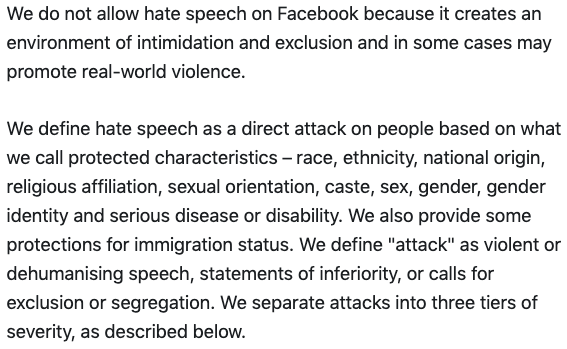
\includegraphics[width=\linewidth]{Chapter2/Figs/Facebook.png}
    \caption*{(a) Facebook}
  \end{minipage}\hfill
  \begin{minipage}{0.32\textwidth}
    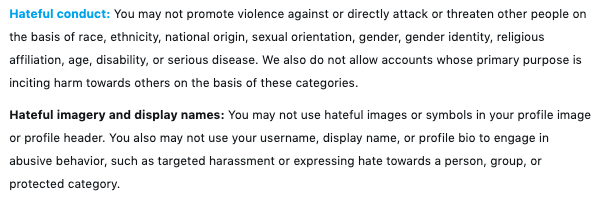
\includegraphics[width=\linewidth]{Chapter2/Figs/Twitter.png}
    \caption*{(b) Twitter}
  \end{minipage}\hfill
  \begin{minipage}{0.32\textwidth}
    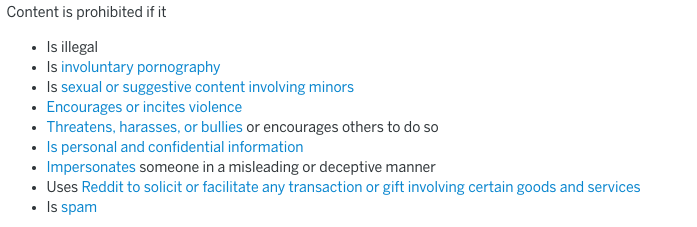
\includegraphics[width=\linewidth]{Chapter2/Figs/Reddit.png}
    \caption*{(c) Reddit}
  \end{minipage}\hfill
  \caption{Excerpts of policy on prohibited content and hate speech from Facebook, Twitter, and Reddit.}
  \label{fig:policies}
\end{figure}

In all three excerpts of the policies, we see a prohibition of content which attacks others, Reddit's policy on encouraging and inciting violence they further outline that users should not post content that\footnote{for the full policy see \url{https://www.reddithelp.com/en/categories/rules-reporting/account-and-community-restrictions/do-not-post-violent-content}}

\begin{aquote}
  [\dots] that encourages, glorifies, incites, or calls for violence or physical harm against an individual or a group of people
\end{aquote}

establishing similar outlines for acceptable conduct as seen on Twitter and Facebook. Facebook note in their Community Standards Enforcement Report\footnote{See report here: \url{https://transparency.facebook.com/community-standards-enforcement\#hate-speech}} that they acted on $4$ million items for hate speech and $2.8$ million items for bullying and harassment in the period of January to March 2019. The report does not detail the number of user reports received, nor the amount of content which was not removed.\footnote{Acted on here means acknowledging that the content does violate community standards yet and an action was taken by Facebook.} Considering the scale of the items which have actions taken for different kinds of abuse, there is an incentive to automate allow for some automation to guide the attentions of human moderators or decrease the number items which moderators need to consider.\footnote{The Community Standards Enforcement Report details that automated systems are deployed but do not detail the performances of the system in terms of accuracy, precision, or recall.}

While Facebook report high numbers of removals, the performance of their (human and automated) moderation practices have been the source of criticism as a number of activists have reported being temporarily banned for speaking about racial discrimination while abuse and discrimination received is not addressed \citep{Sharif:2019} and common users noting that simply talking about race may mean that your post is removed, particularly if the poster is not white \citep{Guynn:2019}. A report from Propublica details that the policies of Facebook in determining whether a post violates community guidelines, by seeking global standards, effectively ``protect the people who least need it and take it away from those who really need it.''\citep{Angwin:2017}

%In fact, automated processes are used for $14.1\%$ of actioned content for harassment and bullying and $64.4\%$ for hate speech. Considering then the number of appeals, for hate speech more than $1$ millioned actioned items were appealed, and $496$ thousand were appealed for bullying and harassment. Numbers are not provided for the precision of the automated systems.

\subsection{Regulation} \zw{Limit the length of this as this will be less prominent in the thesis}
In recent years several different governments have sought to address the issue of online abuse, for isntance the British Home Office \citep{HomeOffice:2016} and the European Commission \citep{EUCommission:2016} gave guidelines and a call to action to social media networks. In a different approach, the German government passed the Network Enforcement Act (NetzDG) \citep{NetzDG:2017} in an aim to provide regulation to curb online abuse and misinformation. The regulation states that online platforms will face fines if they systematically fail to remove hate speech within $24$ hours.\vspace{5mm}

Building on this, the European Union is currently considering regulation on disseminating terrorist content which may have implications on hate speech and how social media platforms deal with issues such as hate speech \citep{EUCommission:2018} through the difficulty in distinguishing between content which promotes terrorism and content which is simply hateful - a consideration which is highlighted in the response from the European Union Agency for Fundemental Rights (FRA). In their opinion, the FRA suggest that the proposed regulation should provide a clear definition of terrorist content which limits it to inciting or promoting terrorist activities or providing instructions on the making or use of weapons \citep{FRA:2019}. A key point of the regulation states that the platforms must remove content within $1$ hour of receiving notice from a trusted authority.\vspace{5mm}

More severely, two bills on sex trafficking were passed in the United States of America, namely the Stop Enabling Sex Traffickers Act (SESTA) and the Fight Online Sex Trafficking Act (FOSTA). These two bills aim to prevent sex trafficking by removing sexual solicitation online. While the critiques of the bills are numerous for flaws in their conceptualisations \citep{Romano:2018}, impact on criminal investigative work \citep{Q:2018} and the consequences for sex workers - including missing persons and deaths of sex workers \citep{Blue:2018,Simon:2018}, the implications of the bills are far greater in three espects:

\begin{enumerate}
  \item{The bills weaken \citep{Romano:2018,Stryker:2018} in Section 230 of the Communications Decency Act (CDA) - which holds that computer service providers are not publishers and thus not liable for content on the platform \citep{EFF:230},}
  \item{the bills are effective retroactively \citep{Stryker:2018}, therefore necessitating moderation of both new and historic content, and}
  \item{the bills do not require a request to remove content prior to potential consequences for not upholding the laws.}
\end{enumerate}

While the weakening of Section 230 of the CDA falls in line with the European and German regulations by holding social media companies accountable for the content on their platforms, the European and German initiatives require are designed such that social media platforms respond to flagging and requests for content removal. Furthermore they are not in effect retroactively. These differences strongly encourage the use of machine learning to be applied regardless of the precision of the systems.\vspace{5mm}

% \subsection{Court Cases}  \zw{Limit the length of this as this will be less prominent in the thesis}
%
% Considering pressures to turn to automation, it is relevant to consider the class action lawsuit against Facebook\footnote{see Scola v. Facebook, Inc and Pro Unliminted, Inc., 2018, Civil Action No.: CIV0513} and the lawsuit Microsoft\footnote{See Soto and Blauert v. Microsoft, 2017, Case No.: 16-2-31049-4} by former content moderators from each company. Both lawsuits will be going forward and have not been settled. In both lawsuits, the plaintiffs report that they suffer from Post-Traumatic Stress Disorder as a result of being exposed to content such as beheadings and child pornography coupled with insufficient support and debriefing opportunities.
%
% \subsection{Collective Pressures}
%
% In the previous subsections we outline different three different pressures for content moderation on social media companies: Regulatory pressure, legal pressures, and pressures of volume. These pressures collectively generate a strong motive for deploying automated systems for content moderation including identifying abuse and hate speech. Considering however the issue of abuse, often context is required. However, while there may be an strong desire for automated systems, the issues in the impact on marginalized people highlight that uniform rules to apply to all groups may in fact effectively be discriminatory, which calls for systems to be developed thoughtfully with the knowledge that they may be discriminatory.
%
% TODO Look at this again later. It doesn't fit here. \cite{banks:2010} suggest that the lack of accountability, the immediacy, and global nature of the internet has allowed for it to become ``an ideal tool for extremists and hate mongers to promote hate''. In addition, it was the hopes of Facebook that increased accountability would lead to a decrease in hate speech \citep{Levine:2013}.


\section{Summary}
In this chapter, we have introduced several key notions and concepts that will lay a theoretical and philosophical foundation of our work. Specifically, we introduce the concepts of oppression, privilege, and intersectionality. These concepts will be implicitly built into our work, in the cases where it is not made explicit. In addition, we introduce considerations on anonymity and pseudonymity which will be utilised in some projects undertaken in this PhD and how they will be used. Finally, we have introduced the legal and social contexts of content moderation and introduce issues that may arise from implementing systems without concern to being potentially discriminatory.

% !TEX root = ../thesis.tex
\chapter{Computational Background}\label{chap:nlp}

\ifpdf
    \graphicspath{{Chapter3/Figs/Raster/}{Chapter3/Figs/PDF/}{Chapter3/Figs/}}
\else
    \graphicspath{{Chapter3/Figs/Vector/}{Chapter3/Figs/}}
\fi

In this chapter I introduce related work in Natural Language Processing (NLP) and theoretical background on the machine learning methods that I use throughout this dissertation.

% \subsection{Abusive Language Detection}
% % \zw{Update this}
% % Abusive language detection is a growing field of inquiry. Much off the early work focused on cyber-bullying \citep{Chen:2012,Cho:2013,Reynolds:2011} and profanity \citep{Sood:profanity:2012,Sood:2013} with little focus on demographically specified abuse, such as racism, sexism, and anti-Semitism \citep{Warner:2012}. More recently, work on demographically specified has surfaced as an independent task \citep{Waseem:2016,Waseem-Hovy:2016,Davidson:2017,Tulkens:2015,Agarwal:2016,Silva:2016,Park:2017,Samghabadi:2017}.
%
% A large part of the previous work on hate speech detection has primarily touched upon surface level analysis of abusive language, leaving much room for work to be done. A large effort has been expended in attempting to define annotation schemes. \cite{Waseem-Hovy:2016} proposed guidelines derived from gender studies \citep{McIntosh:1988} where a document is labeled as hate speech, if it fails any point in the guidelines.
%
% \cite{Waseem-Hovy:2016} released a data set for sexist and racist speech on social media which is annotated using their guidelines. In their paper, they investigate the impact of several features on detecting racism and sexism. They find that characters are more discriminative for hate speech detection in line with the findings of \cite{Mehdad:2016}. In addition, \cite{Waseem-Hovy:2016} find that information about a users gender can slightly improve classification performance, however they also find that adding location information slightly harms a classifiers performance. In addition, they find that information on length negatively impacts a classifiers performance.
%
% \cite{Ross:2016} investigate annotator agreement for anti-refugee sentiment. They instruct their annotators to follow the Twitter's guidelines for hateful content. They find that on a data set of 541 tweets, they achieve a very poor inter-annotator agreement, suggesting that it is necessary for clear and concise guidelines for annotation of abusive language.
%
% Building on the work of \cite{Waseem-Hovy:2016} and \cite{Ross:2016}, \cite{Waseem:2016} consider the impact of annotators' knowledge of hate speech for building models for hate speech detection; they find that employing feminist annotators for labeling data sets allows for more consistent annotations and models as compared to annotators that are not screened for political opinion. \cite{Waseem:2016} consider the application of features from sarcasm detection, using Author Historical Salient Terms (AHST) proposed by \cite{Bamman:2015}. The feature is generated by computing TF-IDF scores for each user and selecting the 100 highest weighted terms. If a term then occurs both in the document being analyzed and in the AHST. \cite{Waseem:2016} find that AHST performs extremely poorly, suggesting that hate speech may generally be a one off event, rather than a continuous stream of abuse. It is our contention that another reason AHST might not work is due to the data set employed being highly imbalanced.
%
% \cite{Davidson:2017} seek to break down the task of hate speech detection into offensive language and hate speech and obtain labels for a Twitter data set using crowd sourced labor on CrowdFlower.
%
% More recently \cite{Badjatiya:2017} trained a deep convolutional neural network (CNN) on the data set annotated by \cite{Waseem-Hovy:2016}. By using a CNN on the data set \cite{Badjatiya:2017} obtain a significant improvement on Waseem and Hovy's (2016) scores improving the F1 score from  $73.89$ to $93.00$. Given the large increase in scores it is prudent to consider any potential errors. The data set \cite{Badjatiya:2017} employ, is highly imbalanced with the positive classes occupying a small minority of the labeled data, there is a risk that their model performs extremely well on the negative class but does not perform well on the positive classes. However, no error analysis is provided in the paper.
%
% In continuation of the results obtained by \cite{Badjatiya:2017}, \cite{Park:2017} compare using a two-step logistic regression classification, and a single step CNN approach to detecting hate speech. In the single step CNN, the specific form of hate speech is directly predicted, while in the two-step classification scenario, first a classifier is trained to identify whether a document contains abuse followed by predicting the specific type of abuse it is.
%
% A different approach is attempted by \cite{Waseem:2018}, in which they seek to combine three different datasets for abusive language detection using multi-task learning. With a hypothesis that abuse will differ between geographic and cultural locales, they seek to employ disjoint datasets and train two models, one for each data set that share parameters. We will seek to extend this work to employ more data sets of abusive language as well as related tasks, such as sentiment analysis.
%
% Finally, \cite{Jha:2017} break ``sexism'' down into benevolent and hostile sexism. They apply the ambivalent sexism theory as proposed by \cite{Glick:1996}. The ambivalent sexism theory suggests that there are two forms of sexism, benevolent sexism, which on a surface level speaks positively on women, but on a deeper level seeks to assert their inferiority, and hostile sexism, which expresses a strictly negative point of view on women. The following examples illustrate benevolent and hostile sexism respectively: ``Women are like flowers who need to be cherished.'' and ``Jus gonna say it..again..DUMB BITCH! \#MKR''.\vspace{5mm}
%
% As online platforms seek to remove abuse occurring on their platform, data sets that have been gathered and annotated may have the abusive documents removed, thus requiring several rounds of re-annotation of abusive language. In an attempt to deal with this, we will experiment with using documents that are assumed have a higher chance of being abusive as they are posted in forums that are known to abusive. Using these documents we will seek to build different forms of embeddings and evaluating on previously annotated data. Further, in an attempt to mitigate annotator needs, we will build an abusive language potential system which utilizes supervised methods for Named Entity Recognition (NER), Gender Identification \citep{Sap:2014}, and sentiment analysis amongst other methods. The goal of this is to identify the probability that a document has potential to contain abusive content, in efforts to exact greater control over what documents an annotator is faced with. Additionally, such a system will allow us to identify documents which are clearly abusive. Thus, we will be able to provide an automated method to create a seed set of positive documents for abusive language detection.
\section{Abusive Language Detection}

% Introduce the field of abusive language detection
In recent years, the computational study of online abuse has seen a rapid increase in the number of papers dedicated starting with a handful of papers prior to $2016$ to a thriving research field with numerous papers, shared tasks, and workshops \citep{Vidgen:2020}. In spite of the growth in research dedicated to the detection of online abuse, the research field is still in its infancy with a number of open questions, including questions around definition of the task, annotation guidelines, and modelling techniques.
The earliest work in the field sought to address questions of cyber-bullying \citep{Chen:2012,Cho:2013,Reynolds:2011} and profanity \citep{Sood:profanity:2012,Sood:2013} with sparing focus on demographically specified abuse, such as racism, sexism, and anti-Semitism \citep{Warner:2012}. More recently, work on demographically specified abuse has surfaced as an independent task \citep{Tulkens:2015,Waseem:2016,Waseem-Hovy:2016,Park:2017,Samghabadi:2017,Karan:2018,Gorrell:2018,Stoop:2019,Meyer:2019,Palmer:2020,Vidgen:2020}. As a consequence of increased visibility of hate speech and abuse on online platforms, the academic inquiry into the computational detection has grown along with the regulatory responses \citep{Regulatory stuff: NetzDG, EUcommision on hate speech}.

Early, and contemporary computational work, has seen a great deal of focus to central questions around the task: how do we annotate and create datasets \citep{Waseem-Hovy:2016,Waseem:2017,Vidgen:2020} and understanding annotator interaction and performance \citep{Ross:2016,Waseem:2016,Vidgen:dynabench:2021}.
Early work focused on questions of marginalisation and oppression, for instance through the work of \citet{Waseem-Hovy:2016} who base their annotation on works in gender studies and critical race theory, and collect data based on gendered and racialised abuse; more recently data collection and annotation processes have moved towards a demographically blind process. Such early work was inspired by the marginalisation of certain bodies and the desire to develop computational tools to protect marginalised people \citep{Warner:2012}.marginalisation of certain bodies and the desire to develop computational tools to protect marginalised people \citep{Warner:2012}.
More recent work has instead directed its focus to demographically blind approaches to data collection and annotation, succumbing to ``marginalisation-blind'' annotation processes and guidelines. Although processes that do not take marginalisation into account, but instead seek to treat every group equally provide an allure of fairness, they also encode dominant discourse on abuse with the subsequent result of the resistance to oppression and marginalisation being treated the same as marginalisation. In concert with the growing evidence of racially biased content moderation tools \citep{Waseem:2018,Davidson:2019}, demographically blind annotation criteria and data curation pose a threat to the goal of developing tools that aid in ensuring people from the right from persecution. One such example is presented by \citet{Salminen:2018} who develop a taxonomy that includes ``anti-white'' as a target of hate on par with anti-Black hate in spite of whiteness as a hegemonic entity that marginalises \citep{McIntosh:1988}.
A result of this are egregious annotation choice, such as ``The  white  will  always  steal;  FUCK  YOU  TO  ALL  WHITES  RACIST'' labelled as hate speech \citep{Salminen:2018}, in spite of the comment speaking to ongoing racism and the historical exploitation enacted by white societies (e.g. the theft of cultural artefacts from colonised territories \citep{Frost:2019}, the numerous genocides committed by imperialistic colonial states \citep{Weisbord:2003}, and the theft of bodies in the transatlantic slave trade). Moreover, and perhaps of even greater concern, the annotation and curation processes of \citet{Salminen:2018} result in data responding to the abuse of authority committed by police as hate, in one such example they identify the following comment as hate ``did to that poor guy. 10 s of pepper spray directly into the face, run over foot etc. equal it up a little bit, except for the detail of having a fucking stroke. So it still wouldn’t be exactly what the guy went through. Fucking discusting. They get a hard on power tripping others. They are just fucking cowards'', in all likelihood due to the aggressive nature of the comment.

Through such demographically uninformed processes of curating and making data, a danger of erasure of past and ongoing marginalisation and responses to it as well as critical responses to the violent abuse of authority as ``hate speech'' that should be subject to content moderation. The question of automated hate speech detection thus, for works such as \citet{Salminen:2018} is no longer ensuring the right to not be persecuted but instead insuring that processes of marginalisation remain unchallenged.
For these reasons, I use the datasets released in early work, specifically I use the \textit{Offence} dataset \citep{Davidson:2017}, \textit{Toxicity} dataset \citep{Wulczyn:2017}, and \textit{Hate Speech} dataset \citep{Waseem-Hovy:2016} in all computational chapters. For \autoref{chap:liwc} which examines the influence and generalisability of vocabulary manipulation, I also use the \textit{Hate Expert} \citep{Waseem:2016} and the \textit{StormFront} \citep{Garcia:2019} datasets. Each of these datasets share the common attributes that they are collected either from spaces that are hateful towards marginalised groups or have considerations of marginalisation encoded into the annotation guidelines. In \autoref{chap:mtl} I also use three datasets that are labelled for abuse but instead to tasks that are seemingly related. First, I use the \textit{Argument Base} dataset \citep{Oraby_fact_feel:2017}, the second dataset (\textit{Sarcasm}) is developed for sarcasm detection \citep{Oraby_sarcasm:2017}, and the final dataset, \textit{Moral}, examines the moral sentiments
In an early effort to address issues of annotator biases and under-sampling of some forms of data in the data curation process, \citet{Waseem:2017} propose a typology of abuse that aims to categorise abuse by how it is characterised rather than determining the exact form of abuse.
To this end, \citet{Waseem:2017} present a 2-dimensional typology of hate; the first dimension operates along implicit and explicitly expressed hate. Implicitly communicated hate, \citet{Waseem:2017} argue is hate that is communicated through subversive means by using code words and communicating implicit biases. Explicit abuse on the other hand is explicit in its intention to abuse, e.g. through the use of slurs. The second dimension concerns itself with the target of abuse that can either be a generalized other, or a specific group, the former category detailing abuse that is targeted towards small groups and individuals while the latter is aimed at generalised targets, e.g. larger demographics.
It's important to note that content may be simultaneously explicit and implicit, directed and generalised \citep{Waseem:2017}. For instance, content that implicitly targets Muslims, may simultaneously explicitly target a specific group of women.

\begin{table*}[ht]
\centering
\begin{tabular}{p{\textwidth/30}|p{0.45\textwidth}|p{0.45\textwidth}}
  & \textit{Explicit}    & \textit{Implicit} \\\hline
    \multirow{4}{*}{\rotatebox[origin=c]{90}{\textit{Directed}}}    &   {\scriptsize``Go kill yourself'',  ``You're a sad little f*ck'' \citep{Hee:2015a}}, \newline {\scriptsize ``@User shut yo beaner ass up sp*c and hop your f*ggot ass back across the border little n*gga''  \citep{Davidson:2017}}, \newline {\scriptsize ``Youre one of the ugliest b*tches Ive ever fucking seen'' \citep{Kontostathis:2013}}. & {\scriptsize ``Hey Brendan, you look gorgeous today. What beauty salon did you visit?'' \citep{dinakar2012common}, \newline ``(((@User))) and what is your job?  Writing cuck articles and slurping Google balls?  \#Dumbgoogles'' \citep{Hine:2016},\newline  ``you're intelligence is so breathtaking!!!!!!'' \citep{dinakar2011modeling}}\\\hline
  \multirow{5}{*}{\rotatebox[origin=c]{90}{\textit{Generalized}}} & {\scriptsize``I am surprised they reported on this crap who cares about another dead n*gger?'', ``300 missiles are cool! Love to see um launched into Tel Aviv! Kill all the g*ys there!'' \citep{Nobata:2016}, \newline ``So an 11 year old n*gger girl killed herself over my tweets? \^ \_ \^\ thats another n*gger off the streets!!'' \citep{Kwok:2013}}. & {\scriptsize``Totally fed up with the way this country has turned into a haven for terrorists. Send them all back home.'' \citep{burnap2015cyber}, \newline ``Gas the skypes'' \citep{magu2017detecting}, \newline ``most of them come north and are good at just mowing lawns'' \citep{dinakar2011modeling}} \\
\end{tabular}
  \caption{Typology of abusive language presented by \citep{Waseem:2017}.}
\label{tab:typology}
\end{table*}

Modelling for automated hate speech detection has also undergone a development from early to contemporary work. Early work was primarily focused on feature-based modelling \citep[e.g.][]{Waseem-Hovy:2016,Waseem:2016,Davidson:2017,Sahlgren:2018} whereas subsequent work has directed a greater attention to neural network based approaches \citep[e.g.][]{Kolhatkar:2021,Waseem:2018,Gamback:2017,Badjatiya:2017}. In this dissertation I follow a similar pattern of developing baseline models from feature-based models and suggest neural network architectures as extensions and improvements on these. In early work, Logistic Regression (LR) and Support Vector Machines (SVM) were the most frequently used models. As the scholarship has developed, specific types of neural networks have come to dominate the modelling, namely Convolutional Neural Networks and Long-Short Term Memory networks. In each chapter, I perform the review of the models that are pertinent to the work in the chapter. Here instead I provide a theoretical overview of the models, their components (e.g. dropout and activation functions) and their intended functionalities (i.e. the kind of data that they are designed to operate on and which assumptions are built into the model architectures).

\subsection{Datasets}\label{sec:datasets}

Here I provide an overview of the different datasets that are used throughout this dissertation. For each dataset, I introduce the curation rationale, the source of the datasets, the annotation guidelines, annotator selection, and finally how each of these dimensions influence the resulting dataset. In \autoref{sec:abuse_data} I describe the datasets annotated for hate speech and abuse and then in \autoref{sec:mtl_data}, I turn to the datasets used for the auxiliary tasks for \autoref{chap:mtl}.

\subsubsection{Hate speech and abuse datasets}\label{sub:abuse_data}

\paragraph*{Hate Speech} Published as the first publicly available dataset for hate speech and abusive language detection, \citet{Waseem-Hovy:2016} developed a dataset for detecting abuse towards gendered and racialised minorities. In an interview in the Let's Chat Ethics Podcast, Zeerak Waseem shared that the initial motivation for developing the dataset was the somewhat na{\"i}ve hope to address online harassment as experienced by women during \#GamerGate, a harassment campaign against female game developers and games journalists \citep{Massanari:2015}. This aim of developing tools that can protect marginalised people is apparent in the data sampling and the source of data. As a large amount of the GamerGate abuse occurred on Twitter, \citet{Waseem-Hovy:2016} use Twitter as a source of their data, collecting $16,914$ tweets labelled as ``sexist'', ``racist'', and ``neither''.
In efforts to ensure that their collected and annotated sample contains gendered and racialised abuse, they bootstrap their corpus collection by first search for common slurs against women, ethnic minorities, religious minorities, and sexual minorities to identify the salient terms and users for scraping.
To annotate this dataset, with the target group in mind, \citet{Waseem-Hovy:2016} develop $11$ questions to test whether a comment is hateful or not.
This set of questions focuses on breadth in the types of hate expressed rather than depth in each type. This is apparent as the tests ranges from asking about explicit forms of hate, such as the use of slurs to implicit forms like questions around stereotyping and the use of straw man arguments in criticisms of minorities.
\citet{Waseem-Hovy:2016} annotate their dataset and have their annotations verified by an external annotator.
Collectively, these decisions are made to ensure that there was a diversity in the forms of hate in addition to the sources. However, as they note, the racist abuse only comes from $9$ different accounts. Moreover, as salient terms were sampled for annotation, some terms (i.e. the hashtag for the Australian TV show My Kitchen Rules) are over-represented in the data. In spite of these issues, the annotations in this dataset are \textit{embodied} within the context of critical race and gender studies perspectives on abuse.

\paragraph*{Hate Expert} In an extension of the dataset proposed by \citet{Waseem-Hovy:2016}, \citet{Waseem:2016} sample $6,909$ tweets from the original scrape and have it annotated by two groups, in efforts to understand the influence of annotator biases. The first group consisted of ``feminist and anti-racism activists'' \citep{Waseem:2016} who annotate the sample of the dataset with one of four labels ``racist'', ``sexist'', ``both'', and ``neither''. The second group of annotators were recruited from CrowdFlower to re-annotate the sample annotated by the first group.\footnote{CrowdFlower has since been renamed Appen.}
The label set was expanded by \citet{Waseem:2016} to include the category ``both'', in acknowledgement that marginalisation can be expressed across multiple dimensions, in an \textit{Intersectional} manner. Comparing models trained on each group of annotators, \citet{Waseem:2016} find that models that use the annotations of the first group consistently outperform models trained on the second. \citet{Waseem:2016} argue that the reason for this difference is that models trained on the former group benefit from similarities in the understanding of hate speech, whereas the distinct subjective positionalities of the latter group, that does not have a salient unifying characteristic beyond their work on a crowd-sourcing platform, produces internally inconsistencies in labelling that render it harder for models to consistently identify patterns that they can learn from.
In presenting this dataset, \citet{Waseem:2016} propose that ideologues can take similar positions on a topic, given their subjective positionalities. They argue that only through a principled understanding of hate speech is it possible to annotate reliably for hate speech and that crowd-sourced annotations for hate speech display inconsistencies that to some degree erases the meaning of the term.
In using this dataset for this dissertation, I use the annotations provided by the feminist and anti-racist activists.

\paragraph*{Offence} Departing from the question of forms of hate speech and gender studies and critical race theory based annotation guidelines, \citet{Davidson:2017} turn instead to ask where the distinction between simply ``offensive'' speech and ``hate speech''.
Using a list of terms from Hatebase\footnote{Hatebase.org is a website that crowd-sources slurs and insulting turns of phrase. Due to marginalised people being disproportionately targeted, there is a distributional skew towards terms that target marginalised people in the number of terms.} to identify $33,458$ users whose tweets they sample.
From these users, they randomly sample $25,000$ tweets for annotation by CrowdFlower workers, resulting in $24,802$ annotated tweets. The crowd-workers were given guidelines to aid them in distinguishing between ``offensive content'', ``hateful content'' or ``neither offensive or hateful'', selecting only one for each tweet. \citet{Davidson:2017} instruct their annotators that hate speech is speech that ``is used in reference to certain groups that expresses hatred towards the group or is intended to be derogatory, to humiliate, or to insult the members of the group''. Moreover, they provide examples of such content which includes the straightforward ``Need to send these w******s back to their country''\footnote{Censoring of the slur is mine.} and the more conflicted ``I hate white trash''. The conflict in the latter stems from it being unclear whether the emphasis is on class-based hate or if it is targeting white people. While the former is less contentious, the latter would imply that white people too are targets of marginalisation on the basis of their race. However, as numerous scholars have argued, whiteness is the hegemonic force that marginalises \citep{CRT scholars}.
``Offensive'' content is provided as an alternative, less serious form of potentially unwanted content. This group is defined in contrast to the hateful class ``[o]ffensive content might use some of the same words we associate with hate speech but do not \textit{necessarily} constitute hate speech because the words are not used in the same context as ``hate speech````.\footnote{Emphasis added.}
From this definition it's clear that in spite of the instruction to select only one category, \citet{Davidson:2017} acknowledge that there is a potential overlap between offensive language and hate speech. 
Moreover, unlike the annotation guidelines proposed by \citet{Waseem-Hovy:2016}, the definition of offensive draws in the question of context. Illustrating this point, \citet{Davidson:2017} provide the following example ``Oh shush you know I love you f****t''. This use of context, provides space for inoffensive uses of slurs and insulting terms e.g. for reclaimed and in-group uses, a space that the annotation guidelines of \citet{Waseem-Hovy:2016} does not afford.
With the annotators being selected from CrowdFlower, the issues of multiple distinct ideologues in the annotator pool raised by \citet{Waseem:2016} are likely also manifest in this dataset.
However, as the dataset offers a space within which one can utter offensive but not hateful messages, it also offers the space to live spaces that dominant discourse on acceptability of language use would deem as unacceptable.\footnote{By dominant discourses on acceptability, I refer to what mainstream discourses deem as acceptable and unacceptable manners of speaking. However, such a discourses are internally inconsistent, as \citet{Oliva:2020} show, acceptable speech can come to include neo-nazi and white supremacist speech that threaten social cohesion while deeming speech by queer communities as toxic and inherently holding greater threat to the boundaries within which society should operate.}
In consideration of the marginalisation of queer people and people of colour, this dataset thus offers space for their uninterrupted existence. However, as the dataset is labelled for a multi-class classification problem, where a single label is assigned to each document, the dataset does not afford space to be exposed to hate speech in such contested spaces.

\paragraph*{Toxicity} Starting from a similar point as \citet{Davidson:2017}, \citet{Wulczyn:2017} develop a dataset  of $115,737$ comments to understand which types of conversations are likely to make users depart from the conversation. Departing from the early tradition of using Twitter as a source of data, \citet{Wulczyn:2017} consider the Wikipedia editor discussion pages. Taking a narrow view of behaviours that inhibits participation in conversations, \citet{Wulczyn:2017} focus on personal attacks and harassment, specifically asking their annotators whether which entity (the participant or a third party) is the subject of the attack. As a last positive category, they include whether it is ``[a]nother kind of attack or harassment'', thus relegating all forms of harassment that are not directed at specific individuals to a residual category. The dataset thus is comprised of ``personal attacks'' and ``other forms of harassment''. As the study is specifically grounded in identifying personal attacks, this categorisation of various forms of personal attacks and a residual category as positive instances is in line with the aims of the data, if not the description.
Using this definition, \citet{Wulczyn:2017} select a random sample of $37,611$ and have it refereed by $10$ annotators for personal attacks, resulting in only $0.9\%$ of the labelled data being assigned the positive label. Subsequently, they identify $78,126$ comments that had been made by users whose comments were moderated from the discussion pages, for each user taking $5$ comments that they made around the moderated comment, and similarly subject them to annotation this time resulting in the positive class occupying $16.9\%$ of the labelled data.
Similarly to \citet{Waseem:2016} and \citet{Davidson:2017}, \citet{Wulczyn:2017} use CrowdFlower to obtain their annotations and subsequently are prone to similar issues in their data. However, to curb such issues they obtain $10$ annotations for each comment, allowing to compute a majority vote that takes a broader perspective on the comment into account. In spite of this approach, where those annotators are from and what their position on personal attacks are, and their ability to identify subtle attacks, still remain uncertain resulting in a dataset that may take a global position or a culturally grounded position on identifying personal attacks, e.g. if a large subset of annotators live in India, a subset of the data may very well reflect Indian perceptions of personal attacks.
The resulting dataset has been constructed to understand which comments are likely to turn discussions ``toxic'' as a result of personal attacks. Through the use of $10$ annotators for each comment, \citet{Wulczyn:2017} aim for a global understanding of toxicity derived, in part, from personal attacks.
Similarly to \citet{Davidson:2017}, there appear to be no consideration of the experiences of abuse against marginalised communities.
Considering Wikipedia's well documented issues with being a hostile space to women \citep{Torres:2016} and the distribution of gender crowd-workers often veering towards a greater representation of men than women \citep{Posch:2018}, the lack of such a consideration may further entrench subjective positions that are hostile towards women into the datasets and subsequently into the models.

\paragraph*{StormFront} Focusing on the white supremacist web-forum StormFront, \citet{Garcia:2019} collect a dataset of $10,568$ sentences annotated by three of the authors for containing hateful utterances. Similarly to \citet{Davidson:2017} and \citet{Wulczyn:2016}, \citet{Garcia:2019} employ a marginalisation-blind definition and understanding of hate speech. In the case of a white supremacist web-forum, employing a marginalisation-blind definition is unlikely to be challenged as the participants are unlikely to engage in derogation against white, straight, cisgender men.
The decision for using StormFront as a source of data was motivated by the prevalence of ``pseudo-rational discussions of race''.
Moreover, this dataset further distinguishes itself from prior datasets by annotating on a sentence level.
The authors argue that annotating on a sentence level can reduce the confounding factors by only addressing content which is explicitly hateful.
While this may, in some instances have little effect as the surrounding sentences bear no impact on whether a sentence is hateful. This particularly holds for explicit hate speech.
However, for subtle forms of hate speech, conducting sentence level annotation may obscure hate that is only apparent when considering a post in its entirety rather than its sentence level components. In order to address this issue, \citet{Garcia:2019} introduce a ``related'' tag which is to be used when individual sentences do not convey hate but the combination of several sentences in sequence do convey hate.
This method for mitigation does not account for longer sequences of sentences that convey hate, as is often the case for subtle forms of hate speech and dog whistles.
Moreover, as \citet{Garcia:2019} take a very conservative position on what constitutes hate, for instance, the use of a derogatory term, on a white supremacist web-forum, ``cannot be said to be a deliberate attack, taken without any more context, despite it likely being offensive.'' For this reason, \citet{Garcia:2019} argue that simply the occurrence of slurs weaponised against marginalised communities cannot be said to be hateful.
Thus, while initially side-stepping the issue of marginalisation-blind definitions by sourcing data from a white supremacist web-forum, it is softly reintroduced by taking a conservative stance on what constitutes hate.

\subsubsection{Non-abuse datasets}\label{sec:mtl_data}

\paragraph*{Sarcasm} \citet{Oraby_sarcasm:2016} develop a dataset for sarcasm detection in dialogues. The dataset was developed in order to address the lack annotation for subtypes of sarcasm, i.e. rhetorical questions and hyperbole, at scale in previous datasets.
Sourcing their data from the Internet Argument Corpus (IAC) \citep{Abbott:2016}, \citet{Oraby_sarcasm:2016} annotate their data for ``generic sarcasm, rhetorical questions, and hyperbole''.
In order to generate a dataset from the IAC, \citet{Oraby_sarcasm:2016} train a ``weakly-supervised pattern learner'' \citep{Oraby_sarcasm:2016} to identify a set of $30,000$ posts, filtering two thirds of the posts that don't contain any ``not-sarcastic'' cues and annotate the remaining $11,040$ posts in quote-response pairs for annotation on Amazon Mechanical Turk.
Similarly to the abusive language datasets annotated on CrowdFlower, this choice of annotators can introduce biases stemming from the subjective embodiments of the human annotators and the geo-cultural contexts in which they exist.
Following the annotation process a dataset of $6,520$ posts (with a $50\%$ split of sarcastic and not-sarcastic posts) is obtaned and released.
Examining the dataset for suitability for machine learning experiments, \citet{Oraby_sarcasm:2016} train a linear SVM with Stochastic Gradient Descent (SGD) training and L2 regularisation obtaining F1-score of $0.74$ using features derived from Word2Vec \citep{Mikolov:2013}.

\paragraph*{Argument Basis} Investigating the characteristics of factual and emotional argumentation styles, \citet{Oraby_fact_feel:2015} also draw on the IAC as the source of data. Considering quote-response pairs, each response is annotated for whether the argument presented in the response based primarily in fact or feeling.
\citet{Oraby_fact_feel:2015} present $10,003$ from the IAC for annotation by $5-7$ crowd-workers on Amazon Mechanical Turk for annotation selecting a value ranging from $-5$ to $5$ to indicate whether the response is a feeling or fact-based argument, where negative values indicate that the argument basis is dominated by an emotional argumentation style and positive values indicate a fact-based argument.
Each document is then given a binary label indicating its argument basis, where all texts with a score greater than $1$ are assigned as fact-based, all texts with a score lower than $-1$ are assigned to the feeling-based class, and all scores $[-1, 1]$ are discarded.
This annotation process results in $3,466$ fact-based and $2,382$ feeling-based documents.
Similarly to the previously examined datasets that utilise crowd-workers, this dataset is also subject to the contexts which the individual annotators exist within. For instance if an annotator is from a culture where feeling-based argumentation is not experienced as impassioned but instead supportive of facts, they may be likely to rate some documents as more fact-based than annotators who hail from cultures that emphasise fact-based argumentation would deem as relying on an emotional argumentation style.
The subjectivity of the annotation task may provide an explanation for why $4,155$ or more than $41\%$ of the documents are discarded due to being rated, in aggregate, as dominated by neither fact or emotion.

\paragraph*{Moral Sentiment} The final dataset used in this dissertation is the Moral Foundations Twitter Corpus \citep{Hoover:2019}. This dataset provides $35,108$ tweets annotated for $10$ different categories of moral sentiment, introducing the task of moral sentiment prediction.
A task, and dataset designed to allow psychology researchers to investigate the relationship between comments made around events and the moral foundations found in such comments made on Twitter.
% This task was introduced to explore the utility of NLP modelling techniques for psychology research, namely measuring psychologically relevant psychological constructs in tweets.
\citet{Hoover:2019} draw from research in psychology around human morality using a five-factor taxonomy that reveals insights into the moral foundations \citep{Graham:2009,Graham:2013} that underlie comments about and attitudes towards topics.
Each of the five factors are represented through a binary, where one end of the binary represents a virtue and is contrarian to the other, representing a vice.
\citet{Hoover:2019} argue that the human expression of vice and virtue are distinguishable from one another through distinct language use for each.
The five factors introduced are \texttt{care}, ``concerns related to caring for others'' and \texttt{harm}, ``concerns related to not harming others''; fairness, ``concerns related to fairness and equality'' and \texttt{cheating}, ``concerns related not not cheating or exploiting others''; \texttt{loyalty}, ``concerns related to prioritising one's ingroup'' and \texttt{betrayal}, ``concerns related to not betraying or abandoning one's ingroup''; \texttt{authority}, ``concerns related to submitting to authority and tradition'' and \texttt{subversion}, ``concerns related to not subverting authority or tradition''; \texttt{purity}, ``concerns related to maintaining the purity of sacred entities, such as the body or a relic'' and \texttt{degradation}, ``concerns focused on the contamination of such [sacred] entities.''
Noting that there is low occurrence of moral sentiments expressed in a random sample of tweets, \citet{Hoover:2019} collect tweets related seven different discourse domains where the occurrence of moral sentiment is likely to at a high rate: Black Lives Matter, All Lives Matter, Baltimore protests following the death of Freddie Gray, the 2016 presidential elections in the United States of America, hurricane Sandy, the \#MeToo movement, and offensive language, re-annotating a sample of \citet{Davidson:2017} for the moral sentiments.
For annotation, \citet{Hoover:2019} train $8$ undergraduate research assistants to an expert-level familiarity with the moral foundations taxonomy, annotating $4,000 - 6,000$ for each discourse domain. The annotators are trained through a training sessions and, in early stages, discussion surrounding annotator disagreement.  
The annotator selection procedure here thus develops on the suggestion of \citet{Waseem:2016} to use expert annotators to describing a means of training expert annotators for a highly subjective task. Interestingly, as the annotation process continues past early stages, annotator disagreements are not resolved, instead the authors opt for expressing the inherent subjectivity of the human annotation task.

\subsubsection{Non-English datasets for abuse}
\zw{See hatespeechdatasets.com and ACL anthology}

In this dissertation, I focus my attention to detecting abuse in English language datasets as my methods do not map to other languages. However, an important growing body of research and resources are being developed for other languages such as Arabic \citep{Arabic abuse papers}, Chinese \citep{Chinese abuse papers}, Croatian \citep{Croatian papers}, Danish \citep{Danish abuse data}, French \citep{French papers}, German \citep{German papers}, Greek \citep{Greek papers}, Indonesian \citep{Indonesian papers}, Italian \citep{Italian papers}, Polish \citep{Polish papers}, Portuguese \citep{Portuguese papers}, Slovene \citep{Slovenian papers}, Spanish \citep{Spanish papers}, Turkish \citep{Turkish papers}, and Urdu \citep{Urdu papers}. Beyond these mono-lingual resources and approaches, there is also a body of work dedicated to abuse in code-switching contexts \citep{Code switching papers}.

Developing models for each individual language, and in particular resources that address abuse that code-switches, require an attention to the particularities of the different languages and cultures, just as model development for English requires researchers to be attuned to the particularities and cultures represented in English language use.


\subsection{Generalisable Machine Learning Models for Abusive Language Detection}
A common criticism of many current computational methods for abuse detection is that they have poor generalisability onto other datasets. Although this issue of non-generalisability poses a serious issue for the abuse community, it has received relatively little attention \citep{Waseem:2016,Waseem:2018,Karan:2018,Wiegand:2019,Swamy:2019,Fortuna:2021,Glavas:2020} in comparison to single-dataset classifier performance. In each of the computational chapters (see \cref{chap:liwc,chap:mtl}), I also provide consideration of how well the trained models perform on out-of-domain datasets.
In the pursuit of models that generalise well onto other datasets, researchers have proposed a variety of architectures. As an initial investigation into the question of generalisability, \citet{Waseem:2016} note that the best performing classifier on the dataset they propose does not generalise well onto the \textit{Hate Speech} dataset, noting that the performance of their classifier drops by more than a $25\%$.
Using Multi-Task Learning (MTL),\footnote{Multi-task learning allows for training models using multiple different datasets, for distinct machine learning tasks, where one (main) task is given higher priority and all other tasks are treated as auxiliary tasks.} \citet{Waseem:2018} address the issue of poor generalisability between the \textit{Hate Speech} and \textit{Hate Expert} (combined into a single dataset) and the \textit{Offence} dataset, showing that a MTL framework can be used for training models that can generalise onto from one cultural context onto another. Moreover, considering the results posted by \citet{Waseem:2018}, it appears that there is a trade-off between well-performing in-domain models and well-performing cross-domain models, where cross-domain improvements appear to come at the cost of in-domain performance, where out-of-domain performance is computed by mapping the classes in the in-domain datasets to the out-of-domain dataset.

\citet{Karan:2018} further explore the question of cross-dataset generalisability using a linear SVM model. \citet{Karan:2018} approach the task of out-of-dataset performance as a classical domain adaptation task and use the FEDA framework \citep{Doume:2007}, finding that without significant procedures for domain adaptation, there is poor generalisability. Similarly to \citet{Waseem:2018}, \citet{Karan:2018} find that cross-domain performance comes at the cost of in-domain performances but with large out-of-domain improvements. One difference between \citet{Karan:2018} and the previously described studies is that \citet{Karan:2018} reduce the learning task to a binary classification task of ``abusive'' and ``non-abusive'' documents.

The last approach to generalisation I consider is the work by \citet{Fortuna:2021}. In this paper, the authors compare four different models for out-of-domain classification: a Bag-of-Words SVM model, a Continuous Bag-of-Words FastText model, a BERT model \citep{Devlin:2019}, and an ALBERT model \cite{Lan:2020}. The latter two being transformer-based language-models that are fined-tuned to the task of predicting abuse.
\citet{Fortuna:2021} propose a different class organisation to past studies, first they propose as generalised class organisation that collapse classes across datasets into a smaller, generalised subset that maps across datasets. For instance, the ``sexist'' class provided by \citet{Waseem-Hovy:2016} and the ``misogyny'' class provided by \citet{Fersini:2018} into a ``misogyny-sexism'' class. Each of the generalised classes are binarised to allow models trained with other standardised labels to predict on them.
Using these generalised classes, \citet{Fortuna:2021} show that by using methods that capture more complex word-interactions, out-of-domain performance generally improves within and out of domain, subject to the classification task.
Specifically, they find that when classes have significant overlaps across datasets in their rationalisation of what the are to represent then models trained on those classes will map well onto the rest.
Conversely, when the classes have a little overlap, the models will generalise poorly onto the new dataset.
Moreover, \citet{Fortuna:2021} identify that some dataset combinations produce poor generalisation between each other regardless of the models used.
This, in concert with their conclusion that dataset overlap and out-of-domain similarities are drivers of model generalisation has two implications.
First, current computational models can, to some degree, adapt onto new distributions and samples but models using words as input are poorly suited for learning general trends of a wide variety of abuse, including closely related concepts such as ``toxicity'' and ``severe toxicity'' \citep{Fortuna:2021}.
Second, as models do not generalise onto other concepts, even if closely related, research in the detection of online abuse must either develop methods that can generalise onto studying different objects and perspectives of online abuse, or datasets must be annotated following highly similar annotation guidelines at the cost of the depth and breadth of concepts that can be explored.

\section{Models}\label{sec:model_background}
% TODO Introduce modelling
% TODO Introduce Linear models: SVM, LR
% TODO Neural Networks: Single-task + MTL
% TODO LSTM (and recurrence)
% TODO MLP
% TODO CNN and pooling
% TODO Introduce vectorisation & tensorisation
% TODO Softmax, Losses (NLLL), Optimisers (SGD, ADAM, ADAMW, ASGD)
% TODO Hyper parameter tuning
% TODO Metrics: precision, recall, F1, accuracy
% TODO Fairness work
% TODO Limitations

In this section I provide an introduction to the different modelling techniques that I use throughout the dissertation.

\subsection{Data Encoding}

In order for models to read the data, it is necessary to provide the models with machine readable representations of the data. The first step to creating such machine readable representations is to provide each unique token with a numerical index.
The numerical index, and what it represents is a matter of how the data is pre-processed. For instance, in \cref{chap:liwc}, I represent tokens in three different ways.
First, I represent tokens using their surface form, that is each word is represented in its entirety following a tokenisation process where all words are lower-cased and punctuation markers are split from the word (see \cref{chap:liwc} for further pre-processing steps). Second, I take the surface forms of tokens computed and represent them as the categories of the Linguistic Inquiry and Word Count (LIWC) categories each token induces (see \cref{chap:liwc} for further detail). Finally, in \cref{chap:liwc,chap:mtl} I represent tokens as the subwords that they consist of. 
In this section, the sub-word forms while omitting the surface-token and LIWC-token forms as these rely on simple pre-processing and mapping steps that are described in more detail in \cref{chap:liwc}.

\subsubsection{Byte-Pair Embeddings}

Byte-Pair Encodings were introduced to the NLP comunity by \cite{Sennrich:2016} for the task of Neural Machine Translation to address the issue of out-of-vocabulary tokens. In this paper, the authors argue that for word-level machine translation there is not always a one-to-one relationship between a word in the source language and its translation into a target language. \citet{Sennrich:2016} illustrate this point through compound words, where a compound word represents a specific entity that is represented through multiple words in the source language, e.g. the German \textit{Abwasser\textbf{|}behandlungs\textbf{|}anlange} and its English translation \textit{sewage water treatment plant} \citep{Sennrich:2016}.
\citet{Sennrich:2016} propose to compute sub-words using the byte-pair encodings algorithm proposed by \citet{Gage:1994}. While the algorithm proposed by \citet{Gage:1994} operates on bytes and seeks to develop a new representation of bytes that can compress their representation, \citet{Sennrich:2016} seek to operate on the sub-units of words, that is a sequence of characters. In both cases, the algorithm operates by considering the input and identifying frequently occurring patterns that can be represented in terms of a single unit.
In efforts to obtain a sub-word representation, \citet{Sennrich:2016} initialise their algorithm initially with a vocabulary consisting of each unique character token in the dataset and then count all symbol pairs (e.g. character co-occurrences) and merge the most frequently occurring pairs and adding it to the vocabulary. This merging process is repeated a number of times, where the total number of merge operations is a hyper-parameter set by the designer of the sub-word representation. The size of the vocabulary following this process will be the size of the original vocabulary plus the number of merge operations that are set by the designers \citep{Sennrich:2016}
In terms of language, using sub-words to represent documents can minimise the number of out-of-vocabulary tokens in the validation and evaluation sets of a dataset, as the likelihood of a word not being represented decreases as it is broken down into its subwords.

In this dissertation, I use the pre-trained Byte-Pair Embeddings (BPE) developed by \citet{Heinzerling:2018}. These embeddings were trained for $275$ languages using the Wikipedia pages in each language as the source of data. \citet{Heinzerling:2018} provide embeddings for $1,000,\, 3,000,\, 5,000,\, 10,000,\, 25,000,\, 50,000,\, 100,000$, and $200,000$ merge operations with dimensions $25,\, 50,\, 100,\, 200$, and $300$. For all chapters in this dissertation, I choose the $300$ dimensional embeddings that have been subject to $200,000$ merge operations

\subsection{Strategies against over-fitting}\label{sec:anti-overfit}

Machine learning models are prone to identify salient patterns in the training data with the result that they perform poorly on evaluation sets and out-of-domain data. In order to address this issue, I use a number of different techniques depending on the type of model used.
For linear models, I experiment with three different regularisers: L1 regularisation, L2 regularisation, and Elasticnet.
For neural networks, that by virtue of their ability to identify and represent complex interaction patterns are prone to overfit, I use two different techniques, namely early stopping and dropout.

\paragraph*{L1 Regularisation} L1 regularisation operates by iteratively zeroing out uninformative features in order to produce a more sparse representation of the data while minimising loss the performance of a given model \citep{L1 regularisation paper}. For instance, if there are two features $x_1$ and $x_2$ that both carry an equal weight towards the same class, one of the features will be zeroed out while the other will retain its weight. While this can be helpful in an in-domain setting, it may not be quite as useful when the model is used on new data, in cases where $x_1$ exists in the document to be classified but is zeroed out $x_2$ does not occur in the document.

\paragraph*{L2 Regularisation} To address this short-coming, $L2$ regularisation is proposed \citep{L2 regularisation paper}. $L2$ regularisation seeks to penalise weights of features, making the weights smaller, rather than altogether zeroing out any weights. This penalisation and reduction of weights by $L2$ regularisation seeks to minimise across all features. Thus $L2$ regularisation does not necessarily zero out any individual feature but instead reduce the weight of all features to prevent over-fitting to any particular set of features.

\paragraph*{Elastic Net} Elastic Net seeks to combine $L1$ and $L2$ regularisation into a single regularisation function \citep{Elastic net paper}. Thus, elastic net seeks to both zero out uninformative features and minimise the weight of all features to reduce variance between them. Elastic Net is particularly fitting in modelling contexts where there is a high dimensionality in the data, for which reason it is desirable to reduce the size of the feature space while retaining a maximum number of features that are informative towards the prediction task.

\paragraph*{Dropout} In order to prevent neural networks from over-fitting on training data, \citet{Dropout paper} introduce the notion of dropout. Dropout refers to randomly zeroing out some values of a model's internal representation between different layers. The idea behind dropout is that models may over-fit to individual tokens or interaction patterns between tokens, thus to prevent the model from learning such patterns, one can randomly zero out values in the internal representations of a document as it is passed through the layers of the model.
Such zeroing out forces the model to adapt to different representations for a given document each time it is passed through the model and, hopefully, learn general patterns rather than ones that occur from spurious correlations in the data.

\paragraph*{Early Stopping} A second method for addressing over-fitting in neural network models is the idea of early stopping \citep{Early stopping papers}. Early stopping, in terms of neural networks, means to end a training cycle before it passed over the data for the number of epochs specified by the researcher. The idea behind early stopping is that a model may identify an optimal representation before it the maximum number of epochs has been reached. Any further optimisation processes on the model representation are thus likely to have a detrimental effect to a model's performance on the evaluation set.
While a number of different approaches to identifying when to trigger early stopping have been proposed \citep{early stopping papers}, in this dissertation I trigger early stopping by considering the development of model loss. Specifically, if the model loss monotonically increases for a set number of epochs, I trigger early stopping as this indicates that the model has already identified a representation that minimises the loss.

%
% As embedding layers are layers that are optimised, it is unnecessary for the researcher to perform feature selection \cite{CITE: Papers that say no feature selection is needed}, although it can be a benefit \cite{CITE: Papers that take feature selection into account}. The process of selecting features for a model to consider implores the researcher to have a firm grasp of the concepts they are seeking to examine. This required intentionality of the researcher also comes with the risk that the researcher may, intentionally or unintentionally, omit features that illuminate a pattern in the data that the machine learning model can take advantage of.  Here optimisable representations excel if features are not pre-selected for them, as through multiple rounds of updating the layer, the resulting representation takes advantage of the patterns that emerge from the data.
%
\subsection{Optimisation Techniques}

Training a neural network requires a host of different techniques for optimisation, such that the model can identify optimal minima. Among these are the loss function, the activation function and pooling functions for Convolutional Neural Networks (CNN). Further, in order to identify optimal minima, it may be necessary to train the model with a number of different values for the hyper-parameters (i.e. model parameters such as embedding sizes and parameters for the optimisation functions such as the learning rate) which is also a process that can be subject to optimisation itself. Here, I describe the different optimisation techniques that I use in this dissertation.

Across all neural network models trained for the experiments in this dissertation, I use a \texttt{softmax} function to produce output values representing the likelihood for each class based on the model representations. The \texttt{softmax} function operates by producing taking a vector and producing a value of $[0,1]$ of the vector by computing the normalised exponential function of all the units in the layers (see \cref{eq:softmax} for a mathematical definition for \texttt{softmax}).

\begin{figure}[h]
  \begin{equation}\label{eq:softmax}
    S(f_{y_i}) = \dfrac{e^{f_{y_{i}}}}{\Sigma_j e^{f_j}}
  \end{equation}
  \caption{Equation for the \texttt{softmax} function.}
\end{figure}

Moreover, as the resulting vector sums to $1$ we can treat the values in the vector as a probability distribution where the largest value represents the most likely class.

\subsubsection{Loss}

Broadly, two different types of neural networks exist: feed-forward networks and networks that use back-propagation. Feed-forward networks chronologically update the model on the basis of the data it is provided without concern for how each update to the model's parameters impact the model's ability to perform the classification task. 
Back-propagation \citep{Backprop paper} was introduced as a method with which model parameters could be updated after the forward step of the model had completed and an evaluation of the model's performance with its most recent parameter weights.
By obtaining the model's loss, or model error given by a loss function, one can back-propagate the loss through the model to perform an update to the model's parameters after the completion of the forward step.
In this dissertation, I only make use of back-propagated models with \texttt{Negative Log Likelihood} loss.

\paragraph{Negative Log Likelihood} I choose \texttt{Negative Log Likelihood (NLL)} as a loss function as it is particularly well-suited for use with the \texttt{softmax} function. I provide the definition of \texttt{NLL} as provided by the PyTorch library \citep{Paszke:2019} (see \cref{eq:nll}), where $x$ is the input, $y$ is the class label, $w$ is the weight tensor, $l_n$ is defined as $-w_{y_{n}} x_{n,y_{n}}$ and $N$ is the batch size.\footnote{See \url{https://pytorch.org/docs/stable/generated/torch.nn.NLLLoss.html} for the implementation details for \texttt{Negative Log Likelihood}.}
Negative log-likelihood operates by by assigning a higher loss to for the correct class for each document on the basis of the probability estimates (obtained through the \texttt{softmax} function) for the class. The higher the probability estimation for the correct class is, the lower the loss is and on the other hand the smaller the probability estimate for the correct class is, the higher the loss is.
By focusing on the probability estimate for the correct, in terms of ground truth, label, \texttt{NLL} avoids the potential issue of assigning all predictions with a correct or incorrect label a specific value. Thus, \texttt{NLL} addresses the model's certainty rather than the prediction itself.

\begin{figure}[h]
  \begin{equation}\label{eq:nll}
    \mathit{l}(x, y) = \sum_{n=1}^{N} \dfrac{1}{\Sigma_{n=1}^{N} w_{y_{n}}}l_n
  \end{equation}
  \caption{Equation for \texttt{Negative Log Likelihood} loss.}
\end{figure}

\subsubsection{Non-linearities}

In the experiments conducted in this dissertation I use two different non-linear functions that I subject various layers in the neural network models to. The role of non-linearities in neural networks is to allow for models to learn non-linear functions rather than linear ones. The two non-linearities that I experiment with are \texttt{Tanh} and \texttt{ReLU}.

The \texttt{hyperbolic tangent}, or \texttt{Tanh}, function (see \cref{eq:tanh} for its mathematical definition) is a non-linear activation function that element wise transforms the values of the tensor representation of the model into a real valued space between $[-1, 1]$. \texttt{Tanh} is a monotonically increasing function that is symmetrical around $0$ due to which there is a risk of the issue of vanishing gradients for the model \citep{Teuwen:2020}.
Vanishing gradients refers to the issue where the gradients of the models become increasingly small, to the point of no longer having an effect on the parameter updates, due to being centred around $0$.

\begin{figure}[h]
  \begin{equation}\label{eq:tanh}
    \tanh{x} = \dfrac{e^x - e^{-x}}{e^x + e^{-x}} 
  \end{equation}
  \caption{Equation for \texttt{Tanh}.}
\end{figure}

One way to address the potential issue of vanishing gradients is to use a \texttt{Rectified Linear Unit} (\texttt{ReLU}) as the activation function (see \cref{eq:relu} for the mathematical definition of \texttt{ReLU}). Unlike the \texttt{tanh} function, \texttt{ReLU} is not a symmetrical function, but instead relies on a binary evaluation of each element in a vector. If the weight of the element under consideration $w_x < 0$, then the value computed is $\mathit{ReLU}(x) = 0$. On the other hand, when the value $w_x > 0$, then the value computed is $\mathit{ReLU}(x) = 1 \cdot w_x$ \citep{Teuwen:2020}.

\begin{figure}[h]
  \begin{equation}\label{eq:relu}
    \mathit{ReLU (x)} = \max{0, x}
  \end{equation}
  \caption{Equation for \texttt{ReLU}.}
\end{figure}

\subsubsection{Pooling layers}\label{sub:pooling}
For CNN models it is necessary to use either average pooling or maximum pooling to summarise the features under a filter. As a summary, pooling operations act as a method for downsampling the feature representation obtained after convolutional layers. Two common kinds of pooling operations are average pooling and maximum pooling.
Average pooling computes the mean value of the pooling features under the filter while maximum pooling extracts the largest value. In my experiments with CNN models, I use maximum pooling exclusively due to its dominance in the CNN models developed for abuse detection \citep{CNN with max pooling papers}.

\subsubsection{Optimisation algorithms}

At the heart of neural networks lie the optimisation algorithms that control the rate and manner in which model weights are updated. A number of different optimisation algorithms have been proposed for neural networks, but in my experiments I focus on two algorithms, \texttt{Stochastic Gradient Descent (SGD)} and \texttt{Adam}. For each of these algorithms, I use the originally proposed algorithms, \texttt{SGD} and \texttt{Adam}, and a variant that address specific short-comings of each algorithms, \texttt{Averaged Stochastic Gradient Descent (ASGD)} and \texttt{Adam with decoupled weight decay (AdamW)}. For all algorithms, we use the implementations used in \citet{Pazske:2019} and refer readers to the PyTorch documentation for further details.\footnote{The API reference can be found at \url{https://pytorch.org/docs/stable/optim.html}.}

\paragraph{Stochastic Gradient Descent}
\texttt{Stochastic Gradient Descent}~\citep{Sutskever:2013} is a popular optimisation algorithm used for neural networks and has been used by a large number of researchers for a diverse set of tasks across various machine learning research areas and tasks, including online abuse detection \citep{Singh:2018,Bodapati:2019}. \texttt{SGD} relies on gradient descent, which is an algorithm that computes the gradients of points on a function until it reaches a minima. This process can be computationally expensive as gradient descent requires a computation on the entire dataset. This approach has two issues: First it is computationally expensive as the computation is performed on the entire dataset; second, gradient descent requires a learning rate being given, which determines the position for the next point at which to compute the gradient. If the learning rate is sufficiently small, and the function under optimisation is not a convex function, gradient descent may identify and settle at a local minima rather than the desired global minima.

\begin{figure}[h]
  \begin{align}\label{eq:sgd}
    v_{t+1} &= \mu \nu_t - \epsilon \nabla f(\theta_t + \mu \nu_t)\\
    \theta_{t+1} &= \theta_t + \nu_{t+1}
  \end{align}
  \caption[Equation for \texttt{Stochastic Gradient Descent}]{Equation for \texttt{Stochastic Gradient Descent} \citep{Sutskever:2014}, where $\epsilon$ is the learning rate, $\nabla f(\theta_t + \mu\nu_t)$ is the gradient, and $\mu$ is the momentum.}
\end{figure}

\texttt{SGD} similarly computes the gradients of points on a function, but rather than computing the gradient descent on the entire dataset, a single example is selected and the gradient descent is computed for that data point, thus minimising the computation time, even when more iterations are necessary to identify the minima. The second issue of local minima is in part addressed by the random nature of selecting a data point to compute the gradient from. This randomness results in greater fluctuations in the development of the gradient, however, this exact fluctuation and variance may allow the algorithm to identify a better minima.

\paragraph{Averaged Stochastic Gradient Descent}
Another approach to addressing the issue of identifying optimal minima is \texttt{Averaged Stochastic Gradient Descent}~\citet{Polyak:1992}. \texttt{ASGD} operates similarly to \texttt{SGD} but considers averaged trajectories in order to accelerate the identification of the optimal minima. The acceleration is obtained through a reduction of noise from the stochastic nature of the selection of data point for consideration. \texttt{ASGD} takes the standard \texttt{SGD} algorithm and recursively computes the average $\bar{w_t} = \tfrac{1}{t}\Sigma_{i=1}^t w_t$ \citep{Bottou:2010}.

\paragraph{Adam}
The \texttt{Adam} algorithm~\citep{Kingma:2014} is also frequently used in abuse detection classification research \citep{Meyer:2019,Zimmerman:2018,Kolhatkar:2021}.
The algorithm seeks to further push the goal of faster convergence onto optimal minima, \citet{Kingma:2014} propose the \texttt{Adam} algorithm.
The \texttt{Adam} algorithm is also a stochastic optimisation algorithm, however it only requires computing the first-order gradients.
The algorithm seeks to compute the value of parameters $\theta$ at time-step $t$ that achieves convergence.
However, rather than updating all parameters with with the same learning rate, \texttt{Adam} maintains a learning rate for each parameter which is adapted as the training of the network proceeds.

\texttt{Adam} achieves this by first computing the gradients with regard to the stochastic objective at time-step $t$, then updating the biased mean estimate and the biased uncentred variance estimate.
This is followed by computing the bias-corrected mean and uncentred variance estimates, respectively which are computed by factoring in exponential decay rates for the moment (mean and uncentred variances) estimates.
Finally, the value of $\theta_t$ is updated and the process is repeated if $\theta_t$ has not converged.

\paragraph{Adam with decoupled weight decay} \texttt{Adam with decoupled weight decay (AdamW)} was proposed by \citet{Loshchilov:2019} as a result of examining the implementation of Adam in many libraries for neural network training and finding that many had incorrectly implemented \texttt{Adam} using $L2$ regularisation rather than weight decay.

Since this correction, papers on abuse detection have started to use this algorithm \citep{Rottger:2021,Vidgen:2020} over the initial \texttt{Adam} implementation that used $L2$ regularisation rather than weight decay.

\subsection{Bayesian Hyper Parameter Tuning}\label{sub:bho}
The performance of neural network architectures rely on a range of hyper-parameters that control their behaviour from a number of different positions in the model. For instance, the size of the layers in the network can be treated as a hyper-parameter, the learning rate for the optimisation algorithms, and the rate with which to apply dropout in the model.
As a result of the many different potential hyper-parameters that can be tuned, the complete search space for all hyper-parameters grows exponentially for each new hyper-parameter under consideration. 
While the same holds true for linear models, the number of parameters to explore often figure in much smaller ranges, for instance for the linear baseline models that I use in this dissertation, only hyper-parameters are used resulting in a search space that can be fully explored in the matter of minutes.
For neural network models, a full search of the hyper-parameter search space however quickly becomes infeasible and thus introduces the question of how a hyper-parameter search space can be adequately explored without the need for a complete search. 

One way to perform a hyper-parameter space search, without searching the complete space of every combination, is through Bayesian Optimisation for hyper-parameter identification \citep{Snoek:2012}. Through the use of Gaussian Processes (GP), the selection of hyper-parameters for trial can be cast as an optimisation problem, where the hyper-parameters serve as a feature space and the performance obtained with each parameter serves as the label.
The aim of the GP model is to estimate how each hyper-parameter contributes to the final classification performance of the model and provide suggestions for the next set of hyper-parameters to trial.
I use \citet{Wandb}, which implements \citet{Snoek:2012}, for all hyper-parameter searches for neural network-based experiments.

\subsection{Metrics}

Model performances can be evaluated in a number of different ways, from qualitative analyses of the model outputs to quantitative analyses. Within the bracket of quantitative analysis, further subdivisions exist including the one I will use in this dissertation, namely the use metrics computed using model predictions and the ground truth.
For my evaluation, I use the \texttt{F1-score}, \texttt{precision}, \texttt{recall}, and \textt{accuracy}. As many of the datasets that are used for training and evaluation have heavily imbalanced class distributions, each of these scores provide different aspects into model performances and different levels of insight into the models.
The metrics all require insights into the agreements between the ground truth and a model's predictions. These agreements can be categorised into four different groups:
\texttt{True Positives (TP)}, where the model's prediction and the ground truth label agree and the label belongs to the positive class; \texttt{True Negatives (TN)}, similarly where model prediction and ground truth agree and the label belongs to the negative class; \texttt{False Positive (FP)}, where the model predicts the label for the positive class but the ground truth is in the negative class; and \texttt{False Negative (FN)}, which is the inverse of \texttt{True Positive}, i.e. the model predicts the negative class but the ground truth is in the positive class.

\paragraph{Accuracy}
\texttt{Accuracy} is the simplest metrics among those I use, and it's subsequently also highly volatile to class imbalances.
The score (see \cref{eq:acc}) computes the number of correct predictions out of all predictions made. For balanced datasets, this metric provides a good insight into a model's overall performance, however for imbalanced data, it is susceptible to providing a distorted view of a model's performance. For instance, if a dataset has a heavy class imbalance, a model that only predicts the majority class will have a deceivingly high \texttt{accuracy} score.

\begin{figure}[h]
  \begin{equation}\label{eq:acc}
    accuracy(Y,\hat{Y}) = \frac{TP + TN}{TP + TN + FP + FN}
  \end{equation}
  \caption{Equation for the \textit{accuracy score}.}
\end{figure}

\paragraph{Precision}
\texttt{Precision} provides an estimate of how well a model predicts into the positive class.
Specifically precision asks to which degree classifications into positive class are correct classifications into the class (see \cref{eq:prec}). Thus, one can ascertain to which degree a model can be trusted when it predicts a positive label.

\begin{figure}[h]
  \begin{equation}\label{eq:prec}
    precision(Y,\hat{Y}) = \frac{TP}{TP + FP}
  \end{equation}
  \caption{Equation for the \textit{precision score}.}
\end{figure}

\paragraph{Recall}
\texttt{Recall} on the other hand, provides insight into the ability of a model to retrieve correct instances of the positive class.
By computing the fraction of data predicted correctly into the positive class and the union of data correctly predicted into the positive class or incorrectly predicted into the negative class, \texttt{recall} can allow for an intuition into how trust-worthy a model is when it predicts that data is not in the positive class.

\begin{figure}[h]
  \begin{equation}\label{eq:rec}
    recall(Y,\hat{Y}) = \frac{TP}{TP + FN}
  \end{equation}
  \caption{Equation for the \textit{recall score}.}
\end{figure}

\paragraph{F1-score}
In practice it is often desirable to balance \texttt{precision} and \texttt{recall} as as they allow for intuitions into two crucial aspects of model performance, it's ability to correctly retrieve data into and exclude data from the positive class. The \texttt{F1-score} provides exactly such a balancing by computing the harmonic mean of the \texttt{precision} and \texttt{recall} scores (see \cref{eq:f1score}).

\begin{figure}[h]
  \begin{equation}\label{eq:f1score}
    \mathit{F1}\text{-}score(Y,\hat{Y}) = 2\cdot\frac{Precision \cdot Recall}{Precision + Recall}
  \end{equation}
  \caption{Equation for the \textit{F1-score}.}
\end{figure}

For abuse detection, the macro average of the F1-score is often used. The macro averaged F1-score, or macro F1-score, sum the F1-score for each class and computes their mean, thus providing insight into the performance of models across the different classes.

\subsection{Machine Learning Models}

As I explore different experimental research questions, I train different machine learning algorithm for detecting abusive language. Each of the model types that I use rely on different methods of operationalising data to obtain internal representations of the different classes. Here $X$ is to mean the processed input to the model, $Y$ is to denote the corresponding ground truth labels, and $\hat{Y}$ denote the set of model predictions. For all models, the aim is to learn a function $f(X|Y)$ that can delineate between each class $y_i\in Y$.

\paragraph{Logistic Regression}
The first linear model that I use in this dissertation is Logistic Regression (LR), which has previously been used widely in NLP tasks, and abusive language detection in particular \citep{LR papers}. Logistic Regression is a model that carries certain assumptions about the data that is represented, in particular, I call to attention its assumption of feature independence. The assumption of feature independence presumes that each individual feature, or word token in the case of language, contributes to the classes in isolation of all other features. Trivially, this assumption does not hold for language.

In terms of mathematical modelling, LR relies on the \texttt{Sigmoid} function (see \autoref{eq:sigmoid}) which calculates the probability of a data point, or document, belonging to a class. In \autoref{eq:sigmoid}, $w_0, w_1, \ldots, w_n$ denote model coefficients that are obtained through maximum likelihood estimation and $x_1, \ldots, x_n$ represent the features that are treated independently.

\begin{figure}[h]
  \begin{align}\label{eq:sigmoid}
    F(z) &= \frac{1}{1-e^{-z}}\\
    z &= w_0 + w_1 \cdot x_1 + w_2 \cdot x_2 + \cdots + w_n \cdot x_n
  \end{align}
  \caption{The \texttt{sigmoid} function.}
\end{figure}

\paragraph{Support Vector Machines}
The Support Vector Machine (SVM) algorithm seeks to identify a hyper-plane where the data can be mapped to and classes $y_i \in Y$ are linearly separable. Such mappings can be computed using different kernels. Beyond identifying a hyper-plane where the classes are linearly separable, SVMs also have the additional aim of identifying a hyper-plane that maximises the margins, that is the distance between the linear separation and the closest data points for each class. Specifically, SVMs seeks to maximise the prediction given by $\sign(w^T\phi(x)+b)$ where $\phi$ is the identity function and $b$ is an independent value.
Although many different kernels exist for SVM classifiers, I use a linear kernel (see \cref{eq:svm} for the mathematical formula used by \citet{Pedregosa:2011}) as this provides weights for each feature that can be analysed to understand which patterns the model is learning.

% See for SVM documentation: https://scikit-learn.org/stable/modules/svm.html#id15

\begin{figure}[h]
  \begin{equation}\label{eq:svm}
    \min_{w,b} \frac{1}{2}w^T w + C\cdot \Sigma_{i=1}\max(0, y_i(w^T\phi(x_i)+b))
  \end{equation}
  \caption{Formulation of the Linear Support Vector Machine provided by \citet{Pedregosa:2011}, where $\phi$ is the identity function and $C$ is the regularisation strength.}
\end{figure}

\paragraph{Multi-Layered Perceptron}
The Multi-Layered Perceptron (MLP) is perhaps the simplest form of neural network. This neural network is an extension of the Perceptron algorithm by chaining several Perceptron units into a single layer, A Perceptron is updated given the update rule in \autoref{eq:perceptron_update}. Moreover, rather than consisting of a single Perceptron that learns weights of the training data, MLPs are formed of multiple layers of chained Perceptron units. An MLP requires at least three layers, an input layer, at least one hidden layer, and an output layer.
Similar to the linear models described in the past sections, MLPs also have an independence assumption coded in, as they assume that each input token is independent from each other.

\begin{figure}[h]
  \begin{equation}\label{eq:perceptron_update}
    w_{i+1} = w_i(t) + \epsilon (y_i - \hat{y_i}(t))x_{i})
  \end{equation}
  \caption[The Perceptron weight update function.]{The Perceptron weight update function for binary classification. Where $t$ is the time-step, $\epsilon$ is the learning rate, $x_i$ is the training example, $y_i$ and $\hat{y_i}(t)$ are the ground truth and the model prediction at time-step $t$, respectively.}
\end{figure}

Finally, the Perceptron, similarly SVM and LR classifiers is a classifier operates on the data in a one-directional, that is a feed-forward manner. MLPs on the other hand can either be developed as feed-forward networks or networks with back-propagation.
A network that uses back-propagation updates the model representation first in the same manner as a feed-forward network in its forward pass, second by computing the loss and propagating it backwards through the model, updating the representation as the loss is propagated through each layer of the model.
In this dissertation, all MLPs are trained with back-propagation.

\paragraph{Long-Short Term Memory Networks}
The idea of recurrence for neural networks stems from the realisation that MLPs are poorly suited to address sequences that move through some conceptualisation of time.
\footnote{The conceptualisation of time can vary depending on the data and task at hand. For structured prediction, time can be the sequence of tokens while for stock price prediction it can be the traditional understanding of time as a linear construct.}
To address this short-coming, Recurrent Neural Networks (RNNs) were proposed. RNNs introduce a loop, or recurrence, in the neural network by iterating over the components of the input, linking each iteration (cell) of the loops to all prior iterations.
By linking into past iterations of the within-model loop, RNNs can model developments of data through a linear conceptualisation of time, by predicating the performance of the loop at time-step $t$ on the representation of the network at time-step $t-1$.
For instance, when passing a document through a RNN, the model will iterate over the document, treating each token as a time-step.
The representation derived for the token at time-step $t$ will then be predicated by all preceding tokens.
In this way, RNN models can encode dependencies to understand complex interactions of tokens through time.

In practice however, RNNs aren't well suited for long-range dependencies, as all preceding time-steps are treated with equal value, leading to a decay over time.
Additionally, some information occurring at an earlier time-step may not be relevant to all subsequent time-steps.
To address this issue, \citet{Schmidthuber:1997} propose the Long-Short Term Memory (LSTM) network, which is a special form of RNNs.
LSTMs differ from vanilla RNNs by introducing the concepts of gates. Namely, \citet{Schmidthuber:1997} introduce a ``forget'' gate and an ``input'' gate in each cell of the LSTM. Each gate in the LSTM cell can modify the cell state.
First, the input at time-step $h_t$ receives the output from the cell at state $h_{t-1}$ and a sigmoid function that determines what information from the cell state at $h_{t-1}$ is retained, given $x_t$.
Next, the ``input'' gate decides which values will be stored in the cell state. This decision is made by first selecting the values that are to be updated and how much they are to be updated, and then creating a vector of candidate values to be added.
Having computed which values to forget, store, and update, it is now a simple matter of performing the updates to the cell state at $h_{t-1}$. First modifying the cell-state to only retain the values that are to be remembered. Then, the values selected for updating and their candidate values are added to the cell-state, thus producing a new cell-state.
Finally, a version of the cell-state, filtered by a sigmoid function to control what is passed on, is output to the next cell $h_{t+1}$.

For my experiments using LSTMs, I use the implementation offered by \citet{Paszke:2019} which uses the variation of LSTMs proposed by \citet{Sak:2014}.

\paragraph{Convolutional Neural Network}
Convolutional Neural Networks (CNN) are a type of neural network that were initially proposed for computer vision tasks.
Like all other forms of neural networks, CNNs have an input, an output layer, and some hidden layers.
The hidden layers of CNNs contain \textit{convolutional layers}. These layers apply a series of convolutions, or sliding windows over a matrix of features and compute a summary of those features.
Where other networks, MLPs for instance, often contain just a single hidden layer, CNNs often contain multiple hidden layers in the form of convolutional layers.
After the data has been processed by each convolutional layer, a non-linearity is applied to the resulting representation.
Once all convolutions have been completed, a pooling operation (see \cref{sub:pooling} for more detail on types of pooling) is performed as the final step unique to CNNs.

\subsection{Multi-Task Learning}
The Multi-task Learning (MTL) framework was initially proposed by \citet{Caruana:1993} as a way to train a model for a specific primary task by leveraging that (multiple) tasks may be related.
Choosing a primary task, one or more tasks can be chosen as auxiliary tasks that can provide inductive biases for the model to take advantage of to perform better performance for the main task.
MTL models can be trained in two different ways, through hard parameter sharing or soft parameter sharing.
Hard parameter sharing models are trained by having (some) hidden layers that are shared by all tasks and some layers that are individual to each task.
When training each task, the model updates all layers of that task, including the shared hidden layers.

On the other hand, models that are trained using soft parameter sharing do not share any layers, instead the parameters of each task are regularised to be similar \citep{Duong:2015}.
In \autoref{fig:mtl_types} we see the two different types of models.
As seen in \autoref{fig:mtl_hard}, while each task have individual input and output layers, they all share a hidden layer.
In \autoref{fig:mtl_soft}, we see that each task has its own model that would be unrelated to one another if not for the fact that the parameters of each layer are regularised to be similar to each other.

\begin{figure}
 \centering
 \begin{minipage}{0.5\linewidth}
   \centering
   \includegraphics[scale=0.75]{Figs/multitask_hard.jpg}
   \caption{Depiction of Multi-task learning framework using hard parameter sharing.}
   \label{fig:mtl_hard}
 \end{minipage}
 \begin{minipage}{0.5\linewidth}
   \centering
    \includegraphics[scale=0.75]{Figs/multitask_soft.jpg}
   \caption{Depiction of Multi-task learning framework using soft parameter sharing.}
   \label{fig:mtl_soft}
 \end{minipage}
 \caption{Parameter sharing strategies for Multi-task learning.}
 \label{fig:mtl_types}
\end{figure}

While the idea of inductive biases from related tasks provides a compelling argument for examining MTL for abuse and hate speech detection, there are some interesting attributes to the framework.
First, as MTL is compatible with neural networks, researchers can forego feature selection similar to other neural network approaches. This automated feature selection process carries some benefits and risks.
One benefit of automated feature selection performed by neural networks is that designers of models aren't required to identify potentially suboptimal features. 
On the other hand, such automated feature identification risks that models identify spurious patterns in the data to exploit without easy ability to easily identify such spurious patterns.
Moreover, manual feature creation relies on designers of systems to interrogate the data to create features, resulting in research hypothesis being directly embedded in the systems designed to answer the research questions.

Second, while an ensemble model training framework may appear very similar to the MTL framework, a key dissimilarity is that MTL models share information between the different tasks; for hard parameter sharing models this sharing occurs through shared layers \citep{Caruana:1993}, while for soft parameter sharing model information is shared through the similarity of of layers across models for each task \citep{Duong:2015}.

Third, for hard-parameter sharing models, the complexity of developing a model is reduced as information is directly shared between the models through the shared layer, while at least two layers (input and output layers) are individual to each task.
Thus, only a single model is trained, where the designers need only to concern themselves with the layers that are not shared, rather than concern themselves with full models and how to balance them.

Fourth, as \cite{Caruana:1997} show, the framework allows for training for several distinct tasks while leveraging the similarities shared by each individual task.
For hard parameter sharing models, this approach also introduces the risk (and opportunity) of a single task dominating the representation of the model, due to either more data being available or a task being selected with for training with greater probability than the remaining tasks.
% \citet{CITE: Weighting paper} argue, this risk can be mitigated by either weighting the loss function, such that loss of each task is controlled by the researcher and the importance they wish to provide each task \citep{CITE: Weighting paper}. However, as \cite{CITE: Weighting/aux task paper} show, there is also an opportunity in this risk. By assigning the task of primary interest a higher weight than all other tasks, the model can be guided towards prioritising what is learned from this task over all others \cite{CITE: Paper with auxiliary tasks}. Selecting such weighting of the different tasks, in a similar vein to feature selection assumes that the researcher has knowledge and a hypothesis about how the different tasks are likely to influence each other.

Fifth, when working with different datasets for similar and distinct tasks alike, directly leveraging them outside of a MTL model can be a cause for concern due to differences in collection rationales, data sources, or annotation strategies \cite{Waseem:2018}. 
However, through both weighting of the different tasks and the fact that each task has either its own input and output layers or its own model, such concerns can be alleviated due to either limited shared layers that are optimised or due to distinct models being trained that are regularised to minimise dissimilarity, depending on which parameter sharing strategy is used.

Finally, in the event that an auxiliary task does not contribute to the primary task as the researcher had hypothesised, it may still contribute to the overall generalisability of the model as the offending task will act as regulariser for the primary task, as it introduces noise into shared layer \citep{Bingel:2018}.

For hard parameter sharing MTL models, the selection of batches for training the model requires significant consideration as the batch determines which task is being trained. Thus, if one task is selected more than others, the resulting model will be tuned towards that model.
For this reason, there are two ways to control which task acts as the primary task, 1) through the main task being selected most frequently or 2) through weighting the different tasks according to their importance.
The latter method controls the influence of each task by multiplying the weight of each task with the loss produced following each epoch.

\section{Fairness}\label{sec:fairlitt}

Bias and fairness in machine learning and the corresponding field for NLP are growing fields that seeks to describe and address how machine learning systems have disparate impacts on different groups, leading to downstream marginalisation of some bodies.
The field addresses the question of marginalisation using statistically based measures to quantify and redress the harms enacted by optimisation technologies \citep{Kulynych:2020}.
In other words, the field attempts to address issues of marginalisation by using the very abstractions that cause the exacerbation of harms by computational tools.
In general, work in the field operates along three different strands

\begin{enumerate}
  \item{A descriptive strand which aims to map out models and datasets with their intended uses and limitations,}
  \item{a quantitative strand, which seeks the quantification and automated analysis of the quantification and analysis of disparate outcomes of model prediction, and}
  \item{a mitigation strand focusing on how biases that are present in models and datasets can be addressed.}
\end{enumerate}

\subsection{Mapping Uses and Limitations}

A number papers have sought to map limitations in prior work and proposed methods for future works to document ethical risks and ramifications.
In early work, \citet{Hovy-Spruit:2016} design a taxonomy of ethical risks of NLP systems from over generalisation to dual use of models and from exclusion of demographies of people in datasets to over- and under-exposure of topics to a model.
Following with considerations of datasets, \citet{Bender-Friedman:2018} and \citet{Gebru:2018} propose ``data statements'' and ``data sheets'', respectively, to documenting the processes with which datasets for machine learning experiments are created and the logics that they draw on for their creation, and shortly thereafter \citet{Mitchell:2019} propose an analogous ``model card'' framework for describing the design rationales for machine learning models.
More recently, \citet{Blodgett:2020} surveyed $146$ papers addressing questions of bias in NLP, and identify that in spite of the large body of work, the notion of ``bias'' is often under-specified to a point that ``techniques [for addressing bias] are poorly matched to their motivations, and are not comparable to one another'' \citep[p. 5455]{Blodgett:2020}.

\subsection{Quantifying harms}

\citet{Shah:2020} propose a mathematical framework for quantifying biases that arise in different steps of the NLP pipeline with a basis in the taxonomy proposed by \citet{Hovy-Spruit:2016}. Here, the authors develop a method to quantify biases that may stem from the data and models trained on it, aiming to provide designers of NLP pipelines with a method to zoom away from the details of how data and models may be biased and instead obtain an abstraction that provides a guide to where human attention may be needed.
Moving away from a laboratory setting, \citet{Buolamwini:2018} identify how commercial facial recognition systems perform and fail for people. They find that there is a correlation between a facial recognition system's ability to identify faces and the gender and skin-tone of the subject. They find that, in general the systems surveyed tend to perform worse on darker skin-tones and women, with the ability to detect dark-skinned women.
Turning to language, \citet{Gonen:2019} highlight that many methods for addressing bias in word embeddings leave traces of stereotypes that allow for reconstruction of gendered spaces in word embeddings that have been treated for gender bias.\footnote{Although bias treatment is often termed ``debiasing'', I resist convention as the term ``debias'' is a red-herring for ``acceptable bias''. As I address in greater detail in \cref{chap:disembodied}, such language obscure how methods treated for bias exist and are politicised.}
In a different conceptualisation and operationalisation of bias, \citet{Waseem:2016} examine how different annotator groups label hate speech. While many of the previous methods seek to eliminate, document, or redress biases in datasets and models, \citet{Waseem:2016} proposes to instead accept that social biases are an inevitable force that cannot simply be removed. Instead, they propose that one can lean into this issue by specifically biasing data towards a specific position. \citet{Waseem:2016} argue that by such deviation from requiring a ``debiased'' or ``global'' position, it is possible to train models that outperform systems that are based on data that reflects the quest for a global consensus.

\subsection{Harm Reduction}
At least two broad conceptualisations of bias can be found in the large body of work dedicated to this question \citep[e.g.][]{Agarwal:2018,Romanov:2019,Kulynych:2020,Bolukbasi:2016,Zhao:2017}.
In the first conceptualisation, bias can be imagined as a finite and countable quantity in a model. Being a countable quantity, it can also be minimised and reduced out of the model or data representation.
The aims of this work, is not only to minimise the discriminatory social biases that exist in the models but also maintain ``good'' performance on the primary task.
Thus, this line of work accepts a premise that models and data representations that have been treated for bias must still be useful for their intended purpose instead of proposing that models that cannot function without encoding social biases cease to have a valid justification for their existence.
The second conceptualisation of harm reduction accepts that machine learning models, and optimisation systems more generally, are subject to social biases and instead of direct reductions to the model, seek to identify methods that can externally counteract marginalisation.

Working within the first conceptualisation, \citet{Agarwal:2018} propose a method to modify the weights of trained models such that they satisfy a given criteria for fairness. In this work, there is a reliance on the knowledge of who, in the case of language data, the speaker is and what demographics they belong to.
Contrary to this requirement, \citet{Romanov:2019} propose a method that does not have this requirement. Instead, they propose developing an auxiliary machine learning system for the expressed purposed of identifying the demographic belongs of a person given text that they have authored. The predictions of this machine learning system is tehn encoded into the loss function of the task they seek to train a model that has been treated for bias, letting the loss be subject to the identities that the author has.

Using the second conceptualisation as their basis \citet{Kulynych:2020} propose a class of Protective Optimisation Technologies (POTs) that use the logics of optimisation to counteract marginalisation demographic groups experience as the result of being direct or indirect subjects of optimisation technologies.
Notably, this class of systems deviates from all other systems in that it does not necessitate developing computational models but rather seek to interact antagonistically with the optimisation technologies that people are subject to.
Such systems can be computational in nature, for instance \citet{Kulynych:2020} show how an automated system can address disparities in loan applications by identifying which features can be modified by a demographically dissimilar collective that have similar loan applications to reduce the number of false negatives, that is people who are incorrectly predicted to default on loans, in part as a basis of their demographic belonging.
In an example of a non-computational POTs, \citet{Kulynych:2020} describe how people who see large amounts of traffic being redirected through residential neighbourhoods by route-planning applications report road works and other obstructions, to avoid traffic from being directed through their residential neighbourhoods. Thus, while the residents that resist the optimisation of route-planning applications are not the primary users of the application, they become externalities of those applications and antagonistically use the technologies to address the harms that are inflicted upon them by the optimisation technologies.

% Note that \cite{Sap:2019} misuse \cite{Blodgett:2016} to provide assumed demographic affiliation of the author, however author attributes are computationally estimated and \cite{Blodgett:2016}'s method does not afford such attribution.

\section{Summary}

In this chapter, I have provided an introduction to the computational methods and logics that the work in this dissertation rely on. First, I introduced the task of abusive language detection; second, I provided an overview of the datasets that I used in the subsequent chapters of this dissertation; third, I detail the different parts of the modelling process that the machine learning systems developed in this dissertation rely on; and finally, I gave a brief overview of different strands of thinking for work on bias and fairness in the machine learning literature.

% **************************** Define Graphics Path **************************
\ifpdf
    \graphicspath{{Chapter4/Figs/Raster/}{Chapter4/Figs/PDF/}{Chapter4/Figs/}}
\else
    \graphicspath{{Chapter4/Figs/Vector/}{Chapter4/Figs/}}
\fi

\chapter{LIWC/text transformation chapter}\label{chap:liwc}

One of the key issues in machine learning for content moderation is that such systems both in deployed settings (see \cref{chap:filter}) and in research (see \cref{chap:intro} and \cref{chap:nlp}) over-fit to individual tokens that see over-representation in the positive and negative classes respectively. While research efforts have been made to address such issues \cite{CITE: cite papers that try to address overfitting}, the problem of over-fitting to words and identity markers remain an open question for the field. While some such approaches have addressed this problem by replacing certain words and phrases with more general tokens \cite{CITE: Replacing token papers} or masking \cite{CITE: Masking token paper} tokens. Other work has attempted to address the problem by treating it as a problem of dataset bias \cite{Dixon:2018}. Here, I propose a different approach which serves to address the issue of models over-fitting to tokens by 1) minimising the vocabulary in order to avoid over-fitting to distributional skews of low-frequency tokens across classes; 2) representing documents in terms of how they represent thoughts, feelings, and personality; and 3) through such vocabulary minimisation highlight the importance of how words are used rather than their surface forms while retaining model performance. An additional benefit of such vocabulary reduction is a proportional reduction in model size and training time for complex models such as neural networks, resulting in models that have a smaller environmental impact \citep{Strubell:2019}.

Through the use of the Linguistic Inquiry and Word Count (LIWC) dictionary \cite{LIWC:2015,Original LIWC Citation}, I pre-process documents from large vocabularies, that are riddled with obfuscations and intentionally and unintentionally misspelled words into a smaller vocabulary set representing instead psycholinguistic properties of words. Through a reduction of thousands, or in some cases hundreds of thousands, of unique tokens to hundreds of LIWC categories, I aim for models to gain deeper insight into language patterns of abuse than simply selecting the most frequently used tokens. Moreover, I show that such a reduction is accompanied by a negligible intra and inter dataset performance in comparison to models using the full surface-token vocabularies.

\zw{Double check the reduction numbers}
Through the use of simple deep neural networks and `shallow' linear models, I show that through reducing the vocabulary sizes by up to $99\%$ and the number of model parameters by up to $99\%$, while increasing the depth of the information in the remaining vocabulary, it is possible to achieve comparable performances within datasets and mild improvements on out-of-domain datasets. This holds two strong implications for future research on computational hate speech detection: first that current approaches through an over-reliance on surface forms are computationally inefficient, and second that the exclusive use of surface forms of tokens can lead models to overly attend to the occurrence of certain tokens and variations (e.g. prominent misspellings) \citep{Rottger:2021}. Finally, as datasets for hate speech detection frequently contain biases along racialised and dialectal lines \citep{Waseem:2018,Davidson:2019}, the use of LIWC can serve as small aid in avoiding such biases as dialectal spellings of words are likely to not appear in the dictionary, thus being relegated to unknown tokens (see \cref{tab:liwc_tok} for synthetic examples of LIWC representations). Thus, this chapter seeks to provide answers to the following research questions:

\begin{minipage}{0.9\textwidth}
\vspace{5mm}
    \begin{enumerate}[start=1, label={\textbf{RQ \arabic*}}]
        \item{\textit{Can LIWC provide a meaningful substitute to using words or sub-word tokens as input tokens and how is model performance affected by such a substitution?}}
        \item{\textit{What are the implications of using LIWC as input on model development and model size?}}
        \item{\textit{What are the implications on generalisability of LIWC-based models?}}
    \end{enumerate}
\end{minipage}

\newpage
\section{Previous work}

In the interest of curtailing the spread of online abuse, a large number of technical approaches have been considered in the ever-increasing body of research on the topic (please see \cref{sec:nlp} for a broad overview on the topic). Here, I focus on three different strands of research. First, I briefly introduce the LIWC dictionary. Second, I consider manual development of features for machine learning models as it is necessary to form hypotheses for what might may serve as indicators of abuse on the basis of the dataset and problem in question. Third, I examine neural network approaches for abusive language detection. Finally, I consider the growing body of research devoted to examining the generalisability of computational models for abusive language detection. I restrict my attention to studies in conducted on abuse in English as it is most pertinent to this work.

\subsection{Linguistic Inquiry and Word Count}

The Linguistic Inquire and Word Count dictionary and software was initially developed by \citet{Pennebaker:2001} in an effort to address the issue of high disagreement and negative effects on well-being of judges, as they reviewed essays written on people's experiences of emotional upheaval. In order to minimise such costs, \citet{Pennebaker:2001} turned to computationally counting words that were in $80$ ``psychology-relevant categories'' in order to gain an understanding of the emotional states and cognition of the authors at the time of writing. By passing over a large body of text within a single document, e.g. personal essays, the \citet{Pennebaker:2001} compute how percentage occurrence of each invoked category. While there are some examples that appear clear cut, e.g. the categorisation of articles such as `a' and `the',
% TODO review footnote
\footnote{Though the categorisation of word classes may seem trivial, however which class a word is categorised into depends on the linguistic theory that a given classification is based on \cite{CITE: Wait for Adina}.}
other word classes, such as ``emotion word categories'' are more clearly subjective and require deeper human consideration \citep{Tauscik:2010}.
Though LIWC was initially developed using long form texts, the version of the dictionary that I use in this dissertation is an expanded version that also used Twitter and ``blogs'' in the development of the dictionary \citep{Pennebaker:2015}. As such, though not originally intended for the use on short-form messages, LIWC has evolved with the rise of new forms of communication in efforts for the dictionary to accurately reflect language use in short-form documents.\vspace{5mm}

In this thesis, I utilise LIWC to provide the word categories that each word invokes, and rather than compute the overall word classes exhibited in a document, I use the LIWC categories of each word in a document as an alternative representation of the document from which percentages of word categories invoked can be recovered. Thus, my approach diverges slightly in the goals of using LIWC, however it does not diverge in the method for obtaining information about the psychological state of the author.

\subsection{Modelling}
\subsubsection{Manually Crafted Features}

A large body of work has sought to use manually developed features for online abuse detection \citep{Davidson:2017,Waseem:2017,Ibrohim:2019,Vega:2019,Wiegand:2018,Tian:2020,Kumar:2019,Fortuna:2018}, showing performance boosts from using manually developed features such as the predicted author gender \citep{Waseem-Hovy:2016} or Part-of-Speech (POS) tags \citep{Davidson:2017}. The primary reasons for using manually crafted features is two-fold: First, by using manually crafted features it is necessary to have some understanding of the data at hand and some intuition about which features may distinguish the classes from the data from one another. Second, as manual features are frequently used with models that don't use neural architecture, they allow for interpretable machine learning models, in the sense that one can often identify how each token contributed towards a final prediction. Moreover, as features are often computationally fast to compute, the use of features along with their expressive interpretability, allow for quickly testing hypothesis surrounding online abuse and its nature.
Considering a handful of systems that use some of the most frequently used features for the development of automated systems for detecting various forms of online abuse, distinct modelling choices, features and rationales for their use become prominent. Here I provide a brief overview of prominent features; how they are used, including which models and feature weighting schemes they are used with; and the explicit and implicit rationales for the use of each feature.

First, the most common feature used, and rarely used on its own, is a Bag-of-Words (BoW) \citep{Fortuna:2018,Davidson:2017}, where each token in a document is treated as independent from the remainder of the document. The use of this feature frequently relies on the use of stop-word lists to remove tokens that are bound to occur frequently across a majority of documents, such as determiners, to avoid models from learning spurious correlations with such words and an individual class due to fluctuations in the data. The understanding of abuse that underlies this feature, is that the occurrence of some tokens are likely to disproportionately occur in abusive contexts, and that those tokens, in isolation, will indicate abuse. Several works have complicated this notion \citep[e.g.]{Waseem:2018,Davidson:2019}, arguing that tokens, in isolation, do not provide the necessary context to determine whether a text is abusive and due to certain perspectives on abuse being overly represented \citep{Waseem:2016} in annotation guidelines and annotations, some words that have been reclaimed, and thus have an innocuous usage potentially in addition to an abusive use, may be disproportionately represented in the positive classes.

To address the issue of token independence, several approaches use n-grams, often bi-grams \citep{Waseem:2016} and tri-grams \citep{Davidson:2017} to aid with identifying abuse. Here, by considering groups of sequential token occurrences independently from one another, a step is taken away from the independence of individual tokens, instead to the independence of short sequences of tokens. Due to this remaining independence assumption, similar issues arise to the limitations of BoW hold for n-grams.

POS tags have also seen frequent use in abusive language detection tasks \citep{Fortuna:2018} and are often used as n-grams. The intuition behind the use of POS tags for abuse detection is that abuse may differ from non-abuse in terms of linguistic structure. While n-grams of POS tags with an independence assumption may not reveal the full depth of the linguistic syntax available through POS tagged data (in contrast to the POS tags of the entire sequence being treated as a single feature), it does relay \textit{some} information on the linguistic structure which has been proven helpful for predicting abuse \citep{Fortuna:2018}.

Another frequently used feature is sentiment analysis \citep{Fortuna:2018} with the underlying assumption that abuse and negative sentiment are correlated, and can thus aid in detecting some forms of abuse. Similarly to BoW and n-grams, this is a feature that is most frequently used in combination with other features as sentiment alone is not presumed to be a good predictor of abuse \citep{Fortuna:2018}. Sentiment as a feature, like the use of LIWC proposed in this dissertation, assumes that some higher level reasoning about the data can be helpful to automatically detecting abuse. Specifically, its use suggests that there the concepts of negativity and hostility towards entities will be relevant to detecting abuse in texts. Notably, some previous work that uses sentiment as a feature for abuse detection \citep{Davidson:2017} relies on previously built systems for detecting sentiment. An implication of using previously trained systems for computing sentiment, rather than assuming that sentiment can be extrapolated only from the dataset, is that sentiment and abuse, while correlated are not equated and thus that the task of detecting sentiment, while related is a distinct task from detecting abuse. As such, a sentiment and abuse are tasks that in some cases co-constitute each other while there may be no correlation in other cases.

Finally, LIWC has previously been proposed as a feature for the classification of abuse in a small number of studies \citep{Nina-Alcocer:2019,Joksimovic:2019}. In these studies, LIWC has been used in conjunction with other features such as lexical features (e.g. word n-grams) and syntactic features (e.g. POS tags) \citep{Joksimovic:2019}. This use of LIWC, similar to the motivations for its use in this chapter, relies on an assumption that the mental states of the speaker and the interpretations of readers will relay information on the intention of the speaker to cause offence. For instance, \citet{Nina-Alcocer:2019} compute the percentages of emotions that are expressed in abusive documents in efforts to identify correlations between impassioned speech and abuse, asserting an intuition that abusive speech is likely to occur in individual moments dominated by emotion rather than rationality. A position that \citep{Waseem:2016} argue is likely as they find that considering the top $100$ most frequently occurring tokens, ranked using Term Frequency - Inverse Document Frequency (TF-IDF), does not aid in the prediction of hate speech, suggesting that in many cases it may be a question of moments of abuse rather than consistently abusive people.

All features must be weighted, either through raw counts or their relative frequency. One such frequently used weighting scheme is TF-IDF which weights features by their relative frequency in the corpus \citep{Fortuna:2018}, assigning higher weight to the features that are rare corpus-wide and lower weights to those that common. As such, TF-IDF can be a useful measure to address the dominance of high-frequency tokens. At the same time, TF-IDF also increases the capacity for models to overfit to the corpus and generalise poorly, as tokens that are unique to a corpus may not exist in other data or even be common to other data. The use of n-grams as features provides a similar double-edged benefit, where models learn sequences of words, in abuse detection the most common n-grams are unigrams, bi-grams, and trigrams. Such word-sequences can be helpful for models in uncovering patterns of language use in the corpus but are also sensitive to the vocabulary changes that occur across datasets. For instance \citet{Waseem-Hovy:2016} train a Logistic Regression classifier and identify that character n-grams of innocuous words such as `Islam' and `Muslim' rank as some of the most predictive features due to the disproportionate occurrences of such terms in the hateful classes.

Many of the previously mentioned works use similar machine learning models, with a particular dominance of Logistic Regression and Support Vector Machines (SVMs) (please see \cref{chap:nlp} for more detail). One notable exception to this is the work of \citet{Gorrell:2018}. In this work, the authors use a ``set of NLP tools, combining them into a semantic pipeline'' \citep[pp. 601]{Gorrell:2018}. Rather than using supervised classification techniques, a rule-based systems was developed to detect abuse that they argue allows for a interpretable and easy to modify method to address weaknesses of the approach without the need for additional large quantities of data.\footnote{This detail on the rule-based nature of the classification systems was provided by Genevieve Gorrell in personal communications.} However, this approach is a laborious one as it requires the researchers to manually identify patterns of abuse and construct rules that can address such patterns along with any exceptions to the patterns that are not abusive.
\vspace{5mm}

In this chapter, we take inspiration from the use of manually crafted features as a way to provide testable hypothesis while departing from the notion of feature generation. Specifically, we hypothesise that LIWC categories can provide deep information for predictive modelling that can allow for high performance in spite of token sparsity when using neural network methods.

\subsubsection{Neural Networks}\label{sec:liwc_nn}
Though the earliest models for the tasks were predominately linear models that used manually generated features \citep{Waseem-Hovy:2016,Davidson:2017,Warner:2012} more recent work has been dominated by the development of neural network based models for automated abuse detection, posting ever-evolving State-of-the-Art models and classification performances \citep[e.g.]{Park:2017,Badjatiya:2017,Zimmerman:2018,Stoop:2019,Isaksen:2020}. Here I consider a handful of neural network methods for detecting abuse, focusing on the distinct implications following the modelling choices and the logics that underpin them. As all neural network based methods that I examine receive only the text as input, the primary differences between the models is in their use and organisation of different types of layers and the loss function selected for the respective models.

The most commonly used architecture for neural networks that in the surveyed literature is a CNN \citep{Park:2017,Gamback:2017,Wulczyn:2017,Kolhatkar:2021,Zimmerman:2018,Wang:2020}. As CNNs have been the subject of particularly interest, a number of distinct modelling approaches have been proposed. First, relying a simple neural network architecture, \citet{Kolhatkar:2021} use GloVe embeddings as the first layer, followed by three convolutional layers (that have window sizes $3, 4,$ and $5$, respectively) with global maximum pooling layers. Prior to passing to an output layer, dropout is applied to the output of the convolutional layers which is then passed to a dense layer. For all layers prior to the output layer use a ReLU (see \cref{chap:nlp} for more detail) activation function. The output layer applies the sigmoid function to provide a prediction from the model. This model most closely resembles the CNN architecture used in this chapter. As this model uses a pre-trained word-embedding layer as its input layer, the input the model receives are documents that have been subject to tokenisation processes.

A different architecture is proposed by \citet{Park:2017}. In their work they compare a single classifier, what they dub a `one-step classifier', that predicts the final classes directly with a stacked architecture of two models, or a `two-step classifier' in their vernacular that first predicts whether content is abusive and second predicts which type of abuse the documents predicted as abusive are. There are two governing distinctions between the two-step architecture proposed by \citet{Park:2017} and the architecture proposed by \citet{Kolhatkar:2021}. First, \citet{Kolhatkar:2021} acts as a one-step classifier whereas the architecture proposed by \citet{Park:2017} acts in two steps. Second, \citet{Kolhatkar:2021} only acts on documents tokenised into words and punctuation whereas \citet{Park:2017} propose a CNN that takes documents tokenised into words and punctuation in addition to documents tokenised into characters. \citet{Park:2017} show that through the use of a one-step CNN trained on word and character input, they achieve a performance boost obtaining a F1-score of $0.827$ on the datasets proposed by \citet{Waseem-Hovy:2016} and \citet{Waseem:2016}, though the performance boost is lost once a two-step hybrid CNN is used.

As CNNs build feature mappings by passing over the data using filters, they come with certain assumptions built into them. As researchers define the number of filters and the stride size, they also define the range within which they believe that relevant terms are likely to occur. The implication of this is then that there will likely be some, potentially overlapping, ranges that the models learn patterns from. Depending on how researchers define these, the models will develop feature mappings corresponding to the ranges provided.

Another frequently used architecture is LSTMs \citep{Badjatiya:2017,Kolhatkar:2021,Meyer:2019}. Here, \citet{Kolhatkar:2021} propose using a bi-directional LSTM that, like their CNN, has a pre-trained embedding layer, a recurrent layer, a dropout layer, and a fully connected output layer with a sigmoid activation to predict the output classes. \citet{Meyer:2019} on the other hand take develop on the idea of a hybrid CNN, developing a LSTM architecture that takes documents tokenised into words and characters as input. The word representation is obtained through tokenisation passed through an embedding layer and the character representation is obtained by processing the documents with a CNN.
Using these approaches, \citet{Kolhatkar:2021} show comparable performances between the CNN and bi-directional LSTM on their dataset. \citet{Meyer:2019} on the other hand show that a baseline model only using character level information performs comparably with other more complex approaches, obtaining a macro F1-score of $0.7923$ for the baseline and $0.7924$ for the final system on the dataset proposed by \citet{Waseem-Hovy:2016}, and notably outperforms several other previously proposed methods.

The use of LSTMs, that rely on recurrence, break with the independence assumption of the manual feature-based models. By recurring over a document, each new token is considered in conjunction with the previous tokens that have not been forgotten. In this way, an assumption is built into the models that through processing enough token sequences, it will be possible to identify patterns that connote abuse. Such a reliance on the text alone does not consider the positionality of abuse; \citet{Waseem:2018} argue only through understanding the context within which the speaker and audience exist in, is it possible to deem something as abusive. For instance, it is only through an understanding of the speaker that one can deem whether the \textit{n-word} is weaponised as abuse or is reclaimed to connote complex social identity.\vspace{5mm}

All methods described that rely on documents tokenised into sentences rely on pre-trained embedding layers (most frequently GloVe \citet{Pennington:2014}) that come with their own benefits and costs. For instance, word embeddings that are trained on web-text are likely to harbour social biases \citep{Bolukbasi:2016} that have been proven hard to address \citep{Gonen:2019}. On the other hand, they also allow for better representations of related concepts and will be less susceptible to creating different representations for closely related concepts as a result of dataset biases. For instance, the concepts `Television' and `T.V.' might only be distantly related, if at all, in a small dataset due to few co-occurrences within the dataset. In a larger dataset, spanning millions of documents, these two concepts are likely to appear as closely related as a robust language representation will likely have been achieved for such commonly occurring tokens.
The methods that rely on character embeddings are also subject to similar distributional concerns, however this can be a benefit when used in conjunction with word embeddings. As there are only a much smaller set of possible characters compared to words, less data is needed to train robust embedding layers, though the trained character embeddings will be particularly attuned to the dataset at hand. On the other hand, due to such particularity of the character embeddings, they are less likely to map well onto other domains even if they show good performance on the dataset that they are derived from.\vspace{5mm}

For the work in this chapter, the use of pre-trained embeddings is not appropriate for some models. Specifically the models that use LIWC-represented documents as LIWC embeddings are not publicly available or have been developed, to the best of my knowledge. Moreover, documents represented through LIWC categories are poorly suited for training general embeddings as only a small set of tokens are defined and they are not necessarily distributed in a fashion suitable for developing generalised such embeddings. Second, I don't use pre-trained embeddings in the architectures for all other models to ensure that any comparisons with the LIWC-based models are a direct comparison of the influence of using LIWC as input tokens and avoiding potentially confounding factors.

\subsection{Datasets}\label{sub:liwc_datasets}
In order to understand and validate my approach, I train a model on multiple datasets. Moreover, I take each model that is learned on a given dataset and apply it to all other datasets. To accommodate prediction on a model trained on one dataset to others, I reduced all classification tasks to a binary task of abusive and not-abusive. This has downstream implications for the construction of the datasets and for the validity of the prediction task on the auxiliary datasets.
First, the dataset distributions are modified as tasks with more than two classes see their data collapsed. For the some datasets, this means that the class imbalances are improved, as the majority class is non-abusive. The exception to this is the dataset proposed by \citet{Davidson:2017} where the largest class is the `offensive' class, which I combine with `hateful', further minimising the negative class.
Second, as each dataset has been collected with different rationales and annotated with distinct purposes (please see \cref{sub:abuse_data} for more detail), direct comparisons, and subsequently model predictions on each dataset, can be at odds with the goals of the datasets. For this reason, high scores on prediction metrics on external datasets should be viewed as a weak indication of the ability to identify general patterns while low scores can indicate a number of factors including, but not limited to, highly distinct data sources, annotation strategies, and lastly the questions each dataset inherently seeks to ask.

With these concerns in mind, I decide to use datasets with distinct sources and are developed for different purposes. Rather than resist or seek to minimise the modelling concerns, I choose to lean into them to allow space for understanding how LIWC-based modelling may influence the training and model performance on each dataset as well as seek to gain an understanding on which axes model generalisation may be afforded using LIWC-based modelling (see \cref{tab:vocab_sizes} for the vocabulary sizes for each dataset and input type).

In this chapter I use the \textit{StormFront} dataset~\citep{Garcia:2019}, the \textit{Offence} dataset \citep{Davidson:2017}, the \textit{Hate Speech} dataset~\citep{Waseem-Hovy:2016}, the \textit{Expert Hate} dataset~\citep{Waseem:2016}, and finally the \textit{Toxicity} dataset~\citep{Wulczyn:2017} (please see \cref{sub:abuse_data} for a detailed overview on each dataset).

\subsubsection{StormFront}
First, I use the \textit{StormFront} dataset which is collected from the white supremacist web forum by \citet{Garcia:2019}. The data consists of $2,392$, split into $1,531$ training documents, $383$ documents for validation, and $478$ test documents. While the full dataset published consists of $10,000$ documents annotated as `hate' and `not-hate', with a large class imbalance towards non-abusive comments, I choose to use a balanced subset of the data provided by the authors to test how LIWC-based models perform when trained on a) small data and b) a balanced data distribution.
The dataset is initially split into a training and a test set, I created a validation set by pulling extracting a stratified sample from the training data, retaining the class balance from the balanced subset.

\subsubsection{Offence}
The second dataset used to train and evaluate my models is the \textit{Offence} dataset collected from Twitter by \citet{Davidson:2017}. This dataset was collected to distinguish offensive tweets from hateful ones. This dataset is distinguished from all other datasets in that the positive classes, i.e. `offensive' and `hateful' accounting for $1,430$ documents and $19,190$ documents, respectively. This leaves only $4,163$ documents in the negative class. Once binarised, the dataset consists of $4,163$ documents in the negative class and $20,620$ documents in the positive class. The dataset is provided by the authors as a single file containing all documents, so I create stratified splits of the data into a training set ($80\%$ or $19,826$ documents), a validation set ($10\%$ or $2,478$ documents), and a test set ($10\%$ or $2,479$ documents), retaining the class distribution in each split. Using this dataset further allows for an investigation into how sensitive LIWC-based modelling is to dataset skews.

\subsubsection{Hate Speech}
I also use the \textit{Hate Speech} dataset, which is collected from Twitter by \citet{Waseem-Hovy:2016}. This dataset contains $16,914$ documents that follow a more traditional class distribution for abusive language data. In this dataset the positive classes of `racism' and `sexism' are collapsed into a single positive class, `abuse', consisting of $5,355$ documents and the negative class occupying the remaining $11,559$ documents. The primary function this dataset serves in this chapter is to allow some insight into whether the LIWC-based models would function under a distinct annotation criteria that is motivated by academic studies in Gender Studies and Critical Race Theory on marginalisation, rather than social media guidelines for acceptable behaviour.

\subsubsection{Expert Hate}
The \textit{Expert Hate} dataset proposed by \citet{Waseem:2016} contains $6,909$ documents and is also collected from Twitter and is also designed as a multi-class classification task. In this dataset the positive classes consist of `sexism' ($13\%$ or $898$ documents), `racism' ($1.41\%$ or $97$ documents) and `both' ($0.70\%$ or $48$ documents) while the negative class consists of $84.19\%$ of the dataset. I reduce this down to a binary classification task and split the dataset into a training set ($80\%$ or $5,527$ documents), a validation set ($10\%$ or $690$ documents), and a test set ($10\%$ or $692$ documents) ensuring that binary the class distribution is retained. This dataset is annotated following the annotation guidelines proposed by \citet{Waseem-Hovy:2016}, however it is annotated using intersectional feminist activists as crowd-workers. This dataset then allows for testing the influence of LIWC-based models on data annotated by experts.

\subsubsection{Toxicity}
Finally, I use the \textit{Toxicity} dataset published by \citet{Wulczyn:2017}. This dataset was collected from Wikipedia editor discussion pages and annotated as `toxic' and `not-toxic' and it is the largest dataset with $159,686$ documents. These documents are provided split into a training set consisting of $95,692$ documents, a validation set with $32,128$ documents and a test set containing $31,866$ documents. Similarly to the \textit{Hate Speech} and \textit{Expert Hate} datasets, this dataset is highly imbalanced with the positive class accounting for $~16\%$ of the entire dataset. I use this dataset to gain an understanding of how large scale datasets can influences the performance, size, and training time of LIWC-based models.

\section{Modelling}

In efforts to understand the impact of LIWC-based modelling, I design feature-based and neural network models. I develop a Logistic Regression and a SVM model with a linear kernel for each type of input data (Word unigrams, BPE unigrams, and LIWC unigrams) to allow for feature-based analysis of what patterns are identified. To investigate how neural network models operate on the input data, I develop three types of neural networks for each input type: First, I train a MLP to provide an initial insight into whether neural network approaches might be appropriate, second I develop a LSTM model to investigate whether there are any benefits from its recurrent nature and finally, I develop a CNN model due to their dominance in the literature.\vspace{5mm}

I specify two different training procedures, one for the linear baseline models and one for the neural networks.
For the linear baseline models, I tokenise and pre-process the data and perform a grid-search over the parameter space.
For neural network models, I similarly tokenise and pre-process the data and perform a Bayesian hyper-parameter search to identify the best performing parameter setting given by macro F1-score. I then reuse this best performing parameter settings and re-run the model with 5 different random seeds to ensure that the behaviour of the model on the dataset is not the result of the consequences of the random seed propagated into a model's initialisation of its tensors.

\subsection{Pre-processing}

Prior to providing any model data, it is necessary to pre-process the data to make it suitable for the experiment conducted. In my experiments I examine how modifying the vocabulary that a model relies on might influence model construction. To this effect, it is necessary to have some distinct pre-processing steps for the datasets depending on the experiment while others are shared. For the shared pre-processing steps, I lower-case all documents, replace all usernames, that follow the Twitter standard of an `@' followed by a string, with a generic \textit{<USER>} token, replace all website URLs with a generic \textit{<URL>} token, and finally, replace all hashtags with a generic \textit{<HASHTAG>} token. The resulting vocabulary sizes for each dataset and data type can be seen in \cref{tab:vocab_sizes}.

For the LIWC-based models and the word-based models, I pre-process documents using the python library Ekphrasis \citep{baziotis:2017} which was developed specifically to handle the particularities of social media texts. One such particularity is the use of elongation of words which the library addresses by mapping to the unelongated form, e.g. `heyyyy' is mapped to `hey' (see \cref{bpe_tok} and \cref{tab:liwc_tok} for examples of tokenisation). No further processing is done for experiments using word tokens as input.

\zw{Once models are re-run update \cref{tab:vocab_sizes}}
\begin{table}[]
\centering
\begin{tabular}{llll}
Dataset     & Word Vocabulary & BPE Vocabulary & LIWC Vocabulary \\\hline
Offence     & $16,768$        & $16,663$       & $851$           \\
Toxicity    & $95,710$        & $95,712$       & $1,022$         \\
Hate Expert & $9,110$         & $9,181$        & $739$           \\
Hate Speech & $14,730$        & $14,834$       & $837$           \\
StormFront  & $5,566$         & $5,510$        & $622$
\end{tabular}
\caption{Vocabulary sizes for each input type and the training set for each dataset.}
\label{tab:vocab_sizes}
\end{table}

For the LIWC experiments on the other hand, I take another step after the initial tokenisation to compute the LIWC categories invoked by each word. Each token obtained is passed through a function which identifies all LIWC categories that the token invokes and combines them into a single token, where each LIWC category is separated by an underscore. All tokens that are not recognised by LIWC are replaced with a general token for \textit{<UNK>} token (see \cref{tab:liwc_tok} for examples on the result of the pre-processing of documents).

For the BPE-based models on the other hand, I pre-process documents by computing using the 200-dimensional Byte-Pair Embeddings from the BPE python library \citep{Heinzerling:2018}. Byte-Pair Encodings are well suited to handle the particularities of social media text, as it breaks unrecognised words into subwords, thus minimising unknown tokens in the validation and test sets. Through this process, the hope is that even if part of a of a word is out-of-vocabulary for the model some of its subwords will be within a model's vocabulary, allowing the remaining subwords to be used for inference.

\begin{table}
  \centering
  \resizebox{\textwidth}{!}{%
  \begin{tabular}{l|l|l}
    Document                    & Word Token Representation    & Byte-Pair Representation\\\hline
    Man I fucking hate animals! & Man I fucking hate animals ! & \_man \_i \_fucking \_hate \_animals !\\
    Man I fking h8 animals!     & Man I fking h8 animals !     & \_man \_i \_f king \_h 0 \_animals   !\\
    Bruv I fking hate animals!  & Bruv I fking hate animals !  & \_br uv \_i \_f king \_hate \_animals !
  \end{tabular}%
  }
  \caption{Word token and BPE representation.}
  \label{tab:bpe_tok}
\end{table}

In reviewing \cref{tab:vocab_sizes}, it is clear that computing LIWC representations result in smaller vocabularies while BPE representations of the documents results in similar sized vocabularies for all datasets with the exception of the BPE representation of the \textit{StormFront} dataset and the \textit{Offence} dataset where the vocabulary sizes decrease slightly. It is unsurprising that the vocabulary size would grow using BPE as subwords for all unrecognised tokens are computed using the Byte-Pair Encoding. More surprising is the small drop in BPE vocabulary sizes. These drops suggest that a set of the words that are unrecognised by the pre-trained Byte-Pair Embeddings as complete words share a relatively small set of subwords.

\begin{table}[]
\centering
\footnotesize
\begin{tabular}{l|p{10.5cm}}
Document                   & LIWC Representation \\ \hline
Man I fucking hate animals & MALE\_SOCIAL PPRON\_FUNCTION\_I\_PRONOUN AFFECT\_SEXUAL\_BIO\_INFORMAL\_NEGEMO\_ANGER\_ADJ\_SWEAR AFFECT\_NEGEMO\_ANGER\_VERB\_FOCUSPRESENT UNK UNK \\\hline
Man I fking h8 animals     & MALE\_SOCIAL PPRON\_FUNCTION\_I\_PRONOUN UNK NUM UNK UNK \\\hline
Bruv I fking hate animals  & UNK PPRON\_FUNCTION\_I\_PRONOUN UNK AFFECT\_NEGEMO\_ANGER\_VERB\_FOCUSPRESENT UNK UNK
\end{tabular}
\caption{Examples of LIWC representations.}
\label{tab:liwc_tok}
\end{table}

\zw{Double check these numbers after retraining}
For the documents represented through the LIWC categories that they invoke, I observe a sharp decline in the sizes of the vocabularies, with the smallest decrease in vocabulary being an $88.6\%$ decrease while the largest decrease is $99.7\%$. This is expected as the LIWC dictionary only encompasses a small number of words as many words used in informal conversations on online platforms are likely to fall outside of those considered when developing the dictionary. Moreover, it is also not surprising that a drop would occur as many of the datasets are created and published after the creation of the LIWC dictionary and examine domains that are unlikely to be well represented within the LIWC dictionary. Consequently will be subject to some language drift in addition to domain shifts.

\begin{table}[h]
\centering
\resizebox{0.8\textwidth}{!}{%

\begin{tabular}{lllll}
                    & Not Abuse        & Abuse            & Intersection     & Vocab size\\\hline
  Offence           & $24\; (2.8\%)$   & $150\; (17.6\%)$ & $677\; (79.6\%)$ & $851$\\
  Toxicity          & $131\; (12.8\%)$ & $5\; (0.5\%)$    & $886\; (86.9\%)$ & $1,022$\\
  Hate Expert       & $241\; (32.6\%)$ & $25\; (3.4\%)$   & $473\; (64\%)$   & $739$  \\
  Hate Speech       & $116\; (13.9\%)$ & $47\; (5.62\%)$  & $674\; (80.5\%)$ & $837$\\
  StormFront        & $74\; (11.9\%)$  & $117\ (18.8\%)$  & $431\; (69.3\$)$ & $622$
\end{tabular}%
}
\caption{Number of unique LIWC tokens in each class for each dataset and the size of their intersection.}
\label{tab:liwc_vocab_overlaps}
\end{table}

\begin{table}[h]
\centering
\resizebox{0.8\textwidth}{!}{%
\begin{tabular}{lllll}
                   & Not Abuse           & Abuse              & Intersection        & Vocab size\\\hline
  Offence          & $3,303\; (19.7\%)$  & $8,656\; (51.6\%)$ & $4,809\; (28.7\%)$  & $16,768$\\
  Toxicity         & $71,491\; (74.7\%)$ & $1,560\; (1.6\%)$  & $22,659\; (23.7\%)$ & $95,710$\\
  Hate Expert      & $6,155\; (67.6\%)$  & $953\; (10.5\%)$   & $2,002\; (22.98\%)$ & $9,110$\\
  Hate Speech      & $7,042\; (47.8\%)$  & $2,599\; (17.6\%)$ & $5,089\; (34.6\%)$  & $14,730$\\
  StormFront       & $1,834\; (32.9\%)$  & $2,273\; (40.8\%)$ & $1,459\; (26.2\%)$  & $5,566$
\end{tabular}%
}
\centering
\caption{Number of unique word tokens in each class for each dataset and the size of their intersection.}
\label{tab:word_vocab_overlaps}
\end{table}

\begin{table}[h]
\centering
\resizebox{0.8\textwidth}{!}{%
\begin{tabular}{lllll}
                  & Not Abuse           & Abuse              & Intersection        & Vocab size\\\hline
  Offence         & $3,199\; (19.2\%)$  & $7,978\; (47.9\%)$ & $5,486\; (32.9\%)$  & $16,663$\\
  Toxicity        & $71,493\; (74.7\%)$ & $1,560\; (1.6\%)$  & $22,659\; (23.4\%)$ & $95,712$\\
  Hate Expert     & $6,231\; (67.9\%)$  & $971\; (10.6\%)$   & $1,979\; (21.6\%)$  & $9,181$\\
  Hate Speech     & $7,074\; (47.7\%)$  & $2,653\; (17.9\%)$ & $5,107\; (34.4\%)$  & $14,834$\\
  StormFront      & $1,804\; (32.7\%)$  & $2,240\; (40.7\%)$ & $1,466\; (26.6\%)$  & $5,510$
\end{tabular}%
}
\caption{Number of unique BPE tokens in each class for each dataset and the size of their intersection.}
\label{tab:bpe_vocab_overlaps}
\end{table}

Considering \cref{tab:liwc_vocab_overlaps,tab:word_vocab_overlaps,tab:bpe_vocab_overlaps} that display the token distribution for each type of input on each dataset, there are some clear implications for my research questions.
First, only minor distributional shifts between word-based vocabularies (see \cref{tab:word_vocab_overlaps}) and BPE-based vocabularies (see \cref{tab:bpe_vocab_overlaps}). As processing and representing documents as their byte-pair represented counter-parts results in the computation of subwords, such small distributional discrepancies are to be expected.
Second, observing the differences between LIWC vocabulary distributions (see \cref{tab:liwc_vocab_overlaps}) and the word vocabulary distributions, it is clear that the distributional changes are large and that the LIWC-based representation has large ramifications on the datasets and subsequently models trained for the task.
For instance, as the vast majority of tokens are shared between both classes, there are fewer potential signals for models to overfit to, e.g. where a word-based model trained on the \textit{Toxicity} dataset may have at least $73,051$ unique tokens, that is $76.3\%$ of all unique tokens in the dataset, that it can potentially learn spurious correlations on, a LIWC-based model is only provided with $136$ unique tokens, or $13.3\%$ of all unique tokens, that it is likely to overfit to.\footnote{In both instances disregarding the possibility of over-fitting to the patterns of occurrences between different tokens.}
Similarly to n-gram character-based modelling, a smaller set of unique tokens is likely to result in a matrix that, in places, more dense, allowing for a model to identify patterns based on the interaction of tokens rather than individual tokens. This particular case is likely for LIWC-based models as the vast majority (between $64\%$ and $86\%$) of tokens are shared between both classes.

\subsection{Linear Baseline Models}\label{sec:baseline_models}

For the linear baseline models, I train several different linear models (i.e. Logistic Regression models and SVMs) that function as baselines using the \citet{Pedregosa:2015}. 
For each algorithm, I train three different models: a) surface-token based model that uses sentences tokenised into words, b) models on the Byte-Pair encoded representation, and c) models that uses the LIWC-based representation as their input data. 
For all baseline models, I only use token unigrams as features, as these provide competitive baselines for many of the datasets (see \autoref{tab:liwc_baseline_linear_scores}). 
To ensure that the baseline models use the most appropriate, I perform a cross-validated grid-search (as implemented by \citet{Pedregosa:2015}) over all possible setting of the model parameters for each model.
For both SVM and Logistic Regression models, I explore values of $C\in [0.1, 0.2, 0.3, \ldots, 0.9]$ to examine the strength of regularisation, and I explore with $L1$ and $L2$ regularisers. 
For Logistic Regression, I also set the parameter search to consider \textit{Elasticnet} as a third regulariser option.
All linear baseline models prefer an L2 regularisation. Considering \cref{tab:liwc_baseline_linear_params}, it is clear that in most cases using a word token input results in the best scores on the development set, the exception to the rule being the \textit{Hate Expert} dataset. However, an interesting pattern emerges, for many of the models, using the LIWC-tokenised input provides highly competitive results, suggesting the efficacy of using LIWC-based tokenisation even on linear models, a promising sign for the subsequent experiments.

In the training procedure for the linear models, I first fit a count vectoriser on the training data and fit a model to the vectorised training data. For prediction on other datasets, all datasets are passed through vectoriser fitted to the training data. This ensures that all datasets are processed and indexed in accordance to the vocabulary of the training dataset and the model. A notably difference between the training of linear models and their neural network counterparts is that linear models are only provided with the dataset once for each cross-validation set and the order of the documents in the dataset is not randomised whereas the neural network models iterate multiple times over the training dataset where the order of the documents in the dataset is shuffled between each iteration.

\begin{table}[]
\centering
\resizebox{0.5\textwidth}{!}{%
\begin{tabular}{lllll}
                                               &                       & Model & C   & Validation F1-score \\\hline
  \multirow{6}{*}{\rotatebox{90}{Offence}}     & \multirow{2}{*}{Word} & SVM   & 0.1 & \textbf{0.9222}     \\
                                               &                       & LR    & 0.9 & 0.9093              \\
                                               & \multirow{2}{*}{BPE}  & SVM   & 0.1 & 0.9216              \\
                                               &                       & LR    & 0.8 & 0.9119              \\
                                               & \multirow{2}{*}{LIWC} & SVM   & 0.1 & 0.9207              \\
                                               &                       & LR    & 0.2 & 0.9140              \\\hline
  \multirow{6}{*}{\rotatebox{90}{Toxicity}}    & \multirow{2}{*}{Word} & SVM   & 0.2 & \textbf{0.8678}     \\
                                               &                       & LR    & 1.0 & 0.8660              \\
                                               & \multirow{2}{*}{BPE}  & SVM   & 0.1 & 0.8664              \\
                                               &                       & LR    & 1.0 & 0.8673              \\
                                               & \multirow{2}{*}{LIWC} & SVM   & 0.9 & 0.8514              \\
                                               &                       & LR    & 1.0 & 0.8374              \\\hline
  \multirow{6}{*}{\rotatebox{90}{Hate Expert}}  & \multirow{2}{*}{Word} & SVM   & 0.1 & 0.7587              \\
                                               &                       & LR    & 1.0 & 0.7653              \\
                                               & \multirow{2}{*}{BPE}  & SVM   & 0.1 & \textbf{0.8090}     \\
                                               &                       & LR    & 0.8 & 0.7974              \\
                                               & \multirow{2}{*}{LIWC} & SVM   & 1.0 & 0.6378              \\
                                               &                       & LR    & 0.7 & 0.6354              \\\hline
  \multirow{6}{*}{\rotatebox{90}{Hate Speech}} & \multirow{2}{*}{Word} & SVM   & 0.1 & \textbf{0.7995}     \\
                                               &                       & LR    & 0.9 & 0.7928              \\
                                               & \multirow{2}{*}{BPE}  & SVM   & 0.1 & 0.7853              \\
                                               &                       & LR    & 0.5 & 0.7676              \\
                                               & \multirow{2}{*}{LIWC} & SVM   & 0.4 & 0.7214              \\
                                               &                       & LR    & 1.0 & 0.7265              \\\hline
  \multirow{6}{*}{\rotatebox{90}{StormFront}}  & \multirow{2}{*}{Word} & SVM   & 0.1 & 0.7485              \\
                                               &                       & LR    & 0.9 & \textbf{0.7508}     \\
                                               & \multirow{2}{*}{BPE}  & SVM   & 0.3 & 0.7041              \\
                                               &                       & LR    & 1.0 & 0.7406              \\
                                               & \multirow{2}{*}{LIWC} & SVM   & 0.1 & 0.7068              \\
                                               &                       & LR    & 0.1 & 0.7249
\end{tabular}%
}
\caption{Optimal parameter values for linear baselines.}
\label{tab:liwc_baseline_linear_params}
\end{table}


\subsection{Neural Models}\label{sec:redux_neural}

I implement three different neural network model types using PyTorch~\citep{Paszke:2019} and perform a hyper-parameter search on each model type for every dataset and input type. Specifically, I implement a Multi-Layered Perceptron model, a Long-Short Term Memory network, and a Convolutional Neural Network.
I choose to implement an MLP as it is the simplest form of neural networks and it can provide early insights into the applicability of neural network based architectures.
As the LIWC tokens are distributed such that the vast majority of tokens are shared by both classes, I also train a LSTM network to take long-range dependencies into account. I choose a LSTM over a basic RNN model as unknown tokens are likely to occur frequently in the LIWC-based data due to the small size of the dictionary and resulting vocabularies, and it may be desirable for any recurrent model trained on the data to be afforded the ability to forget sequences of unknown tokens.
Finally, I train a CNN model as this model type has been dominant in the literature.

In order to focus on the utility of the different document representations, I train models with simple architectures. To this end, I also don't use pre-trained embeddings as embedding layers within the model as I am not aware of any general purpose pre-trained LIWC-embeddings and, as is apparent from \cref{tab:liwc_tok}, the LIWC tokens generated for each token would most likely be out-of-vocabulary for most pre-trained word embeddings. Instead I opt to train the embedding layer along with all other layers.
To address the issue of the model over-fitting the data, either by identifying spurious correlations in the data or by over-training the model, I subject each model to dropout and early stopping (see \cref{sec:dropoutearly} for more detail on dropout and early stopping). To address the issues of exploding and vanishing gradients, I employ gradient clipping \citep{Bengio:1994}, to normalise the value of the gradients in the training procedures.\vspace{5mm}

I use a single training procedure for all models to control the influence of confounding factors in the training process.
The models are given data, which they iterate over in a pre-defined number of epochs, shuffling the dataset between each epoch. Within each epoch, batches of the data through are passed through the model for prediction during training.
The loss following the model performance is then back-propagated through model, updating the internal representation in the process.
This process is repeated for the assigned maximum number of epochs, or the model triggers the early stopping \citep{Early-stopping paper here} criteria, which is that the computed loss has been strictly increasing for at least $15$ epochs.
Once a model has finished training, performance in terms of macro F1-score, precision, recall and accuracy are computed on the validation set and test sets. 
To be able to speak to the training time, I start a timer when the model training procedure is initiated and stop the timer when the model has fully completed it's training, but prior to any inference made using the model.
I repeat this process for at least $200$ unique trials for each model and dataset combination and use the F1-score on the validation set to identify the best configuration of hyper-parameters.
Once the best hyper-parameters are selected, I rerun the models with $5$ different random seeds and obtain these models' performance on all test sets, including the in-domain test for the dataset the models are trained on and the out-of-domain test sets from the remaining datasets.

\subsection{Hyper-Parameter Search}\label{sub:liwc_hyperparam}

In efforts to identify the best hyper-parameters without performing a grid-search of all possible combinations, I turn towards Bayesian Hyper-Parameter Tuning \citep{Neal:1996}. Briefly, Bayesian Optimisation allows for estimating the best hyper-parameters for a model through a series of trials with different hyper-parameter settings. I use the implementation of Bayesian Hyper-Parameter Optimisation offered through \citet{Wandb} and set the objective of the hyper-parameter optimisation to maximise the macro F1-score on the development data (please refer to \cref{sub:bho} for more detail).

The parameters that I perform the optimisation for varies across the different model types as they require different hyper-parameters to be defined. A set of hyper-parameters are constant across models: the size of mini-batches provided to the model for training, the learning rate, the number of epochs, and the embedding size. For each dataset and model type, I perform at last $200$ trials with different parameter settings, leading to choosing a final set of hyper-parameters that I run with five different random seeds.
The values for the learning rate are sampled from a uniform distribution while the batch size and number of training epochs are sampled from a categorical distribution. More generally, the values for all hyper-parameters, asides from dropout and the learning rate are sampled from a categorical distribution.

\begin{itemize}
  \item Maximum epoch count: $\{50, 100, 200\}$,
  \item Batch size: $\{16, 32, 64\}$,
  \item learning rate: $[0.00001, 1.0]$
\end{itemize}

\zw{Update \cref{tab:redux_embedding_offence_params,tab:redux_embedding_toxicity_params,tab:redux_embedding_hate_expert_params,tab:redux_embedding_hatespeech_params,tab:redux_embedding_stormfront_params} when the models have rerun}
\afterpage{
\begin{landscape}
\begin{table}[b]
\centering
\resizebox{0.75\paperheight}{!}{%
\begin{tabular}{llcccccccccc}
                                                & Model & Embedding Dimension & Hidden Dimension & Window Size & Filters & Batch Size & Learning Rate & Dropout & Activation Function & \# Epochs & Validation F1-score \\\hline
\multirow{3}{*}{\rotatebox{90}{\textit{WORD}}}  & MLP   & 100                 & 200              & N/A         & N/A     & 64         & 0.005804      & 0.3976  & tanh                & 200      & 0.9616              \\
                                                & CNN   & 300                 & N/A              & 1, 2, 3     & 128     & 32         & 0.6387        & N/A     & tanh                & 200      & 0.4841              \\
                                                & LSTM  & 64                  & 300              & N/A         & N/A     & 64         & 0.001574      & 0.09701 & tanh                & 50       & 0.9742              \\\hline
\multirow{3}{*}{\rotatebox{90}{\textit{BPE}}}   & MLP   & 100                 & 300              & N/A         & N/A     & 64         & 0.004817      & 0.2367  & relu                & 200      & 0.9698              \\
                                                & CNN   & 64                  & N/A              & 1, 2, 3     & 128     & 16         & 0.007243      & N/A     & tanh                & 50       & 0.9664              \\
                                                & LSTM  & 200                 & 200              & N/A         & N/A     & 16         & 0.002144      & 0.05892 & tanh                & 50       & 0.9783              \\\hline
\multirow{3}{*}{\rotatebox{90}{\textit{LIWC}}}  & MLP   & 300                 & 300              & N/A         & N/A     & 64         & 0.002731      & 0.4415  & relu                & 100      & 0.8827              \\
                                                & CNN   & 64                  & N/A              & 3, 4, 5     & 256     & 64         & 0.002429      & N/A     & relu                & 200      & 0.9625              \\
                                                & LSTM  & 200                 & 64               & N/A         & N/A     & 64         & 0.0009199     & 0.06586 & tanh                & 100      & 0.9644
\end{tabular}%
}
\caption{Best hyper-parameters for models train on the \textit{Offence} dataset.}
\label{tab:redux_embedding_offence_params}
\end{table}

\begin{table}[b]
\centering
\resizebox{0.75\paperheight}{!}{%
\begin{tabular}{llcccccccccc}
                                                & Model & Embedding Dimension & Hidden Dimension & Window Size & Filters & Batch Size & Learning Rate & Dropout & Activation Function & \# Epochs & Validation F1-score \\\hline
\multirow{3}{*}{\rotatebox{90}{\textit{WORD}}}  & MLP   & 100                 & 200              & N/A         & N/A     & 64         & 0.000853      & 0.1695  & tanh                & 100      & 0.8367              \\
                                                & CNN   & 100                 & N/A              & 1, 2, 3     & 256     & 64         & 0.2427        & N/A     & relu                & 50       & 0.845               \\
                                                & LSTM  & 300                 & 300              & N/A         & N/A     & 16         & 0.8862        & 0.167   & tanh                & 200      & 0.841               \\\hline
\multirow{3}{*}{\rotatebox{90}{\textit{BPE}}}   & MLP   & 64                  & 300              & N/A         & N/A     & 64         & 0.00113       & 0.3273  & tanh                & 200      & 0.854               \\
                                                & CNN   & 200                 & N/A              & 3, 4, 5     & 256     & 64         & 0.00009431    & N/A     & relu                & 100      & 0.8637              \\
                                                & LSTM  & 200                 & 200              & N/A         & N/A     & 32         & 0.4259        & 0.2247  & tanh                & 200      & 0.8733              \\\hline
\multirow{3}{*}{\rotatebox{90}{\textit{LIWC}}}  & MLP   & 64                  & 100              & N/A         & N/A     & 64         & 0.01256       & 0.0489  & relu                & 200      & 0.8233              \\
                                                & CNN   & 64                  & N/A              & 2, 3, 4     & 128     & 64         & 0.03826       & N/A     & tanh                & 100      & 0.7895              \\
                                                & LSTM  & 100                 & 200              & N/A         & N/A     & 16         & 0.0698        & 0.2282  & tanh                & 50       & 0.8322
\end{tabular}%
}
\caption{Best hyper-parameters for models train on the \textit{Toxicity} dataset.}
\label{tab:redux_embedding_toxicity_params}
\end{table}

\begin{table}[b]
\centering
\resizebox{0.75\paperheight}{!}{%
\begin{tabular}{llcccccccccc}
                                                & Model & Embedding Dimension & Hidden Dimension & Window Size & Filters & Batch Size & Learning Rate & Dropout   & Activation Function & \# Epochs & Validation F1-score \\\hline
\multirow{3}{*}{\rotatebox{90}{\textit{WORD}}}  & MLP   & 100                 & 100              & N/A         & N/A     & 32         & 0.2576        & 0.1904    & tanh                & 50       & 0.77                \\
                                                & CNN   & 64                  & N/A              & 2, 3, 4     & 128     & 64         & 0.005644      & N/A       & tanh                & 200      & 0.8007              \\
                                                & LSTM  & 300                 & 300              & N/A         & N/A     & 64         & 0.9014        & 0.4473    & tanh                & 50       & 0.8347              \\\hline
\multirow{3}{*}{\rotatebox{90}{\textit{BPE}}}   & MLP   & 64                  & 200              & N/A         & N/A     & 16         & 0.7323        & 0.3823    & tanh                & 200      & 0.8007              \\
                                                & CNN   & 300                 & N/A              & 2, 3, 4     & 256     & 64         & 0.01062       & N/A       & relu                & 200      & 0.7995              \\
                                                & LSTM  & 64                  & 64               & N/A         & N/A     & 32         & 0.9958        & N/A0.1481 & tanh                & 200      & 0.8389              \\\hline
\multirow{3}{*}{\rotatebox{90}{\textit{LIWC}}}  & MLP   & 300                 & 200              & N/A         & N/A     & 54         & 0.0391        & 0.07923   & tanh                & 50       & 0.6543              \\
                                                & CNN   & 100                 & N/A              & 3, 4, 5     & 64      & 32         & 0.01064       & N/A       & tanh                & 200      & 0.6103              \\
                                                & LSTM  & 300                 & 300              & N/A         & N/A     & 16         & 0.2163        & 5789      & tanh                & 50       & 0.6546
\end{tabular}%
}
\caption{Best hyper-parameters for models train on the \textit{Hate Expert} dataset.}
\label{tab:redux_embedding_hate_expert_params}
\end{table}
\end{landscape}
}
\afterpage{
\begin{landscape}
\begin{table}[]
\centering
\resizebox{0.75\paperheight}{!}{%
\begin{tabular}{llcccccccccc}
                                                & Model & Embedding Dimension & Hidden Dimension & Window Size & Filters & Batch Size & Learning Rate & Dropout & Activation Function & \# Epochs & Validation F1-score \\\hline
\multirow{3}{*}{\rotatebox{90}{\textit{WORD}}}  & MLP   & 200                 & 64               & N/A         & N/A     & 32         & 0.251         & 0.4156  & tanh                & 50       & 0.7536              \\
                                                & CNN   & 200                 & N/A              & 2, 3, 4     & 256     & 16         & 0.004019      & N/A     & tanh                & 200      & 0.7365              \\
                                                & LSTM  & 200                 & 200              & N/A         & N/A     & 16         & 0.7499        & 0.4364  & tanh                & 50       & 0.7766              \\\hline
\multirow{3}{*}{\rotatebox{90}{\textit{BPE}}}   & MLP   & 200                 & 300              & N/A         & N/A     & 64         & 0.0005028     & 0.3471  & relu                & 50       & 0.7756              \\
                                                & CNN   & 200                 & N/A              & 1, 2, 3     & 128     & 64         & 0.002686      & N/A     & relu                & 100      & 0.7717              \\
                                                & LSTM  & 300                 & 300              & N/A         & N/A     & 16         & 0.2446        & 0.03933 & tanh                & 200      & 0.7972              \\\hline
\multirow{3}{*}{\rotatebox{90}{\textit{LIWC}}}  & MLP   & 100                 & 100              & N/A         & N/A     & 64         & 0.01481       & 0.214   & tanh                & 100      & 0.7348              \\
                                                & CNN   & 100                 & N/A              & 2, 3, 4     & 128     & 16         & 0.002787      & N/A     & tanh                & 50       & 0.738               \\
                                                & LSTM  & 64                  & 64               & N/A         & N/A     & 32         & 0.5301        & 0.4377  & tanh                & 50       & 0.7592
\end{tabular}%
}
\caption{Best hyper-parameters for models train on the \textit{Hate Speech} dataset.}
\label{tab:redux_embedding_hatespeech_params}
\end{table}

\begin{table}[]
\centering
\resizebox{0.75\paperheight}{!}{%
\begin{tabular}{llllllllllll}
                                                & Model & Embedding Dimension & Hidden Dimension & Window Size & Filters & Batch Size & Learning Rate & Dropout & Activation Function & \# Epochs & Validation F1-score \\\hline
\multirow{3}{*}{\rotatebox{90}{\textit{WORD}}}  & MLP   & 64                  & 200              & N/A         & N/A     & 32         & 0.4665        & 0.4862  & tanh                & 200      & 0.7395              \\
                                                & CNN   & 200                 & N/A              & 1, 2, 3     & 64      & 32         & 0.07107       & N/A     & tanh                & 100      & 0.7198              \\
                                                & LSTM  & 200                 & 64               & N/A         & N/A     & 32         & 0.8046        & 0.2547  & tanh                & 200      & 0.7297              \\\hline
\multirow{3}{*}{\rotatebox{90}{\textit{BPE}}}   & MLP   & 64                  & 100              & N/A         & N/A     & 32         & 0.000325      & 0.1971  & relu                & 200      & 0.7538              \\
                                                & CNN   & 200                 & N/A              & 3, 4, 5     & 256     & 64         & 0.009577      & N/A     & relu                & 100      & 0.7356              \\
                                                & LSTM  & 100                 & 300              & N/A         & N/A     & 16         & 0.5939        & 0.4588  & tanh                & 200      & 0.7503              \\\hline
\multirow{3}{*}{\rotatebox{90}{\textit{LIWC}}}  & MLP   & 64                  & 100              & N/A         & N/A     & 64         & 0.01948       & 0.3201  & tanh                & 50       & 0.7118              \\
                                                & CNN   & 64                  & N/A              & 2, 3, 4     & 128     & 64         & 0.01204       & N/A     & tanh                & 100      & 0.5873              \\
                                                & LSTM  & 64                  & 200              & N/A         & N/A     & 16         & 0.3154        & 0.4174  & tanh                & 200      & 0.7272
\end{tabular}%
}
\caption{Best hyper-parameters for models train on the \textit{StormFront} dataset.}
\label{tab:redux_embedding_stormfront_params}
\end{table}
\end{landscape}
}

As a result of the $200$ trials, several parameter settings compete to be the best performing model, with little difference in their scores on the validation set. Although only the model with the highest macro F1-score performance on the validation set is chosen, I make note of the top $5$ models, should one of the best performing models result in inconsistent results across different values of the random seed. The hyper-parameters for the best and most stably performing model are presented in \cref{tab:redux_embedding_offence_params,tab:redux_embedding_toxicity_params,tab:redux_embedding_hate_expert_params,tab:redux_embedding_hatespeech_params,tab:redux_embedding_stormfront_params}.

\subsubsection{Multi-Layered Perceptron}

The first neural architecture that I implement is a Multi-Layered Perceptron. I choose this model as it is the simplest form of a neural network and thus well suited for an initial investigation into the feasibility of neural network approaches for the LIWC-based representations. The MLP architecture that I use also lays the basis for the architectures for all other neural network based models in this chapter. The network consists of an embedding input layer, a hidden layer, an output layer, and a softmax layer which produces the probabilities for each class (please refer to \cref{fig:liwc_mlp} for a depiction of the model). I subject the model's representation to a dropout layer and a non-linear activation function between the input layer and hidden layer, and the hidden and output layer.
\afterpage{
\begin{figure}
  \centering
  \includegraphics[scale=0.75]{mlp.jpg}
  \caption{Multi-Layered Perceptron model architecture.}
  \label{fig:liwc_mlp}
\end{figure}
}
I perform a hyper-parameter search over shared the hyper-parameters detailed in \cref{sub:liwc_hyperparam} in addition to the following hyper-parameter values, that are specific to the MLP:

\begin{itemize}
  \item dropout probability: $[0.0, 0.5]$,
  \item hidden layer dimension: $\{64, 100, 200, 300\}$, and
  \item the activation function: $\{ReLU, Tanh\}$
\end{itemize}

\subsubsection{Long-Short Term Memory}

The second model I choose to implement is a LSTM model. This model was chosen as its recurrent nature allows for experiments that can offer insights into the efficacy of the model recalling long and short-range interactions between tokens in the data. I choose the LSTM variant of an RNN over a vanilla RNN as LIWC encoded documents are likely to have several out-of-vocabulary tokens between each known token and thus retaining all information about such unknown tokens may not be conducive to identifying salient patterns in LIWC token representation.

\begin{figure}
  \centering
  \includegraphics[scale=0.75]{lstm.jpg}
  \caption{Long-Short Term Memory Network model architecture.}
  \label{fig:liwc_lstm}
\end{figure}

I implement a simple architecture for the LSTM model to retain focus on the input types and to avoid the influence of confounding factors such as attention. The LSTM consists of an input embedding layer, a uni-directional LSTM layer, a linear output layer, and a softmax to produce the class probabilities (see \autoref{fig:liwc_lstm} for a depiction of the LSTM model).
I apply a dropout to the output of the input layer and the output of the LSTM layer in efforts to prevent the model from over-fitting on any particular pattern. I use the PyTorch implementation of an LSTM which uses a Tanh activation function \citep{Paszke:2019}, for which reason I do not apply other non-linearities to the model.

Thus, for the LSTM our hyper-parameter tuning considers the following parameters and values:

\begin{itemize}
  \item dropout probability: $[0.0, 0.5]$,
  \item embedding layer dimension: $\{64, 100, 200, 300\}$, and
  \item hidden layer dimension: $\{64, 100, 200, 300\}$
\end{itemize}

\subsubsection{Convolutional Neural Network}

For the final neural network architecture, I use a Convolutional Neural Network due to its dominance in the literature (see \cref{sec:liwc_nn}) and its use in commercial tools (e.g. the Perspective API). Similarly to the MLP and LSTM, the input layer is an embedding layer, followed by three two-dimensional convolutional layers, each of which are subject to a non-linear activation function, a one dimensional max-pooling layer, and a output layer. The representation obtained through the output layer is subjected to a softmax function that computes the probability distribution for the classes (see \cref{fig:liwc_cnn} for a depiction of the network).

\begin{figure}
  \centering
  \includegraphics[scale=0.75]{cnn.jpg}
  \caption{Convolutional Neural Network model architecture.}
  \label{fig:liwc_cnn}
\end{figure}

Unlike the MLP and LSTM models, the CNN models are not subject to a dropout. However as the CNN requires window sizes to be set, for the sliding window and the number of filters the convolutional layer is to apply, these are added as hyper-parameters to tune. The hyper-parameters tuned by the model are thus:

\begin{itemize}
  \item window size: $\{(1, 2, 3), (2, 3, 4), (3, 4, 5)\}$,
  \item Number of filters: $\{64, 128, 256\}$,
  \item hidden layer dimension: $\{64, 100, 200, 300\}$, and
  \item the activation function: $\{ReLU, Tanh\}$
\end{itemize}

\section{Results}

To answer the research questions set forth, I examine three different aspects of my models: First, I examine the model performances on a held out test set from dataset they are trained on in an effort to answer whether a LIWC representation is appropriate for modelling.
Second, I compare the model performances on the test sets of datasets that they are not trained on. Finally, I observe the time it takes for models to be trained using the different representations.
To answer these questions, I develop three different neural network types and train each one on each of the five datasets introduced in \cref{sub:liwc_datasets}, resulting in $45$ different model architectures trained. These $45$ model architectures are then subject to at least $200$ hyper-parameter selection trials, resulting in over $9,000$ models trained in the process of identifying the best hyper-parameters. Once the hyper-parameters are determined, I perform an additional $5$ runs for each model architecture, examining the influence of the random seed.

\subsection{Baseline Models}
In \cref{tab:linear_offence_baselines,tab:linear_toxicity_baselines,tab:linear_hateExp_baselines,tab:linear_hatespeech_baselines,tab:linear_stormfront_baselines}, though only baselines, there are a number of interesting patterns that emerge.
First, the baselines validate the hypothesis that LIWC-based representation can serve as a viable input to machine learning models, as the LIWC-based models often achieve competing scores, and in some instances outperforms models with other data representations, e.g. in recall on the in-domain prediction on the \textit{Offence} test data (see \cref{tab:linear_offence_baselines}) and the F1-score achieved on the out-of-domain datasets, for instance for the models trained on the \textit{Toxicity} dataset (see \cref{tab:linear_toxicity_baselines}).


% The validation scores described in \cref{tab:linear_offence_baselines,tab:linear_toxicity_baselines,tab:linear_hateExp_baselines,tab:linear_hatespeech_baselines,tab:linear_stormfront_baselines} are not as strong as the state-of-the-art in-domain models \cite{Fortuna:2018}, in fact scores for the they are comparable to the scores reported on the test set of the in the original paper \cite{Davidson:2017} which provided initial baseline scores.\footnote{We do not report these baseline scores as their work does not identify which weighting of their F1-score was used.}. While several previous work augment the textual data with syntactic knowledge \cite{Davidson:2017} or advanced token representations \cite{Salminen:2020} to boost classification performance, we only use the byte-pair encoded documents and the LIWC encoded documents, to ensure comparability with our experimental models. Moreover, as our primary concern is learning classifiers whose performance generalise to other datasets, unlike much prior work which concerns itself with learning classifiers that perform well within the dataset, we do not take further steps towards boosting our baseline classifiers in-domain performances.

\begin{table}[]
\centering
\begin{minipage}{0.42\paperheight}
    \resizebox{0.42\paperheight}{!}{%
    \begin{tabular}{ll|ll|ll|ll}
                                        &           & \multicolumn{2}{c|}{Word}  & \multicolumn{2}{c|}{BPE} & \multicolumn{2}{c}{LIWC}  \\
                                        &           & LR          & SVM          & LR     & SVM             & LR          & SVM         \\ \hline
      \multirow{4}{*}{\it{Offence}}     & Accuracy  & 0.9504      & \bf{0.9544}  & 0.9484 & 0.9504          & 0.9399      & 0.9407      \\
                                        & Precision & 0.9098      & \bf{0.9140}  & 0.9064 & 0.9073          & 0.8772      & 0.8755      \\
                                        & Recall    & 0.9137      & 0.9257       & 0.9095 & 0.9174          & 0.9275      & \bf{0.9385} \\
                                        & F1-score  & 0.9118      & \bf{0.9197}  & 0.9079 & 0.9123          & 0.8995      & 0.9025      \\ \hline
      \multirow{4}{*}{Toxicity}         & Accuracy  & 0.8319      & 0.8311       & 0.8882 & 0.8904          & \bf{0.9342} & 0.9308      \\
                                        & Precision & 0.6505      & 0.6467       & 0.7055 & 0.7077          & \bf{0.8108} & 0.7988      \\
                                        & Recall    & 0.7941      & 0.7828       & 0.8006 & 0.7949          & 0.8062      & \bf{0.8067} \\
                                        & F1-score  & 0.6800      & 0.6752       & 0.7393 & 0.7397          & \bf{0.8085} & 0.8027      \\ \hline
      \multirow{4}{*}{Hate Expert}      & Accuracy  & 0.6416      & 0.6792       & 0.6922 & 0.7413          & 0.7630      & \bf{0.7688} \\
                                        & Precision & 0.4892      & 0.4927       & 0.5223 & 0.5365          & \bf{0.5738} & 0.5685      \\
                                        & Recall    & 0.4832      & 0.4899       & 0.5316 & 0.5416          & \bf{0.5857} & 0.5737      \\
                                        & F1-score  & 0.4748      & 0.4864       & 0.5193 & 0.5381          & \bf{0.5783} & 0.5708      \\ \hline
      \multirow{4}{*}{Hate Speech}      & Accuracy  & 0.6413      & 0.6519       & 0.6294 & 0.6554          & \bf{0.6738} & 0.6696      \\
                                        & Precision & 0.5835      & 0.5834       & 0.5565 & 0.5778          & \bf{0.5941} & 0.5838      \\
                                        & Recall    & \bf{0.5810} & 0.5722       & 0.5503 & 0.5601          & 0.5564      & 0.5475      \\
                                        & F1-score  & \bf{0.5820} & 0.5741       & 0.5510 & 0.5597          & 0.5490      & 0.5364      \\ \hline
      \multirow{4}{*}{StormFront}       & Accuracy  & 0.5879      & 0.5921       & 0.5795 & \bf{0.6172}     & 0.5000      & 0.5314      \\
                                        & Precision & 0.5887      & 0.5946       & 0.5798 & \bf{0.6181}     & 0.5000      & 0.5705      \\
                                        & Recall    & 0.5879      & 0.5921       & 0.5795 & \bf{0.6172}     & 0.5000      & 0.5314      \\
                                        & F1-score  & 0.5869      & 0.5893       & 0.5791 & \bf{0.6164}     & 0.4226      & 0.4559
    \end{tabular}%
    }
    \caption{Baseline scores for linear models trained on the \textit{Offence} dataset.}
    \label{tab:linear_offence_baselines}
    \vfill
    \resizebox{0.42\paperheight}{!}{%
    \begin{tabular}{ll|ll|ll|ll}
                                        &           & \multicolumn{2}{c|}{Word}  & \multicolumn{2}{c|}{BPE}  & \multicolumn{2}{c}{LIWC} \\
                                        &           & LR     & SVM               & LR          & SVM         & LR     & SVM             \\ \hline
    \multirow{4}{*}{Offence}            & Accuracy  & 0.6414 & 0.7019            & 0.6563      & 0.6962      & 0.8072 & \bf{0.8665}     \\
                                        & Precision & 0.6442 & 0.6609            & 0.6501      & 0.6636      & 0.7291 & \bf{0.7763}     \\
                                        & Recall    & 0.7576 & 0.7825            & 0.7686      & 0.7897      & 0.8736 & \bf{0.9083}     \\
                                        & F1-score  & 0.5983 & 0.6459            & 0.6109      & 0.6437      & 0.7496 & \bf{0.8116}     \\ \hline
    \multirow{4}{*}{\it{Toxicity}}      & Accuracy  & 0.9577 & \bf{0.9577}       & 0.9584      & 0.9583      & 0.9530 & 0.9549          \\
                                        & Precision & 0.9058 & 0.8961            & 0.9052      & 0.9015      & 0.9135 & \bf{0.9210}     \\
                                        & Recall    & 0.8352 & \bf{0.8478}       & 0.8406      & 0.8446      & 0.7952 & 0.8008          \\
                                        & F1-score  & 0.8662 & 0.8700            & 0.8693      & \bf{0.8703} & 0.8420 & 0.8484          \\ \hline
    \multirow{4}{*}{Hate Expert}        & Accuracy  & 0.8020 & 0.8035            & \bf{0.8353} & 0.8309      & 0.8309 & 0.8309          \\
                                        & Precision & 0.4834 & 0.5111            & \bf{0.6325} & 0.6131      & 0.6167 & 0.6262          \\
                                        & Recall    & 0.4929 & 0.5053            & 0.5513      & 0.5449      & 0.5524 & \bf{0.5640}     \\
                                        & F1-score  & 0.4786 & 0.4974            & 0.5582      & 0.5493      & 0.5600 & \bf{0.5750}     \\ \hline
    \multirow{4}{*}{Hate Speech}        & Accuracy  & 0.6761 & 0.6767            & 0.6684      & 0.6690      & 0.6785 & \bf{0.6838}     \\
                                        & Precision & 0.5876 & 0.5916            & 0.5606      & 0.5650      & 0.5925 & \bf{0.6099}     \\
                                        & Recall    & 0.5325 & 0.5378            & 0.5217      & 0.5246      & 0.5325 & \bf{0.5423}     \\
                                        & F1-score  & 0.5023 & 0.5130            & 0.4866      & 0.4925      & 0.5005 & \bf{0.5167}     \\ \hline
    \multirow{4}{*}{StormFront}         & Accuracy  & 0.5544 & 0.5649            & \bf{0.5649} & 0.5628      & 0.5126 & 0.5146          \\
                                        & Precision & 0.6697 & 0.6645            & \bf{0.6829} & 0.6675      & 0.5866 & 0.5799          \\
                                        & Recall    & 0.5544 & 0.5649            & \bf{0.5649} & 0.5628      & 0.5126 & 0.5146          \\
                                        & F1-score  & 0.4632 & \bf{0.4872}       & 0.4811      & 0.4817      & 0.3800 & 0.3901
    \end{tabular}%
    }
    \caption{Baseline scores for linear models trained on the \textit{Toxicity} dataset.}
    \label{tab:linear_toxicity_baselines}
    \end{minipage}
\end{table}

Second, though the baselines often produce substandard classification performances on out-of-domain data, ranging from random performance to worse than a majority baseline, they sometimes do yield surprisingly good results along individual metrics. E.g. in \cref{tab:linear_hateExp_baselines} a word-token model achieves a high performance on the \citet{Toxicity} dataset while a LIWC-based model posts surprisingly high scores on the \textit{Offence} dataset.

\begin{table}[]
    \centering
    \begin{minipage}{0.42\paperheight}
        \resizebox{0.42\paperheight}{!}{%
            \begin{tabular}{ll|ll|ll|ll}
                                       &           & \multicolumn{2}{c|}{Word}  & \multicolumn{2}{c|}{BPE} & \multicolumn{2}{c}{LIWC}   \\
                                       &           & LR          & SVM          & LR          & SVM        & LR          & SVM          \\ \hline
    \multirow{4}{*}{Offence}           & Accuracy  & 0.3651      & 0.3836       & 0.2925      & 0.3066     & 0.6006      & \bf{0.6575}  \\
                                       & Precision & 0.5537      & 0.5551       & 0.5495      & 0.5511     & 0.6213      & \bf{0.6317}  \\
                                       & Recall    & 0.5695      & 0.5759       & 0.5451      & 0.5507     & 0.7159      & \bf{0.7339}  \\
                                       & F1-score  & 0.3620      & 0.3783       & 0.2922      & 0.3066     & 0.5608      & \bf{0.6025}  \\ \hline
    \multirow{4}{*}{Toxicity}          & Accuracy  & \bf{0.9054} & 0.9029       & 0.9022      & 0.9004     & 0.8482      & 0.8419       \\
                                       & Precision & \bf{0.7241} & 0.6800       & 0.6698      & 0.6525     & 0.6011      & 0.5973       \\
                                       & Recall    & 0.5339      & 0.5299       & 0.5291      & 0.5323     & 0.6265      & \bf{0.6293}  \\
                                       & F1-score  & 0.5404      & 0.5338       & 0.5325      & 0.5381     & \bf{0.6111} & 0.6090       \\ \hline
    \multirow{4}{*}{\it{Hate Expert}}  & Accuracy  & 0.8960      & \bf{0.8988}  & 0.8960      & 0.8974     & 0.8671      & 0.8584       \\
                                       & Precision & 0.8162      & 0.8193       & \bf{0.8327} & 0.8270     & 0.7537      & 0.7249       \\
                                       & Recall    & \bf{0.7492} & 0.7625       & 0.7285      & 0.7446     & 0.6549      & 0.6536       \\
                                       & F1-score  & 0.7764      & \bf{0.7865}  & 0.7657      & 0.7765     & 0.6851      & 0.6779       \\ \hline
    \multirow{4}{*}{Hate Speech}       & Accuracy  & 0.6885      & 0.6885       & 0.6791      & 0.6850     & \bf{0.7063} & 0.7009       \\
                                       & Precision & 0.6463      & 0.6463       & 0.5866      & 0.6199     & \bf{0.6658} & 0.6474       \\
                                       & Recall    & 0.5285      & 0.5285       & 0.5158      & 0.5260     & 0.5774      & \bf{0.5828}  \\
                                       & F1-score  & 0.4777      & 0.4777       & 0.4577      & 0.4770     & 0.5681      & \bf{0.5792}  \\ \hline
    \multirow{4}{*}{StormFront}        & Accuracy  & 0.5063      & 0.5063       & 0.5000      & 0.4979     & 0.5418      & \bf{0.5460}  \\
                                       & Precision & \bf{0.6516} & 0.6087       & 0.5000      & 0.2495     & 0.6364      & 0.6048       \\
                                       & Recall    & 0.5063      & 0.5063       & 0.5000      & 0.4979     & 0.5418      & \bf{0.5460}  \\
                                       & F1-score  & 0.3507      & 0.3541       & 0.3370      & 0.3324     & 0.4458      & \bf{0.4720}
    \end{tabular}%
    }    
    \caption{Baseline scores for linear models trained on the \textit{Hate Expert} dataset.}
    \label{tab:linear_hateExp_baselines}
    \vfill
    
    \resizebox{0.42\paperheight}{!}{%
    \begin{tabular}{ll|ll|ll|ll}
                                           &           & \multicolumn{2}{c|}{Word}       & \multicolumn{2}{c|}{BPE}    & \multicolumn{2}{c}{LIWC}  \\
                                           &           & LR           & SVM              & LR          & SVM           & LR          & SVM         \\ \hline
    \multirow{4}{*}{Offence}               & Accuracy  & 0.4490       & 0.4748           & 0.2727      & 0.4986        & \bf{0.5450} & 0.5365      \\
                                           & Precision & 0.5887       & 0.5926           & 0.5483      & \bf{0.5955}   & 0.6083      & 0.6073      \\
                                           & Recall    & 0.6353       & 0.6479           & 0.5381      & 0.6584        & 0.6873      & \bf{0.6841} \\
                                           & F1-score  & 0.4378       & 0.4593           & 0.2714      & 0.4784        & \bf{0.5168} & 0.5102      \\ \hline
    \multirow{4}{*}{Toxicity}              & Accuracy  & \bf{0.8786}  & 0.8654           & 0.9006      & 0.8711        & 0.7278      & 0.7277      \\
                                           & Precision & 0.5730       & 0.5571           & \bf{0.6462} & 0.5788        & 0.5325      & 0.5333      \\
                                           & Recall    & 0.5390       & 0.5404           & 0.5268      & 0.5551        & 0.5702      & \bf{0.5719} \\
                                           & F1-score  & \bf{0.5463}  & 0.5456           & 0.5290      & 0.5630        & 0.5222      & 0.5230      \\ \hline
    \multirow{4}{*}{Hate Expert}           & Accuracy  & 0.8468       & 0.8555           & \bf{0.8931} & 0.8540        & 0.8309      & 0.8324      \\
                                           & Precision & 0.6881       & 0.7187           & \bf{0.8246} & 0.7167        & 0.6447      & 0.6443      \\
                                           & Recall    & 0.6043       & 0.6172           & \bf{0.7229} & 0.6273        & 0.5949      & 0.5881      \\
                                           & F1-score  & 0.6254       & 0.6428           & \bf{0.7591} & 0.6525        & 0.6097      & 0.6030      \\ \hline
    \multirow{4}{*}{\textit{Hate Speech}}  & Accuracy  & \bf{0.8381}  & 0.8422           & 0.6838      & 0.8191        & 0.7719      & 0.7701      \\
                                           & Precision & 0.8280       & \bf{0.8332}      & 0.6187      & 0.7968        & 0.7464      & 0.7446      \\
                                           & Recall    & 0.7882       & \bf{0.7932}      & 0.5193      & 0.7769        & 0.7006      & 0.6973      \\
                                           & F1-score  & 0.8030       & \bf{0.8081}      & 0.4602      & 0.7853        & 0.7138      & 0.7106      \\ \hline
    \multirow{4}{*}{StormFront}            & Accuracy  & 0.5544       & \bf{0.5816}      & 0.5000      & 0.5565        & 0.5523      & 0.5586      \\
                                           & Precision & 0.6858       & \bf{0.7069}      & 0.5000      & 0.6593        & 0.5929      & 0.6051      \\
                                           & Recall    & 0.5544       & \bf{0.5816}      & 0.5000      & 0.5565        & 0.5523      & 0.5586      \\
                                           & F1-score  & 0.4587       & \bf{0.5069}      & 0.3370      & 0.4712        & 0.4974      & 0.5037
    \end{tabular}%
    }
    \caption{Baseline scores for linear models trained on the \textit{Hate Speech} dataset.}
    \label{tab:linear_hatespeech_baselines}
\end{minipage}
\end{table}

Third, many of the LIWC-based models post strong performances on in-domain data, suggesting that simple linear models may be highly appropriate for the LIWC-based input.
Moreover, these strong in-domain performances also provide a weak suggestion that neural network architectures as most of the of the datasets that are under consideration are, in neural network terms, small datasets consisting of thousands, rather than several hundred thousand documents.
Fourth, an interesting trend of the models trained on the \textit{Offence} and the \textit{Toxicity} datasets obtain surprisingly good scores on each other. There are two potential reasons for this trend, 1) the two datasets are the largest in datasets so more general patterns may be learned, 2) as the notion of ``offensive'' as constructed by \citet{Davidson:2017} bears strong similarities with the notion of ``toxicity'' constructed by \citet{Wulczyn:2017}, yielding in subsets of the datasets that strongly share similarities with each other.

\begin{table}
    \centering
    \resizebox{0.42\paperheight}{!}{%
    \begin{tabular}{ll|ll|ll|ll}
                                          &           & \multicolumn{2}{c|}{Word}   & \multicolumn{2}{c|}{BPE}  & \multicolumn{2}{c}{LIWC}  \\\hline
                                          &           & LR          & SVM           & LR          & SVM         & LR          & SVM         \\ \hline
    \multirow{4}{*}{Offence}              & Accuracy  & 0.2929      & 0.2945        & 0.2912      & 0.3142      & 0.4248      & \bf{0.6821} \\
                                          & Precision & 0.5308      & 0.5372        & 0.5392      & 0.5398      & 0.5405      & 0.\bf{6185} \\
                                          & Recall    & 0.5300      & 0.5357        & 0.5367      & 0.5429      & 0.5643      & \bf{0.7027} \\
                                          & F1-score  & 0.2928      & 0.2944        & 0.2911      & 0.3141      & 0.4088      & \bf{0.6078} \\\hline
    \multirow{4}{*}{Toxicity}             & Accuracy  & 0.6271      & \bf{0.6393}   & 0.6370      & 0.6233      & 0.4075      & 0.4606      \\
                                          & Precision & 0.5085      & 0.5129        & 0.4987      & 0.5001      & 0.4959      & \bf{0.5208} \\
                                          & Recall    & 0.5224      & 0.5336        & 0.4967      & 0.5002      & 0.4886      & \bf{0.5587} \\
                                          & F1-score  & 0.4637      & \bf{0.4726}   & 0.4576      & 0.4541      & 0.3511      & 0.3944      \\\hline
    \multirow{4}{*}{Hate Expert}          & Accuracy  & 0.7731      & 0.7702        & \bf{0.7905} & 0.7789      & 0.6792      & 0.6734      \\
                                          & Precision & \bf{0.5181} & 0.5111        & 0.5157      & 0.4923      & 0.4983      & 0.5091      \\
                                          & Recall    & \bf{0.5144} & 0.5089        & 0.5095      & 0.4950      & 0.4976      & 0.5135      \\
                                          & F1-score  & \bf{0.5146} & 0.5085        & 0.5063      & 0.4896      & 0.4921      & 0.5020      \\\hline
    \multirow{4}{*}{Hate Speech}          & Accuracy  & 0.6696      & 0.6732        & \bf{0.6820} & 0.6803      & 0.6389      & 0.6294      \\
                                          & Precision & 0.5821      & 0.5888        & \bf{0.6081} & 0.6032      & 0.5928      & 0.5920      \\
                                          & Recall    & 0.5438      & 0.5459        & 0.5586      & 0.5524      & 0.5969      & \bf{0.5998} \\
                                          & F1-score  & 0.5297      & 0.5312        & 0.5486      & 0.5388      & \bf{0.5943} & 0.5932      \\\hline
    \multirow{4}{*}{\textit{StormFront}}  & Accuracy  & 0.7259      & \bf{0.7427}   & 0.7280      & 0.7197      & 0.6987      & 0.6820      \\
                                          & Precision & 0.7260      & \bf{0.7428}   & 0.7280      & 0.7201      & 0.7015      & 0.6830      \\
                                          & Recall    & 0.7259      & \bf{0.7427}   & 0.7280      & 0.7197      & 0.6987      & 0.6820      \\
                                          & F1-score  & 0.7259      & \bf{0.7426}   & 0.7280      & 0.7195      & 0.6977      & 0.6816
    \end{tabular}%
    }
    \caption{Baseline scores for linear models trained on the \textit{StormFront} dataset.}
    \label{tab:linear_stormfront_baselines}
\end{table}

Finally, although these baseline models do obtain surprisingly good scores for many of the models, there are several instances of noteworthy performance drops between the word-token and BPE-token models and their LIWC counterpart, notably the LIWC-based models often perform well on some metrics, but fall short on others. For instance in \cref{tab:linear_stormfront_baselines,tab:linear_hatespeech_baselines}, the LIWC-based models perform well on recall and perform poorly on F1-score. Thus, within the space of these strong results there is room for improvement for more stable performances on other metrics.
As most of the datasets are imbalanced, I focus my attention on the macro F1-score performance due to its particular ability to handle imbalanced data well and its use in the previous literature \citep{Macro F1 papers}.

\begin{landscape}
\begin{table}[]
\centering
\resizebox{1.4\textheight}{!}{%
\begin{tabular}{l|clllll}
  Training data             & Document Representation & Model                          & F1-macro & Accuracy & Precision & Recall  \\ \hline
\mrow{8}{*}{\rot{Davidson}} & \mrow{4}{*}{\rot{BPE}}  & Multi-Layered Perceptron       &          &          &           & \\
                            &                         & Convolutional Neural Network   &          &          &           & \\
                            &                         & Long-Short Term Memory Network &          &          &           & \\
                            & \mrow{4}{*}{\rot{LIWC}} & Multi-Layered Perceptron       &          &          &           & \\
                            &                         & Convolutional Neural Network   &          &          &           & \\
                            &                         & Long-Short Term Memory Network &          &          &           & \\ \midrule
\mrow{8}{*}{\rot{Wulczyn}}  & \mrow{4}{*}{\rot{BPE}}  & Multi-Layered Perceptron       &          &          &           & \\
                            &                         & Convolutional Neural Network   &          &          &           & \\
                            &                         & Long-Short Term Memory Network &          &          &           & \\
                            & \mrow{4}{*}{\rot{LIWC}} & Multi-Layered Perceptron       &          &          &           & \\
                            &                         & Convolutional Neural Network   &          &          &           & \\
                            &                         & Long-Short Term Memory Network &          &          &           &
\end{tabular}%
}
\caption{In-domain scores on validation set by index encoded neural models.}
\label{tab:redux_index_neural_dev}
\end{table}
\end{landscape}

\subsection{Neural models}

\begin{landscape}
\begin{figure}
  \includegraphics[width=0.7\paperheight]{all_models_test_davidson.png}
  \caption{Macro F1 scores for models  on the \textit{Offence} test set with the standard deviation represented in error bars.}
  \label{fig:davidson_models_test}
\end{figure}

\begin{figure}
  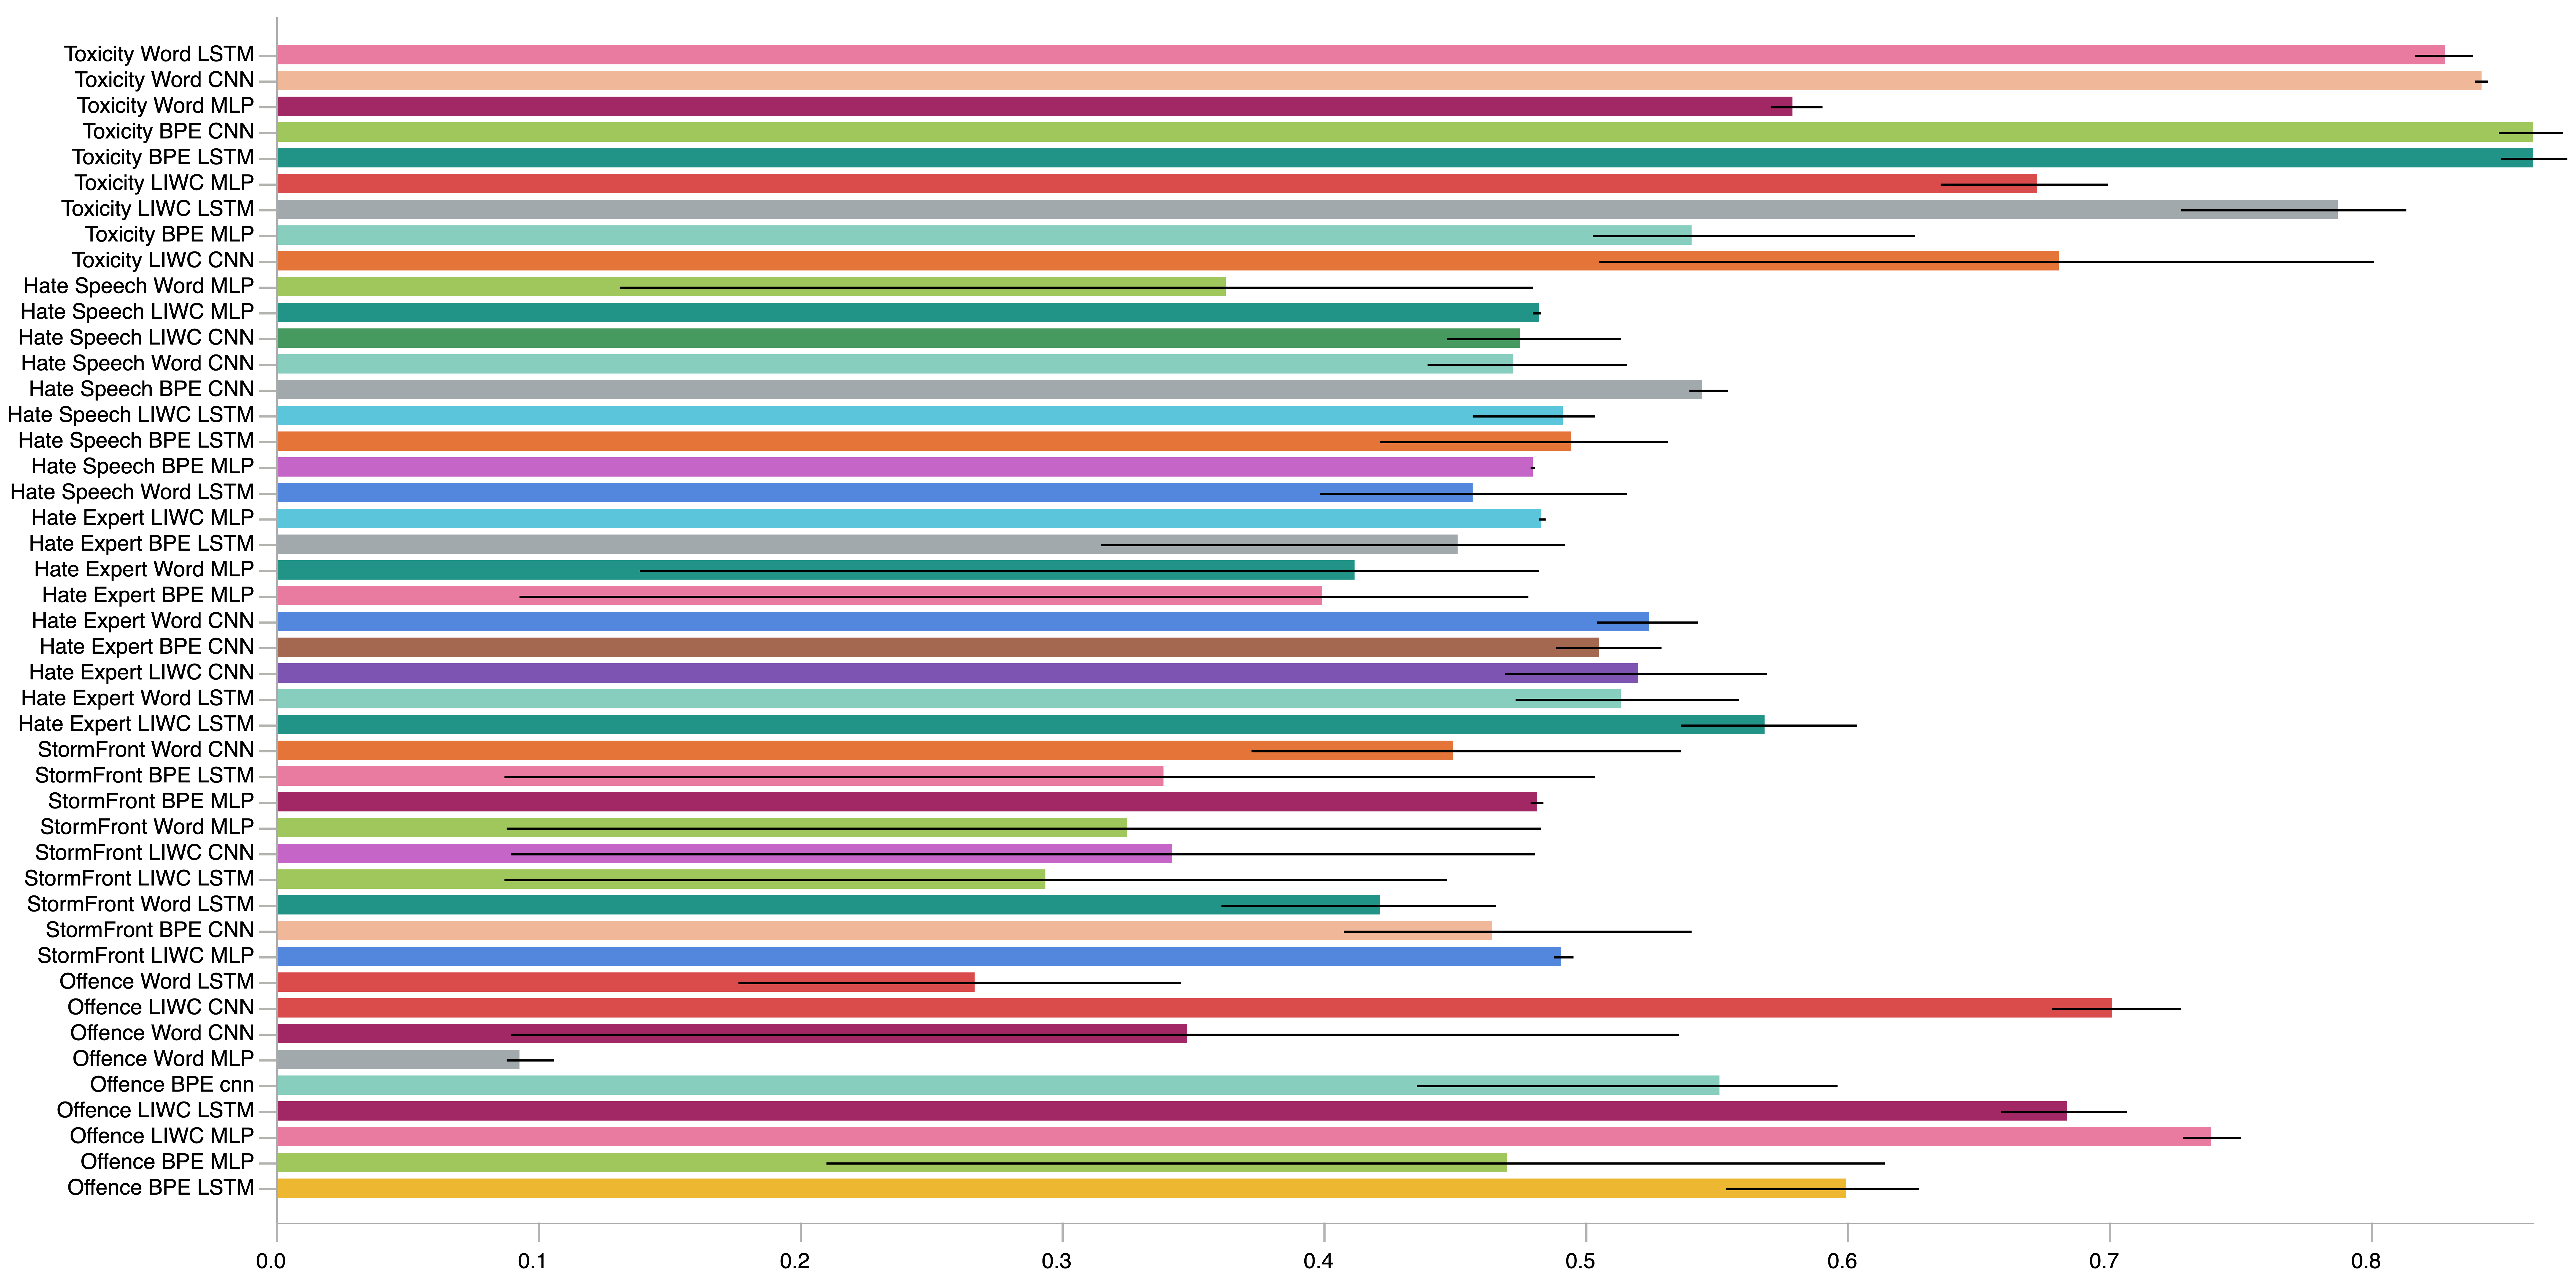
\includegraphics[width=0.7\paperheight]{all_models_test_wulczyn.png}
  \caption{Macro F1 scores for models on the \textit{Toxicity} test set with the standard deviation represented in error bars.}
  \label{fig:wulczyn_models_test}
\end{figure}

\begin{figure}
  \includegraphics[width=0.7\paperheight]{all_models_test_waseem.png}
  \caption{Macro F1 scores for models on the \textit{Hate Expert} test set with the standard deviation represented in error bars.}
  \label{fig:waseem_models_test}
\end{figure}

\begin{figure}
  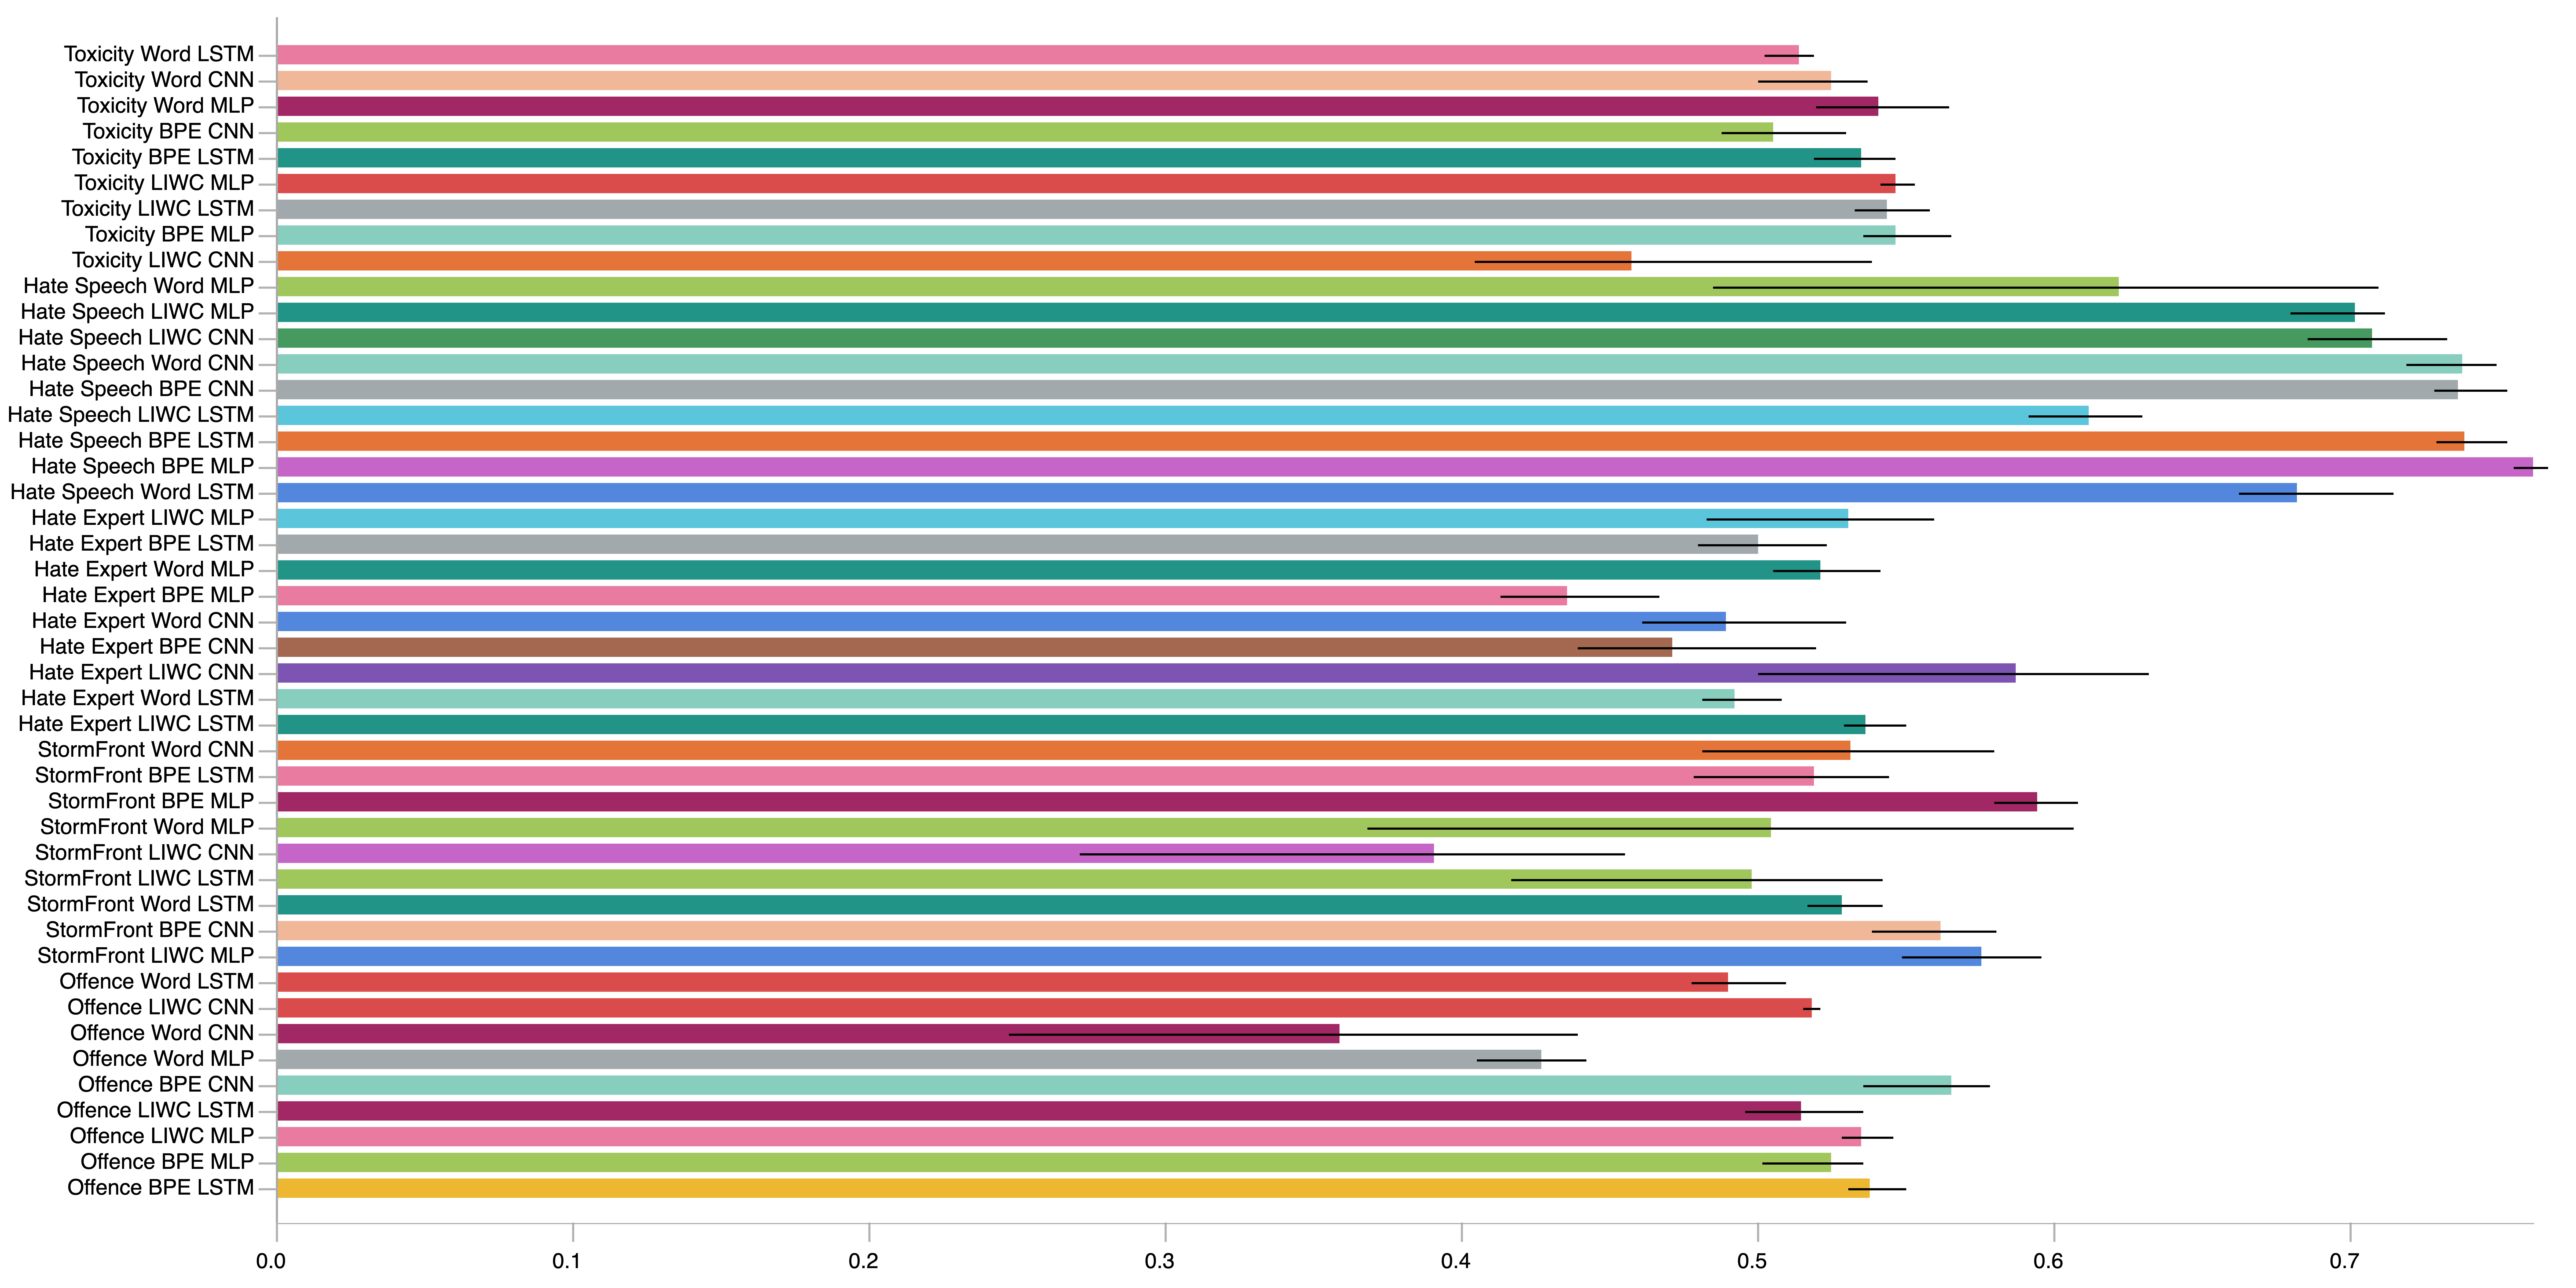
\includegraphics[width=0.7\paperheight,height=\textwidth]{all_models_test_waseem_hovy.png}
  \caption{Macro F1 scores for models on the \textit{Hate Speech} test set with the standard deviation represented in error bars.}
  \label{fig:waseem_hovy_models_test}
\end{figure}

\begin{figure}
  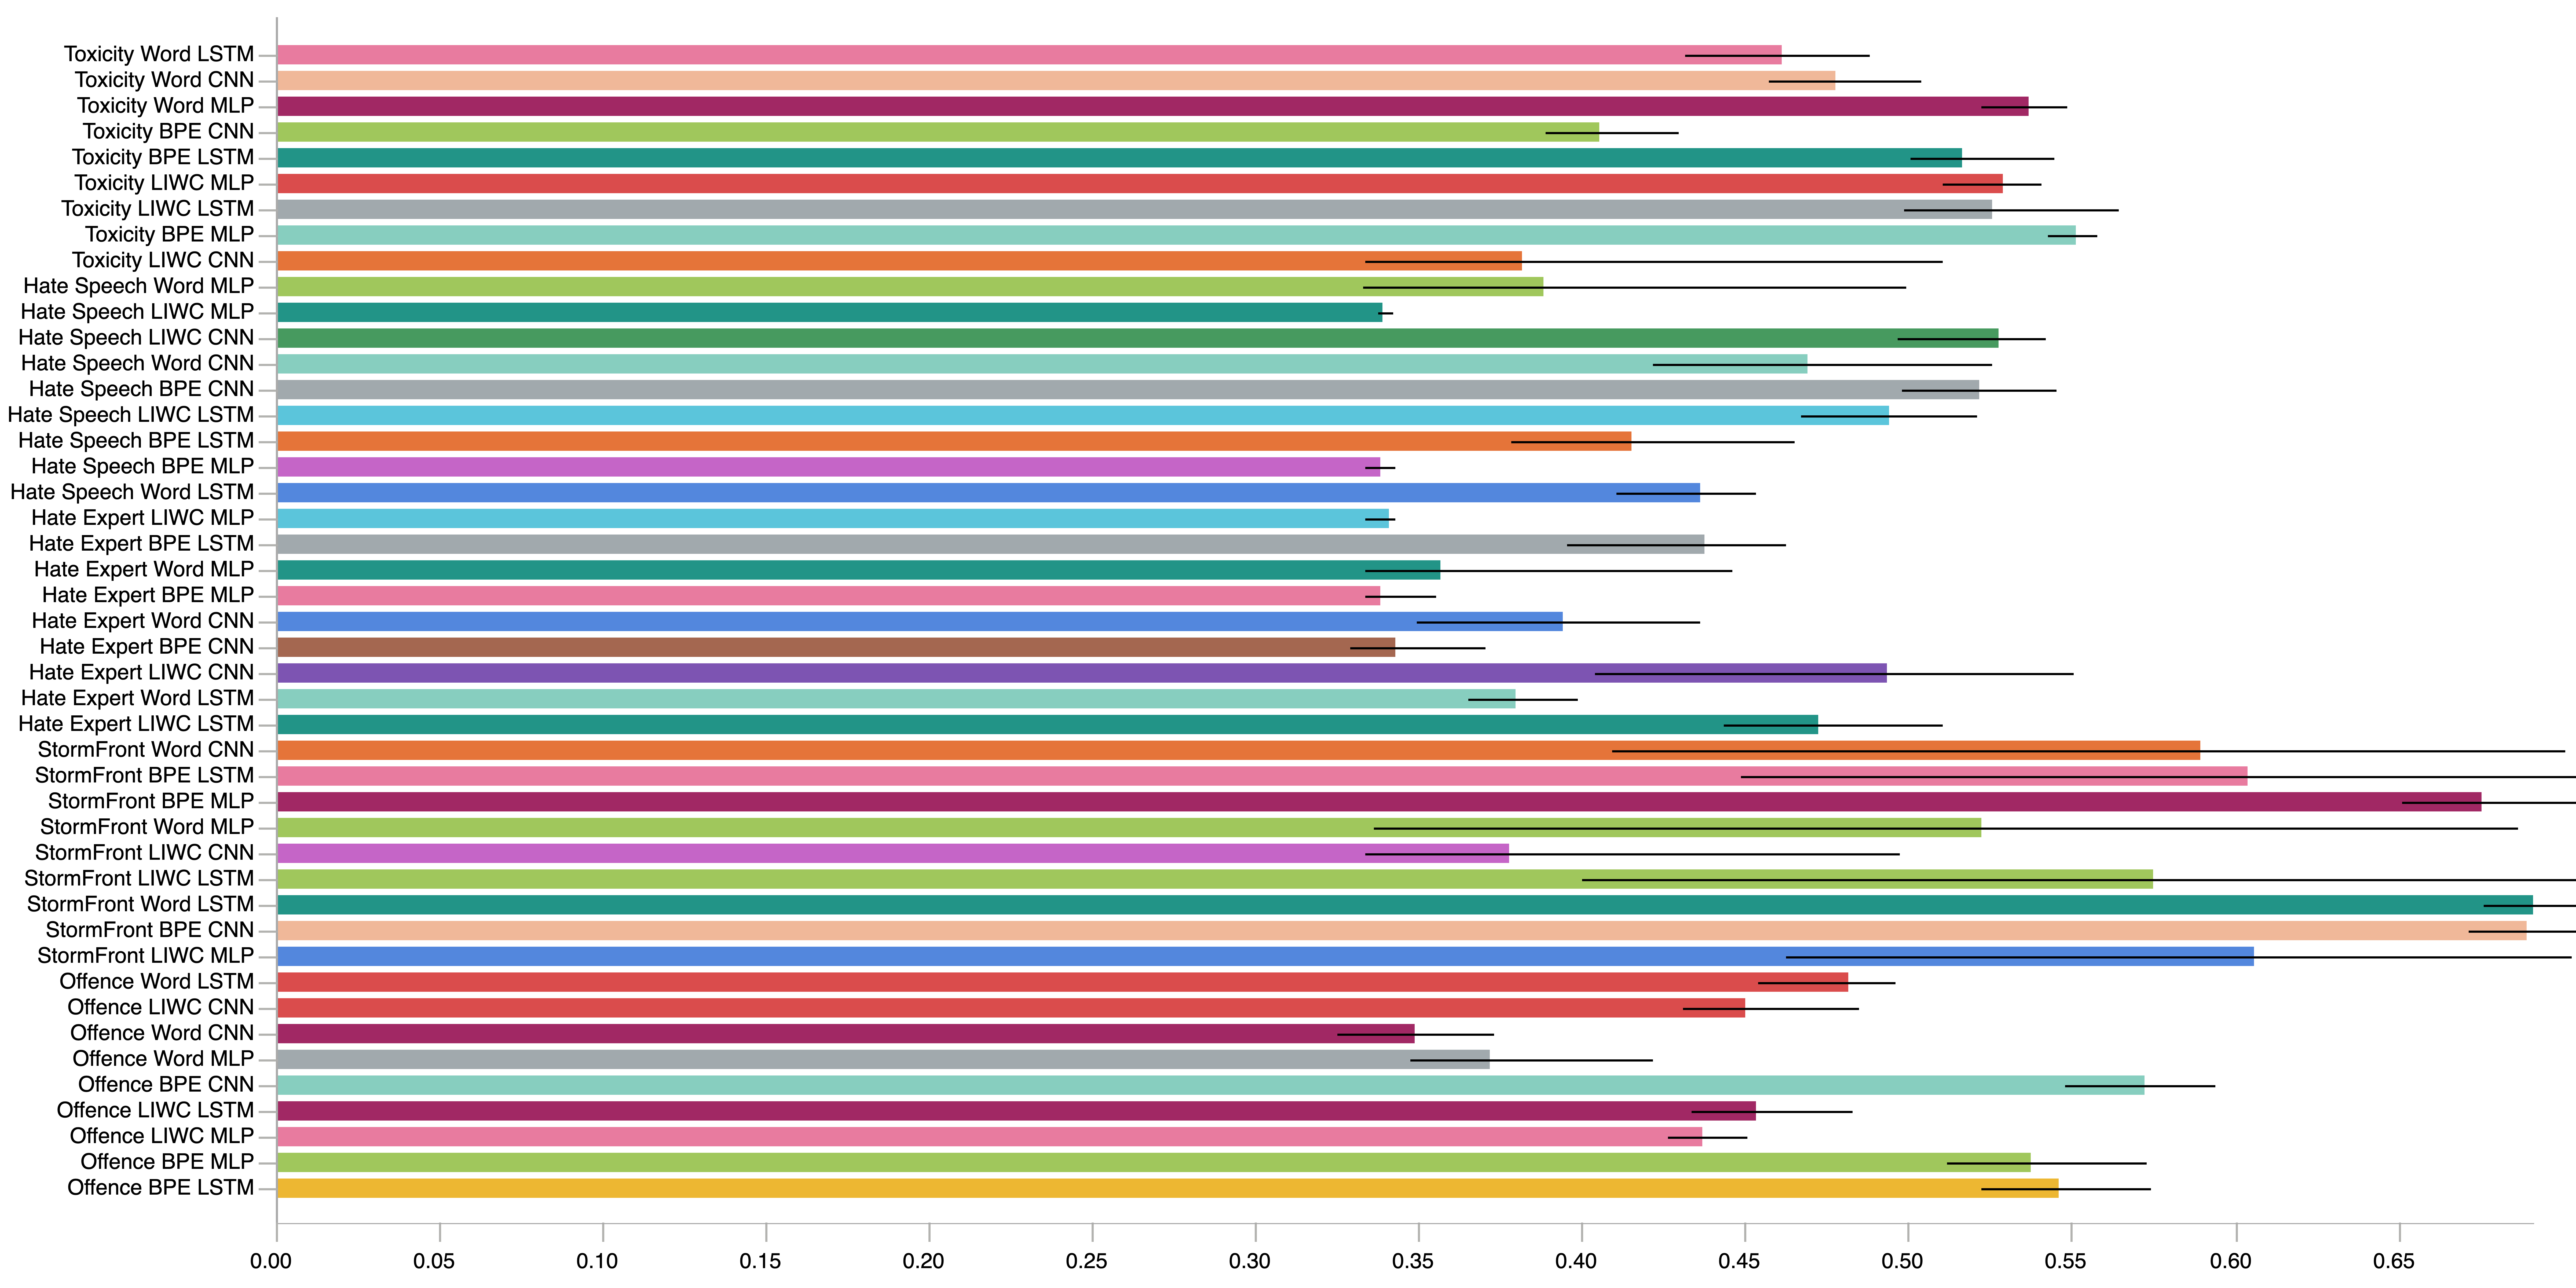
\includegraphics[width=0.7\paperheight]{all_models_test_garcia.png}
  \caption{Macro F1 scores for models on the \textit{StormFront} test set with the standard deviation represented in error bars.}
  \label{fig:waseem_hovy_models_test}
\end{figure}
\end{landscape}

\zw{UPDATE: Change F1, Accuracy, precision, recall names to full names from acc, prec, rec}
\begin{landscape}
\begin{table}[]
\centering
\resizebox{1.4\textheight}{!}{%
\begin{tabular}{ccl|llll|llll|llll|llll|llll}
                                     &                         &                                & \multicolumn{4}{c|}{Davidson} & \multicolumn{4}{c}{Wulczyn}   & \multicolumn{4}{c}{Waseem}    & \multicolumn{4}{c}{Waseem-Hovy} & \multicolumn{4}{c}{Garcia} \\
 Training data                       & Representation          & Model                          & F1    & acc    & prec & rec   & F1    & acc   & prec  & rec   & F1    & acc   & prec  & rec   & F1    & acc   & prec  & rec     & F1    & acc    & prec & rec   \\ \hline
\multirow{12}{*}{\rot{Davidson}}     & \mrow{6}{*}{\rot{BPE}}  & Support Vector Machine         &$92.19$&$95.60$&$91.91$&$92.47$&$71.26$&$86.83$&$67.87$&$92.47$&$49.06$&$68.64$&$49.56$&$49.41$&$58.49$&$65.66$&$49.41$&$58.25$  &$60.62$&$60.66$&$60.71$&$60.66$\\
                                     &                         & Logistic Regression            &$91.39$&$95.19$&$91.51$&$91.27$&$71.18$&$86.40$&$67.68$&$79.85$&$48.34$&$66.04$&$49.35$&$49.03$&$58.12$&$64.36$&$58.37$&$57.98$  &$58.15$&$58.15$&$58.16$&$58.15$\\
                                     &                         & Multi-Layered Perceptron       &$     $&$     $&$     $&$     $&$     $&$     $&$     $&$     $&$     $&$     $&$     $&$     $&$     $&$     $&$     $&$     $  &$     $&$     $&$     $&$     $\\
                                     &                         & Convolutional Neural Network   &$     $&$     $&$     $&$     $&$     $&$     $&$     $&$     $&$     $&$     $&$     $&$     $&$     $&$     $&$     $&$     $  &$     $&$     $&$     $&$     $\\
                                     &                         & Long-Short Term Memory network &$     $&$     $&$     $&$     $&$     $&$     $&$     $&$     $&$     $&$     $&$     $&$     $&$     $&$     $&$     $&$     $  &$     $&$     $&$     $&$     $\\
                                     & \mrow{6}{*}{\rot{LIWC}} & Support Vector Machine         &$86.85$&$92.01$&$84.41$&$90.12$&$75.32$&$90.02$&$72.41$&$79.78$&$53.29$&$71.24$&$53.27$&$54.42$&$55.89$&$65.36$&$57.59$&$55.93$  &$44.92$&$49.58$&$49.36$&$49.58$\\
                                     &                         & Logistic Regression            &$87.19$&$92.41$&$85.37$&$89.41$&$74.91$&$89.69$&$71.85$&$79.81$&$51.90$&$68.78$&$52.30$&$53.36$&$56.43$&$64.83$&$57.51$&$56.32$  &$45.23$&$48.74$&$48.31$&$48.74$\\
                                     &                         & Multi-Layered Perceptron       &$     $&$     $&$     $&$     $&$     $&$     $&$     $&$     $&$     $&$     $&$     $&$     $&$     $&$     $&$     $&$     $  &$     $&$     $&$     $&$     $\\
                                     &                         & Convolutional Neural Network   &$     $&$     $&$     $&$     $&$     $&$     $&$     $&$     $&$     $&$     $&$     $&$     $&$     $&$     $&$     $&$     $  &$     $&$     $&$     $&$     $\\
                                     &                         & Long-Short Term Memory network &$     $&$     $&$     $&$     $&$     $&$     $&$     $&$     $&$     $&$     $&$     $&$     $&$     $&$     $&$     $&$     $  &$     $&$     $&$     $&$     $\\\hline

\mrow{12}{*}{\rot{Wulczyn}}          & \mrow{6}{*}{\rot{BPE}}  & Support Vector Machine         &$63.89$&$70.55$&$66.24$&$78.47$&$86.42$&$95.59$&$89.11$&$84.15$&$53.45$&$80.34$&$55.30$&$53.23$&$51.95$&$67.90$&$59.86$&$54.19$  &$52.89$&$58.99$&$68.66$&$58.99$\\
                                     &                         & Logistic Regression            &$59.86$&$64.30$&$64.25$&$75.47$&$86.24$&$95.63$&$89.94$&$83.31$&$51.22$&$80.92$&$53.43$&$51.64$&$50.56$&$68.14$&$60.38$&$53.64$  &$50.04$&$57.53$&$68.78$&$57.53$\\
                                     &                         & Multi-Layered Perceptron       &$     $&$     $&$     $&$     $&$     $&$     $&$     $&$     $&$     $&$     $&$     $&$     $&$     $&$     $&$     $&$     $  &$     $&$     $&$     $&$     $\\
                                     &                         & Convolutional Neural Network   &$     $&$     $&$     $&$     $&$     $&$     $&$     $&$     $&$     $&$     $&$     $&$     $&$     $&$     $&$     $&$     $  &$     $&$     $&$     $&$     $\\
                                     &                         & Long-Short Term Memory network &$     $&$     $&$     $&$     $&$     $&$     $&$     $&$     $&$     $&$     $&$     $&$     $&$     $&$     $&$     $&$     $  &$     $&$     $&$     $&$     $\\
                                     & \mrow{6}{*}{\rot{LIWC}} & Support Vector Machine         &$76.06$&$81.72$&$73.73$&$88.34$&$83.20$&$95.05$&$90.72$&$78.42$&$54.49$&$82.51$&$59.19$&$54.12$&$49.82$&$68.02$&$59.77$&$53.23$  &$39.70$&$51.67$&$58.13$&$51.67$\\
                                     &                         & Logistic Regression            &$72.62$&$78.17$&$71.52$&$86.30$&$82.67$&$94.95$&$90.88$&$77.65$&$54.26$&$82.94$&$59.99$&$53.99$&$49.11$&$67.78$&$58.88$&$52.81$  &$39.41$&$51.67$&$58.77$&$51.67$\\
                                     &                         & Multi-Layered Perceptron       &$     $&$     $&$     $&$     $&$     $&$     $&$     $&$     $&$     $&$     $&$     $&$     $&$     $&$     $&$     $&$     $  &$     $&$     $&$     $&$     $\\
                                     &                         & Convolutional Neural Network   &$     $&$     $&$     $&$     $&$     $&$     $&$     $&$     $&$     $&$     $&$     $&$     $&$     $&$     $&$     $&$     $  &$     $&$     $&$     $&$     $\\
                                     &                         & Long-Short Term Memory network &$     $&$     $&$     $&$     $&$     $&$     $&$     $&$     $&$     $&$     $&$     $&$     $&$     $&$     $&$     $&$     $  &$     $&$     $&$     $&$     $
\end{tabular}%
}
\caption{Performance of linear baseline models and index-encoded models across in-domain and out-of-domain evaluation sets.}
\label{tab:redux_embedding_davidson}
\end{table}
\end{landscape}

\begin{landscape}
\begin{table}[]
\centering
\resizebox{1.4\textheight}{!}{%
\begin{tabular}{ccl|llll|llll|llll|llll|llll}
                                     &                         &                                 & \multicolumn{4}{c|}{Davidson} & \multicolumn{4}{c}{Wulczyn} & \multicolumn{4}{c}{Waseem} & \multicolumn{4}{c}{Waseem-Hovy} & \multicolumn{4}{c}{Garcia} \\
 Training data                       & Representation          & Model                           & F1 & acc & prec & rec         & F1 & acc & prec & rec       & F1 & acc & prec & rec      & F1 & acc & prec & rec           & F1 & acc & prec & rec      \\ \hline
\mrow{12}{*}{\rot{Davidson}}         & \mrow{6}{*}{\rot{BPE}}  & \textit{Support Vector Machine} &    &     &      &             &    &     &      &           &    &     &      &          &    &     &      &               &    &     &      &          \\
                                     &                         & \textit{Logistic Regression}    &    &     &      &             &    &     &      &           &    &     &      &          &    &     &      &               &    &     &      &          \\
                                     &                         & Multi-Layered Perceptron        &    &     &      &             &    &     &      &           &    &     &      &          &    &     &      &               &    &     &      &          \\
                                     &                         & Convolutional Neural Network    &    &     &      &             &    &     &      &           &    &     &      &          &    &     &      &               &    &     &      &          \\
                                     &                         & Long-Short Term Memory network  &    &     &      &             &    &     &      &           &    &     &      &          &    &     &      &               &    &     &      &          \\
                                     & \mrow{6}{*}{\rot{LIWC}} & \textit{Support Vector Machine} &    &     &      &             &    &     &      &           &    &     &      &          &    &     &      &               &    &     &      &          \\
                                     &                         & \textit{Logistic Regression}    &    &     &      &             &    &     &      &           &    &     &      &          &    &     &      &               &    &     &      &          \\
                                     &                         & Multi-Layered Perceptron        &    &     &      &             &    &     &      &           &    &     &      &          &    &     &      &               &    &     &      &          \\
                                     &                         & Convolutional Neural Network    &    &     &      &             &    &     &      &           &    &     &      &          &    &     &      &               &    &     &      &          \\
                                     &                         & Long-Short Term Memory network  &    &     &      &             &    &     &      &           &    &     &      &          &    &     &      &               &    &     &      &          \\\hline

\mrow{12}{*}{\rot{Wulczyn}}          & \mrow{6}{*}{\rot{BPE}}  & \textit{Support Vector Machine} &    &     &      &             &    &     &      &           &    &     &      &          &    &     &      &               &    &     &      &          \\
                                     &                         & \textit{Logistic Regression}    &    &     &      &             &    &     &      &           &    &     &      &          &    &     &      &               &    &     &      &          \\
                                     &                         & Multi-Layered Perceptron        &    &     &      &             &    &     &      &           &    &     &      &          &    &     &      &               &    &     &      &          \\
                                     &                         & Convolutional Neural Network    &    &     &      &             &    &     &      &           &    &     &      &          &    &     &      &               &    &     &      &          \\
                                     &                         & Long-Short Term Memory network  &    &     &      &             &    &     &      &           &    &     &      &          &    &     &      &               &    &     &      &          \\
                                     & \mrow{6}{*}{\rot{LIWC}} & \textit{Support Vector Machine} &    &     &      &             &    &     &      &           &    &     &      &          &    &     &      &               &    &     &      &          \\
                                     &                         & \textit{Logistic Regression}    &    &     &      &             &    &     &      &           &    &     &      &          &    &     &      &               &    &     &      &          \\
                                     &                         & Multi-Layered Perceptron        &    &     &      &             &    &     &      &           &    &     &      &          &    &     &      &               &    &     &      &          \\
                                     &                         & Convolutional Neural Network    &    &     &      &             &    &     &      &           &    &     &      &          &    &     &      &               &    &     &      &          \\
                                     &                         & Long-Short Term Memory network  &    &     &      &             &    &     &      &           &    &     &      &          &    &     &      &               &    &     &      &          \\
\end{tabular}%
}
\caption{Performance of onehot-encoded models across in-domain and out-of-domain datasets (\textit{italic} denotes baseline models).}
\label{tab:redux_embedding_davidson}
\end{table}
\end{landscape}
\zw{Add results and start by rough analysis of just numbers}
\zw{Add plots for development of loss over each epoch}
\zw{Add plots for F1 score during the evaluation set}
\zw{Look at predictions in detail, try to identify where they still fail}
\zw{Do logistic regression and to find out what clear patterns there are}

While the onehot and index encoded tensors should functionally be equal to one another, we see a direct influence of the input layers on the classification scores; with all models showing stronger performance using linear input layers. We propose that the reason for such discrepancies lie in the simpler training procedure of linear layers which don't seek to find relationships between different tokens but instead simply provide a linear function, and embedding layers that seek to identify the relationships between each all tokens in the dataset.

\section{Conclusions and future work}

\zw{Something about BERT based models}
BERT \cite{Koufakou,Vidgen,Tran:2020,Isaksen:2020}
As our aim is to consider the influence of LIWC-represented documents, we do not consider the more recent pre-trained Transformer-based language models \citep[e.g.]{Devlin:2019,Liu:2019} as the amounts of data necessary to train such a masked language model with LIWC representations are unavailable. Moreover, as the LIWC dictionary only occupies a small fraction of the entire English lexicon, and its tokens are abstractions on use of the language, training a language model is a fruitless endeavour.

\zw{Something about pretrained embedding layer + training liwc embedding layer}

\zw{Some concluding remarks}
While functionally this limits the vocabulary, there is also loss of information. Future work, could then employ both simple and complex mappings of different forms of words to single tokens that cohere with the LIWC dictionary, thus limiting information loss while retaining the predictive power.

\subsection{Limitations}
Although such lack of recognition can have positive effects, such as lower false positive rate, the politics of not being recognised, as argued by \citet{Benjamin:2019} are not straightforward and the lack of recognition does not provide a guarantee that systemic harm will not occur. For instance, if systems developed to detect abuse did not recognise Multi-cultural London English due to vocabulary reductions, any abuse that was written in that dialect would not be recognised, leaving those users in harms way. Given that LIWC was developed using ``dictionaries, thesauruses, questionnaires, and lists made by research assistants'' \citep{Tauscik:2010} in a North American context, it is highly unlikely that word forms that differ from mainstream usage were included. For instance, the commonly used `brotha' and `bruva' in North American and British contexts, respectively, are absent from the dictionary.

% **************************** Define Graphics Path **************************
\ifpdf
    \graphicspath{{Chapter5/Figs/Raster/}{Chapter5/Figs/PDF/}{Chapter5/Figs/}}
\else
    \graphicspath{{Chapter5/Figs/Vector/}{Chapter5/Figs/}}
\fi

\chapter{LIWC/text transformation chapter}\label{chap:liwc}

\zw{Describe problem field}
One of the key issues in machine learning for content moderation is that such systems both in deployed settings (see \autoref{chap:filter}) and in research (see \autoref{chap:intro} and \autoref{chap:nlp}) over-fit to individual tokens that see over-representation in the positive and negative classes respectively. While research efforts have been made to address such issues \cite{CITE: cite papers that try to address overfitting}, the problem of over-fitting to words and identity markers remain an open question for the field. While some such approaches have addressed this problem by replacing certain words and phrases with more general tokens \cite{CITE: Replacing token papers} or masking \cite{CITE: Masking token paper} tokens. Other work has attempted to address the problem by treating it as a problem of dataset bias \cite{CITE: Bias papers}. Here we instead we propose a different approach which serves multiple purposes of 1) minimising the vocabulary to avoid over-fitting to distributional skews in vocabulary across classes; 2) representing documents in terms of how they represent thoughts, feelings, personality, and motivations \cite{LIWC:2015}; and 3) returning modelling of hate speech and different forms of abuse to simpler dictionary-lookup methods that simplify modelling of abuse to how words are used, rather than focusing on their surface forms, to achieve similar performance as compared to more complex models.

Through the use of the Linguistic Inquiry and Word Count (LIWC) dictionary, we transform documents from large vocabularies, that are riddled with typos, spelling mistakes, and obfuscations to the functions how these words are used. As seen in \autoref{fig:liwc_transform}, the transformation of words to LIWC categories both contain deeper information about how words are used, and encode a loss of information in words that do not exist in the LIWC dictionary. However, by radically reducing the sizes of vocabularies, from several thousand unique tokens to around 1000 unique tokens that provide deeper insights than simply selecting the most frequent tokens. Moreover we show that the strength of the classification performances within the dataset will translate to other datasets, as these transformed tokens are more general than their surface form.

Focusing our attentions on simple deep neural networks and shallow models, we show that by radically reducing the vocabulary size, while increasing the contextual information of the remaining vocabulary, we can achieve strong classification performances within datasets and more importantly, on out of domain datasets.

\zw{Provide example of transformation}
\section{Previous work}

\zw{Talk about LIWC: Designed for long form documents}


\zw{Talk about LIWC}
\zw{Talk in depth about the references from \autoref{chap:nlp}.}

\subsection{Datasets}
Beyond the different specific models and types of input layer, the datasets themselves also differ strongly from one another across a number of attributes: the various sizes of the datasets, the platforms the datasets have been sampled from, the annotator selection, the annotation guidelines, and the aims of the datasets. As we seek to build generalisable models and compare the performance across datasets, we reduce the classification task in each dataset to a binary `abuse/not-abuse' class, as each dataset addresses different aspects and notions of abuse.
We train our models on either the Twitter dataset collected by \citet{Davidson:2017} or the Wikipedia Talk pages dataset sampled by \citet{Wulczyn:2017} as our training datasets, in part due to the sizes of the datasets and in part due to the different breadth of communicative styles. To estimate cross-dataset performance, we evaluate our models on \citet{Waseem-Hovy:2016}, \citet{Waseem:2016}, and \citet{Garcia:2019}.

\zw{INSERT: Table of BPE and LIWC vocabularies}
\zw{INSERT: Short paragraph on vocabularies.}

\subsubsection{Training Datasets}
Our first dataset for training is the dataset developed by \citet{Davidson:2017} consists of $24,784$ tweets that are sampled from Twitter using keywords obtained from \citet{Hatebase}. The dataset is annotated for ``hate speech'', ``offensive language'' and ``neither''. The collection rationale was that not all content that immediately appears to be abusive is necessarily that, and that hate speech models must be able to distinguish between what is offensive and what is hateful \cite{Davidson:2017} (please see \autoref{chap:nlp} and \autoref{chap:filter} for more in-depth discussions on the implications of label categories, their overlap and differences). The dataset was annotated by crowd-workers on FigureEight\footnote{Previously known as CrowdFlower}. Unlike most datasets for abuse, this dataset consists primarily of positive instances, with $77$\% of the (binarised) dataset belonging to the positive class.

Our second dataset used for training is the dataset presented by \citet{Wulczyn:2017}. This dataset consists of more then $100,000$ comments from Wikipedia talk pages that have been annotated for personal attacks and toxicity \cite{Wulczyn:2017}. The rationale of this dataset is that personal attacks are harmful to ongoing conversations, and that through the identification and removals of comments that poison, or toxify online conversations, more space will be left for healthy and constructive discussions (please see \autoref{chap:filter} for an in-depth consideration of the politics of what constitutes ``toxic'' and ``healthy''). The binarised distribution of documents tagged for toxicity aligns better with prior research, with the positive class consuming $\approx 9$\% of the dataset.

\subsubsection{Evaluation Datasets}
For our evaluation datasets, we use \citet{Waseem-Hovy:2016}, a dataset of $16,000$ documents that are sampled from Twitter and annotated for ``racism'', ``sexism'', and ``neither''. The dataset was annotated by two coders, who labelled $31$\% of the dataset containing as either ``sexist'' or ``racist'' content. This dataset was developed for an early exploration into automated content moderation of online hate speech. We also use the dataset by \citet{Waseem:2016} that followed this first exploration. Here the annotation guidelines remain the same while the label-set is expanded to include the intersection of racism and sexism, the ``both'' category. This dataset contains $6000$ documents, labelled by intersectional feminist activists, and another label-set annotated by crowd-workers from FigureEight. We choose the intersectional feminist tagged annotations, as \citet{Waseem:2016} show that simple computational models perform better using this tagset. The binarised positive labels occupy $15.19$\% of the dataset. Finally, we use the dataset on white-supremacist speech developed by \citet{Garcia:2019}. This dataset, unlike the previous two evaluation datasets does not stem from Twitter, but instead the data is collected from StormFront\footnote{www.stormfront.net}, a web forum dedicated to the preservation and dissemination of white supremacist ideology. This dataset contains \zw{INSERT: Number of total document counts when using the entire dataset instead of the balanced one.} documents labelled for being hateful or not hateful, with \zw{INSERT: Percentage of positive class docs} in the positive class.

\subsubsection{Dataset and Platform Affordances}

As the datasets differ quite significantly in the sizes of the raw number of documents as well as the vocabulary sizes. Moreover, as the datasets are selected from different websites with different communities, purposes, and means of interaction; the data sampled from each platform may differ in content as well as style. Considering for instance \citet{Waseem:2016}, this dataset was collected on Twitter while the maximum length of a tweet was $140$ characters. Documents are thus short as they are given an upper limit on the number of characters. On the other hand, \citet{Wulczyn:2017} collected their data from the Wikipedia Editor Talk pages, where comments are not limited by length. Additionally, these two domains differ in that conversations on Twitter may have no particular topic, conversations on Wikipedia Talk pages always refer back to a specific topic and the conversation of how to address a particular edit to a page. Finally, given Wikipedia's ongoing issues with recruiting editors from a diverse set of backgrounds \cite{CITE: Wikipedia editors issue} and Twitter's comparatively broad user base \cite{CITE: Twitter userbase by demographic ref} may influence which dialects are represented on the platforms, which patterns of speech (e.g. sociolects, slang, and shorthand) occur, and the style of the discussions and conversations.

\subsubsection{Annotator Selection}

There are some interesting discrepancies in the selection of annotators for the datasets that we apply our models to. \citet{Waseem:2016} select their annotators based on socio-political positions, controlling for a specific interpretation of abuse. On the other hand \citet{Wulczyn:2017} select their annotators from the users of the Wikipedia Talk pages. However, the Wikipedia editor community has been accused of being a highly male space that is unwelcoming to women \cite{CITE: Cite article talking about anti-women culture on wikipedia}. This suggests that the influence of their selection of annotators, who are culturally situated in the norms and culture of the Wikipedia editor community, are also likely to be less attuned to content that may be offensive to women, but is accepted communicative practices within the Wikipedia editor community.

On the other hand \citet{Garcia:2019} and \citet{Davidson:2017} select annotators that are removed from the context of the documents they are annotating. This suggests that global understandings of what constitutes abuse are possible, and that it is possible to annotate without a deep understanding of the issues and communicative practices of the specific communities that are being investigated.

While we accept that the influence of annotation guidelines have strong influences on the subject that is being examined (e.g. \citet{Davidson:2017} examine the differences in what is merely offensive and what is hateful, \citet{Garcia:2019} examine what is hateful from a white supremacist community and what is not, and \citet{Wulczyn:2017} examine things that make conversations toxic and hostile), we assume that these different guidelines and questions highlight different aspects of abuse. Through our efforts to develop methods that can identify different forms of abuse across different datasets, we accept the assumption that there are some global understandings of abuse that can be learned by machine learning models. We revisit this assumption in \autoref{chap:disembodied}.

\section{Modelling}

\subsection{Neural Models}\ref{sec:redux_neural}

We implement and train four different model architectures with two variations each, resulting in a total of 8 different neural models for each input representation. We choose to train a Multi-Layered Perceptron, a Recurrent Neural Network, a Long-Short Term Memory network, and a Convolutional Neural Network. We choose these four models as they have each been used in previous work \cite{CITE: Find papers with Neural approaches for each of the models}. Each of the four models are trained with either a linear input layer and an embedding input layer. We choose to make this distinction as our datasets are too small to meaningfully learn embedding layers, yet for the LIWC transformed documents, pre-trained embeddings have little value, as all tokens would be out-of-vocabulary. Thus to compare comparable entities, we train a model with each type of input layer. This difference in the input layers however also implies a difference in how each document is represented: for the models with linear input layers, each document is encoded as a onehot tensor whereas the models that use an embedding layer as it's input layer the documents are represented as index-encoded tensors (please see \autoref{fig:onehot_embedding} for an illustration). For all neural models, we use gradient clipping to prevent the issue of exploding gradients \cite{Bengio:1994}. All neural models are implemented using PyTorch \cite{CITE: Pytorch paper}.

\begin{figure}
  \centering
  \includegraphics[scale=0.75]{onehot_embedding.jpg}
  \caption{Onehot and Index encoded tensors.}
  \label{fig:onehot_embedding}
\end{figure}

In order to focus on the utility of the transformed document representations, we use bare bones models with simple architectures. To address the issue of the models over-fitting to the data either by identifying spurious correlations or by over-training the model, we subject each model to dropout and early stopping criteria (please see \autoref{sec:dropoutearly} for more details on the functionality of early stopping and dropout).

We perform Bayesian Hyper Parameter Tuning using Weights and Biases \cite{Wandb} to identify the optimal parameters for each model and the variants of each model, evaluated using macro-F1 score. We also investigate the influence of batch sizes and learning rate. For more in depth explanation of how each model works, please refer to \autoref{sec:model_background}.\vspace{5mm}

\begin{landscape}
\begin{table}[]
\centering
\begin{tabular}{lllllllll}
                      & \multicolumn{4}{c}{BPE}                 & \multicolumn{4}{c|}{LIWC} \\
                       & MLP     & CNN      & RNN     & LSTM    & MLP     & CNN     & RNN     & LSTM     \\ \hline
Embedding Dimension    & $100$   & $300$    & $100$   & $300$   & $100$   & $100$   & $100$   & $100$    \\
Hidden Dimension       & $300$   & $64$     & $300$   & $300$   & $300$   & $100$   & $300$   & $100$    \\
Window Size            & -       & $2, 3 4$ & -       & -       & -       & -       & -       & -        \\
Batch Size             & $16$    & $32$     & $16$    & $64$    & $16$    & $64$    & $64$    & $64$     \\
Learning Rate          & $0.001$ & $0.001$  & $0.01$  & $0.001$ & $0.001$ & $0.001$ & $0.001$ & $0.001$  \\
Dropout                & $0.2$   & $0.2$    & $0.0$   & $0.1$   & $0.1$   & $0.0$   & $0.0$   & $0.0$    \\
Activation Function    & Tanh    & Tanh     & Tanh    & Tanh    & ReLU    & ReLU    & Tanh    & Tanh     \\
# Epochs               & $100$   & $50$     & $50$    & $100$   & $200$   & $50$    & $100$   & $200$    \\
Validation F1-score    & $84.24$ & $85.10$  & $45.41$ & $72.01$ & $87.54$ & $86.01$ & $43.73$ & $82.67$  
\end{tabular}
\caption{Best hyper-parameter setting for neural models with embedding input layer trained on \citet{Davidson:2017}.}
\label{tab:redux_hyperparam_search_davidson}
\end{table}
\end{landscape}


\begin{landscape}
\begin{table}[]
\centering
\begin{tabular}{lllllllll}
                      & \multicolumn{4}{c}{BPE}               & \multicolumn{4}{c|}{LIWC} \\
                      & MLP     & CNN     & RNN     & LSTM    & MLP     & CNN     & RNN     & LSTM    \\ \hline
Embedding Dimension   & $100$   &         &         &         & $300$   &         &         &         \\
Hidden Dimension      & $300$   &         &         &         & $300$   &         &         &         \\
Window Size           & -       &         &         &         & -       &         &         &         \\
Batch Size            & $32$    &         &         &         & $32$    &         &         &         \\        
Learning Rate         & $0.001$ &         &         &         & $0.001$ &         &         &         \\
Dropout               & $0.0$   &         &         &         & $0.1$   &         &         &         \\
Activation Function   & ReLU    &         &         &         & Tanh    &         &         &         \\
# Epochs              & $50$    &         &         &         & $200$   &         &         &         \\
Validation F1-score   & $82.39$ &         &         &         & $82.90$ &         &         &
\end{tabular}
\caption{Best hyper-parameter setting for neural models with embedding input layer trained on \citet{Wulczyn:2017}.}
\label{tab:redux_hyperparam_search_wulczyn}
\end{table}
\end{landscape}


\subsubsection{Multi-Layered Perceptron}

The first neural model that we use, is a Multi-Layered Perceptron. We choose the model as it is a simple neural network, that can act as a minimal setting of the usefulness of neural networks. Our Multi-Layered Perceptron consists of either a linear input layer or an embedding input layer. The obtained representation of a batch of documents are then passed on to a linear hidden layer and passed on to a linear output layer, which is subject to a softmax layer computing probability estimates for each class. Following the first and second layer of the model architecture, we subject the output of the layer to a non-linear activation function and a dropout layer. The model architecture is depicted in \autoref{fig:liwc_mlp}. For the Multi-Layered Perceptron models, we search over the following values:

\begin{itemize}
  \item Batch size: $[16, 32, 64]$,
  \item learning rate: $[0.1, 0.01, 0.001]$
  \item dropout probability: $[0.0, 0.1, 0.2]$,
  \item hidden layer dimension: $[100, 300]$, and
  \item the activation function: $[Tanh, ReLU]$
\end{itemize}

For the models that use an embedding layer as their input layers, we additionally search for the dimension of the embedding layer, allowing the model to search between $[100, 300]$. For the linear input layer model, the hidden dimension search functionally replaces the search over the embedding size.

\begin{figure}
  \centering
  \includegraphics[scale=0.75]{mlp.jpg}
  \caption{Multi-Layered Perceptron model architecture.}
  \label{fig:liwc_mlp}
\end{figure}


\subsubsection{Recurrent Neural Network}

The second neural model we implement a Recurrent Neural Network; we choose this model as it offers improvements over Multi-Layered Perceptron due to the introduction of the recurrence over the tokens in the documents (see \autoref{chap:nlp} for more detail). Our Recurrent Neural Network consists of an input layer, which can be a linear layer or an embedding layer, a recurrent neural network layer, a linear output layer, a dropout layer, and a softmax layer to compute the probabilities of each class. The recurrent neural network layer is provided an activation function, which is applied within the layer. 

The model is trained by first passing batches of index or onehot encoded documents through the input layer, and are passed on to the recurrent neural network layer.\footnote{We use the PyTorch implementation of the Recurrent Neural Network layer.} The resulting representation is then subject to a dropout layer before it subject to a linear layer that maps to the number of output classes. Finally, the softmax layer computes the probability estimates for each class. See \autoref{fig:liwc_rnn} for a depiction of the models. We set the activation function for the recurrent neural network to $\Tanh$.

For the Recurrent Neural Networks, we perform a hyper-parameter tuning over the following parameters and values:

\begin{itemize}
  \item Batch size: $[16, 32, 64]$,
  \item learning rate: $[0.1, 0.01, 0.001]$
  \item dropout probability: $[0.0, 0.1, 0.2]$,
  \item embedding layer dimension: $[100, 300]$, and
  \item hidden layer dimension: $[100, 300]$.
\end{itemize}

\begin{figure}
  \centering
  \includegraphics[scale=0.75]{rnn.jpg}
  \caption{Recurrent Neural Network model architecture.}
  \label{fig:liwc_rnn}
\end{figure}

\subsubsection{Long-Short Term Memory}

The Long-Short Term Memory network that we implement, consists of an input layer, that similarly to the RNN and MLP can be either a linear layer or an embedding layer; a one-directional Long-Short Term Memory network layer;\footnote{We use the PyTorch implementation of the Long-Short Term Memory Network layer.} an output layer; a dropout layer; and a softmax layer to compute the probabilities. The implementation of the Long-Short Term Memory layer is such that it always uses \textit{Tanh} as its non-linear activation function. We use Long-Short Term Memory networks due to their prior successes in other works \cite{CITE: LSTM papers} and because they present a development over RNNs, in that they identify information to ``forget'' in to address the issue of long-range dependencies that occur (please see \autoref{chap:nlp} for more detail).

The model is trained by passing batches of documents through the input layer prior to feeding them into the Long-Short Term Memory network layer. The output of the Long-Short Term Memory network layer is then subject to the dropout layer, before the output layer maps down to the number of label classes. Finally, the softmax layer is used to obtain an estimation of the probability distributions for each class (please see \autoref{fig:liwc_lstm} for depiction of model architecture.).

For these models, our hyper-parameter tuning considers the following parameters and values:

\begin{itemize}
  \item Batch size: $[16, 32, 64]$,
  \item learning rate: $[0.1, 0.01, 0.001]$
  \item dropout probability: $[0.0, 0.1, 0.2]$,
  \item embedding layer dimension: $[100, 300]$, and
  \item hidden layer dimension: $[100, 300]$.
\end{itemize}

\begin{figure}
  \centering
  \includegraphics[scale=0.75]{lstm.jpg}
  \caption{Long-Short Term Memory Network model architecture.}
  \label{fig:liwc_lstm}
\end{figure}

\subsubsection{Convolutional Neural Network}

For our final neural model type, we use a Convolutional Neural Network. We select this model as it has been applied previously in academic research \cite{CITE: CNN papers} and in industry (e.g. the Perspective API\footnote{https://github.com/conversationai/perspectiveapi}). Similarly to the previous model types, the input layer of the Convolutional Neural Network models can either be an embedding layer or a linear layer. The second layer of the model is a two-dimensional convolutional layer. Finally, there is an output layer and a softmax layer (See \autoref{fig:liwc_cnn} for depiction of model architecture).

For these models, we only consider the activation function, embedding, and hidden dimension in our hyper-parameter tuning, in addition to batch size and learning rate.

\begin{itemize}
  \item Batch size: $[16, 32, 64]$,
  \item learning rate: $[0.1, 0.01, 0.001]$
  \item embedding layer dimension: $[100, 300]$,
  \item hidden layer dimension: $[100, 300]$, and
  \item the activation function: $[Tanh, ReLU]$
\end{itemize}

\begin{figure}
  \centering
  \includegraphics[scale=0.75]{cnn.jpg}
  \caption{Convolutional Neural Network model architecture.}
  \label{fig:liwc_cnn}
\end{figure}

\subsection{Baseline Models}

We develop several different baseline methods to compare our method with. For each shallow baseline model (i.e. Logistic Regression and Support Vector Machines), we train two different types: a surface-token based model that uses the surface forms of the documents (e.g. words), and a LIWC based model. For each of these models, we represent each document for training and classification as a bag-of-words after removing stop words. In addition to the aforementioned models, we also train deep neural networks that similarly rely on surface forms. Specifically, we use the models described in \autoref{sec:redux_neural} providing surface level tokens as the input to the models.

\subsubsection{Baseline hyper-parameters}

Similarly to our neural models, we perform a parameter search to identify the optimal parameters for training our linear baseline models. For the Support Vector Machine models, we explore a regularisation strength of $C \in \{0.1, 0.02 \ldots 1.0\}$ and $penalty \in \{L1, L2\}$. For the Logistic Regression models, we explore the same values of $C$ and append \texttt{elasticnet} to the possible space of penalties, yielding $penalty \in \{L1, L2, elasticnet\}$. We report the optimal settings in \autoref{tab:liwc_baseline_linear_params}.

\zw{EDIT: Update this table based on binary results}

\begin{table}[]
\centering
\resizebox{\textwidth}{!}{%
\begin{tabular}{l|cccc|cccc}
                      & \multicolumn{4}{c|}{BPE}                                                             & \multicolumn{4}{c}{LIWC}                                                             \\ \hline
                      & \multicolumn{2}{c}{Logistic Regression} & \multicolumn{2}{c}{Support Vector Machine} & \multicolumn{2}{c}{Logistic Regression} & \multicolumn{2}{c}{Support Vector Machine} \\ \hline
                      & C               & Penalty               & C                 & Penalty                & C               & Penalty               & C                 & Penalty                \\ \hline
\cite{Davidson:2017}  & $1.0$           & L2                    & $0.1$             & L2                     & $0.4$           & L2                    & $0.1$             & L2                     \\
\cite{Wulczyn:2017}   & $1.0$           & L2                    & $0.2$             & L2                     & $1.0$           & L2                    & $1.0$             & L2
\end{tabular}%
}
\caption{Optimal parameters for linear Support Vector Machine baselines.}
\label{tab:liwc_baseline_linear_params}
\end{table}

Considering the performances on the in-domain during training, we see in \autoref{tab:redux_linear_baselines_dev} reasonable baseline performances on the validation set. The validation scores described in \autoref{tab:redux_linear_baselines_dev} are not as strong as the state-of-the-art in-domain models \cite{Salminen:2020}, in fact they are comparable to the scores reported on the test set of the in the original paper \cite{Davidson:2017} which provided initial baseline scores.\footnote{We do not report these baseline scores as their work does not identify which weighting of their F1-score was used.}. While several previous work augment the textual data with syntactic knowledge \cite{Davidson:2017} or advanced token representations \cite{Salminen:2020} to boost classification performance, we only use the byte-pair encoded documents and the LIWC encoded documents, to ensure comparability with our experimental models. Moreover, as our primary concern is learning classifiers whose performance generalise to other datasets, unlike much prior work which concerns itself with learning classifiers that perform well within the dataset, we do not take further steps towards boosting our baseline classifiers in-domain performances.

\begin{table}[]
\centering
\resizebox{\textwidth}{!}{%
\begin{tabular}{l|clllll}
Training data             & Document Representation                     & Model                   & F1-macro & Accuracy & Precision & Recall   \\ \hline
\multirow{4}{*}{Davidson} & \multirow{2}{*}{BPE}                        & Logistic Regression     & $92.02$  & $95.52$  & $91.82$   & $92.22$  \\
                          &                                             & Support Vector Machine  & $92.13$  & $95.56$  & $91.73$   & $92.53$  \\
                          & \multirow{2}{*}{LIWC}                       & Logistic Regression     & $87.75$  & $93.09$  & $87.43$   & $88.08$  \\
                          &                                             & Support Vector Machine  & $89.02$  & $93.62$  & $87.64$   & $90.60$  \\
\multirow{4}{*}{Wulczyn}  & \multirow{2}{*}{BPE}                        & Logistic Regression     & $86.35$  & $95.67$  & $90.04$   & $83.42$  \\
                          &                                             & Support Vector Machine  & $86.47$  & $95.50$  & $89.02$   & $84.31$  \\
                          & \multirow{2}{*}{LIWC}                       & Logistic Regression     & $82.32$  & $94.86$  & $90.48$   & $77.34$  \\
                          &                                             & Support Vector Machine  & $82.98$  & $94.96$  & $90.14$   & $78.36$
\end{tabular}%
}
\caption{In-domain scores on validation set by linear baselines.}
\label{tab:redux_linear_baselines_dev}
\end{table}

\section{Experimental Models}

To evaluate which training dataset allows for better generalisation, we train our four models described in \autoref{sec:redux_neural} and their variations on each of our training dataset, resulting in $16$ different trained models. We show the best performing model parameters on the respective validation sets in \autoref{tab:redux_hyperparam_search}. In order to gain confidence intervals, we select a subset of these models and train them with $5$ different initial random seeds, to allow us to make claims of statistical significance of our models.

We train all of our neural network models following the same training procedure. We iterate over the training dataset in multiple epochs, shuffling the order of the data at the beginning of each epoch. As we train on a single task, the loss that is propagated through the network using backpropagation is computed on the validation set for the given task. To avoid over-training our model, we implement set our models to stop training after $15$ epochs of worse, that is strictly higher, loss values. As our training procedure closes, we apply the model on each test set, allowing us to evaluate its in-domain performance as well as its out-of-domain performance.

Using this training scheme, we define and search a hyper-parameter space for each model (see \autoref{sec:redux_neural} for the search space for each model and \autoref{tab:exp_model_parameters_davidson} and \autoref{tab:exp_model_parameters_wulczyn} for the best hyper-parameters for each model). Though some previous work \cite{Waseem:2018, CITE: Other papers that restrict vocabulary sizes} limit the vocabulary that is used to train models, we make no such limitations on the surface level tokens. Instead, for all models that use surface level representations, we pre-process the documents using the 200 dimensional Byte-Pair Encoding \cite{Heinzerling:2018} for two reasons: 1) computing the sub-words allows for a minimisation of the number of out-of-vocabulary tokens and 2) computing the sub-words also minimises the sizes of the vocabularies for each dataset. For all models that take documents represented through LIWC, we dramatically reduce the vocabulary to only the tokens that exist within LIWC, setting all other tokens to a token representing that it is out-of-vocabulary.

\zw{CODING: retrain the best parameters for the models with 4 new random seeds}


\zw{Add results and start by rough analysis of just numbers}
\zw{Look at predictions in detail, try to identify where they still fail}

\begin{landscape}
\begin{table}[]
\centering
\resizebox{1.4\textheight}{!}{%
\begin{tabular}{l|clllll|}
                            & \multicolumn{6}{c}{Onehot-Encoded Models}                                                            & \multicolumn{6}{c}{Index-Encoded Models}                                                             \\
Training data               & Document Representation & Model                          & F1-macro & Accuracy & Precision & Recall  & Document Representation & Model                          & F1-macro & Accuracy & Precision & Recall  \\ \hline
\mrow{4}{*}{\rot{Davidson}} & \mrow{4}{*}{BPE}        & Multi-Layered Perceptron       &          &          &           &         & \mrow{4}{*}{BPE}        & Multi-Layered Perceptron       &          &          &           &         \\
                            &                         & Convolutional Neural Network   &          &          &           &         &                         & Convolutional Neural Network   &          &          &           &         \\
                            &                         & Long-Short Term Memory Network &          &          &           &         &                         & Long-Short Term Memory Network &          &          &           &         \\
                            &                         & Support Vector Machine         &          &          &           &         &                         & Support Vector Machine         &          &          &           &         \\
                            & \mrow{4}{*}{LIWC}       & Logistic Regression            &          &          &           &         & \mrow{4}{*}{LIWC}       & Logistic Regression            &          &          &           &         \\
                            &                         & Convolutional Neural Network   &          &          &           &         &                         & Convolutional Neural Network   &          &          &           &         \\
                            &                         & Long-Short Term Memory Network &          &          &           &         &                         & Long-Short Term Memory Network &          &          &           &         \\
                            &                         & Support Vector Machine         &          &          &           &         &                         & Support Vector Machine         &          &          &           &         \\
\mrow{4}{*}{\rot{Wulczyn}}  & \mrow{4}{*}{BPE}        & Logistic Regression            &          &          &           &         & \mrow{4}{*}{BPE}        & Logistic Regression            &          &          &           &         \\
                            &                         & Convolutional Neural Network   &          &          &           &         &                         & Convolutional Neural Network   &          &          &           &         \\
                            &                         & Long-Short Term Memory Network &          &          &           &         &                         & Long-Short Term Memory Network &          &          &           &         \\
                            &                         & Support Vector Machine         &          &          &           &         &                         & Support Vector Machine         &          &          &           &         \\
                            & \mrow{4}{*}{LIWC}       & Logistic Regression            &          &          &           &         & \mrow{4}{*}{LIWC}       & Logistic Regression            &          &          &           &         \\
                            &                         & Convolutional Neural Network   &          &          &           &         &                         & Convolutional Neural Network   &          &          &           &         \\
                            &                         & Long-Short Term Memory Network &          &          &           &         &                         & Long-Short Term Memory Network &          &          &           &         \\
                            &                         & Support Vector Machine         &          &          &           &         &                         & Support Vector Machine         &          &          &           &         \\
\end{tabular}%
}
\caption{In-domain scores on validation set by neural models.}
\label{tab:redux_onehot_neural_dev}
\end{table}
\end{landscape}

\section{Results}

\zw{UPDATE: Change F1, Accuracy, precision, recall names to full names from acc, prec, rec}
\begin{landscape}
\begin{table}[]
\centering
\resizebox{1.4\textheight}{!}{%
\begin{tabular}{ccl|llll|llll|llll|llll|llll}
                                     &                         &                                & \multicolumn{4}{c|}{Davidson} & \multicolumn{4}{c}{Wulczyn}   & \multicolumn{4}{c}{Waseem}    & \multicolumn{4}{c}{Waseem-Hovy} & \multicolumn{4}{c}{Garcia} \\
 Training data                       & Representation          & Model                          & F1    & acc    & prec & rec   & F1    & acc   & prec  & rec   & F1    & acc   & prec  & rec   & F1    & acc   & prec  & rec     & F1    & acc    & prec & rec   \\ \hline
\mrow{12}{*}{\rot{Davidson}}         & \mrow{6}{*}{\rot{BPE}}  & Support Vector Machine         &$92.19$&$95.60$&$91.91$&$92.47$&$71.26$&$86.83$&$67.87$&$92.47$&$49.06$&$68.64$&$49.56$&$49.41$&$58.49$&$65.66$&$49.41$&$58.25$  &$60.62$&$60.66$&$60.71$&$60.66$\\
                                     &                         & Logistic Regression            &$91.39$&$95.19$&$91.51$&$91.27$&$71.18$&$86.40$&$67.68$&$79.85$&$48.34$&$66.04$&$49.35$&$49.03$&$58.12$&$64.36$&$58.37$&$57.98$  &$58.15$&$58.15$&$58.16$&$58.15$\\
                                     &                         & Multi-Layered Perceptron       &$     $&$     $&$     $&$     $&$     $&$     $&$     $&$     $&$     $&$     $&$     $&$     $&$     $&$     $&$     $&$     $  &$     $&$     $&$     $&$     $\\
                                     &                         & Convolutional Neural Network   &$     $&$     $&$     $&$     $&$     $&$     $&$     $&$     $&$     $&$     $&$     $&$     $&$     $&$     $&$     $&$     $  &$     $&$     $&$     $&$     $\\
                                     &                         & Recurrent Neural Network       &$     $&$     $&$     $&$     $&$     $&$     $&$     $&$     $&$     $&$     $&$     $&$     $&$     $&$     $&$     $&$     $  &$     $&$     $&$     $&$     $\\
                                     &                         & Long-Short Term Memory network &$     $&$     $&$     $&$     $&$     $&$     $&$     $&$     $&$     $&$     $&$     $&$     $&$     $&$     $&$     $&$     $  &$     $&$     $&$     $&$     $\\
                                     & \mrow{6}{*}{\rot{LIWC}} & Support Vector Machine         &$86.85$&$92.01$&$84.41$&$90.12$&$75.32$&$90.02$&$72.41$&$79.78$&$53.29$&$71.24$&$53.27$&$54.42$&$55.89$&$65.36$&$57.59$&$55.93$  &$44.92$&$49.58$&$49.36$&$49.58$\\
                                     &                         & Logistic Regression            &$87.19$&$92.41$&$85.37$&$89.41$&$74.91$&$89.69$&$71.85$&$79.81$&$51.90$&$68.78$&$52.30$&$53.36$&$56.43$&$64.83$&$57.51$&$56.32$  &$45.23$&$48.74$&$48.31$&$48.74$\\
                                     &                         & Multi-Layered Perceptron       &$     $&$     $&$     $&$     $&$     $&$     $&$     $&$     $&$     $&$     $&$     $&$     $&$     $&$     $&$     $&$     $  &$     $&$     $&$     $&$     $\\
                                     &                         & Convolutional Neural Network   &$     $&$     $&$     $&$     $&$     $&$     $&$     $&$     $&$     $&$     $&$     $&$     $&$     $&$     $&$     $&$     $  &$     $&$     $&$     $&$     $\\
                                     &                         & Recurrent Neural Network       &$     $&$     $&$     $&$     $&$     $&$     $&$     $&$     $&$     $&$     $&$     $&$     $&$     $&$     $&$     $&$     $  &$     $&$     $&$     $&$     $\\
                                     &                         & Long-Short Term Memory network &$     $&$     $&$     $&$     $&$     $&$     $&$     $&$     $&$     $&$     $&$     $&$     $&$     $&$     $&$     $&$     $  &$     $&$     $&$     $&$     $\\\hline

\mrow{12}{*}{\rot{Wulczyn}}          & \mrow{6}{*}{\rot{BPE}}  & Support Vector Machine         &$63.89$&$70.55$&$66.24$&$78.47$&$86.42$&$95.59$&$89.11$&$84.15$&$53.45$&$80.34$&$55.30$&$53.23$&$51.95$&$67.90$&$59.86$&$54.19$  &$52.89$&$58.99$&$68.66$&$58.99$\\
                                     &                         & Logistic Regression            &$59.86$&$64.30$&$64.25$&$75.47$&$86.24$&$95.63$&$89.94$&$83.31$&$51.22$&$80.92$&$53.43$&$51.64$&$50.56$&$68.14$&$60.38$&$53.64$  &$50.04$&$57.53$&$68.78$&$57.53$\\
                                     &                         & Multi-Layered Perceptron       &$     $&$     $&$     $&$     $&$     $&$     $&$     $&$     $&$     $&$     $&$     $&$     $&$     $&$     $&$     $&$     $  &$     $&$     $&$     $&$     $\\
                                     &                         & Convolutional Neural Network   &$     $&$     $&$     $&$     $&$     $&$     $&$     $&$     $&$     $&$     $&$     $&$     $&$     $&$     $&$     $&$     $  &$     $&$     $&$     $&$     $\\
                                     &                         & Recurrent Neural Network       &$     $&$     $&$     $&$     $&$     $&$     $&$     $&$     $&$     $&$     $&$     $&$     $&$     $&$     $&$     $&$     $  &$     $&$     $&$     $&$     $\\
                                     &                         & Long-Short Term Memory network &$     $&$     $&$     $&$     $&$     $&$     $&$     $&$     $&$     $&$     $&$     $&$     $&$     $&$     $&$     $&$     $  &$     $&$     $&$     $&$     $\\
                                     & \mrow{6}{*}{\rot{LIWC}} & Support Vector Machine         &$76.06$&$81.72$&$73.73$&$88.34$&$83.20$&$95.05$&$90.72$&$78.42$&$54.49$&$82.51$&$59.19$&$54.12$&$49.82$&$68.02$&$59.77$&$53.23$  &$39.70$&$51.67$&$58.13$&$51.67$\\
                                     &                         & Logistic Regression            &$72.62$&$78.17$&$71.52$&$86.30$&$82.67$&$94.95$&$90.88$&$77.65$&$54.26$&$82.94$&$59.99$&$53.99$&$49.11$&$67.78$&$58.88$&$52.81$  &$39.41$&$51.67$&$58.77$&$51.67$\\
                                     &                         & Multi-Layered Perceptron       &$     $&$     $&$     $&$     $&$     $&$     $&$     $&$     $&$     $&$     $&$     $&$     $&$     $&$     $&$     $&$     $  &$     $&$     $&$     $&$     $\\
                                     &                         & Convolutional Neural Network   &$     $&$     $&$     $&$     $&$     $&$     $&$     $&$     $&$     $&$     $&$     $&$     $&$     $&$     $&$     $&$     $  &$     $&$     $&$     $&$     $\\
                                     &                         & Recurrent Neural Network       &$     $&$     $&$     $&$     $&$     $&$     $&$     $&$     $&$     $&$     $&$     $&$     $&$     $&$     $&$     $&$     $  &$     $&$     $&$     $&$     $\\
                                     &                         & Long-Short Term Memory network &$     $&$     $&$     $&$     $&$     $&$     $&$     $&$     $&$     $&$     $&$     $&$     $&$     $&$     $&$     $&$     $  &$     $&$     $&$     $&$     $
\end{tabular}%
}
\caption{Performance of linear baseline models and index-encoded models across in-domain and out-of-domain evaluation sets.}
\label{tab:redux_embedding_davidson}
\end{table}
\end{landscape}

\begin{landscape}
\begin{table}[]
\centering
\resizebox{1.4\textheight}{!}{%
\begin{tabular}{ccl|llll|llll|llll|llll|llll}
                                     &                         &                                 & \multicolumn{4}{c|}{Davidson} & \multicolumn{4}{c}{Wulczyn} & \multicolumn{4}{c}{Waseem} & \multicolumn{4}{c}{Waseem-Hovy} & \multicolumn{4}{c}{Garcia} \\
 Training data                       & Representation          & Model                           & F1 & acc & prec & rec         & F1 & acc & prec & rec       & F1 & acc & prec & rec      & F1 & acc & prec & rec           & F1 & acc & prec & rec      \\ \hline
\mrow{12}{*}{\rot{Davidson}}         & \mrow{6}{*}{\rot{BPE}}  & \textit{Support Vector Machine} &    &     &      &             &    &     &      &           &    &     &      &          &    &     &      &               &    &     &      &          \\
                                     &                         & \textit{Logistic Regression}    &    &     &      &             &    &     &      &           &    &     &      &          &    &     &      &               &    &     &      &          \\
                                     &                         & Multi-Layered Perceptron        &    &     &      &             &    &     &      &           &    &     &      &          &    &     &      &               &    &     &      &          \\
                                     &                         & Convolutional Neural Network    &    &     &      &             &    &     &      &           &    &     &      &          &    &     &      &               &    &     &      &          \\
                                     &                         & Recurrent Neural Network        &    &     &      &             &    &     &      &           &    &     &      &          &    &     &      &               &    &     &      &          \\
                                     &                         & Long-Short Term Memory network  &    &     &      &             &    &     &      &           &    &     &      &          &    &     &      &               &    &     &      &          \\
                                     & \mrow{6}{*}{\rot{LIWC}} & \textit{Support Vector Machine} &    &     &      &             &    &     &      &           &    &     &      &          &    &     &      &               &    &     &      &          \\
                                     &                         & \textit{Logistic Regression}    &    &     &      &             &    &     &      &           &    &     &      &          &    &     &      &               &    &     &      &          \\
                                     &                         & Multi-Layered Perceptron        &    &     &      &             &    &     &      &           &    &     &      &          &    &     &      &               &    &     &      &          \\
                                     &                         & Convolutional Neural Network    &    &     &      &             &    &     &      &           &    &     &      &          &    &     &      &               &    &     &      &          \\
                                     &                         & Recurrent Neural Network        &    &     &      &             &    &     &      &           &    &     &      &          &    &     &      &               &    &     &      &          \\
                                     &                         & Long-Short Term Memory network  &    &     &      &             &    &     &      &           &    &     &      &          &    &     &      &               &    &     &      &          \\\hline

\mrow{12}{*}{\rot{Wulczyn}}          & \mrow{6}{*}{\rot{BPE}}  & \textit{Support Vector Machine} &    &     &      &             &    &     &      &           &    &     &      &          &    &     &      &               &    &     &      &          \\
                                     &                         & \textit{Logistic Regression}    &    &     &      &             &    &     &      &           &    &     &      &          &    &     &      &               &    &     &      &          \\
                                     &                         & Multi-Layered Perceptron        &    &     &      &             &    &     &      &           &    &     &      &          &    &     &      &               &    &     &      &          \\
                                     &                         & Convolutional Neural Network    &    &     &      &             &    &     &      &           &    &     &      &          &    &     &      &               &    &     &      &          \\
                                     &                         & Recurrent Neural Network        &    &     &      &             &    &     &      &           &    &     &      &          &    &     &      &               &    &     &      &          \\
                                     &                         & Long-Short Term Memory network  &    &     &      &             &    &     &      &           &    &     &      &          &    &     &      &               &    &     &      &          \\
                                     & \mrow{6}{*}{\rot{LIWC}} & \textit{Support Vector Machine} &    &     &      &             &    &     &      &           &    &     &      &          &    &     &      &               &    &     &      &          \\
                                     &                         & \textit{Logistic Regression}    &    &     &      &             &    &     &      &           &    &     &      &          &    &     &      &               &    &     &      &          \\
                                     &                         & Multi-Layered Perceptron        &    &     &      &             &    &     &      &           &    &     &      &          &    &     &      &               &    &     &      &          \\
                                     &                         & Convolutional Neural Network    &    &     &      &             &    &     &      &           &    &     &      &          &    &     &      &               &    &     &      &          \\
                                     &                         & Recurrent Neural Network        &    &     &      &             &    &     &      &           &    &     &      &          &    &     &      &               &    &     &      &          \\
                                     &                         & Long-Short Term Memory network  &    &     &      &             &    &     &      &           &    &     &      &          &    &     &      &               &    &     &      &          \\
\end{tabular}%
}
\caption{Performance of onehot-encoded models across in-domain and out-of-domain datasets (\textit{italic} denotes baseline models).}
\label{tab:redux_embedding_davidson}
\end{table}
\end{landscape}
\zw{Add results and start by rough analysis of just numbers}
\zw{Add plots for development of loss over each epoch}
\zw{Add plots for F1 score during the evaluation set}
\zw{Look at predictions in detail, try to identify where they still fail}
\zw{Do logistic regression and to find out what clear patterns there are}

While the onehot and index encoded tensors should functionally be equal to one another, we see a direct influence of the input layers on the classification scores; with all models showing stronger performance using linear input layers. We propose that the reason for such discrepancies lie in the simpler training procedure of linear layers which don't seek to find relationships between different tokens but instead simply provide a linear function, and embedding layers that seek to identify the relationships between each all tokens in the dataset.

\section{Conclusions and future work}

\zw{Some concluding remarks}
While functionally this limits the vocabulary, there is also loss of information. Future work, could then employ both simple and complex mappings of different forms of words to single tokens that cohere with the LIWC dictionary, thus limiting information loss while retaining the predictive power.

\zw{}

\ifpdf
    \graphicspath{{Chapter6/Figs/Raster/}{Chapter6/Figs/PDF/}{Chapter6/Figs/}}
\else
    \graphicspath{{Chapter6/Figs/Vector/}{Chapter6/Figs/}}
\fi


\chapter{``The Disembodied Nature of Machine Learning'' OR ``State of the Art White Supremacy'' - under review @ CL}\label{chap:disembodied}
\zw{Collaboration with Smarika Lulz, Joachim Bingel, and Isabelle Augenstein}


In each of the previous chapters we have identified different areas of concern for the use of our models and data. From the reductive perspectives on data from linear models in \autoref{chap:detection}, over the constraints of document transformation in \autoref{chap:liwc} to the influence of multiple data sources and prediction tasks in \autoref{chap:mtl}. In this chapter, we theorise over the core sources of these issues: the context within which models and exist, the models and the data.
To describe these issues, we invoke the metaphor of the body in three different ways: first, the physical material \textit{human body} that we each possess; second, to signify a collection of observations and data points \textit{created by humans}; third, to refer subjective embodiments, that is how \textit{social and cultural meaning} is embedded in the human experience and derivatives of it, i.e. data created by humans.
 Through a consideration of both data generation processes and the modelling stages of the machine learning pipeline. We then examine how our theory applies to the models that we have described in this dissertation thus far, in addition to providing a more general consideration of these technologies. Finally, we discuss the implications of current practices in machine learning and argue that for machine learning for social prediction tasks to achieve their goals, we must radically reconsider our approaches to better align with the stated aims.


\section{Disembodied Machine Learning}
Machine learning is a practice that is concerned with making decisions based on machine-discernible patterns in observed data. Often, the data upon which machine learning methods are trained, and later applied to, are `extracted' from the context within which they are created. Through this process of separation of context and datum, an notion of `objectivity' is imposed upon the data and the subsequent operations on the data and their results. Through the repeated separation of datum from context bodies of data, or datasets, are created. These amalgamated bodies of data exist only by virtue of their strict separation from the material bodies that they derive from are then used to train machine learning methods. Machine learning method come in two different forms: Supervised learning methods which seek to learn to distinguish between set of bodies of data, and unsupervised models which seek to identify discernible limbs of data within a single body of data. For both supervised and unsupervised models both the underlying data and the model applied to them have strong influences as to what bodies are discovered and what may be discovered within them. As \cite{Benjamin:2019} writes technology operates within social structure `codes [that] operate within powerful systems of meaning that render some things visible, others invisible, and creates a vast array of distortions and dangers'.\vspace{5mm}

In the advent of machine learning, these models were hailed as objective, unimpeded by subjective human biases, and by extension social marginalisation \cite{Oneill:2016}. However, an increasing amount of research suggests that social biases are common in machine learning models \cite{Shah:2020,Buolamwini:2018,Agarwal:2018}, and that biases in the underlying data may be exacerbated by the machine learning models \cite{Zhao:2017,Jia:2020}. As a result of this growing awareness, a number of research directions seek to identify \cite{Shah:2020,Bender-Friedman:2018,Mitchell:2019,Buolamwini:2018} aim to identify, reduce or remove social biases \cite{Zhao:2017,Agarwal:2018,Romanov:2019,Jia:2020} from machine learning models to prevent further marginalisation. Such work assumes that social biases operate within a positivist logic in which the removal social bias is cast as an optimisation problem, i.e. that there is a finite and quantifiable source of bias that can be disentangled, isolated, and mathematically reduced out of the body of data or mathematical model from which the designer of both models and data are removed.

Here, we provide a challenge to such a positivist logic, drawing on work from feminist Science and Technology Studies and examples from Natural Language Processing we argue that bias and subjectivity in machine learning pipelines are inescapable and can therefore not be simply be reduced or removed, for which reason we hold that an ongoing recognition and reflection on our own positions and the imaginary of objectivity found in subjective realities reflect political choices throughout the machine learning pipeline. Through a contextualisation of bias in these terms, we aim to shift the surrounding discourse away from bias an its elimination to subjective positionality and its implications on the machine learning pipeline from data generation to trained model.

\subsection{Embodiment in the Machine Learning Pipeline}
Through Haraway's \citet{Haraway:1988} critique of objectivity it is possible to understand subjectivity, or bias in machine learning in a way that recognises its potential to create social marginalisation without casting the problem in a positivist, optimisational logic. We argue that the disembodied or objective position exists within the machine learning pipeline at multiple junctions:
\begin{enumerate}
  \item{In the data which is often removed from context and potentially adjudicated by externalised others,}
  \item{in the person designing the experiment and pipeline, and}
  \item{in the model trained on the disembodied data stemming from embodied data subjects.}
\end{enumerate}
First, as data collection processes require decisions to be made to delineate individual pieces of datum that are relevant to the task from those that are deemed irrelevant, it is often necessary to also create a separation between the person who created the datum and the datum in and of itself. Thus, a datum is removed from the context of its creator. Further, datum is often disassociated with the time and the social and political contexts within which it is created. In the case of supervised machine learning, the datum is then provided to a number of annotators, who frequently are neither the creator of the datum nor necessarily situated with contexts of the creator or the datum. These annotators then determine which limb of data, within the larger body of data, the datum belongs to given a set of criteria for such judgement.
Second, as the designer of the model themselves are frequently removed from the contexts within which the body of data are created, they determine how the data are to be represented through a choice of features, setting limits on vocabularies (see \autoref{chap:intro}), transforming the input (as we see in \autoref{chap:liwc}), and the choice of models with their requirements of representing data.
Third, as machine learning models step through disembodied data and embody it within itself, the model itself manipulates the representations of data to identify discernible boundaries between the limbs of data. In this process, the models further disembody the data from the data itself, operating within an assumption that datum consist of the sum of its parts.

In each of these situations lay value judgements on which perspectives of the data are relevant and which are irrelevant. We observe here a peculiarity of machine learning, as data which is disembodied from its creator then becomes the body of knowledge upon which the machine learning model draws on, implicitly transforming all positions that exist outside of the model's internal body then becomes disembodied from the model. This transformation from disembodied to embodied then can serve as an explanation for calls for `more' and `more diverse' data \cite{Holstein:2019}.
It is worth noting here that the model-embodiment is tacitly acknowledged in the research fields of domain adaptation \cite{Daume:2007} and transfer learning. Through these fields' acknowledgement that to the knowledge held in machine learning models are limited to the domains that are present in the datasets the models are trained on and that even small perturbations in the input to the model may drastically degrade its performance~\cite{Szegedy:2014,Daume:2007}. These acknowledgements of embodiment exist in a self-contradictory tension with the position of objectivity within which these transfer-learning and domain adaptation methods operate within.

\subsubsection{The Embodied Designer}

Though often referred to as a `researcher' or `developer', we draw on Herbert \citet{Simon:1969} to construct our understanding of a \textit{designer}. We direct our attention not to the profession of the individual or team in the machine learning pipeline but instead to the their action.

\begin{citequote}{\citep[p. 111]{Simon:1969}}
  Everyone designs who devises courses of action aimed at changing existing situations into preferred ones.
\end{citequote}

Following \citet{Simon:1969}, the \textit{designer} can then be understood to be anyone in the machine learning pipeline. While this includes annotators in addition to developers and researchers, we direct our focus to the last two as as they can direct and supersede the choices of annotators.

Often a lack of diversity in machine learning development teams is cited as a source of socially biased technologies along with corresponding calls for an increase in designers embodying diverse experiences \cite{West:2019}.
Similar to our argument, such calls argue that the embodied designers project an embodiment of self into the technologies they develop through data and modelling choices. This argument, in line with \citet{Haraway:1988} suggests that it is only through the recognition and promoting different embodiments that certain perspectives, understandings, and uses can be achieved.

\subsection{Embodiment in Data}
As \citet{Gitelman:2013} argues, datasets do not exist naturally but must be produced. Considering this production of data through \citet{Haraway:1988}, datasets can be understood as a form of knowledge that is produced through disembodying embodied experiences. Subjectivity can thus stem from a number of sources including the source of the data \cite{Gitelman-Jackson:2013}, the data sampling method \cite{Shah:2020}, and the selection of annotators \cite{Waseem:2016,Derczynski:2016}.

Grounding our discussion in Natural Language Processing, we show how subjectivity manifests itself in machine learning models through a number of meaning-making processes, modelling choices, and data idiosyncrasies. We seek here to highlight the subjective and embodied nature of of data and classifications and that by taking a position of objectivity, we cannot do justice to the needs and wants of individuals or communities.

\subsubsection{Natural Language Processing Tasks}

A range of, if not all, Natural Language Processing tasks are highly sensitive to the subjective values encoded in data. While such issues have frequently been studied in the context of high-level tasks, such as machine translation and abusive language detection, less attention has been given to core Natural Language Processing tasks. Notably, the primary object of study of biases in core Natural Language Processing has been the Part of Speech tagging task \cite{Blodgett:2016,Jorgensen:2016} for which reason we also investigate the task.
Generally, we argue that by removing the adjudication of content, be it abusive language, translations; text simplification; part of speech tagging; or any of the many other tasks natural language processing as a field has and is addressing, from the user experiencing the phenomenon, we delegitimise the very tools that are built through a cloak of presumed objectivity which is neither truly neutral nor objective.

\paragraph{High-level tasks} High-level tasks that require semantic and pragmatic understanding, e.g. machine translation, dialogue systems, metaphor detection, sarcasm detection, and abusive language detection are all highly sensitive to subjective values encoded in the data. In machine translation, research has identified a range of issues including stylistic \cite{Hovy:2020} and gender biases \cite{Vanmassenhove:2018}. Particularly issues that pertain to the reinforcement of sexist stereotypes have been the object of academic \cite{Escuda:2019} and public \cite{Locklear:2018} scrutiny. A classic example of stereotypical translation are the translations stereotyped occupations from a language that does not contain grammatical gender to a language that does, e.g. the translations of \textit{doctor} from English (unmarked for gender) to the German Arzt (marked for masculine) and \textit{nurse} from English (unmarked for gender) to Krankenschwester (marked for feminine). Here we see that the `objective', yet stereotypified translations are embodied in a patriarchal context which delegates high prestige to men and low prestige to women. While the translations may be correct in individual cases, they are not always correct. Moreover, assigning a single gold label to a given translation in itself provides an issue as an input text may have several distinct and correct translations. However, most training training and evaluation algorithms assume that there exists a single correct translation, and that is the one the model is provided for training and evaluation. We note that word embeddings similarly harbour stereotypical associations \cite{Bolukbasi:2016}.

%similarly to the example of translations of \textit{doctor} and \textit{nurse} in machine translation, word embeddings have been shown to harbour similar stereotyped associations, e.g. that the feminine equivalent of masculine-coded \textit{programmer} is to \textit{homemaker} \citet{Bolukbasi:2016}.

The issue of highly subjective `truths' and gold labels for data extends to several other tasks such as text simplification and abusive language detection. In text simplification, numerous datasets make the claim that some words, sentences, or texts are difficult to read while others are easy. These labels are typically provided by human annotators who may agree on some labels and this agreement may aid in the ability of models trained on such data to generalise to other datasets. However, the process of externalising the labelling process disembodies the data and subsequent models from the embodiments of the diverse set of users of simplification technology and how text difficulty manifests for those users \cite{Bingel:2018}.

Further, as we see in abusive language detection, if the positionality of the adjudicators deviate within the group of adjudicators less consistent annotations can be derived \cite{Waseem:2016}, which harm both the model and the supposed users of it. Many other causes and effects of disembodiment have been considered in the task of identifying abusive language. For instance, \citet{Waseem:2018} argue that datasets for abusive language embody a white perspective on respectability, finding that almost all uses of the \textit{n-word} are tagged in the positive class in the dataset released by \citet{Davidson:2017} regardless whether its use is within the African-American community. The labelling of the \textit{n-word} does not necessarily embody a white perspective on respectability as the word does have frequent pejorative uses \citep{Croom:2013}, however disregarding the usage of the word within the black diaspora, as datasets and tools frequently do \citep{Davidson:2019}, does constitute a white supremacist idea of control of marginalised bodies and languages, for which there is a rich history \citep{ON control and language, raciolinguistic, african american slaves and their language use}. Indeed \citet{Waseem:2018} find that a large subset of the documents that contain the \textit{n-word} in \citet{Davidson:2017} that are labelled as hate speech and offensive language are likely to be in-group uses. This issue however is not limited to the dataset presented by \citet{Davidson:2017}, in fact, all datasets examined by \citet{Davidson:2019} result in consistent and disproportionate error rates for African American English speakers. Systems built on these datasets, or as we argue here, datasets that are constructed within a social order where the white cisgender male body is constructed as the `neutral' or `objective', will replicate such biases. Thus, the race towards state-of-the-art machine learning models for content moderation is also a race towards state-of-the-art white supremacy.

\paragraph{Core Natural Language Processing tasks}
Beyond these issues existing in high-level tasks which may require a certain level of cognitive abstraction, they also exist in lower level, core Natural Language Processing tasks such as Part of Speech tagging and dependency parsing. While we restrict our example here to part of speech tagging, we contend that precisely the same arguments apply to dependency parsing.

Considering part of speech tagging, we find multiple junctions at which theory and data influence the process of developing tag-sets. First, the tagset is developed based on a subjective linguistic theory that licenses some tags while rejects other. This linguistic theory is typically informed by observations on specific types language in the data it is developed to describe. Second, in the choice of sources of data. If the observed language production is a forum dedicated to computer games, the linguistic theory used to develop the part of speech tagset, the linguistic theories that form the basis of the tagset are likely to focus on informal, and perhaps adolescent communication patterns. If on the other hand, the source of data primarily consists of newswire documents, the linguistic theory is likely to specifically address language production in formal settings. Third, in the development of a dataset of part of speech tags, we see similar issues of adjudication as for the high level tasks.\footnote{Although this may be mitigated by using trained linguists to label the dataset.}
Thus, the development of part of speech tag-sets and datasets it is applied on is a practice in developing descriptors and data which are mired in the context of the language production they seek to describe.

An example of one such tagset is the Penn Treebank tagset \cite{Marcus:1993}, the \textit{de-facto} standard for describing English word classes in Natural Language Processing. The Penn Treebank tagset was developed on primarily financial newswire text and published works in the U.S. in 1961 \cite{Francis:1982}. The tagset was primarily motivated by economic factors, such as there being several word classes that were ambiguous or word classes which occurred with such low frequency that they might only describe a single word. The Penn Treebank tagset was thus developed with formal Standard American English in mind and is thus better suited to describe language which conforms to the English the underlying theory the tagset describes than other varieties, sociolects, or slang \cite{Jorgensen:2016}.
This issue becomes even more drastically apparent when a tagset developed for English is forced upon some other language, which it is far removed from being able to describe.

\subsection{Embodiment in Modelling}

While datasets are an important source of how a model may be embodied, machine learning methods themselves encode which embodiments are highlighted and which are subjugated. We primarily focus on supervised machine learning in our exploration of how models exacerbate disembodied positions, as unsupervised methods are more directly volatile to subjective choices of the researcher, e.g. how the data is represented and which parameters the model is subject to.

As we seek to distinguish distinct model behaviours, we offer that models act on a spectrum from \textit{localized} to \textit{global} behaviour. In this conceptualisation, localized behaviour refers to when a model seeks to ground the datum within the context it is derived from, often using knowledge external to the training data, e.g. context-aware models \cite{Garcia:2019,Devlin:2019}. Conversely, global modal behaviour instead operates only within the realm of the training data it is trained on, i.e. models that compound multiple senses of a word with little or no regard to their local contexts. Although language production is situated within a wider socio-political context of society, we limit our use of `context' to the entirety of the sentence provided to the model.

By virtue of the subjective nature of embodying a datum within its context, there is large variation in how locally acting models may be developed. One tactic to situate datum within its context is through the use of transfer learning which allows for knowledge produced outside of the training data to alter what the model embodies. For instance, should a dataset be embody the language production within multiple sociolects, through the use of pre-trained language models \cite{Devlin:2019} or mixed-member language models \cite{Blodgett:2016} deeper information about the sociolects in question can be provided by using the context of the sentence to identify how to situate the representation of a document.\footnote{As different language and dialectal varieties may not be equally distributed in training data for contextual models \cite{Dunn:2020}, similar issues of which bodies are given the privilege space plague such models \cite{Tan-Celis:2019}.} The Multi-task learning paradigm also offers an avenue for embodying data in their contexts through their ability to encode information about the creator of the datum \cite{Benton:2017,Garcia:2019}. Transfer learning can similarly be applied to direct the model to embody the context a datum is derived from. For instance, \citet{Romanov:2019} encode demographic information of the datum's creator into the model in efforts to deter models from learning stereotyped representations of marginalised speakers and communities.

Globally acting models on the other hand do not afford such embodiment. Through their reduction of a features in a model to a single sense, they are inherently unable to take into account the embodiment of the author, even if they are provided signals for how to embody a document at training and inference time due to the fact that such models remake meaning according to the distribution of features. Any step taken towards embodying datum in its original context move globally acting models along the spectrum towards being locally acting models. An example of such a step are word embeddings. Through their representation of words by the words that co-occur with the word's neighbouring words, thus assuming a similarity between the word and other words. While they provide a slight shift towards locally acting models, the frequency-based nature of how closely associated a word is, they fail to take a meaningful step away from being globally acting models, as all instances of a token occurring in the dataset will be reduced to a singular representation that does not take the surrounding context, i.e. the sentence, into account.
It is important to note here that while word embeddings, and in fact contextual word embeddings provide a step towards localising models, the techniques of developing such embeddings rely on processes of disembodying a large set of data from their creators and constructing an amalgamated body of data that can collective embodiments. This amalgamated data carries with it many small influences of the specific subjective embodiments of each data creator.

\section{Embodiment and disembodiment in the abusive language detection pipeline}
In the above sections, we describe generally how subjective embodiments are manipulated and inserted throughout the machine learning pipeline for the general case. In this section, we turn our attention to abuse detection technologies in an examination of the subjective embodiments in the pipeline for this particular application of machine learning.\vspace{5mm}

As with many machine learning pipelines, abusive language detection pipelines can have different starting points depending on whether any data is being annotated, or previously annotated data is used.

For the latter case, the considerations of feature and model selection  are particularly relevant to the development, however designers of models should be aware of the influences of subjective embodiment in the annotation process and as the effects of the annotation process remain in the dataset.\vspace{5mm}

One such effect is of the designer of the dataset, in fact, as we have argued in the previous sections, the subjective embodiments of the designers (and annotators) permeate through every step of the pipeline. For this reason, we address the how the subjective embodiments of the designer influence in each step of the pipeline in the subsections addressing it.

\subsection{Annotation Guidelines}

Perhaps the most clear case of subjective embodiments being inserted into pipeline is apparent in the annotation guidelines. For the abusive language detection guideline there is no consensus on how to operationalise abuse \cite{Waseem:2017}. This lack of consensus leads many distinct groups of designers to create their own guidelines on the basis of distinct sources of understandings of abuse. The choice of which background is used depends strongly on the researchers. For instance, \citet{Waseem-Hovy:2016} rely on critical race theory and gender studies to inform their annotation guidelines. Conversely, \citet{Davidson:2017} rely on social media platforms' community guidelines to label abuse and \citet{Fiser:2017} rely on Slovenian legal definitions of hate speech to inform their annotation guidelines. These distinct motivations in part are informed by the culture within which the researchers exist. For instance, the designers behind \citet{Davidson:2017} are situated in the context of the strong freedom of speech protections in the United States of America. The aim of their work, to distinguish hate speech from otherwise offensive content can then be understood to be motivated by the issue of incorrectly labelling non-hateful entries as hateful, in contrast to the strong freedom of speech protections that exist in the United States of America. On the other hand, \citet{Waseem-Hovy:2016} seek to address the issue of discriminatory speech, motivated by the harassment of women on social media. Their understanding of hate speech is then motivated by ensuring protection of marginalised communities, in part due to their belonging to another marginalised community.
Thus, while annotation guidelines are strongly argued and motivated, the local embodiments and contexts of the authors influence the guidelines that they create.

\zw{Extend on this}

\subsection{Sampling data}

Beyond distinctions in the annotation guidelines, the sampling of data similarly is influenced by the subjective embodiments of the designers, resulting in distinct datasets examining different geographic cultures \citep{Waseem:2018}. For instance, the distinct motivations also influence the topics that are under investigation \citep{Waseem:2018}. \citet{Fiser:2017} detail a framework based in the Slovenian legal context, where the authors of the study reside, directing the hate studied to be directly addressing hate occurring in Slovenia; similarly, \citet{Davidson:2017} seek to examine in hate in the United States of America, further they also limit their data sampling to tweets posted from inside the United States of America; finally, \citet{Waseem-Hovy:2016} specifically seek to address abuse towards women and other minorities, notably religious minorities.
In this way, datasets reflect more than investigations into different aspects of abuse, they also result in the specific interests and values of the designers, as they choose sampling strategies that align with such interests. Additionally, it's worth noting here that the source of funding for the construction of the pipeline may also influence, for instance through grants from government agencies that specify that abuse must be considered within a national context or geographic territory.
\zw{Extend on this}

\subsection{Annotators}

Another source of subjective embodiments being encoded into data is through the annotation \citep{Waseem:2016}. As \citet{Waseem:2016} show, distinct groups of people will internalise and operationalise annotation guidelines depending on the values they hold. As such, a group of human annotators will annotate data according to these values, resulting in annotations that highlight how different people and groups of people operationalise the annotation guidelines. This has strong implications for abusive language detection datasets through the implication that, unless annotators are carefully selected and trained, the annotations derived from each annotator, or group of annotators with similar backgrounds and values  may be internally incompatible with with the remainder of annotators.

Annotators, too, are subject to the embodiments and goals of the designers. Such influence is afforded the designers is wielded through direct influences on annotators, such as the annotator selection \citep{Waseem:2016}, training \citep{Vidgen:2020}, guidance that is provided \citep{Palmer:2020}, and selection of annotations to use \cite{Hovy:2013}; and through indirect selections, such as payment-level for annotation \citep{Sabou:2014}.

As \citet{Hovy:2013} show, the reliability of annotations is important to the successes of the any subsequent task, however the question of what constitutes a reliable annotation is one that reflects the designer's positions on `correct' labelling for the task. In terms of abusive language detection, `high quality' annotations thus reflect how the designers envision the task and the embodiments that they operate within. Consider for instance a pool of annotators with diverse and divergent political positions tasked with annotating hate speech. If the designers' understanding of what constitutes hate speech does not align with a sub-group of annotators, those annotations can then be disregarded as they do not conform. However, considering the positionality of the sub-group, their annotations may be entirely consistent with how they operationalise hate speech. For instance, should a group of people who politically self-identify to be on the far-right form a sub-group of annotators, then their operationalisation of hate speech is likely to diverge in some areas from the remaining annotating population, while being consistent with their own operationalisation of hate speech. In such a case, the designers are likely to disregard their annotation to ensure that the resulting data aligns with their own aims and hopes. As \citet{Waseem:2016} argues, annotators form their operationalisations of hate speech on the basis of the annotation guidelines and will embed their own subjective positioning into the resulting data.

This issue exists not only for subsets of the annotation pool, entire pools of annotators may also consistently label within the designers' expectations, yet in contrast to the annotation framework. In one such instance, \citet{Davidson:2017} find that ``[h]uman coders appear to consider racists or homophobic terms to be hateful but consider words that are sexist and derogatory towards women to be only offensive''. Such divergences in labels towards groups is inconsistent with the annotation guidelines, the authors, however, note this as a strength of their annotation framework, through the affordance of distinguishing between hateful and offensive content.
Where there are distinct sub-groups within the data, selecting which group to consider has bearing on the internal consistency of the dataset and subsequently on any patterns a model might learn \citep{Waseem:2016}. This leads \citep{Waseem:2016} to conclude that the selection of annotators should follow processes that allow for identifying, if not recruiting, annotators that share backgrounds and align on socio-political issues.
Such discrepancies can be addressed through annotator training, as \citet{Vidgen:2020} show. In instituting such annotator training and addressing discrepancies between annotators, the designers directly train the annotators to reconstruct the embodied positions on hate speech that they hold and train the annotators to disregard their own notions of what defines hate speech.

Finally, as \citet{Sabou:2014} argue, designing the task and setting the payment level can indirectly influence which annotators put themselves forward to work on the task. To attract `good' annotators. Further, it necessary to set payment for each annotation. Using incentives such as high payment per document labelled, annotators are incentivised to learn the subjective positionings of the designers. For a great deal of work in abusive language detection, the task and data are further disembodied in the annotation selection process, as the annotators are unlikely to appear in the dataset, or have the knowledge that they may be in the dataset, thus by adding an additional layer of disembodiment and embodiment, through adding an adjudication layer on disembodied data then further disembodies the model from the contexts they are derived from. One study however diverges from this notion of universal understandings of what abuse constitutes. By asking the very journalists who are a target of abuse, they ensure that the labels that are associated with each data point is embedded within the subjective positioning of the each journalist.

% TODO: Add writing about how the designers influence (through annotator selection, training, providing guidance, payment, etc.)

\subsection{Feature selection}

Considering what information the machine learning models consider as pertinent, i.e. the bodies of data that are provided to the model at training time, we similarly find ample space for subjective positioning to be embedded. We construct here the notion of feature selection to mean the construction of features based on theoretical insights and hypothesis in addition to the sub-selection of complete vocabularies. Considered through the lens of abusive language detection, harmful patterns of marginalisation are made apparent.\vspace{5mm}

\subsubsection{Manually constructed features}

A large body of work surrounding hate speech detection has investigated the question of which manual features are useful to the task of automated detection \citep{Waseem:2016,Chiril:2019,Fortuna:2018,Stankovic:2020}. Similarly, in \autoref{chap:liwc} I explore whether rationalising over our content using LIWC can have beneficial influences for machine learning approaches for abusive language detection. Clearly, there is an interest in providing scaffolding for computational models to identify and address hate speech detection.

\zw{Revisit this if we change it to a matter of computational efficiency}
Through the use of higher level cognition, designers embed preconceived notions of what information computational models should deem relevant, for instance in \autoref{chap:liwc}, we consider whether higher level cognitive information about the function of language can influence modelling. The assumption that is while words may provide ample space for over-fitting models to specific instances and patterns that are do not generalise beyond the data provided. By limiting the feature space to a much smaller discrete space of possible inputs, we argue that it is possible to achieve performance gains on out-of-domain data, relative to the input.
Another frequently used modelling assumption is that computational models can benefit from considering words in some context, generally obtained using n-gram representations of the text \citep{Waseem-Hovy:2016,Davidson:2017,Chiril:2020}. This modelling choice represents an assumption that not only do the individual words matter, but the context within which they appear and are embodied carries significance. This stands in contrast to lexicon-based methods \cite{Hurtlex:2019} that assume that the occurrence of some terms, disembodied from the local sentential context, should direct the model towards predicting either abuse or not abuse.

\subsubsection{Feature selection in neural architectures}

Many neural machine learning models are used with an assumption of simply providing the input data as it occurs, subject to replacing usernames with a user token, hashtags with a hashtag token, etc. This modelling choice on the designers part relies on two strong assumptions: first, that neural models, by way of loss functions, can update the model's internal representation of the data to identify patterns that correlate in the input to the model with the output labels without need for human cognition over the data. The second assumption is that all information provided by users will, to some degree, be relevant to modelling abuse without any abstractions.

Considering the second assumption first, this assumption stands in contrast with the use of externally computed word embeddings that such models frequently rely on \cite{Ksirsagar:2018,Isaksen:2020}. To use previously trained embeddings, it is necessary to align the vocabulary of the training data with the vocabulary that the previously trained models hold, thus there is some selection of which tokens can be considered for relevance. Particularly considering hate speech on social media, where users may obscure words and misspellings are common \cite{Rottger:2021}, the very words that are omitted from the model's knowledge and embodiments may in fact be the terms that distinguish the content from non-abusive content.

Consider for instance the tweet posted by the American rapper Azelia Banks, an African American woman, directed towards fellow musician Zain Malik, a South Asian man, (see \autoref{fig:azalia_banks}). While the tweet uses profane language, the text is written in African American English, making the use of the \textit{n-word} ambiguous. Similarly, as Azelia Banks is a woman, the use of the \textit{b-word} similarly holds ambiguous meaning, thus on the basis of those terms it cannot unambiguously be identified as hate speech. It clearly is abusive and offensive, in the call for the target to perform fellatio on Banks. Only through the use of \textit{curry scented} does the tweet move unambiguously beyond being offensive to being hateful. As `curry' and `scented' are tokens likely to exist in pre-trained word embeddings and language models, we should expect a model to correctly identify this tweet as abusive. However, should there be attempts at obfuscating those tokens, e.g. by replacing all occurrences of the letter `e' with the number `$3$' resulting in `sc3nt3d', it is reasonably to expect that a language model and word embeddings would not have previously encountered this token, and mapping into the embedding vocabulary would result in the token being represented by a token designated for tokens unseen at the training time of the embeddings. On this basis, a model may incorrectly label it as simply offensive rather than hate speech.\footnote{Given the social biases against African American English in computational models, the tweet is likely to be identified as hateful in spite of the obscuring as a result of computational models disproportionately labelling African American English as hate speech \citep{Davidson:2019}.}
% In this way, the aligning the training data to the representations known in the embedding further disembodies the model from the human speaker, resulting in the model being shifted further towards the globalised end of our spectrum.

\begin{figure}[h]
  \centering
  \includegraphics[scale=0.5]{azalia_banks.jpg}
  \caption{Azalia Banks tweeting to Zain Malik.}
  \label{fig:azalia_banks}
\end{figure}

Returning now to the first assumption: that neural models can simply rely on input data to identify salient and relevant patterns in the data without human cognition over the relevance of inputs. The strength of neural network models, and in fact machine learning in general, lies in the ability for models to identify patterns in data that correlate to output labels. Thus models construct and manipulate their embodiment of the disembodied data that they are provided. In the construction and manipulation of the model's embodiment of the data lies an implication of the designers' embodiments being reflected in the model. Specifically, through deciding that no higher order representations of the data are to be made, the designers implicitly argue, and embed the normative value that what is relevant to abusive language detection is not human reasoning as to the concept of abuse nor the theoretical and qualitative insights that have been gathered made. Instead, such a practice theorises that there exist some degree of distributed language understanding that renders such cognition irrelevant. Such an (implicit) assumption made by the designers contradicts recent studies that argue that language understanding models do not obtain the ability to understand language, instead they learn to parrot it \cite{Bender-Kohler:2020}.

Disregarding for a moment whether such models truly learn to understand or simply parrot language, models that only use surface forms of tokens with the use of pre-trained language models or word embeddings similarly exist on on the globalised end of our model spectrum, albeit further towards the localised end of the spectrum than models that do not use representations trained on external bodies of data, as these models shift away from the embodiments of the users their data is derived from and further towards the designers' specific positionalities.

\subsection{Model selection}

As a number of models are trained to identify which model best embodies the data, the designers must make normative decisions to identify what constitutes `best'. In this way, designers reassert their embodiments onto the decision on which model is selected for further use. However, the choice of designating what constitutes `best' is often times a decision that is made prior to any model training. For abusive language detection, best refers to performance for some metrics. For instance, \citet{Gorrell:2018} set out to have a model that has a high recall at the cost of precision. They make this choice to ensure that their model captures as much hate speech as possible as their use case is comments made to politicians, as they receive disproportionate amounts of abuse. \citet{Wulczyn:2016} and \citet{Kshirsagar:2018} on the other hand select their models using the Area Under the receiver operating characteristic Curve (AUC) and F1-score, respectively. Both of these metrics for identifying what constitutes `the best performing' model give preference to models that balance classification error, such that models are attuned to false positives as well as false negatives.

Through these choices of metrics we can discern some aims of the modelling process. Where \citet{Gorrell:2018} aim to situate their model within the context of abuse towards British Members of Parliament as it occurs on Twitter, they forego claims of universal applicability. The best performing model, within their understanding is a model which, within the context, produces as few false negatives as possible, explicitly accepting that the number of false negatives may be high. Considering then the purpose of their modelling process, it is to allow for embodied downstream analysis of how abuse targets a very specific group. \citet{Wulczyn:2016} and \citet{Kshirsagar:2018} on the other hand develop their models with the aim of obtaining a high degree of generalisation onto the test data in addition to data outside of the sample the model is trained to perform on. Within goal lies an assumption that there exist an `objective' understanding of what constitutes abuse, which is invariable to the specific embodiments of different users, that is, \citet{Wulczyn:2016} and \citet{Kshirsagar:2018} assume the existence of a global understanding of what abuse is, in addition to an imagined average user that is disembodied from all facets of human life.

\section{Dissertation Models}

Here I consider the two model types that I have developed in \autoref{chap:liwc} and \autoref{chap:mtl}. I document the considerations and assumptions each model type reveals throughout the machine learning pipeline. Rather than go through the entire pipeline, I begin my analysis at the entry points, that the choices of datasets and the modelling choices, as I only make use of previously published datasets.

\subsection{Vocabulary reduction}\label{sub:vocab_redux}

In \autoref{chap:liwc}, I train the machine learning models using the datasets published by \citet{Davidson:2017} and \citet{Wulczyn:2016}. The decision to use these datasets as training data stems from the two datasets coming from two distinct sources, Twitter and Wikipedia editor discussions.
To be able to measure the generalisability of the models trained in \citet{Davidson:2017}, I reduce the multi-class classification task to a binary classification task. Through this reduction in classes, I enforce a normative choice that the detection of abuse has greater value than the identification of the specific type of abuse. Similarly, for all other datasets used for evaluating generalisability (i.e. \citet{Waseem:2016,Waseem-Hovy:2016,Gibert:2018}) are similarly subject to a reduction of output classes, here to align the labels learned by the model with the output labels in these external evaluation sets. My own experiences of hate speech and racialised abuse are at the heart of such a prioritisation.
Further, the modelling choice of how to represent data are also subject to my subjective embodiments. While on one hand the reduction of the input space to a much smaller input space means that the size of the subsequent models, and by extension the complexity of the models.\footnote{We appreciate that even with a reduction of the model size and complexity, neural networks are still too complex to be readily understood without the aid of additional tools.} On the other hand, through such a reduction in the vocabulary, a large majority of words will no longer be represented by the text in the models. Here, my own beliefs that abuse detection models that rely too strongly on the occurrence of specific tokens ultimately provide an issue towards the goal of achieving models that can protect marginalised people from abuse. On the other end of the vocabulary size spectrum, I use byte-pair encoded document. Due to the nature of generating sub-words, this increases the size of the vocabulary, in comparison to simply using the existing word. I use sub-words and byte-pair encoding to minimise issues of out-of-vocabulary items on the basis of intentional obfuscation of words, e.g. through inserting spaces or punctuation in the middle of words \citep{Rottger:2021}. Moreover, it is motivated by my own lived experiences belonging to a target demographics of abuse and observations I have made of other groups, where people using intentional obfuscation of words, often targets to circumvent simple content filtering techniques, i.e. `moslems' instead of `Muslims'. While the modality I work with is text, such obfuscations also occur in the spoken word through intentional mispronunciation.

In the use of linear models as baseline models, the underlying assumption is that simple correlations of word occurrences with labels, as are found with linear models, do not capture the complex interactions between words in text required to make qualified judgements on abuse. This assumption too is influenced by my own positionality as a brown Muslim who grew up in a predominately white country where brown people, and in particular Muslims, are vilified for their existence. As I am often wont to recount, growing up and watching the news Danish police bulletins for wanted persons frequently used the description `Muslim looking' to describe brown men. Such experiences have made it clear to me that social norms surrounding the use of tokens cannot be readily understood from the words, or multi word expressions without greater contextualisation. For this reason, I use LSTMs as they can capture long interactions between words and are less directly reliant on the occurrence of individual patterns. In addition, a number of past studies having shown the efficacy of CNNs for abuse detection \citep{Park:2017, Mitchell:2019,Kolhatkar:2020,Rizwan:2020,Safaya:2020,Gamback:2017}, I use such models, due to the influence of past work on the topic of hate speech and abuse detection.

As the models described in \autoref{chap:liwc} that only use words or byte-pair encoded words as input rely entirely on the training data to learn patterns in data, its apparent that those models fall towards the very extreme of the globalised end of the spectrum that I propose. On the other hand, while still towards the globalised end of the spectrum, the models that rely on LIWC as the input come are shifted more to the localised end of the spectrum, as the LIWC dictionary that is used to map from words to LIWC categories is informed by considering data external to the data the models rely on.

{\color{green!80!black}
\zw{If there is time to add pre-trained embeddings + LIWC embedding layer}
All models described in \autoref{chap:liwc} fall towards the globalised end of the spectrum, however some further to the extreme ends than others. All linear models that use words or byte-pair encoded data as input represent the extreme globalised-end of the spectrum, as these models only rely on the training data. The linear models that use LIWC categories, and those that use words/BPE in addition to LIWC categories shift slightly towards the localised end of the spectrum by virtue of the LIWC dictionary being developed using external data to inform the creation of the categories.
As all neural network models use pre-trained word or BPE embeddings, they can be placed further towards the localised end of the spectrum. Similarly to the use of LIWC for linear models, the use of LIWC as additional input shifts the models further towards the localised end of the spectrum.
}

The motivation for using Byte-Pair encoding is reflected in a) my own personal assumptions about the importance of textual representations and b) computational considerations. Briefly, to minimise the number of out-of-vocabulary items, I use BPE to deconstruct the training data into smaller word-parts, that allow for a) deconstructing words to minimise the influence of intentional obfuscations (e.g. `mooslim women`) of tokens, as I have frequently noted and been subject to abuse that seeks to obscure  and b) better handling of unknown tokens for the computational models.

However, while some models find themselves further towards the localised end of the spectrum than others, all models that I use in \autoref{chap:liwc} are positioned in the globalised end of the spectrum as none of the data representations take into account the local subjective positionality of the individuals in the data, instead they all rely on some abstraction away from the subjective self through processes of disembodiment.

\subsection{Multitask learning}\label{sub:mtl}

{\color{orange!80!black}
\zw{If we use current methods}
In \autoref{chap:mtl} I turn to the question of which embodiments, in terms of social constructs such as sarcasm\citep{Oraby:2016}, the basis of a statement \citep{Oraby:2015}, and moral foundation \citep{Hoover:2019} in addition to other hate speech and offensive language datasets \citep{Waseem:2016,Waseem-Hovy:2016,Davidson:2017,Wulczyn:2016} would be helpful for a classification model for abuse detection in improving performance
\zw{If generalisability to other models doesn't work.}
on the associated test set.
\zw{If generalisability to other datasets works}
the generalisability of abuse detection models.

For this task,  I reuse the use of LIWC and BPE representations from \autoref{chap:liwc}, some of the embodiments of the models, with regard to text representation remain. Here I focus on those that change for the models described in \autoref{chap:mtl}. Due to the reuse of LIWC and BPE representations, the analysis of those modelling choices remain the same \autoref{sub:vocab_redux}. However, as we include more datasets into consideration, we also implicitly invite the question `why those datasets'? To answer this question, it's necessary to revisit the aims of each dataset.

One frequently identified issue with computational modelling of abuse is the issue of sarcasm \citep{Rottger:2021} and we use \citet{Oraby:2016}. In this choice lay two assumptions: first, that computational models for abuse detection can benefit from better understanding what constitutes abuse. Second, that there does exist some line between in which sarcasm that mimics abuse is not also abuse. Both assumptions are the result of years of researching online abuse, and in particular exposing myself to the abuse that occurs in online spaces. While I may have become desensitised to abuse through the disproportionate amounts I am exposed to through my research, I frequently see that online abuse, and responses to it, are expressed through humour, in particular sarcasm.\footnote{By responses I mean general reactions and responses to abuse beyond the direct responses to a perpetrator of abuse.}
The second dataset, asks the question of whether an argument is made in the basis of feeling or on the basis of facts \citep{Oraby:2015}. As a majority of people who perpetrate online abuse do so infrequently \citep{Waseem-Hovy:2016} an underlying cause for being abusive may well be due to being impassioned, and thus being able to determine whether an argument is made with a basis in feelings or fact may be possible to help improve performance for abuse detection.
We also use a dataset annotated for moral foundation \citep{Hoover:2019}. In this dataset, each document is labelled for which moral foundations it invokes in the annotators. As moral foundations and online abuse can be thought of us as concepts that are orthogonal to each other, as moral foundations provide for a higher level of cognition about content that is read, I believe that using such a dataset can aid in training a multi-task classifier for the primary task. Here, my own experiences of the harms that occur from being subject to racialised abuse and the apparent desire to cause such harm from the perpetrators lead me to include this as an auxiliary task.
Finally, we use a number of datasets for online abuse \citep{Garcia:2018,Waseem:2016,Waseem-Hovy:2016,Davidson:2017,Wulczyn:2016}. For this task, we do not reduce the question of detecting to a binary task. However, my subjective positioning does not change from what is detailed in \autoref{sub:vocab_redux}.

Similarly for the choices in developing the data and textual representations, my own subjective embodiments and experiences are a factor in the modelling decisions. This is particularly true for multi-task learning, where I specifically set the weights for how much each task is to contribute to the main task. Such a weighting relies on my own consideration of how important each task is to the overall task of identifying abuse. The specific architecture of the model is influenced by their usefulness in prior work \citep{Bingel:2018} and seeking to answer the question of how more complex models would influence the performance on the task.

Using the multi-task learning framework has strong implications for where on the localisation spectrum the models can exist within. For instance, the use multiple different datasets to influence a single model precludes the extreme ends of the modelling spectrum. However, such a training regime also precludes the extremely localised end of the spectrum for the same reason. As each auxiliary task will work, if as nothing else, as a regulariser for the main task. As I use multi-task learning to contextualise the task of abusive language detection within the frame of tasks that have been indicated in prior literature as relevant to the task of abusive language detection, the model is both drawn to a more localised position.
However, as I do not train my models on any tasks that seek to make predictions on users, the model does not cross entirely into the space of localised models. Instead the models that we produce, by virtue of learning considerations on tone, argument-basis, sarcasm, and moral sentiment. These auxiliary tasks then provide an avenue for our models to be more closely situated within the how each individual person can be represented. Thus, while further towards being a localised end of the spectrum than our LIWC models, the models fall short of significantly situating the modelling of individuals within the context and lived experiences of that individual.
}

{\color{green!80!black}
\zw{If chapter with Joachim and James is used}
In \autoref{chap:mtl} I turn to the question of which embodiments, in terms of cultural contexts of the production of abuse matters. Here, I consider the question of whether hate speech that is produced in one cultural context can map to hate speech produced in another cultural context. From this follows then that rather than building a single model or dataset that can be the arbitrator of what constitutes abuse, one can build a model that allows for translations between different cultural contexts. To this end, I explore whether, on the basis of training data alone, a multi-task learning model can learn to bridge two different cultural contexts. Here, I use two different kinds of input with two different expectations and rationales.
% \zw{Text representations: BPE, BoW}
First, I use a Bag-of-Words (BoW) as input to my multi-task learning model and second, I use BPE encoded data. The use of BPE follows along the logic and reasoning outlined in \autoref{sub:vocab_redux}. The use of BoW as input on the other hand is motivated by the contrast: the wish to represent the data directly. Here the focus is not on obfuscation but on considering the cross-cultural means of expression. For instance the use of the \textit{n-word} with the colloquial `-ga' ending is situated differently in some of the datasets than the same word using the '-er' ending. While both words stem from the same root, they have vastly different meanings and communicate distinct messages \citep{Rahman:2012}. As such, in spite of their shared stem, it can be desirable to retain the two words as distinct tokens as a BoW approach allows for.

% \zw{Dataset choices: Davidson, Waseem \& Hovy, Waseem}
The motivating factor behind the choice of datasets used is the knowledge that what constitutes hate speech in one cultural context may not constitute it in another. It's therefore necessary to use datasets that represent different cultural contexts, that can then be examined. Rather than using \citet{Wulczyn:2017} in addition to \citet{Davidson:2017}, I use \citet{Waseem:2016,Waseem-Hovy:2016} for two different reasons: The combination of \citet{Waseem:2016,Waseem-Hovy:2016} result in a dataset of comparable size, albeit slightly smaller, than \citet{Davidson:2017}. The second reason for choosing \citet{Waseem:2016,Waseem-Hovy:2016} over \citet{Wulczyn:2017} is that like \citet{Davidson:2017}, \citet{Waseem:2016,Waseem-Hovy:2016} is collected from Twitter, thus allowing one cultural aspect, i.e. the affordances of the platform, fixed while the content and geographic position of the users writing content vary.


% \zw{Globalised-localised model spectrum}
Using the multi-task learning framework has strong implications for where on the localisation spectrum the models can exist within. For instance, the use multiple different datasets to influence a single model precludes the extreme ends of the modelling spectrum. However, such a training regime also precludes the extremely localised end of the spectrum for the same reason. As each auxiliary task will work, if as nothing else, as a regulariser for the main task.
As I use multi-task learning to try to learn models that can model abuse across geo-cultural and geo-political contexts, the model shifts in its position on the model spectrum in comparison to single task models. Such a shift happens as some modelling choices draw it towards a more localised model. On the other hand other choices strongly push it towards a more globalised model, the result of which is that only a minor shift happens, in comparison to single-task models using the same data representations. The choices that pull the model towards being more localised is the use of sub-words computed using byte-pair embeddings. As such embeddings are computed outside of the dataset, they provide the data representation, and subsequently the model, with external knowledge on the composition of words. On the other hand, the use of using three datasets for abusive language detection for the main and auxiliary tasks, suggests that any given model will learn some cultural patterns of abuse, but those patterns are limited to two specific instances of abuse, rather than learning about situating the user in their own subjective embodiments. Moreover, as I do not train my models on any tasks that seek to make predictions on users, the model does not cross entirely into the space of localised models.

% \zw{Model choices: MLP}
Similarly for the choices in developing the data and textual representations, my own subjective embodiments and experiences are a factor in the modelling decisions. This is particularly true for multi-task learning, where I specifically set the weights for how much each task is to contribute to the main task. Such a weighting relies on my own consideration of how important each task is to the overall task of identifying abuse. The specific architecture of the model is influenced by their usefulness in prior work \citep{Bingel:2018} and seeking to answer the question of how more complex models would influence the performance on the task.
}

\section{Discussion}

Given that subjective choices and biases masquerading as disembodied `objective' positions permeate through the machine learning pipeline, the quest for objectivity and bias-free machine learning becomes redundant. In fact, the search for objectivity in the pipeline creates a veneer of social progress that may cause further harm already marginalised communities by obscuring and entrenching the dominance of certain bodies over others. Without taking the unique embodiments of all data subjects into account, this imaginary of fair then only serves as a justification of maintaining oppressive structures that are inherently harmful and reductive. Considering the question of hate speech detection, developing automated tools that are applied to a general population makes inherent decisions on behalf of the user-group. As such decisions are codified through the machine learning pipeline, they are presented as disembodied and objective decisions on what constitutes hate speech. Through such codification of white perspectives on respectability, attempts to address `bias' only serve to justify existing oppressive structures.

Only by recognising the positionality of the designers of machine learning models can one account for what (and whom) ones own position and the models derived from it privilege and sanction, and the political consequences of these. As data permeates through the machine learning pipeline, a consideration of how data is embodied can empower the designer to answer specific questions that are embodied and mired in context. Such considerations allows designers to interrogate the contexts within which data are created and meaning is made at each step in the dataset creation process. It is through such recognition of context and embodiment that we can realise that as context change, so does the applicability data. Further, only by such recognition of the deeply complex nature of embodiment and data can we hope to ask and ascertain which views the models privilege and which are subjugated. For building content moderation systems for hate speech and abuse, the designers of machine learning pipelines can ask how their own embodiments prejudice them to selectively sanction some speech patterns. Moreover, designers may want to ask themselves how such sanctions create downstream implications for the speech that is sanctioned.

Although there are methods with which we can move towards more localized machine learning models, what positions are given space remains a political question. It is only through wholly representing the context and embodiments of the data creator and the datum that we can hope to arrive at sufficiently localized models. Thus, rather than asking how to eliminate bias and subjective experiences from machine learning in the pursuit of objectivity, shifting our question to consider embodiments would ask us to reflect on the subjective experiences that are given voice. For hate speech detection, such reflections would have designers ask which groups to base their understanding of abuse and the subsequent annotations and models that are derived from it. Such a shift would then require us to ask and reflect upon which bodies' subjective experiences we need to account for to give voice to socially, and computationally, marginalised groups.

%
% \section{Machine Learning as a Conservative Practice}
% \zw{Write about dominant and subjugated discourses for machine learning here; bring in that ML is a conservative practice}
%
% \zw{Citations needed: Foucault on dominant and subjugated discourses, Fraser on subaltern publics, some archival theory on marginalising effects of dominant discourses.i}


\ifpdf
    \graphicspath{{Chapter7/Figs/Raster/}{Chapter7/Figs/PDF/}{Chapter7/Figs/}}
\else
    \graphicspath{{Chapter7/Figs/Vector/}{Chapter7/Figs/}}
\fi


\chapter[State of the Art White Supremacy: On Disembodiment in the Machine Learning Pipeline]{State of the Art White Supremacy: On Disembodiment in the Machine Learning Pipeline\footnotemark{}}\label{chap:disembodied}
\chaptermark{State of the Art White Supremacy}
\footnotetext{This chapter contains elements from a collaboration with Smarika Lulz, Joachim Bingel, and Isabelle Augenstein. The associated paper is currently under review in the journal Computational Linguistics. The title is taken from a conversation between Abeba Birhane, Chris Dancy and myself, where Chris offered the term State-of-the-Art White Supremacy.}

\begin{citequote}{\citet[p.110-111]{Lorde:1984}}
What does it mean when the tools of a racist patriarchy are used to examine the fruits of that same patriarchy?  It means that only the most narrow parameters of change are possible and allowable.
\end{citequote}

In each of the previous chapters we have identified different areas of concern for the use of models and data.
From the constraints of document transformation in \autoref{chap:liwc} to the influence of multiple data sources and prediction tasks in \autoref{chap:mtl}.
\ZTedit{
  In each of these chapters, I sought to find means to make computational methods more closely come to represent the subjectivities and contexts of speakers from within frames of existing computational methods.
  As the chapters collectively point to, there is an inherent limitation to what is achievable within computational pipelines in which the entire process, from dataset creation to modelling, is not developed while respecting human subjectivities.
  Specifically, the need for finding ways to approximate contexts and subjectivities highlights how the current machine learning pipeline does not specify how subjectivities are embedded in these technologies.
  Understanding precisely where such shortcomings arise in the machine learning pipeline requires a deeper consideration of human embodiments within it.
  Moreover, it requires a deeper consideration of how machine learning, as an academic practice, presents itself and disembodies itself from the subjective human experiences that machine learning purports to be developed for.
  For this reason, I turn to considering how human embodiment and disembodiment happens throughout the machine learning pipeline.
  Here, I return to \textit{RQ I} by asking how subjective experiences are embodied in the machine learning pipeline (\textit{RQ 4}) and what the implications of this are (\textit{RQ 5}).
}
In this chapter, I then theorise over the core sources of these issues: the context within which models and exist, the models and the data.
To describe these issues, I invoke the metaphor of the body in three different ways: first, pertaining to the physical material \textit{human body} that we each possess; second, to signify a collection of observations and data points \textit{created by humans}; and third, to refer subjective embodiments, that is how \textit{social and cultural meaning} is embedded in the human experience and derivatives of it, i.e. data created by humans.
\ZTdelete{Through a consideration of both data generation processes and the modelling stages of the machine learning pipeline, I apply my theory to the models that I have described in this dissertation in addition to providing a critique of these technologies.}
\ZTedit{I then apply my theory to the computational models in \cref{chap:liwc,chap:mtl} and apply a critique of these techologies through a consideration of the data generation process and the modelling stages of the machine learning pipeline.}
Finally, I discuss the implications of current practices in machine learning and argue that for machine learning for social prediction tasks to achieve their goals, we must radically reconsider current approaches to better align with the stated aims.

\section{Disembodied Machine Learning}
Machine learning is a practice that is concerned with making decisions based on machine-discernible patterns in observed data.
Often, the data \ZTedit{used to optimise machine learning methods are `extracted' from the context within which they are created, i.e. by ``scraping'' online platforms for user-generated content.}
\ZTdelete{upon which machine learning methods are optimised, and later applied to, are `extracted' from the context within which they are created.}
Through this process of \ZTdelete{separation of}\ZTedit{separating} context and datum, a notion of `objectivity' is imposed upon the data and the subsequent operations, \ZTedit{i.e. optimising machine learning methods} on the data and their results \ZTedit{further entrench this notion}.
\ZTedit{Datasets, or bodies of data, are thus created through a repeated separation of datum from context.}
\ZTdelete{Through the repeated separation of datum from context bodies of data, or datasets, are created.}
These amalgamated bodies of data exist only by virtue of their strict separation from the material bodies \ZTedit{from which the datum are derived.
These disembodied and amalgamated bodies are then used to optimise machine learning models.}
\ZTdelete{that they derive from are then used to optimise machine learning methods.}
Machine learning methods come in two different forms: Supervised learning methods which seek to \ZTdelete{learn to} distinguish \ZTdelete{between}\ZTedit{distinct limbs which are pre-drawn, e.g. classes, from the data}
\ZTdelete{bodies of data}, and unsupervised models which seek to identify discernible limbs of data within a single body of data \ZTedit{without direct guidance from designers}.
For both supervised and unsupervised models \ZTdelete{both} the underlying data and the models applied to them have strong influences as to what bodies are discovered and what may be discovered within \ZTdelete{them}\ZTedit{the data}.
As \citet{Benjamin:2019} writes technology operates within social structure `codes [that] operate within powerful systems of meaning that render some things visible, others invisible, and creates a vast array of distortions and dangers'.\vspace{5mm}

\ZTedit{With the advent of machine learning, a new technology came to be hailed as objective and unimpeded by subjective human biases, and by extension social marginalisation \citep{oneil:2017}.}
\ZTdelete{In the advent of machine learning, these models were hailed as objective, unimpeded by subjective human biases, and by extension social marginalisation \citep{oneil:2017}.}
However, an increasing amount of research suggests that social biases are common in machine learning models \citep{Shah:2020,Buolamwini:2018,Agarwal:2018}.
\ZTedit{Moreover, research has found} that biases in the underlying data may be exacerbated by the machine learning models \citep{Zhao:2017,Jia:2020}.
As a result of this growing awareness \ZTedit{of the emergence of social biases in machine learning models, there has been} a number of research directions seek to identify \citep{Shah:2020,Bender-Friedman:2018,Mitchell:2019,Buolamwini:2018}, reduce or remove social biases \citep{Zhao:2017,Agarwal:2018,Romanov:2019,Jia:2020} from machine learning models to prevent further marginalisation.
\ZTedit{However, s}uch work assumes that social biases operate within a positivist logic \ZTdelete{in which the removal social bias is cast as an optimisation problem}\ZTedit{which casts the removal of social biases as an optimisation problem.
That is, this work assumes that bias is a finite and quantifiable entity that can be}
\ZTdelete{i.e. that there is a finite and quantifiable source of bias that can be} disentangled, isolated, and mathematically reduced out of the body of data or mathematical model from which the designer \ZTdelete{of both models and data are removed}\ZTedit{is disembodied}.

Here, I provide a challenge to such a positivist logic. 
Drawing on work from feminist Science and Technology Studies and examples from Natural Language Processing, I argue that bias and subjectivity in machine learning pipelines are inescapable and can therefore not be simply be reduced or removed.
\ZTdelete{for which reason}\ZTedit{Therefore,} I hold that an ongoing recognition and reflection on our own positions and the \ZTdelete{imaginary}\ZTedit{fiction} of objectivity found in subjective realities, reflect political choices throughout the machine learning pipeline.
Through a \ZTdelete{contextualisation}\ZTedit{conceptualisation} of bias in these terms, I aim to shift the surrounding discourse away from bias an its elimination to subjective positionality and its implications on the machine learning pipeline from data generation to optimised model.

\subsection{Embodiments in the Machine Learning Pipeline}\label{sec:ml_embodiments}
Through \ZTedit{Donna} Haraway's \citeyearpar{Haraway:1988} critique of objectivity (see \cref{chap:socialscience}) it is possible to \ZTdelete{understand}\ZTedit{rethink how } subjectivity\ZTdelete{, or biases} \ZTedit{is embedded} in machine learning.
\ZTedit{Rethinking subjectivities in machine learning affords a recognition of machine learning's}\ZTdelete{in a way that recognises its} potential to create social marginalisation without casting the problem in a positivist, optimisational logic.
\ZTedit{
  That is, without casting the issue as an issue of ``debiasing''---a problem that purports to be an optimisable problem.
  In fact, reframing the issue of socially biased machine learning systems away from such positivist fantasies allows us to view machine learning systems as embedding, and embedded in systems of oppression.
  By viewing machine learning systems as co-constitutive of the social systems within which they are embedded, it becomes clear that mathematical approaches to ``debias'' machine learning technologies seek to recast and reduce the issue of discriminatory social systems into issues of statistics and mathematics.
  Moreover, as the machine learning pipeline relies on data created within discriminatory social systems, i.e. by humans who constitute and are subject to such systems, the fantasy of ``debiasing'' only serves to obscure how machine learning systems are co-constitutive of such discriminatory social systems.
}
I argue that the disembodied, or ``objective'' positions exist within the machine learning pipeline at multiple junctions:
\begin{enumerate}
  \item{In the data which is often removed from context and potentially adjudicated by externalised others,}
  \item{in the model optimised on the disembodied data stemming from embodied data subjects, and}
  \item{in the person designing the experiment and pipeline.}
\end{enumerate}

\ZTedit{
  In constructing datasets for machine learning, a series of decisions about the data are made at different levels of granularity---from selecting a source of data to specific means of operationalising it.
  These decisions come to represent how contemporary machine learning methods disembody the speaker from their speech.
  At a higher level, designers of machine learning infrastructures make decisions that impact every aspect of the pipeline.
  In their decisions, designers specify what counts and what does not count as relevant information and how such information should be represented by machine learning models.
  Finally, once data has been gathered models are optimised on disembodied data from embodied subjects.
  In this way, the model becomes embodied through an amalgamation of limbs that have been disembodied from embodied data subjects.
  % This amalgamated-embodied model may then be deployed and exert power over those who have not been involved with any stage of the development process, and those who have alike.
  % An important exception here is that designers of machine learning pipelines, if and when they are subject to the machine learning pipeline, they have the resources to change and modify the pipeline such that they do not experience any negative consequences from it.
}

\ZTedit{
When constructing datasets for machine learning, including datasets for content moderation, it is necessary to make decisions on that delineate individual pieces of datum as relevant or irrelevant to the task across several layers of granularity.
First, one must consider how to obtain a large sample of content which may contain the phenomena under study.
For instance, in developing a resource for online abuse a decision must be made to which online communities, topics, or types of discourse may provide a large enough sample for study.
The data which is collected is often produced by a large number of people on online platforms.
Often, this process does not include collecting all posts produced by the individuals in the sample.
Instead only posts that pertain to the phenomena under study are collected.
In this way, a first step is made towards disembodying the sampled data from the individuals who have created it.
In NLP, the primary focus of interest is in the text for which reason data about the user such as the name they provide (username and provided name), their location, and other meta data are often discarded.
Thus, a second step is made towards disembodying the creator of the content, the speaker, from the speech that they produce.
Often, the discursive structure, such as a posts and replies are flattened, which further disembodies the speech act from the context within which it is produced.
Thus, data is disembodied from the social and political contexts within which they are created.
}

\ZTedit{Often an initial data sample is large to ensure breadth in the sample and that as much evidence towards the phenomena under study is collected.
A second level of granularity in the data sample is then performed by selecting a smaller sample to study, within the larger sample.
Here designers may seek to qualify and disqualify certain samples in their collected data, as some sections may not be pertinent or may only infrequently contain the phenomena under study, as it is conceptualised by the designers.}

\ZTedit{In the case of supervised machine learning, the data is passed through a third level of granularity.
Here,
}
\ZTdelete{
First, as data collection processes require decisions to be made to delineate individual pieces of datum that are relevant to the task from those that are deemed irrelevant, it is often necessary to also create a separation between the person who created the datum and the datum in and of itself.
Thus, a datum is removed from the context of its creator.
Further, datum is often disassociated with the time and the social and political contexts within which it is created.
In the case of supervised machine learning,} the datum is \ZTdelete{then} provided to a number of annotators, who \ZTdelete{frequently are neither}\ZTedit{are rarely} the creators of the datum.
\ZTedit{Moreover, it is the exception that the annotators are situated within the contexts of the creators of the datum.}\ZTdelete{necessarily situated with contexts of the creator or the datum.}
These annotators then determine which limb of data i.e. the class, within the larger body of data, the datum belongs to given a set of criteria for such judgement.
\ZTedit{
These criteria are provided by the designers of the pipeline.
}

\ZTedit{
Turning to the optimisation technologies.
In their operation on data, machine learning models encompass different ways of embodying and disembodying data.
Specifically, in the optimisation process machine learning models operate on disembodied data and further disembody them from the speakers through mathematical processes with the goal of settling on a distinct embodiment derived from the data.
The disembodiment that the optimisation process performs happens through a manipulation of the data representations to draw discernible boundaries between the limbs of data, i.e. the classes.
The underlying assumption that machine learning models make is that the data provided is all that there is necessary to know to draw \textit{meaningful} decision boundaries.
It is then up to the designer to discern whether the decision boundaries drawn are truly meaningful or they represent spurious correlations.
Making this decision however has proven to be large a challenge as recent research on the challenges of benchmarking, that is evaluating the performance of machine learning models has shown \citep{Kiela_2021,Bowman_2021}.
}
\ZTdelete{Second, as the designer of the model themselves are frequently removed from the contexts within which the body of data are created, they determine how the data are to be represented through a choice of features, setting limits on vocabularies (see \autoref{chap:intro}), transforming the input (as seen in \autoref{chap:liwc}), and the choice of models with their requirements of representing data.
Third, as machine learning models step through disembodied data and embody it within itself, the model itself manipulates the representations of data to identify discernible boundaries between the limbs of data.
In this process, the models further disembody the data from the data itself, operating within an assumption that datum consist of the sum of its parts.
}

\ZTedit{
Finally, a great deal of attention has been given to how the lack of inclusion of designers across axes of identity can contribute to the producing socially biased systems \citep{West:2019,Holstein:2019}.
However, the ways in which designers embed themselves in the machine learning pipeline can be unclear.
I argue here that through choices that designers make in the process of developing these technologies, e..g how to represent data, how features are selected and limits are set on vocabulary, designers come to embed their own subjectivities into the machine learning pipeline.
In spite of being deeply embedded in the machine learning pipeline and technologies, designers are rarely subject to the machine learning systems or a part of the data that they rely on.
}

In each of these \ZTdelete{situations}\ZTedit{aspects} lay \ZTedit{a large number of} value judgements on \ZTedit{the perspectives of data that are deemed relevant}\ZTdelete{which perspectives of the data are relevant and which are irrelevant}.
I observe here a peculiarity of \ZTedit{the} machine learning \ZTedit{pipeline}.
\ZTdelete{as}\ZTedit{When} data \ZTdelete{which} is disembodied from its creator \ZTdelete{then}\ZTedit{the data} becomes \ZTdelete{the}\ZTedit{an archive, a} body of knowledge upon which the machine learning model draws on.
\ZTedit{In drawing upon the archive, machine learning models} implicitly transform all positions that exist outside of the model's internal body\ZTedit{, i.e. the archive} \ZTdelete{then }becomes disembodied from the model.
This transformation from disembodied to embodied then can serve as an explanation for calls for `more' and `more diverse' data \citep{Holstein:2019}.
It is worth noting here that the model-embodiment is tacitly acknowledged in the research fields of domain adaptation \citep{Daume:2007} and transfer learning.
Through these fields' acknowledgement that to the knowledge held in machine learning models are limited to the domains that are present in the datasets the models are optimised on and that even small perturbations in the input to the model may drastically degrade its performance~\citep{Szegedy:2014,Daume:2007}.
These acknowledgements of embodiment exist in a self-contradictory tension with the position of objectivity within which these transfer-learning and domain adaptation methods operate within.

\ZTedit{
\subsection{Embodiment in Data}\label{sec:data_embodiments}
As \citet{Gitelman:2013} argues, datasets do not exist naturally but must be produced.
Considering this production of data through \citet{Haraway:1988}, datasets can be understood as a form of knowledge that is produced through disembodying embodied experiences.
Subjectivity can thus stem from a number of sources including the source of the data \citep{Gitelman-Jackson:2013}, the data sampling method \citep{Shah:2020}, and the selection of annotators \citep{Waseem:2016,Derczynski:2016}.}

\ZTedit{Grounding my discussion in Natural Language Processing, I show how subjectivity manifests itself in machine learning models through a number of meaning-making processes, modelling choices, and data idiosyncrasies.
I seek here to highlight the subjective and embodied nature of of data and classifications and that by taking a position of objectivity, we cannot do justice to the needs and wants of individuals or communities.}

\ZTedit{
\subsubsection{Natural Language Processing Tasks}
}\ZTedit{
A range of, if not all, Natural Language Processing tasks are highly sensitive to the subjective values encoded in data.
While such issues have frequently been studied in the context of high-level tasks, such as machine translation and abusive language detection, less attention has been given to core Natural Language Processing tasks.
Notably, the primary object of study of biases in core Natural Language Processing has been the Part of Speech tagging task \citep{Blodgett:2016,Jorgensen:2016} for which reason I also investigate the task.
Generally, I argue that by removing the adjudication of content, be it \ZTedit{for} abusive language, translations; text simplification; part of speech tagging; or any of the many other tasks natural language processing as a field has and is addressing, from the user experiencing the phenomenon, I delegitimise the very tools that are built through a cloak of presumed objectivity which is neither truly neutral nor objective.}

\ZTedit{
\paragraph{High-level tasks}
High-level tasks that require semantic and pragmatic understanding, e.g. machine translation, dialogue systems, metaphor detection, sarcasm detection, and abusive language detection are all highly sensitive to subjective values encoded in the data.
In machine translation, research has identified a range of issues including stylistic \citep{Hovy:2020} and gender biases \citep{Vanmassenhove:2018}.
Particularly issues that pertain to the reinforcement of sexist stereotypes have been the object of academic \citep{Zhao:2017} and public \citep{Locklear:2018} scrutiny. 
A classic example of stereotypical translation are the translations stereotyped occupations from a language that does not contain grammatical gender to a language that does, e.g. the translations of \textit{doctor} from English (unmarked for gender) to the German Arzt (marked for masculine) and \textit{nurse} from English (unmarked for gender) to Krankenschwester (marked for feminine). 
Here we see that the `objective', yet stereotypified translations are embodied in a patriarchal context which delegates high prestige to men and low prestige to women.
While the translations may be correct in individual cases, they are not always correct.
Moreover, assigning a single gold label to a given translation in itself provides an issue as an input text may have several distinct and correct translations.
However, most optimisation processes and evaluation algorithms assume that there exists a single correct translation, and that is the one the model is provided for optimisation and evaluation.
I note that word embeddings similarly harbour stereotypical associations \citep{Bolukbasi:2016}.}

%similarly to the example of translations of \textit{doctor} and \textit{nurse} in machine translation, word embeddings have been shown to harbour similar stereotyped associations, e.g. that the feminine equivalent of masculine-coded \textit{programmer} is to \textit{homemaker} \citet{Bolukbasi:2016}.

\ZTedit{The issue of highly subjective `truths' and gold labels for data extends to several other tasks such as text simplification and abusive language detection.
In text simplification, numerous datasets make the claim that some words, sentences, or texts are difficult to read while others are easy.
These labels are typically provided by human annotators who may agree on some labels and this agreement may aid in the ability of models optimised on such data to generalise to other datasets.
However, the process of externalising the labelling process disembodies the data and subsequent models from the embodiments of the diverse set of users of simplification technology and how text difficulty manifests for those users \citep{Bingel:2018}.}

\ZTedit{Further, as is apparent in abusive language detection, if the positionality of the adjudicators deviate within the group of adjudicators less consistent annotations can be derived \citep{Waseem:2016}, which harm both the model and the supposed users of it.
Many other causes and effects of disembodiment have been considered in the task of identifying abusive language.
For instance, \citet{Waseem:2018} argue that datasets for abusive language embody a white perspective on respectability, finding that almost all uses of the \textit{n-word} are tagged in the positive class in the dataset released by \citet{Davidson:2017} regardless whether its use is within the African-American community.
The labelling of the \textit{n-word} does not necessarily embody a white perspective on respectability as the word does have frequent pejorative uses \citep{Croom:2013}, however disregarding the usage of the word within the black diaspora, as datasets and tools frequently do \citep{Davidson:2019}, does constitute a white supremacist idea of control of marginalised bodies and languages, for which there is a rich history \citep{Craft:2020}.
Indeed \citet{Waseem:2018} find that a large subset of the documents that contain the \textit{n-word} in \citet{Davidson:2017} that are labelled as hate speech and offensive language are likely to be in-group uses.
This issue however is not limited to the dataset presented by \citet{Davidson:2017}, in fact, all datasets examined by \citet{Davidson:2019} result in consistent and disproportionate error rates for African American English speakers.
Systems built on these datasets, or as I argue here, datasets that are constructed within a social order where the white cisgender male body is constructed as the `neutral' or `objective', will replicate such biases.
Thus, the race towards state-of-the-art machine learning models for content moderation is also a race towards state-of-the-art white supremacy.}

\ZTedit{
\paragraph{Core Natural Language Processing tasks}
Beyond these issues existing in high-level tasks which may require a certain level of cognitive abstraction, they also exist in lower level, core Natural Language Processing tasks such as Part of Speech tagging and dependency parsing.
While I restrict the examples here to part of speech tagging, I contend that precisely the same arguments apply to dependency parsing.}

\ZTedit{Considering part of speech tagging, I find multiple junctions at which theory and data influence the process of developing tag-sets.
First, the tagset is developed based on a subjective linguistic theory that licenses some tags while rejects other.
This linguistic theory is typically informed by observations on specific types language in the data it is developed to describe.
Second, in the choice of sources of data.
If the observed language production is a forum dedicated to computer games, the linguistic theory used to develop the part of speech tagset, the linguistic theories that form the basis of the tagset are likely to focus on informal, and perhaps adolescent communication patterns.
If on the other hand, the source of data primarily consists of newswire documents, the linguistic theory is likely to specifically address language production in formal settings.
Third, in the development of a dataset of part of speech tags, I see similar issues of adjudication as for the high level tasks.\footnote{Although this may be mitigated by using optimised linguists to label the dataset.}
Thus, the development of part of speech tag-sets and datasets it is applied on is a practice in developing descriptors and data which are mired in the context of the language production they seek to describe.}

\ZTedit{An example of one such tagset is the Penn Treebank tagset \citep{Marcus:1993}, the \textit{de-facto} standard for describing English word classes in Natural Language Processing.
The Penn Treebank tagset was developed on primarily financial newswire text and published works in the \ZTdelete{U.S.}\ZTedit{United States of America} in 1961 \citep{Francis:1982}.
The tagset was primarily motivated by economic factors, such as there being several word classes that were ambiguous or word classes which occurred with such low frequency that they might only describe a single word.
The Penn Treebank tagset was thus developed with formal Standard American English in mind and is thus better suited to describe language which conforms to the English the underlying theory the tagset describes than other varieties, sociolects, or slang \citep{Blodgett:2016,Jorgensen:2016}.
This issue becomes even more drastically apparent when a tagset developed for English is forced upon some other language, which it is far removed from being able to describe.}

\subsection{Embodiment in Modelling}\label{sec:model_embodiments}
While datasets are an important source of how a model may be embodied, machine learning methods themselves encode which embodiments are highlighted and which are subjugated.
I primarily focus on supervised machine learning in the exploration of how models exacerbate disembodied positions, as unsupervised methods are more directly volatile to subjective choices of the researcher, e.g. how the data is represented and which parameters the model is subject to.

As I seek to distinguish distinct model behaviours, I offer that models act on a spectrum from \textit{localized} to \textit{global} behaviour.
In this conceptualisation, localized behaviour refers to when a model seeks to ground the datum within the context it is derived from, often using knowledge external to the training data, e.g. context-aware models \citep{Garcia:2019,Devlin:2019}.
Conversely, global modal behaviour instead operates only within the realm of the training data it is optimised on, i.e. models that compound multiple senses of a word with little or no regard to their local contexts.
Although language production is situated within a wider socio-political context of society, I limit my use of `context' to the entirety of the sentence provided to the model.

By virtue of the subjective nature of embodying a datum within its context, there is large variation in how locally acting models may be developed.
One tactic to situate datum within its context is through the use of transfer learning which allows for knowledge produced outside of the training data to alter what the model embodies.
For instance, should a dataset embody the language production within multiple sociolects, through the use of pre-trained language models \citep{Devlin:2019} or mixed-member language models \citep{Blodgett:2016} deeper information about the sociolects in question can be provided by using the context of the sentence to identify how to situate the representation of a document.\footnote{As different language and dialectal varieties may not be equally distributed in training data for contextual models \citep{Dunn:2020}, similar issues of which bodies are given the privilege space plague such models \citep{Tan-Celis:2019}.}
The Multi-task learning paradigm also offers an avenue for embodying data in their contexts through their ability to encode information about the creator of the datum \citep{Benton:2017,Garcia:2019}.
Transfer learning can similarly be applied to direct the model to embody the context a datum is derived from.
For instance, \citet{Romanov:2019} encode demographic information of the datum's creator into the model in efforts to deter models from learning stereotyped representations of marginalised speakers and communities.

Globally acting models on the other hand do not afford such embodiment.
Through their reduction of a features in a model to a single sense, they are inherently unable to take into account the embodiment of the author, even if they are provided signals for how to embody a document at optimisation and inference time due to the fact that such models remake meaning according to the distribution of features.
Any step taken towards embodying datum in its original context move globally acting models along the spectrum towards being locally acting models.
An example of such a step are word embeddings.
Through their representation of words by the words that co-occur with the word's neighbouring words, thus assuming a similarity between the word and other words.
While they provide a slight shift towards locally acting models, the frequency-based nature of how closely associated a word is, they fail to take a meaningful step away from being globally acting models, as all instances of a token occurring in the dataset will be reduced to a singular representation that does not take the surrounding context, i.e. the sentence, into account.
It is important to note here that while word embeddings, and in fact contextual word embeddings provide a step towards localising models, the techniques of developing such embeddings rely on processes of disembodying a large set of data from their creators and constructing an amalgamated body of data that can collective embodiments.
This amalgamated data carries with it many small influences of the specific subjective embodiments of each data creator.

\subsection{The Embodied Designer}
Though often referred to as a `researcher' or `developer', I draw on Herbert \citet{Simon:1969} to construct my understanding of a \textit{designer}.
I direct attention not to the profession of the individual or team in the machine learning pipeline but instead to the their action.

\begin{citequote}{\citep[p. 111]{Simon:1969}}
  Everyone designs who devises courses of action aimed at changing existing situations into preferred ones.
\end{citequote}

Following \citet{Simon:1969}, the \textit{designer} can then be understood to be anyone in the machine learning pipeline.
While this includes annotators in addition to developers and researchers, I direct focus to the last two, i.e. the designers, as as they direct annotators and can supersede the choices made by the annotators.

\ZTedit{
  The designer is embedded in the machine learning pipeline by virtue of the choices that they make throughout the development process, from the initial conceptualisation of the task to the final optimised system.
  All decisions that are and described in \cref{sec:data_embodiments} and \cref{sec:model_embodiments} are either directly or indirectly made by the designer, in efforts to shape the final optimised model such that it fits the subjective positions of the designer.
  Direct decisions such as the choice of model, how to pre-process the data and transform it are direct decisions made by the designer.
  Indirect decisions refer to instances where the designer relinquishes control over some part of the process, for instance in annotation.
  Annotations are indirect decisions as the annotation guidelines are developed by the designer.
  The decision on how the guidelines are to be operationalised however is a matter that is predominately controlled by the annotators, as they internalise and operationalise the annotation guidelines according to their own lived experiences and subjectivities.
  Moreover, should subsets of the annotations not agree with the positions that the designer holds, then the designer can choose several ways in which to disregard the data labelled by the annotators.
  In this way, although designers relinquish some control through the annotation process, they maintain, and often exert power over the result of the annotation process.
  Through control of these decision making processes, the designers exert power and embody their own subjectivities into the machine learning pipeline.
}

\ZTedit{An oft proposed solution to the issues of socially biased machine learning systems is to diversify the teams of designers who are developing the technologies \citep{West:2019,Holstein:2019}.}
\ZTdelete{Often a lack of diversity in machine learning development teams is cited as a source of socially biased technologies along with corresponding calls for an increase in designers embodying diverse experiences \citep{West:2019}.}
\ZTedit{This line of work has a similar argument to mine, i.e.}
\ZTdelete{Similar to my argument, such calls argue} that the subjective designers project an embodiment of self into the technologies that they develop through the data and modelling choices that they make.
\ZTedit{Drawing on \citet{Haraway:1988}, this then suggests that the God trick that machine learning methods employ is a reflection of the ways in which the subjectivities of the designers are embedded in the systems.
Rather than calling for diversifying the identities of the group of designers behind a tool, I argue that it is only through the recognition of ones own subjective embodiments that the issue of socially biased machine learning can be addressed.
That is, it is only by recognising ones own subjectivities and actively making choices to represent the subjectivities of those that the technologies will be applied to, that one can hope to develop machine learning technologies that do not produce socially biased outcomes when applied to the target user group.}
\ZTdelete{This argument, in line with \citet{Haraway:1988} suggests that it is only through the recognition and promoting different embodiments that certain perspectives, understandings, and uses can be achieved.}

\section{Embodiment and Disembodiment in the Abusive Language Detection Pipeline}
In the above sections, I describe generally how subjective embodiments are manipulated and inserted throughout the machine learning pipeline for the general case.
In this section, I turn my attention to abuse detection technologies in an examination of the subjective embodiments for this particular application of machine learning.

As with many machine learning pipelines, abusive language detection pipelines can have different starting points depending on whether any data is being annotated, or previously annotated data is used.
For the latter case, the considerations of feature and model selection are particularly relevant to the development, however designers of models should be aware of the influences of subjective embodiment in the annotation process and as the effects of the annotation process remain in the dataset.
One such effect is of the designer of the dataset is that the subjective embodiments of the designers (and annotators) permeate through every step of the pipeline, as I have argued in the previous sections.
For this reason, I address how the subjective embodiments of the designer influence each step of the pipeline in the subsections below.

\subsection{Annotation Guidelines}
Perhaps the most clear case of subjective embodiments being inserted into pipeline is apparent in the annotation guidelines.
For the abusive language detection there is no consensus on how to operationalise abuse \citep{Waseem:2017}.
This lack of consensus leads distinct groups of designers \ZTdelete{to create their}\ZTedit{creating their} own guidelines on the basis of distinct sources and understandings of abuse.
The choice of which background source is used depends strongly on the researchers.
For instance, \citet{Waseem-Hovy:2016} rely on critical race theory and gender studies to inform their annotation guidelines.
Conversely, \citet{Davidson:2017} rely on social media platforms' community guidelines to define abuse, and \citet{Fiser:2017} rely on Slovenian legal definitions of hate speech to inform their annotation guidelines.
These distinct motivations in part are informed by the cultures within which the researchers exist.
For instance, the designers behind \citet{Davidson:2017} are situated in the \ZTedit{United States of American and their annotation guidelines are thus contextualised by the highly permissive freedom of speech protections enshrined by the second amendment of the constitution of the United States of America.}\ZTdelete{context of the freedom of speech protections in the United States of America.}
The aim of their work, distinguishing hate speech from otherwise offensive content, can then be understood to be motivated by the issue of incorrectly labelling non-hateful entries as hateful, \ZTedit{which could be read as contrastive to the freedom of speech protections in the United States of America.}
\ZTdelete{in contrast to the strong freedom of speech protections that exist in the United States of America.}
On the other hand, \citet{Waseem-Hovy:2016} seek to address the issue of discriminatory speech, motivated by the harassment of women on social media.
Their understanding of hate speech is then motivated by ensuring protection of marginalised communities, in part due to their belonging to a marginalised community.
Thus, while annotation guidelines are strongly argued and motivated, the local embodiments and contexts of the authors influence the guidelines that they create.

\subsection{Sampling data}
Beyond distinctions in the annotation guidelines, the sampling of data similarly is influenced by the subjective embodiments of the designers, resulting in distinct datasets examining different geographic cultures \citep{Waseem:2018}.
\ZTdelete{For instance, the}\ZTedit{These} distinct motivations \ZTdelete{also} influence the \ZTdelete{topics}\ZTedit{questions} that are under investigation \ZTedit{in the research of different groups}\citep{Waseem:2018}.
\ZTedit{For instance,} \citet{Fiser:2017} detail a framework based in the Slovenian legal context, where the authors of the study reside, directing the hate studied to be directly addressing hate occurring in Slovenia.
Similarly, \citet{Davidson:2017} seek to examine in hate in the United States of America, further they also limit their data sampling to tweets posted from inside the United States of America.
Finally, \citet{Waseem-Hovy:2016} specifically seek to address abuse towards women and other minorities, notably religious minorities \ZTedit{and therefore do not limit the selection of data to any particular geography}.
In this way, datasets reflect more than investigations into different aspects of abuse.
\ZTedit{The dataset also reflect the}\ZTdelete{they also result in the} specific interests and values of the designers as they choose sampling strategies that align with such interests.
\ZTdelete{Additionally, it's}\ZTedit{It is} worth noting here that the source of funding for the construction of the pipeline may also hold influence.
For instance, grants from government agencies may specify that abuse must be considered within a national context or geographic territory.

\subsection{Annotators}
Another source of subjective embodiments \ZTdelete{being}\ZTedit{that are} encoded into \ZTedit{the} data is \ZTdelete{through} the annotation process\citep{Waseem:2016}.
As \citet{Waseem:2016} show, distinct groups of people will internalise and operationalise annotation guidelines \ZTdelete{depending on the values they hold.}\ZTedit{according to their pre-existing values.}
As such, groups of human workers will annotate data according to their values, resulting in annotations that \ZTdelete{highlight}\ZTedit{embed} how different people and groups \ZTdelete{of people} operationalise the annotation guidelines.
This has strong implications for abusive language detection datasets\ZTdelete{through the implication that}\ZTedit{ as what these allow for modelling is then annotators' views on acceptability}.
Unless annotators are carefully selected and educated, the annotations derived from \ZTdelete{each annotator, or} groups of annotators \ZTdelete{with similar backgrounds and values }may be internally incompatible with the \ZTdelete{remainder}\ZTedit{with other groups} of annotators \ZTedit{who are working on constructing the same dataset}.

Annotators \ZTdelete{too} are \ZTedit{also} subject to the embodiments and goals of the designers.
Such influence is \ZTdelete{afforded the designers} is wielded \ZTedit{by the designers} through directly influencing aspects of annotations, such as the annotator selection \citep{Waseem:2016}, training \ZTedit{of annotators}\citep{Vidgen:2020}, \ZTedit{the} guidance that is provided \citep{Palmer:2020}, \ZTedit{the} selection of annotations to use \citep{Hovy:2013}; and through indirect selection \ZTedit{criteria}, such as payment-level for annotation \citep{Sabou:2014}.

As \citet{Hovy:2013} show, the reliability of annotations is important to the successes of any subsequent task, however the question of what constitutes a reliable annotation is one that reflects the designer's positions on `correct' labelling for \ZTedit{a given} task.
In terms of abusive language detection, `high quality' annotations thus reflect how the designers envision the task \ZTedit{of abuse detection} and the embodiments that the \ZTedit{designers} operate within.
Consider for instance a pool of annotators with diverse and divergent political positions tasked with annotating hate speech.
If the designers' understanding of what constitutes hate speech does not align with a sub-group of annotators, those annotations can then be disregarded as they do not conform \ZTedit{to the subjective position of the designers}.
However, considering the positionality of the \ZTedit{divergent} sub-group, their annotations may be entirely consistent with how they operationalise hate speech \ZTedit{and their own subjectivities}.
For instance, should a group of people who politically self-identify to be on the far-right form a sub-group of annotators, then their operationalisation of hate speech is likely to diverge in \ZTedit{key} areas from the remaining annotating population, while being consistent with their own operationalisation of hate speech.
In such a case, the designers are likely to disregard their annotation to ensure that the resulting data aligns with their own aims and \ZTdelete{hopes}\ZTedit{subjectivities}.
As \citet{Waseem:2016} argues, annotators form their operationalisations of hate speech on the basis of the annotation guidelines and will embed their own subjective positioning into the resulting data.

This issue exists not only for subsets of the annotation pool, entire pools of annotators may also consistently label within the designers' expectations, yet in \ZTdelete{contrast}\ZTedit{conflict} to the annotation framework.
In one such instance, \citet{Davidson:2017} find that ``[h]uman coders appear to consider racists or homophobic terms to be hateful but consider words that are sexist and derogatory towards women to be only offensive''.
Such divergences in labels towards groups is inconsistent with the annotation guidelines \ZTedit{provided by \citet{Davidson:2017}}. 
However, the authors \ZTdelete{note}\ZTedit{highlight} this as a strength of their annotation framework, \tdelete{through the affordance of distinguishing}\ZTedit{arguing that their annotation process allowed for distinguishing} between hateful and offensive content, \ZTedit{even if such distinction runs counter to the guidelines provided}.
Where there are distinct sub-groups within the data, selecting which group to consider has bearing on the internal consistency of the dataset and subsequently on any patterns a model might learn \citep{Waseem:2016}.
This leads \citep{Waseem:2016} to conclude that the selection of annotators should follow processes that allow for identifying, if not recruiting, annotators that share backgrounds and align on socio-political issues.
Such discrepancies can \ZTedit{also} be addressed through annotator training, as \citet{Vidgen:2020} show.
In instituting annotator training and addressing discrepancies between annotators, the designers directly train the annotators to reconstruct the embodied positions on hate speech that \ZTedit{the designers}\ZTdelete{they} hold.
\ZTedit{Thus, the designers}\ZTdelete{ and} train the annotators to disregard their own \ZTdelete{notions}\ZTedit{operationalisations} of \ZTdelete{what defines} hate speech \ZTedit{in favour of the designers' operationalisation}.

Finally, \citet{Sabou:2014} argue \ZTedit{that} designing the task and setting the payment level can indirectly influence which annotators put themselves forward to work on the task.
To attract `good' annotators, it necessary to set payment for each annotation, using incentives such as high payment per document labelled.
In this way, annotators are incentivised to learn the subjective \ZTdelete{positionings}\ZTedit{positions} of the designers.
For a great deal of work in abusive language detection, the task and data are further disembodied in the annotation selection process as the annotators are unlikely to appear in the dataset. 
\ZTedit{Thus, by adding an additional layer of disembodiment through the adjudication process that operates on already disembodied data, the annotation process further disembodies the data, and subsequently the model, from the context within which the data are derived from.}
\ZTdelete{or have the knowledge that they may be in the dataset, thus by adding an additional layer of disembodiment and embodiment, through adding an adjudication layer on disembodied data then further disembodies the model from the contexts they are derived from.}
One study however diverges from this notion of universal understandings of what abuse constitutes \citep{Arora:2020}.
By asking the very journalists who are a target of abuse \ZTedit{to perform annotation work}, they ensure that the labels that are associated with each data point is embedded within the subjective positioning of each journalist.

% TODO: Add writing about how the designers influence (through annotator selection, training, providing guidance, payment, etc.)

\subsection{Feature selection}
Considering what information the machine learning models consider as pertinent, i.e. the bodies of data that are provided to the model at optimisation time, I similarly find ample space for subjective positioning\ZTdelete{ to be embedded}.
I construct here the notion of feature selection to mean the construction of features based on theoretical insights, hypotheses about the phenomena and \ZTdelete{in addition to} the sub-selection of complete vocabularies.
Considered through the lens of abusive language detection, harmful patterns of marginalisation are apparent \ZTedit{as designers realise themselves in the features that they construct}.

\subsubsection{Manually constructed features}
A large body of work surrounding hate speech detection has investigated the question of which manual features are useful to the task of automated detection \citep{Waseem:2016,Chiril:2019,Fortuna:2018,Stankovic:2020}.
Similarly, in \autoref{chap:liwc} I explore whether rationalising over content using LIWC can have beneficial influences for machine learning approaches for abusive language detection.
Clearly, there is an interest in providing scaffolding for computational models to identify and address hate speech detection.

Through the use of higher level cognition, designers embed preconceived notions of what information computational models should deem relevant, for instance in \autoref{chap:liwc}, I consider whether higher level cognitive information about the function of language can influence modelling \ZTedit{and performance}.
The assumption is that while words may provide ample space for over-fitting models to specific instances and patterns that are do not generalise beyond the data provided, \ZTedit{other sources of information, i.e. the LIWC dictionary, may be less prone to over-fitting in such a way}.
By limiting the feature space to a much smaller discrete space of possible inputs, I argue that it is possible to achieve performance gains on out-of-domain data, relative to the input.
Another frequently used modelling assumption is that computational models can benefit from considering words in some context, generally obtained using n-gram representations of the text \citep{Waseem-Hovy:2016,Davidson:2017,Chiril:2019}.
This modelling choice represents an assumption that \ZTedit{that the context within which words appear carries significance beyond the word on its own.}\ZTdelete{not only do the individual words matter, but the context within which they appear and are embodied carries significance.}
This stands in contrast to lexicon-based methods \citep{Hurtlex:2019} that assume that the occurrence of some terms, disembodied from the local sentential context, should direct the model towards predicting either abuse or not abuse.

\subsubsection{Feature selection in neural architectures}
Many neural machine learning models are used with an assumption of simply providing the input data as it occurs, subject to replacing usernames with a user token, hashtags with a hashtag token, and so forth.
This modelling choice on the designers part relies on two strong assumptions. 
First, that neural models\ZTdelete{, by way of loss functions,} can \ZTedit{loss functions to} update the model's internal representation of the data \ZTedit{in order} to identify patterns that correlate in the input \ZTdelete{to the model} with the output labels, without \ZTedit{the} need for human cognition \ZTedit{or oversight} over the data \ZTedit{or optimisation process}.
The second assumption is that all information provided by users will, to some degree, be relevant to modelling abuse without any abstractions.

Considering the second assumption first, it stands in contrast with the use of externally computed word embeddings that such models frequently rely on \citep{Kshirsagar:2018,Isaksen:2020}.
To use pre-trained embeddings, it is necessary to align the vocabulary of the training data with the vocabulary that the previously optimised models hold.
\ZTedit{In this alignment, there is a selection of which tokens can even be considered as potentially relevant.}\ZTdelete{thus there is some selection of which tokens can be considered for relevance.}
Particularly considering hate speech on social media, where users may \ZTedit{intentionally} obscure words \ZTdelete{and misspellings are common}\ZTedit{or unintentionally misspell them} \citep{Rottger:2021}, the very words that are omitted from the model's knowledge and embodiments may in fact be the tokens that distinguish the \ZTedit{abusive} content from non-abusive.

Consider for instance the tweet posted by the American rapper Azealia Banks, an African American woman, directed towards fellow musician Zain Malik, a South Asian man, (see \autoref{fig:azealia_banks}).
While the tweet uses profane language, the text is written in African American English, making the use of the \textit{n-word} ambiguous.
Similarly, as Azealia Banks is a woman, the use of the \textit{b-word} similarly holds \ZTdelete{ambiguous meaning}\ZTedit{ambiguity}, thus on the basis of those terms \ZTedit{alone, the tweet}\ZTdelete{it} cannot unambiguously be identified as hate speech.
\ZTdelete{It}\ZTedit{However, the tweet is} clearly \ZTdelete{is} abusive and offensive, in the call for the \ZTdelete{target}\ZTedit{Zain Malik} to perform fellatio on Banks.
Only through the use of \textit{curry scented} does the tweet move unambiguously beyond \ZTedit{``merely''} being offensive to being hateful.
As `curry' and `scented' are tokens likely to exist in pre-trained word embeddings and language models, we \ZTdelete{should}\ZTedit{might} expect a model to correctly identify this tweet as abusive.
\ZTedit{However, as ``curry'' and ``scented'' are unlikely to frequently appear in context of abusive texts, the driver for a correct classification of hate speech is likely going to be the use of the \textit{n-word} and the \textit{b-word}---tokens that in this case cannot be relied on to determine abuse.}
\ZTdelete{However}\ZTedit{Moreover}, should there be attempts at obfuscating those tokens, e.g. by replacing all occurrences of the letter `e' with the number `$3$' resulting in `sc3nt3d', it is reasonably to expect that a language model and word embeddings would not have previously encountered this token. 
\ZTedit{The token would then be transformed into an unknown token, and the hateful rhetoric would then be lost, forcing a model to rely on the ambiguous tokens to make a decision.}\ZTdelete{and mapping into the embedding vocabulary would result in the token being represented by a token designated for tokens unseen at the optimisation time of the embeddings.}
On this basis, a model may incorrectly label it as simply offensive rather than hate speech.\footnote{Given the social biases against African American English in computational models, the tweet is likely to be identified as hateful in spite of the obscuring as a result of computational models disproportionately labelling African American English as hate speech \citep{Davidson:2019}.}
% In this way, the aligning the training data to the representations known in the embedding further disembodies the model from the human speaker, resulting in the model being shifted further towards the globalised end of our spectrum.

\begin{figure}[h]
  \centering
  
\includegraphics[scale=0.5]{Azealia_banks.jpeg}
  \caption{Azealia Banks tweeting to Zain Malik.}
  \label{fig:azealia_banks}
\end{figure}

Returning to the first assumption: that neural models can simply rely on input data to identify salient and relevant patterns in the data without human cognition over the relevance of inputs \ZTedit{or human oversight over the process}.
The strength of neural network models, and in fact machine learning in general, lies in the ability for models to identify patterns in data that correlate to output labels.
\ZTdelete{Thus}\ZTedit{In this way} models construct and manipulate their embodiment of the disembodied data that they are provided.
\ZTedit{Moreover, in}\ZTdelete{In} the construction and manipulation of the model's embodiment of the data lies an implication that the designers' subjectivities \ZTedit{ought to be} reflected in the model.
Specifically, through \ZTedit{the designers' decision of what data to include, models assume} \ZTdelete{deciding }that no higher order representations of the data are \ZTdelete{to be made}\ZTedit{necessary in order to adequately represent the phenomena that is being modelled.}
\ZTedit{Thus,} the designers implicitly \ZTdelete{argue,}\ZTedit{construct} and embed the normative values \ZTedit{of}\ZTdelete{that} what is relevant to abusive language detection.
\ZTedit{That is, rather than a base in theoretical or qualitative insights, model weights and probabilistic correlations are emphasised as the appropriate basis for classifications of abuse, so long as they reflect the designers' subjectivities.}
\ZTdelete{of the concept of abuse, is not human reasoning as to the concept of abuse nor the theoretical and qualitative insights that have been gathered made.}
\ZTdelete{Instead, such}\ZTedit{Such} a practice \ZTedit{then} theorises that there exist some degree of distributed language understanding that renders \ZTdelete{such}\ZTedit{human} cognition irrelevant.
\ZTdelete{Such an}\ZTedit{This} (implicit) assumption made by the designers contradicts recent studies that argue that language understanding models do not \ZTdelete{obtain the}\ZTedit{optimise to the point of having an} ability to understand language, instead they learn to parrot it \citep{Bender-Koller:2020}.

\ZTedit{Disregarding for a moment whether such models truly understand language or simply parrot it, models that only use the surface forms of tokens lay on the globalised end of the model spectrum.
The use of already-optimised language models and word embeddings in a modelling architecture shift the models slightly towards a more localised end of the spectrum, as these allow for some social context to be derived from the way in text is written.
The use of these pre-optimised technologies thus come to shift the model embodiment away from the embodiments of the users and towards the embodiments of the designers' specific subjectivities.
This shift happens as the choice of which language model and which word embeddings to use is a decision made by the designers.
The decision is made on the basis of which specific pre-optimised technology best aligns with the designers' subjective position on what constitutes abuse and how it is best modelled, i.e. which underlying dataset for these technologies best aligns with the designers' perception of the distinctive features of abuse.}
\ZTdelete{Disregarding for a moment whether such models truly learn to understand or simply parrot language, models that only use surface forms of tokens with the use of pre-trained language models or word embeddings similarly exist on on the globalised end of the model spectrum, albeit further towards the localised end of the spectrum than models that do not use representations optimised on external bodies of data, as these models shift away from the embodiments of the users their data is derived from and further towards the designers' specific positionalities.}

\subsection{Model selection}
As a number of models are optimised to identify which model best embodies the data, the designers must make normative decisions to identify what constitutes `best'.
In this way, designers \ZTdelete{reassert}\ZTedit{make a final assertion, embedding} their embodiments onto the decision on which model is selected for further use.
However, the choice of designating what constitutes `best' is often times a decision that is made prior to any model optimisation.
For abusive language detection, best refers to performance for some metrics.
For instance, \citet{Gorrell:2018} set out to have a model that has a high precision at the cost of recall.
They make this choice to ensure high confidence in their model's predictions of the positive class as their use case is comments made to politicians, where the ability to criticise without sanction is of particular importance.
\citet{Wulczyn:2016} and \citet{Kshirsagar:2018} on the other hand select their models using the Area Under the receiver operating characteristic Curve (AUC) and F1-score, respectively.
Both of these metrics for identifying what constitutes `the best performing' model give preference to models that balance classification error, such that models are attuned to false positives as well as false negatives.

Through these choices of metrics we can discern some aims of the modelling process.
Where \citet{Gorrell:2018} aim to situate their model within the context of abuse towards British Members of Parliament as it occurs on Twitter, they forego claims of universal applicability.
The best performing model, within their understanding is a model which, within the context, produces as few false positives as possible, explicitly accepting that the number of false negatives may be high.
Considering then the purpose of their modelling process, \ZTdelete{it is}\ZTedit{i.e.} to allow for embodied downstream analysis of how abuse targets a very specific group\ZTedit{, their choice affords an ability to speak to the things that are highly likely to be abuse within their construction of the phenomena.
On the other hand, their choice does not afford them the ability to speak to what is not abuse nor what their model misclassifies as not being abusive.}
\citet{Wulczyn:2016} and \citet{Kshirsagar:2018} on the other hand develop their models with the aim of obtaining a high degree of generalisation onto the test data in addition to data outside of the sample the model is trained to perform on.
Within this goal lies an assumption that there exist a `universal' and  `objective' understanding of what constitutes abuse, which is invariable to the specific embodiments of different users. 
That is, \citet{Wulczyn:2016} and \citet{Kshirsagar:2018} assume the existence of a global understanding of what \ZTedit{constitutes} abuse, in addition to an imagined average user that is disembodied from all facets of human life.

\section{Dissertation Models}
Here I consider the two model types that I have developed in \autoref{chap:liwc} and \autoref{chap:mtl}.
I document the considerations and assumptions each model type reveals throughout the machine learning pipeline.
Rather than go through the entire pipeline, I begin my analysis at the entry points, that is the choices of datasets and the modelling choices, as I only make use of previously published datasets.

\subsection{Vocabulary reduction}\label{sub:vocab_redux}
In \autoref{chap:liwc}, I optimised the machine learning models using the datasets published by \citet{Davidson:2017}, \citet{Wulczyn:2016}, \citet{Waseem:2016}, \citet{Waseem-Hovy:2016}, and \citet{Garcia:2018}.
The decision to use these datasets as optimisation data stems from these datasets originating from three distinct sources: Twitter; StormFront, a white nationalist internet forum; and Wikipedia editor discussions.
To be able to measure the generalisability of the models optimised on \citet{Davidson:2017}, \citet{Waseem:2016}, and \citet{Waseem-Hovy:2016}, I reduce the multi-class classification tasks to binary classification tasks.
Through this reduction in classes, I enforce a normative choice that the detection of abuse has greater value than the identification of the specific type of abuse.
\ZTdelete{Similarly, for all other datasets used for evaluating generalisability (i.e. \citet{Waseem:2016,Waseem-Hovy:2016,Garcia:2018}) are similarly subject to a reduction of output classes, here to align the labels learned by the model with the output labels in these external evaluation sets.}
My own experiences of hate speech and racialised abuse are at the heart of such a prioritisation, that is having been subject to such abuse I am more concerned with the ability to detect abuse than identifying which specific type of abuse it is.
Further, the modelling choice of how to represent data are also subject to my subjectivities .
While on one hand the reduction of the input space to a much smaller input space means that the size of the subsequent models, and by extension the complexity of the models.\footnote{I appreciate that even with a reduction of the model size and complexity, neural networks are still too complex to be readily understood without the aid of additional tools.}
On the other hand, through such a reduction in the vocabulary, a large majority of words will no longer be represented by the text in the models.
Here, my own beliefs that abuse detection models that rely too strongly on the occurrence of specific tokens ultimately provide an issue towards the goal of achieving models that can protect marginalised people from abuse, is at the centre of my decision.
On the other end of the vocabulary size spectrum, I use byte-pair encoded documents.
Due to the nature of generating sub-words, this increases the size of the vocabulary, in comparison to simply using the existing word.
I use sub-words and byte-pair encoding to minimise issues of out-of-vocabulary items on the basis of intentional obfuscation of words, e.g. through inserting spaces or punctuation in the middle of words \citep{Rottger:2021}.
Moreover, it is motivated by my own lived experiences belonging to a target demographics of abuse and observations I have made of other groups, where people using intentional obfuscation of words, often targets to circumvent simple content filtering techniques, i.e. `moslems' instead of `Muslims'.
While the modality I work with is text, such obfuscations also occur in the spoken word through intentional mispronunciation.

In the use of linear models as baseline models, the underlying assumption \ZTedit{that I make is} is that simple correlations of word occurrences with labels\ZTdelete{, as are found with linear models,} do not capture the complex interactions between words in text required to make qualified judgements on abuse.
This assumption too is influenced by my own positionality as a brown Muslim who grew up in a predominately white country where brown people, and in particular Muslims, are vilified for their existence.
As I am often wont to recount, growing up and watching the news Danish police bulletins for wanted persons frequently used the description `Muslim looking' to describe brown men.
Such experiences have made it clear to me that social norms surrounding the use of tokens cannot be readily understood from the words \ZTedit{using simple correlations}\ZTdelete{, or multi word expressions} without greater contextualisation.
For this reason, I use LSTMs as they can capture long interactions between words and are less directly reliant on the occurrence of individual patterns.
In addition, a number of past studies having shown the efficacy of CNNs for abuse detection \citep{Park:2017, Mitchell:2019,Kolhatkar:2020,Rizwan:2020,Safaya:2020,Gamback:2017}.
I \ZTedit{therefore use CNNs} \ZTdelete{use such models,} due to the influence of past work on the topic of hate speech and abuse detection.

The models described in \autoref{chap:liwc} that only use words or byte-pair encoded words as input rely entirely on the training data to learn patterns in data.
\ZTedit{It is thus}\ZTdelete{its} apparent that those models fall towards the very extreme of the globalised end of the \ZTedit{model} spectrum\ZTdelete{that I propose}.
On the other hand, while still towards the globalised end of the spectrum, the models that rely on LIWC as the input come are shifted more to the localised end of the spectrum, as the LIWC dictionary \ZTdelete{that is used to map from words to LIWC categories} is informed by considering data external to the data the models rely on.

%{\color{green!80!black}
%\zw{If there is time to add pre-trained embeddings + LIWC embedding layer}
%All models described in \autoref{chap:liwc} fall towards the globalised end of the spectrum, however some further to the extreme ends than others. All linear models that use words or byte-pair encoded data as input represent the extreme globalised-end of the spectrum, as these models only rely on the training data. The linear models that use LIWC categories, and those that use words/BPE in addition to LIWC categories shift slightly towards the localised end of the spectrum by virtue of the LIWC dictionary being developed using external data to inform the creation of the categories.
%As all neural network models use pre-trained word or BPE embeddings, they can be placed further towards the localised end of the spectrum. Similarly to the use of LIWC for linear models, the use of LIWC as additional input shifts the models further towards the localised end of the spectrum.
%}

The motivation for using Byte-Pair encoding is reflected in a) my own personal assumptions about the importance of textual representations and b) computational considerations.
Briefly, to minimise the number of out-of-vocabulary items, I use BPE to deconstruct the training data into smaller word-parts, that allow for deconstructing words to minimise the influence of intentional obfuscations (e.g. `mooslim women`) of tokens, as I have \ZTdelete{frequently noted}\ZTedit{observed} and been subject to abuse that seeks to obscure \ZTedit{itself}.
\ZTedit{Furthermore, the choice to BPE is likely to} better \ZTdelete{handling of}\ZTedit{handle} unknown tokens for the computational models.

\ZTedit{Although some of the} models \ZTedit{are positioned further towards the localised end of the spectrum than others, all the models used in \cref{chap:liwc} are on the globalised end of the model spectrum.
Their globalised position derives from the fact that none of the data representations take local subjective positionalities of individuals in the data into account.
Instead, all of the models rely on some abstraction away from the self through processes of disembodiment.}
\ZTdelete{find themselves further towards the localised end of the spectrum than others, all models that I use in \autoref{chap:liwc} are positioned in the globalised end of the spectrum as none of the data representations take into account the local subjective positionality of the individuals in the data, instead they all rely on some abstraction away from the subjective self through processes of disembodiment.}

\subsection{Multi-task learning}\label{sub:mtl_inchap}
%\zw{If we use current methods}
In \autoref{chap:mtl} I turn to the question of which \ZTedit{constructs would be helpful for machine learning models to embody in aims of improving performance for a given abusive language detection task.}\ZTdelete{embodiments}
\ZTedit{Specifically, I examine whether jointly learning representations of sarcasm \citep{Oraby_sarcasm:2016}, whether an argument is based in fact or feelings \citep{Oraby_factfeel:2015}, the moral sentiments elicited \citep{Hoover:2019}, and related notions of hate speech and offensive language \citep{Waseem:2016,Waseem-Hovy:2016,Davidson:2017,Wulczyn:2016} improves classification performance.}
\ZTdelete{, in terms of social constructs such as sarcasm \citep{Oraby_sarcasm:2016}, the basis of an argument (i.e. whether it is based in feelings or facts) \citep{Oraby_factfeel:2015}, moral foundation \citep{Hoover:2019}, and conceptualisations of hate speech and offensive language \citep{Waseem:2016,Waseem-Hovy:2016,Davidson:2017,Wulczyn:2016} would be helpful for a classification model for abuse detection in improving performance on the associated test set.}

For this task, I reuse the BPE representations of documents from \autoref{chap:liwc}.
Therefore some of the embodiments of the models, with regard to text representation remain \ZTedit{the same as described in \cref{sub:vocab_redux}}.
Here I focus on \ZTedit{the factors from \cref{chap:mtl} that are distinct from \cref{chap:liwc}.}\ZTdelete{those that change for the models described in \autoref{chap:mtl}.}
\ZTdelete{Due to the reuse of BPE representations, the analysis of those modelling choices remain the same \autoref{sub:vocab_redux}.}
\ZTdelete{However, as}\ZTedit{As} I include more datasets into consideration, I also implicitly invite the question `why those datasets'?
To answer this question, it's necessary to revisit the aims of each dataset.

One frequently identified issue with computational modelling of abuse is the issue of sarcasm \citep{Rottger:2021} and I use \ZTedit{the dataset labelled for sarcasm that was proposed by }\citet{Oraby_sarcasm:2016}.
In this choice lay two assumptions: first, that computational models for abuse detection can benefit from better understanding what constitutes \ZTdelete{abuse}\ZTedit{sarcasm}.
Second, that there does exist some line between \ZTdelete{in which} sarcasm \ZTedit{and abuse} that \ZTdelete{mimics}\ZTedit{could appear as} abuse \ZTdelete{is not also abuse}\ZTedit{but is sarcasm or is both sarcastic and abusive}.
Both assumptions are the result of years of researching online abuse, and in particular exposing myself to the abuse that occurs in online spaces.
While I may have become desensitised to abuse through the disproportionate amounts I am exposed to through my research, I frequently see that online abuse, and responses to it are expressed through humour, in particular sarcasm.\footnote{By responses I mean general reactions and responses to abuse beyond the direct responses to a perpetrator of abuse.}

The second dataset, asks the question of whether an argument is made in the basis of feeling or on the basis of facts \citep{Oraby_factfeel:2015}.
As a majority of people who perpetrate online abuse do so infrequently \citep{Waseem-Hovy:2016}, an underlying cause for being abusive may well be due to being impassioned, and thus being able to determine whether an argument is made with a basis in feelings or fact may be possible to help improve performance for abuse detection.

I also use a dataset annotated for moral foundation \citep{Hoover:2019}.
In this dataset, each document is labelled for which moral foundations it invokes in the annotators.
Moral foundations and online abuse can be thought of as concepts that are orthogonal to each other. 
\ZTedit{Moral foundations, as annotated in the dataset, provide for a higher level cognition about the content that is read, in which abusive content is likely to elicit the moral sentiments that comprise the moral foundations framework \citep{Hoover:2019}.
I therefore believe that machine learning models jointly embodying abuse and moral foundations can aid with improving performance of machine learning classifiers for abuse detection.
My own experiences of racialised abuse and observations of abuse in online spaces combined with the apparent desire of abusers to inflict harm upon their target are central to my inclusion of this task.

}
\ZTdelete{as moral foundations provide for a higher level of cognition about content that is read, I believe that using such a dataset can aid in optimising a multi-task classifier for the primary task.
Here, my own experiences of the harms that occur from being subject to racialised abuse and the apparent desire to inflict such harm from the perpetrators lead me to include this as an auxiliary task.}
Finally, I use a number of datasets for online abuse \citep{Garcia:2018,Waseem:2016,Waseem-Hovy:2016,Davidson:2017,Wulczyn:2016}.
For this task, I do not reduce the question of detecting to a binary task, instead I use the auxiliary task datasets as a means to provide the model with more conceptualisations of abuse.
However, my subjective positioning does not change from what is detailed in \autoref{sub:vocab_redux}.

Similarly for the choices in developing the data and textual representations, my own subjective embodiments and experiences are a factor in the modelling decisions (see \cref{sub:vocab_redux}).
This is particularly true for multi-task learning, where I specifically set the weights for how much each task is to contribute to the main task through the frequency of selection.
Such a weighting relies on my own consideration of how important each task is to the overall task of identifying abuse \ZTedit{and to which degree auxiliary tasks should be afforded space to influence the model representations for abuse}.
The specific architecture of the model is influenced by its usefulness in prior work \citep{Bingel:2018} in addition to seeking an to answer the question of how more complex models would influence the performance on the task.

Using the multi-task learning framework has strong implications for where on the localisation spectrum the model is positioned\ZTdelete{can exist within}.
For instance, the use multiple different datasets to influence a single model precludes the extreme ends of the modelling spectrum.
\ZTedit{Jointly optimising multiple tasks in a shared internal model layer explicitly shifts models away from the extreme of the globalised spectrum by providing using datasets that are external to the main task dataset and by contextualising the main task with the representations obtained from the auxiliary tasks.
Similarly, the localised extreme of the model spectrum is also precluded using this method, as the auxiliary tasks do not afford embedding the subjectivities and embodiments of individuals.
On a demographic level, however, multi-task learning does hold potential for shifting towards the localised extrema, if and only if all auxiliary tasks also come from the demographic that the main task is concerned with.}
\ZTdelete{However, such an optimisation regime also precludes the extremely localised end of the spectrum for the same reason.}
\ZTedit{Moreover, as}\ZTdelete{As} each auxiliary task will work, if as nothing else, as a regulariser for the main task, \ZTedit{multi-task learning will shift the model away away from the extremes of the spectrum.}
\ZTedit{In my use of multi-task learning for abusive language detection with the auxiliary tasks that I have chosen, the models that I have developed are shifted away from the globalised extrema towards a more localised position on the model spectrum.}
\ZTdelete{As I use multi-task learning to contextualise the task of abusive language detection within the frame of tasks that have been indicated in prior literature as relevant to the task of abusive language detection, the model is both drawn to a more localised position.}
However, as I do not optimise my models on any tasks that seek to make predictions on users, and the distinct datasets do not originate from the same demographic, the model does not cross entirely into the space of localised models.
Instead the models that I produce, by virtue of learning considerations on tone, argument basis, sarcasm, and moral sentiment learn some representations of the faculties that I believe of importance to the task.
These auxiliary tasks then provide an avenue for the models to be more closely situated within the how each individual person can be represented as a function of how they express themselves.
Thus, while further towards being a localised end of the spectrum than the LIWC models, the models fall short of significantly situating the modelling of individuals within the context and lived experiences of that individual.

%{\color{green!80!black}
%\zw{If chapter with Joachim and James is used}
%In \autoref{chap:mtl} I turn to the question of which embodiments, in terms of cultural contexts of the production of abuse matters. Here, I consider the question of whether hate speech that is produced in one cultural context can map to hate speech produced in another cultural context. From this follows then that rather than building a single model or dataset that can be the arbitrator of what constitutes abuse, one can build a model that allows for translations between different cultural contexts. To this end, I explore whether, on the basis of training data alone, a multi-task learning model can learn to bridge two different cultural contexts. Here, I use two different kinds of input with two different expectations and rationales.
% \zw{Text representations: BPE, BoW}
%First, I use a Bag-of-Words (BoW) as input to my multi-task learning model and second, I use BPE encoded data. The use of BPE follows along the logic and reasoning outlined in \autoref{sub:vocab_redux}. The use of BoW as input on the other hand is motivated by the contrast: the wish to represent the data directly. Here the focus is not on obfuscation but on considering the cross-cultural means of expression. For instance the use of the \textit{n-word} with the colloquial `-ga' ending is situated differently in some of the datasets than the same word using the '-er' ending. While both words stem from the same root, they have vastly different meanings and communicate distinct messages \citep{Rahman:2012}. As such, in spite of their shared stem, it can be desirable to retain the two words as distinct tokens as a BoW approach allows for.

% \zw{Dataset choices: Davidson, Waseem \& Hovy, Waseem}
%The motivating factor behind the choice of datasets used is the knowledge that what constitutes hate speech in one cultural context may not constitute it in another. It's therefore necessary to use datasets that represent different cultural contexts, that can then be examined. Rather than using \citet{Wulczyn:2017} in addition to \citet{Davidson:2017}, I use \citet{Waseem:2016,Waseem-Hovy:2016} for two different reasons: The combination of \citet{Waseem:2016,Waseem-Hovy:2016} result in a dataset of comparable size, albeit slightly smaller, than \citet{Davidson:2017}. The second reason for choosing \citet{Waseem:2016,Waseem-Hovy:2016} over \citet{Wulczyn:2017} is that like \citet{Davidson:2017}, \citet{Waseem:2016,Waseem-Hovy:2016} is collected from Twitter, thus allowing one cultural aspect, i.e. the affordances of the platform, fixed while the content and geographic position of the users writing content vary.


% \zw{Globalised-localised model spectrum}
%Using the multi-task learning framework has strong implications for where on the localisation spectrum the models can exist within. For instance, the use multiple different datasets to influence a single model precludes the extreme ends of the modelling spectrum. However, such a training regime also precludes the extremely localised end of the spectrum for the same reason. As each auxiliary task will work, if as nothing else, as a regulariser for the main task.
%As I use multi-task learning to try to learn models that can model abuse across geo-cultural and geo-political contexts, the model shifts in its position on the model spectrum in comparison to single task models. Such a shift happens as some modelling choices draw it towards a more localised model. On the other hand other choices strongly push it towards a more globalised model, the result of which is that only a minor shift happens, in comparison to single-task models using the same data representations. The choices that pull the model towards being more localised is the use of sub-words computed using byte-pair embeddings. As such embeddings are computed outside of the dataset, they provide the data representation, and subsequently the model, with external knowledge on the composition of words. On the other hand, the use of using three datasets for abusive language detection for the main and auxiliary tasks, suggests that any given model will learn some cultural patterns of abuse, but those patterns are limited to two specific instances of abuse, rather than learning about situating the user in their own subjective embodiments. Moreover, as I do not train my models on any tasks that seek to make predictions on users, the model does not cross entirely into the space of localised models.

% \zw{Model choices: MLP}
%Similarly for the choices in developing the data and textual representations, my own subjective embodiments and experiences are a factor in the modelling decisions. This is particularly true for multi-task learning, where I specifically set the weights for how much each task is to contribute to the main task. Such a weighting relies on my own consideration of how important each task is to the overall task of identifying abuse. The specific architecture of the model is influenced by their usefulness in prior work \citep{Bingel:2018} and seeking to answer the question of how more complex models would influence the performance on the task.
%}

\section{Discussion}
Given that subjective choices and biases masquerading as disembodied `objective' positions permeate through the machine learning pipeline, the quest for objectivity and bias-free machine learning becomes redundant.
\ZTedit{This redundancy is made apparent as all choices in the machine learning development pipeline embody the subjective experiences of all people who are a part of the pipeline, from people whose data is gathered, to annotators and the designers of the pipelines.
As these experiences are embedded in the system, so slips away the illusion of `objectivity' and `neutrality' of the machine learning technologies.}
In fact, the search for objectivity in the pipeline creates a veneer of social progress that may cause further harm to already marginalised communities by obscuring and entrenching the dominance of certain bodies over others.
\ZTedit{Such harm is instituted by providing a veneer of more just, or fair, machine learning technologies that nonetheless perform institutional violences upon all who are externalised by the development process and the subjective experiences that lie at the heart of them.}
Without taking the unique embodiments of all data subjects into account, this imaginary of fair only serves as a justification of maintaining oppressive structures that are inherently harmful and reductive.

Considering the \ZTdelete{question}\ZTedit{task} of hate speech detection, developing automated tools that are applied to a general population makes inherent decisions on behalf of the user-group.
\ZTedit{The decisions made by the third party judge, i.e. content moderation technologies, embed subjective experiences of the data subjects whose data has been stripped from the context it was created in, the annotators, and the designers of the technologies.}
\ZTedit{However, as}\ZTdelete{As} such decisions are codified through the machine learning pipeline, they are presented as disembodied and objective decisions on what constitutes hate speech.
\ZTedit{In this way, machine learning technologies embed normative socio-political positions on respectability and acceptability as I argued in \cref{chap:dirt}.
These normative values come to be presented as `objective' through the disembodiments that occur in the machine learning pipeline.
However, such notions of objectivity merely provide a thin veil over the subjective embodiments of the designers and annotators.
With the vast majority of research on abusive language detection being developed for English in the global economic north \citep{Vidgen-Derczynski:2020}, the notions of respectability that are normative with respect white majoritarian countries and cultures.}
Through such codification of white perspectives on respectability \ZTedit{masqueraded as objective}, attempts to address `bias' \ZTedit{in machine learning technologies for content moderation} only serve to justify existing oppressive structures \ZTedit{by further obscuring the subjectivities embedded in the systems}.

As data permeates through the machine learning pipeline, a consideration of how data is embodied can empower the designer to answer specific questions that are embodied and mired in context.
Such considerations allow designers to interrogate the contexts within which data are created and meaning is made at each step in the dataset creation process.
It is through such recognition of context and embodiment that one can realise that as context change, so does the applicability data.
Further, only by such recognition of the deeply complex nature of embodiment and data can one hope to ask and ascertain which views the models privilege and which are subjugated.
For building content moderation systems for hate speech and abuse, the designers of machine learning pipelines can ask how their own embodiments prejudice them to selectively sanction some speech patterns.
Moreover, designers may want to ask themselves how such sanctions create downstream implications for the speech that is sanctioned.

Although there are methods with which we can move towards more localised machine learning models, what positions are given space remains a political question.
It is only through wholly representing the context and embodiments of the data creator and the datum that one can hope to arrive at sufficiently localised models.
Thus, rather than asking how to eliminate bias and subjective experiences from machine learning in the pursuit of objectivity, shifting the question to consider embodiments would ask us to reflect on the subjective experiences that are given voice.
For hate speech detection, such reflections would have designers ask which groups to base their understanding of abuse and the subsequent annotations and models that are derived from it.
Such a shift would then require us to ask and reflect upon which bodies' subjective experiences we need to account for to give voice to socially, and computationally, marginalised groups.

Only by recognising the positionality of the designers \ZTedit{and annotators} of machine learning models \ZTedit{and data} can one account for what (and whom) ones own position, and the models derived from it privilege and sanction, and the political ramifications of these.
\ZTedit{For these reasons, it is imperative that machine learning moves away from consolidating power in the designers and move towards development practices that are rooted in the participation of the people who will be subject to the models, i.e. the intended users of the models.
Participatory design practices however can quickly turn predatory if the turn to participatory design principles does not also provide for a redistribution of power \citep{Kelly_2019}.
Here, Sasha Costanza-Chock's \citeyearpar{Costanza-Chock_2018} work on design justice can provide a guide towards developing participatory design practices for machine learning systems.
\citet{Costanza-Chock_2018} argue for design practices that centre the experiences and needs of the communities for whom the design practice is taking place.
Specifically, \citet{Costanza-Chock_2018} argues that design practices should have ``sustainable, community-led and -controlled outcomes.''
By working towards such goals, machine learning research can come develop processes and technologies that specifically cater to the communities for whom we are developing our technologies.}

\ZTedit{
\section{Summary}}
\ZTedit{
  In this chapter, I have sought to examine how subjective embodiments permeate through the machine learning pipeline in efforts examine the machine learning infrastructures that underpin contemporary content moderation technologies.
  Thus, in this chapter I seek to examine \textit{RQ I} by examining how subjective embodiments are embedded into machine learning infrastructures and what the consequences of this are.
  In this chapter, I then provide a reading of machine learning against the grain by critically examining how subjective embodiments become embedded within the machine learning infrastructure.
  By performing this reading, I have used this chapter to examine the ways in which machine learning systems come to produce socially biased outcomes, such that machine learning research can move beyond the discriminatory practices that we have developed.}

  \ZTedit{
  Identifying processes for developing machine learning technologies that are not discriminatory is of particular importance to content moderation technologies, as these technologies currently produce discriminatory outputs in terms of censorship of marginalised communities (see \cref{chap:dirt} for further details).
  The work that I have performed in this chapter, identifies specific ways in which machine learning, and machine learning for content moderation encodes the subjectivities that are widely read as social biases.
  To address this concern, I propose that researches be aware of the specific ways in which they embed their subjectivities throughout the machine learning pipeline and consciously make decisions in the development process to ensure that the subjectivities that are embedded within the systems reflect the aims and the subjectivities of the people who that the content moderation systems are to be applied to.
  Specifically, I suggest that researchers are mindful of their own subjectivities and the desired outcomes of the technologies and that research engages in a genuine efforts for participatory design by collaborating with the communities that technologies are developed for.
  Moreover, I argue that the universalist notions applied in machine learning, and for the algorithmic detection of abusive language, contribute strongly to the ongoing marginalisation that machine learning systems perpetuate.
  Finally, I argue that it is only by taking steps away from such universalist notions and towards co-developing systems with communities that are community-led and community-controlled that we can hope to overcome the issues of discriminatory systems and, in the case of content moderation, systems that do not censor marginalised communities.
  systems that are community-led and -controlled that
}
%
% \section{Machine Learning as a Conservative Practice}
% \zw{Write about dominant and subjugated discourses for machine learning here; bring in that ML is a conservative practice}
%
% \zw{Citations needed: Foucault on dominant and subjugated discourses, Fraser on subaltern publics, some archival theory on marginalising effects of dominant discourses.i}


\ifpdf
    \graphicspath{{Chapter8/Figs/Raster/}{Chapter8/Figs/PDF/}{Chapter8/Figs/}}
\else
    \graphicspath{{Chapter8/Figs/Vector/}{Chapter8/Figs/}}
\fi

\chapter{Conclusion}\label{chap:conclusion}
%- - Chapter arguments:
%- - - Chap 4 (Dirt): Abuse detection is broken because it operates with trying to classify uncertain boundaries
%- - - Chap 5 (LIWC): If the boundary is porous then maybe we're looking at the wrong problem, maybe the right problem is what people mean
%- - - Chap 6 (MTL): If we must look at dirt, then maybe we need to look more broadly to understand how people are trying to communicate
%- - - Chap 7 (Disembodied): But maybe this is all wrong if what we want to do is protect people but we're actually harming them.
%- - - Chap 8 (Conclusion): Well, maybe we need to rethink this all, but some components of rethinking it are in thinking about the things around the abuse, not the abuse itself.

In this dissertation I have sought to explore the content moderation infrastructures that are built for classifying textual abuse in online spaces.
The contributions of the thesis are structured around four central themes:
How the notions of ``healthy'' and ``toxic'' content are operationalised, the implications of such operationalisation and how these come to embody hegemonic imaginaries on respectability;
how large vocabulary reductions, that represent the mental and emotional states of speakers rather than their words, influence the ability of models to classify in-domain and out-of-domain data;
how different, seemingly related, tasks can be used to jointly optimise model representations to gain models that more closely come to reflect the contexts a given speaker is operating in when speaking;
and finally, how the subjective embodiments of data subjects and modellers alike are embodied in the machine learning pipeline and how these collectively come to privilege hegemonic discourses.
These four distinct themes are connected through two over-arching questions: How does the human fit into abusive language technologies and how can machine learning models for content moderation come to more closely respect and represent their humanity?

To adequately answer these questions, I address each theme in turn through a multi-disciplinary perspective that affords insights into the technical, social, and political dimensions of content moderation infrastructures for abusive texts.
The contributions in this dissertation are thus in part of theoretical nature and in part of experimental nature.
By examining the questions through theoretical and experimental lenses, I begin to uncover the political and technical complexities of content moderation infrastructures and obtain insights that are opaque when these questions are addressed purely theoretically or purely experimentally.
The dissertation has been structured such that I start and finish with primarily theoretical contributions while the primarily experimental contributions constitute the middle of the thesis.
I choose this structure to remain faithful to the machine learning pipeline for content moderation, addressing first definitional questions and then questions of modelling.
Finally, I take a step back and reflect on the machine learning pipeline from start to an end.

The research questions I address in this dissertation are:

\begin{center}
\begin{minipage}{0.9\textwidth}
\vspace{5mm}
    \begin{enumerate}[start=1, label={\textbf{RQ \arabic*}}]
        \item{\textit{How are notions of ``toxicity'' operationalised in content moderation infrastructures and what are the socio-political implications of such operationalisations?}}
        \item{\textit{How do modelling choices impact how computational models for content moderation learn and represent hegemonic notions of respectability?}}
        \item{\textit{Can LIWC provide a meaningful substitute to using words or sub-word tokens as input tokens and how is model performance affected by such a substitution?}}
        \item{\textit{What are the implications of using LIWC as input on model development in terms of training time?}}
        \item{\textit{What are the implications on generalisability of LIWC-based models?}}
        \item{\textit{What is the impact of using auxiliary tasks that are non-abusive in nature for detecting specific forms of abuse?}}
        \item{\textit{Does using different forms of abusive language detection tasks as auxiliary tasks have a positive influence on model performance for specific forms of abuse?}}
        \item{\textit{How does combining abusive and non-abusive auxiliary tasks influence model performance on specific forms of abuse?}}
        \item{\textit{How are the subjective embodiments embedded in the machine learning pipelines?}}
        \item{\textit{Which processes in the machine learning pipeline are influenced by the subjective embodiments of the designers and people they rely on and how are they expressed?}}
        \item{\textit{What are the implications of such subjective embodiments with regard to developing machine learning models?}}
        \item{\textit{What are the implications of subjective embodiments on the goal of developing fair and equitable machine learning models?}}
    \end{enumerate}
    \vspace{5mm}
\end{minipage}
\end{center}

In \cref{chap:filter}, I address research questions $1$-$2$.
In addressing RQ 1, I critique of how notions of ``toxicity'' are operationalised and employed through a consideration of of Mary \citet{Douglas:1966} work on social pollution.
I argue that notions of ``toxic'' and ``healthy'' are operationalised within several socio-cultural contexts: that of the designers of the task, the contexts of the annotators, and the contexts of distinct modelling techniques.
These contexts, however are not reflected on in the process of developing automated content moderation tools, instead they are assumed to have little influence, resulting in models that collapse each of these contexts into a single entity that embodies them.
Such embodiment, is predicated on efforts towards obtaining a global understanding of ``toxic'' and ``healthy'' content, thus reproducing racialised and gendered positions on respectability.
As such, the content moderation systems that I examine, engage in toxic slippage, where they simultaneously over-police the content produced by people inhabiting marginalised positions while also failing to protect these groups from ``toxic'' content.

I address RQ 2 by examining the model development process and the choices that are made in this.
I argue that the model development process exhibits three prominent avenues that lead to models that maintain pre-existing, hegemonic power structures.
First, through the training data, which is likely to more frequently have occurrences of some identity terms in the positive class than in the negative class, e.g. ``black'', ``gay'', and ``woman''.
Thus, a model is likely to learn identity terms have a greater association to ``toxic'' content.
Moreover, I argue that even when several datasets with competing definitions of abuse are used, models will come to better represent the overlaps in the datasets and labels than the data which is separate.
Second, through the use of pre-trained embeddings that take a distributional perspective on language production and are known to harbour harmful social biases against minoritised groups \citep{Speer:2017}.
Lastly, I argue that the models themselves are likely to exacerbate hegemonic positions, given that machine learning models have been shown to amplify social biases that exist in datasets \citep{Zhao:2017}.

In \cref{chap:liwc}, I turn towards research questions $3$-$5$.
Starting with RQ 3, I train three different neural network models and two baselines for five different datasets, each experimenting with 3 different data representations: Word tokens, sub-words, and LIWC encoded documents.
I find that using LIWC encoded documents to optimise machine learning models can obtain competitive results with linear models and neural networks optimised on word token and sub-word representations alike.
Specifically, I find that for linear models, LIWC-based models can obtain classification performances that are as good or better than models optimised on the other two representations, though for some dataset and model combinations there is a significant drop in performance.
For neural network models, I similarly find that LIWC models can provide for in-domain classification improvements in some cases, and in most cases provide with a competitive performance.
I find that all three neural model types are well suited for the use of LIWC, with the best performances achieved by the CNN models.
Thus, I conclude that while there is space for the improvements in model performances, LIWC based modelling can provide for an alternative to using word-token or sub-word document representations.

To address RQ 4, I monitor the models for how long they require for the optimisation procedure.
I find that in many cases, LIWC-based modelling for neural networks show a reduction in the time it takes for a model to finish the optimisation procedure.
I also observer that in some cases, the LIWC-based models take as long, or longer, than models trained on other document representations.
In particular, I find that there is a relationship between the complexity of the model and the model optimisation time, where the more complex a model is, the longer it takes to train.
That is, I find that all but one LIWC MLPs take less time to complete the optimisation procedure than their word-token and sub-word counterparts.
For CNNs, LIWC models tend to finish optimising close to as close as word-token models, and faster than sub-word based models, with a single exception where the LIWC model takes almost twice as long as its closest competitor.
Finally, for LSTM models, I similarly find that in most configurations of datasets, LIWC-based models tend to finish optimising quicker than the other models.
Here too there is a single outlier in which the LIWC LSTM model takes longer to finish optimising than all other models.
Thus, I find that in terms of speed in training models, LIWC-based modelling in most cases provides for as fast or faster model optimisation procedures.

I address RQ 5 by applying all optimised models on all datasets, including those that the model has not been optimised on.
Using this method, I find that LIWC-based models often provide for out-of-domain performances that out-perform all other out-of-domain models.
Particularly LIWC-based models optimised on the \textit{Toxicity} dataset performs well on out-of-domain data.
Finally, I observe that all models tend to perform better on out-of-domain datasets where the goal of the dataset resembles the goal of the dataset the model is optimised on.

Turning questions of context, I address research questions $6$-$9$ in \cref{chap:mtl}.



% I begin with \cref{chap:filter}, where I consider how the concept of sanitisation is invoked and operationalised in content moderation settings through terminology such as ``healthy conversations'' \citep{Twitter:Health:2018} and ``toxic'' content \citep{Wulczyn:2017,Perspective:Github}.
%
% Drawing on Mary Douglas' \citeyearpar{Douglas:1966} theories of social pollution and Josh Lepawsky's \citeyearpar{Lepawsky:2019} on dirt an toxicity, I argue that content moderation infrastructures can be understood as practices of meaning making and community building.
% Moreover, I reposition the role of content moderation from negative removal to positive re-ordering of environments.
% Such positive re-ordering seeks to maintain communities and their cultural values, e.g. the sanitisation of online platforms to constitute a child-friendly environment.
% Such sanitisation of online spaces carries with it social and cultural codes of ``dirty'' and ``sanitised'', the ``toxic'' and the ``healthy''.
% Precisely as \citet{Douglas:1966} reminds us ``no single item is dirty apart from a particular system of classification in which it does not fit’'' \citep[pp. vii]{Douglas}, which in terms of content moderation systems means that they are situated in specific cultural understandings of ``toxicy'' and ``healthy''.
% For the moderation of language, these cultural codes are often applied to speech produced by marginalised communities.
% For instance, as \citet{Davidson:2019} show, automated content moderation systems disproportionately identify African American English as being abusive while \citet{Dias:2020} show that commercial systems find white supremacist speech to be more acceptable than the speech of queer drag queens.
% Thus content moderation systems engage in toxic slippage, where they on one hand fail to protect marginalised communities and on the other hand disproportionately police those communities.
%
% Through an analysis of two different publicly available content moderation systems, I argue that the marginalising effect of content moderation systems are embodied in the modelling pipeline in three distinct processes each of which are often made opaque.
% First, in the operationalisation of ``toxic'' or ``abusive'' as these definitions and understandings are derived from cultural understandings of toxicity.
% Second, they are embodied in the choice of annotators and the frequent use of majority voting on each document for annotation, encoding a hegemonic perspective on acceptability.
% Third, beyond the annotation procedures, dominant discourse perspectives on respectability are embedded into the modelling e.g. in the use of pre-trained embeddings that are trained on texts available on the web.
% Through these three means, content moderation systems are constituted by social hegemonies while simultaneously constituting these hegemonies by the replication of them.
% Thus, content moderation systems partake in culture wars on what ``acceptability'' is to constitute.
% When content moderation systems engage in such conflicts in power dynamics, they must also address the ongoing reconfigurations of dirt as the cultural contexts surrounding these change.
%
% Using Mary Douglas' framework on social pollution and dirty, I conclude that the notion of a ``sanitised'' space also raises the question of whom it is sanitised for.
% Until content moderation infrastructures are centred around the experiences of marginalised communities, they will continue to systematically disenfranchise such communities from the full ability to create boundaries that can constitute their subjective experiences.

% TODO Finish the findings here once the results
\zw{Not done}
Addressing the issues raised in \cref{chap:filter} requires a reconfiguration of the entire pipeline for automated content moderation.
In \cref{chap:liwc}, I start to examine one method for such reconfiguration: vocabulary reduction and document representations.
Here, I experiment with three different document representations: a representation where the documents undergo a word-based tokenisation process, a representation where I use sub-words to minimise out-of-vocabulary items, and finally a representation where I represent each word in a sentence as its corresponding categories in the Linguistic Inquiry and Word Count \citep[LIWC,]{Pennebaker:2001} dictionary, which allows for an approximation into the mental and emotional states of the speaker.

I find two primary implications of using LIWC represented documents for modelling, the performance of the models notwithstanding.
First, the LIWC dictionary is a dictionary with a small vocabulary resulting in large reductions in the vocabulary sizes for the models.
\zw{Double check these results and add them to the chapter}
Second, as a consequence of the smaller vocabulary sizes, models trained on this representation diverge from the word-token models in the time it takes to train them, in general requiring to epochs for LIWC-based models to converge, though model processes these iterations faster, yielding faster model training in general.









In \cref{chap:mtl}, I further investigate how optimising a model for multiple tasks simultaneously can influence model performances on specific forms of abuse.
Using hard parameter sharing Multi-Task Learning \citep{Caruana:1993}, I develop Multi-Layered Perceptron models that are optimised for different forms of abuse and investigated the impact of different auxiliary tasks for each type of abuse.
I narrowed down on the number of abusive tasks from \cref{chap:liwc}, which considered five different abusive language detection tasks to three tasks in \cref{chap:mtl} that I treat as main tasks.
Moreover, in \cref{chap:mtl}, I do not collapse the classes into binary classification, as I do in \cref{chap:liwc}.
The three tasks that I consider are: Disambiguating offensive content from hateful content and non-offensive content, disambiguating between toxic and non-toxic content, and classifying racism, sexism, and the absence of these.
For auxiliary tasks, I explore two different kinds of auxiliary task.
First, I explore four auxiliary tasks for abuse detection: hate speech detection, expert annotated hate speech detection, toxicity detection, and offensive language detection.
Three of these also serve as main tasks and a dataset is not used as an auxiliary task when it is also the main task selected for optimisation.
For the auxiliary tasks that are not abusive in nature, I explore the impact of sarcasm detection, detecting moral sentiment, and detecting whether an argument is based in facts or feelings on the main task.
I compare these MLP models with three different baselines, a linear SVM, a single-task MLP, and an ensemble classifier.
I find that although not all MTL MLP models outperform all baseline models, they consistently outperform the single-task MLP when given a single auxiliary task, regardless of whether the auxiliary task is abusive in nature or not.
Moreover, I find that not all auxiliary tasks are equally suitable, for instance, I find that the \textit{Hate Expert} auxiliary task is only useful when the main task is the \textit{Hate Speech} task. 
These two datasets are annotated from the same data sample and follow the same annotation guidelines.
More generally, I find that there are benefits in main task classification performance when the auxiliary task is abuse detection and at least one of two conditions are met:
1) the main task and auxiliary task datasets are sampled from the same, or 2) the main task and auxiliary tasks share annotation goals.
The first condition arises from observing the patterns in auxiliary task impact across all three main tasks as the \textit{Offence} auxiliary task yields improvements when the main task is either the \textit{Hate Speech} task or the \textit{Toxicity} task, where data source and dataset goals match, respectively.
When the auxiliary is not abusive in nature, \textit{Sarcasm} and \textit{Moral Sentiment} auxiliary tasks stably increases performance across the different main tasks.
The \textit{Argument Basis} auxiliary task on the other hand does not provide improvements across all datasets.
When considering combinations of auxiliary tasks, I find that using exclusively abusive tasks, or exclusively non-abusive tasks tend to obtain good scores, though these tend to be outperformed when the auxiliary task setting uses a combination of abusive and non-abusive tasks.
In such settings where abusive and non-abusive tasks are combined, the best performing settings tend to be where one abusive auxiliary task is used and two or more non-abusive tasks.
Additionally, \textit{Sarcasm} frequents in most of the best performing configurations, along the different metrics.
Through multi-task learning, it is thus possible to represent different facets of how speakers act in different situations allowing for models that more closely come to embody the context of the speaker.

In \cref{chap:disembodied}, I take a step back from the experimental modelling, observing how different subjectivities are embedded into the machine learning pipeline.
I argue here that through processes of disembodiment, machine learning as a practice hides and obscures its own positionality and the subjective decisions that are embedded in the systems.
I consider four different aspects of the modelling pipeline through which subjective experiences are embedded: in the data as it is removed from the subjective bodies that create them, in the adjudication of data for supervised classification tasks by annotators who often do not exist in the data, in the person(s) designing the experiment and modelling pipeline, and in the model trained on the disembodied data.
Extending the argument put forth by \citet{Haraway:1988} to machine learning, disembodied machine learning offers a veil of ``objectivity'' behind which a hegemonic and oppressive subjective experience is given space to be constituted in and through machine learning models.
Subsequently, other experiences, often marginalised and are left as residual experiences that must either conform to or accept the experience embodied by the modelling processes and models.
Thus, the goal of ``bias-free'' machine learning becomes a fantasy that at best performs some harm reduction and at worst obscures how machine learning models and designers of such models are complicit in perpetuating harms of oppressive structures.
To ascertain the degree to which a model takes into account the subjective experiences of the people it is developed for, I propose a spectrum to consider models through.
This spectrum ranges from fully ``localised'' models, that is models that seek to be situated within the context of the datum it is derived from to ``globalised'' models, that is models that do not seek to be grounded within such context.
As modelling processes for NLP tasks, and abuse, increasingly rely on technologies such as pre-trained embeddings, pre-trained language models, and multi-task learning, the field is moving towards models that are increasingly localised in nature, most models are unlikely to be at the extreme ends of the modelling spectrum.
Past work in abuse detection that has relied on linear models, and as is the case in for most single-task models in this dissertation, however are situated as fully globalised models.
Particularly when developing models for social prediction, such as abuse detection, it becomes vital to develop models that take into account the positionality of users.
A lack of active recognition in the modelling pipeline leads to privileging hegemonic perspectives over those of marginalised people, that is privileging those who stand to be least harms of models that fit poorly to their subjective experiences over those who stand to experience the most harm from such poor fits.
I conclude the chapter by calling for an increased recognition of the people behind the machine, that is the designers of the pipelines, the human adjudicators on the data, and the data subjects whose data is being used to train models.
Only by recognising the subjective embodiments of the participating people is it possible to describe, interrogate, and address how meaning is made in each step of the modelling process and answer whether the model that has been produced truly serves the people it has been produced for.
Until such steps are taken, machine learning modelling will continue to reproduce hegemonic views, which for content moderation and abuse detection, among many other tasks, comes to mean white supremacist imaginaries on acceptability.


\vspace{5mm}
Returning to the guiding questions of how the human fits into abusive language technologies and how machine learning models for moderating online abuse expressed through text, the findings in this dissertation suggest that at the current stage, people are not well represented by the models that the field have produced and is on track to produce.
Moreover, content moderation technologies for online abuse expressed through text at present have largely not sought to model to closely represent the subjective experiences of users.
Particularly, they have failed to represent the perspectives and experiences of those who stand to be harmed most by content moderation technologies, instead focusing on goals such as having models that take a global perspective on abuse.
These issues are the result of a computing culture that seeks to abstract away subjectivity in search of, if not ``objective truths'', global consensus on inherently subjective questions.
However, as I show in this dissertation, there is vast, and largely unexplored, space for developing models that more closely seeks to represent the people and thus better make space for peoples subjective experiences.
For instance, in \cref{chap:liwc}, we see how using modelling that seeks to encode the mental and emotional state of the author yields ... % TODO Finish sentence
Moreover, as observed in \cref{chap:mtl} the use of Multi-Task Learning can allow for models to learn representations of related auxiliary tasks, such as whether a comment is sarcastic or the expressed moral sentiments, can allow for deeper engagements with the intentions of the speaker, thus moving modelling to more closely represent the speakers and their intentions.

In this dissertation, I have sought to identify challenges and opportunities for developing models for the content moderation of online abuse. This is scaffolding for a hopeful path forward - one that centres the subjective experiences and humanity of those impacted by content moderation technologies,  and that brings back considerations of the social hierarchies that make them most vulnerable to abuse.
I hope to bring the experiences of these people back into the heart of the task.

\ifpdf
    \graphicspath{{Chapter9/Figs/Raster/}{Chapter9/Figs/PDF/}{Chapter9/Figs/}}
\else
    \graphicspath{{Chapter9/Figs/Vector/}{Chapter9/Figs/}}
\fi

\chapter{The Politics of Toxicity in Content Moderation Infrastructures - under review @ New Media and Society}\label{chap:filter}
\zw{In collaboration with Nanna Bonde Thylstrup (who's the first author)}

Throughout this dissertation, I have worked with notoins of `toxicity' and `abuse' without deeply considering the implications that the designations have or the political constructs they live within. Here, I turn a critical gaze on the implications of the political economies that these terms live within and how content moderation infrastructures define toxic content.

Through an examination of three content moderation tools, the Perspective API, Opt Out and our own abuse detection system from \autoref{chap:liwc}, we argue that content moderation's historical reliance on static categories, which are embedded in social systems of racism and patriarchy, embeds content moderation technologies in structures that risk reproducing social inequalities, subsequently encoding white supremacist ideologies. We choose the three technologies to illustrate the differences between top-down and bottom-up approaches to content moderation and the distinct ways in which they engage in embed meaning to `toxic' and `abuse', and the cultural filtering work that content moderation has come to do. These three examples enable me to identify the challenges inherent in attempts to automate and scale content moderation and ask two fundamental questions of content moderation: Whom are content moderation systems for and who gets to define and enforce them?

By engaging with scholarly work that draw on and develop pollution and discard theory, we can better understand this discourse of `toxicity' and identify new avenues of research for content moderation studies. Moreover, by relying on theories of social pollution from anthropology \cite{Douglas:1966} and work on dirt and toxicity in the field of discard studies \cite{Libeoiron:2018,Lepawsky:2019}, we argue that content moderation should move beyond the question of merely removal of toxic content to a productive ``re-ordering of our environment'' through practices of classification and purification \cite{Douglas:1966}.

\section{Content Moderation as a Problem of Dirt}
If we consider content moderation technologies as `protective' filtering systems that reject and accept to ensure the `health' of communities,\footnote{Content moderation and `health' of conversation and communities has previously been highlighted by Twitter through their `Healthy Conversations' academic partnerships \citep{Twitter:Health:2018}.} then we must also accept and consider their inseparability from discourses of hygiene and pollution. By conceptualising content moderation systems deployed with the purpose of protecting platforms and their communities against the existential threat that occurs through the through the existence of dirt \cite{Lepawsky:2019}, we can begin to develop an understanding of online abusive content as `toxic'. Thus, rather than `simple' technical solutions, we can think of content moderations systems as complex processes which aid the communities, or platforms in their practice of self-constitution.

Through an application of the considerations on dirt presented by Mary Douglas \citeyear{Douglas:1966} to content moderation technology and their classification schemes of harmful and abusive content, we find that content moderation requires constant efforts to classify, detect, and reorganise content online in every step of the process. From conceptual frameworks and annotation guidelines to computational models and from organisational systems to manual labour. Each of these elements of the content moderation system become different mechanism that allow the system to exert efforts to positively reorganise online environments through sanctioning content. In many online spaces, e.g. Facebook's familiar space of people you (have once) know(n) content moderators are hard at work, removing human rights abuses and system critiques alike. In such cases, removal is not only a negative act, but also a part of productive processes embedded in complex community formation that reconstitute the platforms they operate on. For instance, as many social media platforms cater to general publics, including children, they perform an act of sanitisation of the environments that exist to constitute an environment that is perceived as acceptable in social settings, and in particular for children to navigate.

Douglas' framework of dirt allows us to see and examine the cultural embeddings of content moderation. Considering such cultural embeddings, it is no surprise that operationalising terms such as `toxic', `hate speech', and `offensive' lead to negotiations between coders and designers of data \cite{Waseem:2016}. Such issues with operationalisation of the terms then also blur the decision boundaries learned by machine learning for content moderation. Moreover, in spite of such culture wars in the data annotation processes and their downstream effects on blurring machine-identified decision boundaries, many machine learning methods are presented with the result of the annotation process as objective truths. The machine learning methods applied to such would-be objective bodies of data codify the patterns and correlations with the associated labels. What was once subjective is then presented as objective, universally true rules, as machine learning methods play the God Trick \citep{Haraway:1988}.\vspace{5mm}

Faithful representations of collective negotiations of what constitutes `toxic' or `abusive' must then also have a degree of indeterminability to them. This indeterminability of labels is then an indication of the instability of the terms and their operationalisations. It follows then, that indeterminability can cause harm to social order \cite{Hall:1997} as multiple concurrent decoding processes may exist that deviate from the intended encoding. In the setting of content moderation, we must add an intermediary in Hall's \cite{Hall:1997} setting of encoding-decoding framework, as the content moderation system itself must decode and adjudicate a decision: Should this content be actioned or not? Through answering this question, the meaning made in the decoding process of the content moderation system then becomes the final decision on its meaning, regardless of its intended encoding or the decoding of the reader.

Understanding these meaning-making processes and positions of power allows us to recognise that some content might be flagged as problematic because of its `inability to be assimilated into existing socio-cultural categories and systems' \cite{Rafi:2015}. In handling content for which multiple concurrent and contradictory meanings are made, content moderation should be a relative practice that constantly oscillates among the meanings encoded and decoded according to the context in which the actions happens. Moreover, as cultural systems can change quickly, so can the meanings of symbols. What was once accepted practice e.g. racist jokes can suddenly be considered harmful and socially transgressive; similarly what was once taboo can become acceptable practice.
Many of the issues with content moderation systems can then be traced back to these dynamic meaning-making processes, how does one determine if the usage of the \textit{N-word} is used as a slur or a `soul' word \cite{Rahman:2012}?\vspace{5mm}

These dynamic complexities stand in contradiction to automated content moderation systems that internally assign each token a weight and a probability externally. These weights and probabilities are unlikely to be zero, reinforcing the assertion made by \citet{Douglas:1966}, that there is no such thing as absolute dirt. In fact, many of the methods that seek to mitigate social biases in machine learning, and by extension automated content moderation seek to re-assign weights to minimise the social marginalisation that such systems cause on already-marginalised people \cite{Liu:2019}. These mitigation strategies frequently operate within positivist logics of optimisation. The aim of such re-ordering within automated content moderation systems is not to remove all traces of discriminatory biases within such systems, instead such works engage in a calculus of operating with minimal acceptable harms to marginalised people (see \autoref{chap:disembodied} for in-depth discussion of the impacts of such logics). However, such reordering does not take into account the unequal impacts of equal treatment. In fact, such work rarely takes into account that through their search for patterns to aid in prediction, automated systems may go beyond simply representing inequities and instead actively amplify them \citep{Zhao:2017}.\vspace{5mm}

The fact that human, machine, and hybrid content moderation systems reproduce such social inequities has been the object of both scholarly work \cite{Davidson:2019,Sap:2019,Dixon:2018,Gomes:2018} and public criticism \cite{Guynn:2019}. Indeed the excessive policing of marginalised communities has given rise to the use of Protective Optimisation Technologies (POTs) \cite{Kulynych:2020} in efforts to circumvent such policing through a number of tactics including phonetic spelling (e.g. the use of `wypipo' instead of `white people') \cite{Guynn:2019}. These methods of circumventing content moderation systems come from the experience of negative removals \cite{Guynn:2019}. Examples of such negative removals include the removal of content oppositional to racism and sexism or simply documenting the lived experiences of marginalisation \citep{Kirtz:2021}. Considering, for instance, content moderation of AAE, the content moderation filters may reproduce racialised logics and thus excessively reject content written in AAE as particularly dirt-like \cite{Waseem:2018}. At other times, the system may fail to capture the semantic richness of AAE. For many content moderation systems, the working assumption embedded in the systems  \cite{Davidson:2019} that is curated through labelled data \cite{Waseem:2018} is that any mention of the \textit{n-word} invokes a negative stereotyping. However, as \citet{Rahman:2012} reminds us, beyond the negative uses of the \textit{n-word} as a slur, there is a rich and complex cultural history and meaning assigned to the word when it used by in-group speakers. Such structural biases occur because in efforts to scale the size of data, working with `deep data' (Lori Kendall cited in \citet{Brock:2015}), i.e. working on data with methods that include deeper insights about the ``cultural, moral, and social choices about technology use'' found in different cultural communities \cite{Brock:2015}.
Thus, in particular for the moderation of language, many content moderation infrastructures reproduce the problems of respectability politics and its favouring of upper-middle class White ideals \cite{Kerrison:2017}, resulting in state-of-the-art models of white supremacy.

\section{Addressing Toxicity Online}

Through the exemplification of Jigsaw's Perspective API, Opt Out's browser-plugin, and the model developed in \autoref{chap:liwc}, we examine the issues of power differentials, respectability politics, and the complex space in which content moderation systems navigate.

\subsection{Perspective}

The Perspective API was developed \cite{Wulczyn:2017} and launched by Jigsaw and Google's Counter-Abuse Technology team in 2017. The method employed by Perspective aims to explore online discussions through experiments, models and research data in order to create better governance tools and ``explore strengths and weaknesses of [machine learning] as a tool for online discussion''. The API is developed to score the toxicity of provided text using machine learning. Each bit of text, or comment is then given a score between zero and one, where a toxicity score that is greater than or equal to $0.9$ are considered toxic \cite{Find the page that mentions this}.

In order to identify what is toxic and not toxic, Perspective offer defining a toxic comment as ‘a rude, disrespectful, or unreasonable comment that is likely to make you leave a discussion' \cite{PerspectiveAPI}. This definition is used in the data creation process. The data is created by ``asking people to rate internet comments on a scale from `Very toxic' to `Very healthy' contribution'' \cite{Gomes:2018}. As the definition is decidedly ambiguous, a certain degree of the different internal operationalisations of it, and thus the resulting dataset, is then informed by the people who trained the machine learning underpinning the API. The API works in real-time allowing for people to see the toxicity score of their comment as they are typing. The function of Perspective, phrased in terms of dirt is then to distinguish between the `toxic', which threaten the stability of online discussions, and the `healthy', that the communities can reinforce themselves around.\vspace{5mm}

In its description, as well as in the labelling choices, Perspective conceptualises toxic in opposition to healthy, or in terms of \citet{Douglas:1966}: dirty and clean. However, unlike many other datasets, the training data underpinning Perspective is not only trained on found objects that are then annotated, the dataset also consists of crowdsourced abusive comments that were generated by antagonist users trying the system \cite{Marvin:2019}. \vspace{5mm}

The Perspective team note that ``initial testing revealed major blind spots and algorithmic bias'' \cite{Marvin:2019} which were then addressed, however as librarian Jessamyn West discovered such biases had not been fully addressed (see \autoref{fig:jessamyn}); examples such as `I am a man' produced a toxicity score of only $0.20$ while `I am a gay black woman' scored $0.87$, that is just below the threshold of being deemed as toxic by the system.

\begin{figure}[!ht]
  \centering
  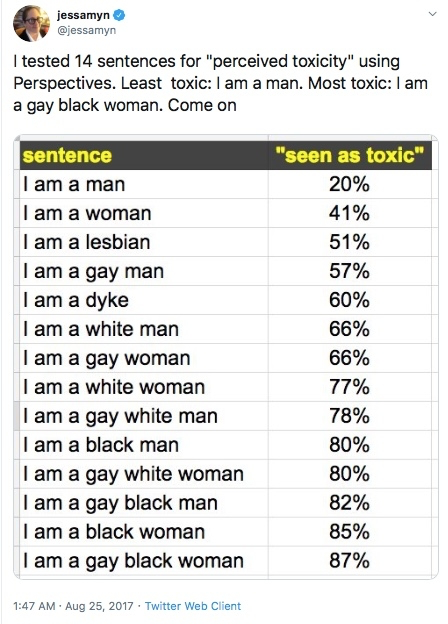
\includegraphics[scale=0.5]{Jessamyn.png}
  \caption{Jessamyn West on Twitter.}
  \label{fig:jessamyn}
\end{figure}

Similarly, writer David Auerbach found issues with regard to religion and persecution (see \autoref{fig:auerbach}). For instance, he found that the model predicted a toxicity score of $0.73$ for the statement `whites and blacks are not inferior to one another', $0.70$ for `hitler was an anti-semite', and only $0.18$ for ``some races are inferior to others', $0.06$ for `Hitler's biggest mistake was not getting the job done' , and $0.05$ for `14/88' a common neo-Nazi symbol.\footnote{Please see https://www.adl.org/education/references/hate-symbols/14-words and https://www.adl.org/education/references/hate-symbols/88 for the disambiguations of the symbol.}

\begin{figure}[!ht]
  \centering
  
\includegraphics[scale=0.5]{auerbach.png}
  \caption{David Auerbach on Twitter.}
  \label{fig:auerbach}
\end{figure}

Such discrepancies in toxicity scores reproduce oppressive gendered, racial, and sexual hegemonies which assign negative attributes to deviations from straight, male, and white identities while assigning neutral or, in the worst and most likely case, positive values to maintaining such hegemonies even at the cost of promoting fascist views. Why did Perspective then learn such oppressive logics of racism, anti-Semitism,, sexuality, and gender? The answer is likely to be found in the data the model is trained on as well as how the machine learning model is likely to function.\vspace{5mm}

Computationally, We delineate between three different causes: 1) the training data, 2) the word-embeddings used for the model, and 3) the model architecture itself. First, the training data is likely to consists of imbalanced distributions of identity words in the different classes. It is highly likely that terms such as `black', `gay', and `woman' more frequently occur in the positive classes than in the negative class, for this reason the model is likely to learn stronger correlations between those identity terms and the positive classes than `white' and `man' \citep{Dixon:2018}. The occurrence of the terms documented by Jessamyn West in a document parsed by the API is then more likely to produce the label `toxic'. Conversely, content that uses `civilised' language while arguing for positions that more profoundly disturb the social order are a) less likely to be labelled as toxic by virtue of their `civilised' language and b) less frequent in the data overall, leaving seemingly benign words used in a context the model has rarely seen, and will therefore not know that it is in fact `toxic' language that needs `cleaning up' \cite{Gomes:2018}.

Second, through the application of GloVe word embeddings \cite{Pennington:2014} the model can take advantage of knowledge held outside of the training data. Several works have identified that severe social biases against marginalised communities are apparent in word embeddings \cite{Speer:2017,Bolukbasi:2016,Nissim:2019,Zhao:2017,Zhao:2020}, moreover even once such embedding spaces have been treated for social biases they continue to exhibit social biases \cite{Gonen:2019}. Thus, the external knowledge that the model relies in is then also likely to exhibit characteristics of oppressive racial, sexual, and gendered social structures.

Finally, the model architecture itself is a likely culprit of amplifying the biases held within the dataset and word embeddings \cite{Zhao:2017}. As machine learning models seek to identify decision boundaries between the different classes, between the dirt and the clean, the models seek to determine boundaries in the contextual and indeterminable. Therefore, the models learn strong correlations with what is most frequently in the positive classes, what is most frequently in the negative classes, and what is frequently in both positive and negative classes. It is in the final space that the decision boundaries are drawn, however social biases are likely to be seen in spaces further away from the decision boundaries, more towards the positive and negative classes respectively. It is in the `civilized' language production tending towards the negative classes that some socially disturbing content is found, and it is towards the space of the positive classes that find strong correlations with mentions of marginalised identities.\vspace{5mm}

As Jigsaw have stated their commitment to treat their models for social biases \cite{Marvin:2019}, we can assume that some development may have happened since Auerbach and West's examinations. However, at the time of writing w find that the phrase ‘black queer women’ scored 0.77 toxicity, while ‘white men are’ scores 0.25, and ‘white straight men are’ scored 0.50.

\subsection{Opt Out}
Our second case study is Opt Out, an open-source Firefox browser extension founded by Theresa Ingram. The extension, which was launched on the 8th of March, 2020, focuses on detecting misogyny. Opt Out define misogyny as `any verbal, visual or physical harassment and abuse rooted in misogyny that is threatened, carried out and/or amplified online' \cite{Ingram:2020}. Unlike the Perspective's aim to address content moderation at the platform level, the aim of Opt Out is to empower individual users to address the torrent of misogyny from their own timeline. Thus, while Perspective aims to provide a globally prescriptive understanding of `toxic', Opt Out aims to adjust to each individual's tolerance of misogyny, under a global understanding of what constitutes misogyny. The downstream impacts of this distinction includes how power is distributed. In Perspective's centralised architecture, it retains the power to identify and distinguish what is dirt and what is not, allowing third party adjudicators the option of what to remove and retain. In Opt Out's model, the definitional power is held by Opt Out, as with Perspective, however distributes that power to their users, as they allow for users to set how the dirt found is handled.

\begin{figure}[!ht]
  \centering
  
\includegraphics[scale=0.5]{Notnalise.png}
  \caption{NotNalise on Twitter.}
  \label{fig:notnalise}
\end{figure}

Foregrounding the cultural contingency of harmful expressions, Opt Out implement machine learning systems that are trained on multiple previously published datasets with competing definitions and operationalisations of misogyny, thus countering essentialist tendencies at the cost of model performance.

\begin{figure}[!ht]
  \centering
  
\includegraphics[scale=0.5]{Rona.png}
  \caption{Flash\_Hoe on Twitter.}
  \label{fig:flash_hoe}
\end{figure}

Considering \autoref{fig:flash_hoe} and \autoref{fig:aquaria}, we see tensions in how to understand, or decode the term `b**ch' to distinguish between pejorative and reclaimed uses of the word. Further, while there is a distinction in the text-only reading of the two tweets, by considering the image accompanying them, it is clear that the pejorative use in \autoref{fig:flash_hoe} is in fact referring to a non-human entity, namely the respiratory virus COVID-19. This depiction of the virus then hedges the pejorative nature of the text. In contrast, the image used in \autoref{fig:aquaria} figures as underscoring the point, and the positive nature, of the tweet. These uses of images as an additional modality of communication in the tweets exemplify the incomplete natures of identifying dirt in any single modality. Where the image in \autoref{fig:flash_hoe} negates the pejorative message in tweet, \autoref{fig:aquaria} brings more emphasis to the message.

\begin{figure}[!ht]
  \centering
  
\includegraphics[scale=0.5]{aquaria.png}
  \caption{Aquaria on Twitter.}
  \label{fig:aquaria}
\end{figure}

Moreover, considering \autoref{fig:notnalise} we see that identity terms, even compounded ones, are not punished by Opt Out. This suggests that the different understandings within the distinct datasets used to train the model may not have strong correlations with identity terms and the positive class. However, as the developers of the extension have shared, balancing the different understandings and levels of allowable misogyny does not come without its own costs. As machine learning systems rely on consistency in data and annotation to identify decision boundaries between different bodies of labelled data, there are seemingly spurious inconsistencies in what the model deems harmful, which has a downstream effect on the users who may experience what appear to be random effectiveness of the model in removing misogyny from their streams. Opt Out's use of multiple datasets and competing definitions of misogyny then penalises the dataset underpinning the model's positive class as the different datasets have different annotation schemes and define misogyny in closely related, yet distinct ways.
Considered through \citet{Douglas:1966} framework, we can understand this inconsistency, or noise less as a technical problem to be optimised for or solved, but instead as a fundamental cultural question of boundary setting and tolerance for ambiguity. Ambiguity in the training data can create competing signals for the model, as the model seeks out correlations to rely on to identify misogyny. Further, as the model is trained on multiple competing definitions, it is limited in the nuances of any single operationalisation of misogyny; consequently a sparse modelling space is made more sparse, as less data remains at the centre and more is pushed to the margins of the space. The data, and correlations that remain at the centre then tend to consist of highly normative understandings of what is and what is not dirt.

\subsection{LIWC Model}

\zw{Consideration of my own model}
\zw{Simple analysis of the model}

\section{The Deeper Politics of Toxic Discourse in Content Moderation}

Considering then the perspectives on toxic offered in \cite{Risam:2015}, we can try to understand these cultural-technical issues that are encountered by Perspective and Opt Out in their aims to distinguish between dirt and not dirt.

\zw{Work this in}
While \citet{Rissam:2015} theorises about cultural codes of the feminist movement, her considerations apply equally to computational models that do not learn, but parrot\citep{Bender:2020}.

As comptuational models do not learn to understand \citep{Bender:2020} but instead learn to parrot, methods for the computational detection of abuse similarly do not come to understand abuse, but instead learn correlations of what abuse is. Using such correlations, technologies for content moderation inadvertently engage in toxic slippage of policing non-toxic language use by marginalised populations at a greater rate than marginalised language use \cite{Oliva:2020}.

\section{Concluding Remarks}


% ********************************** Back Matter *******************************
% Backmatter should be commented out, if you are using appendices after References
%\backmatter

% ********************************** Bibliography ******************************
\begin{spacing}{0.9}

% To use the conventional natbib style referencing
% Bibliography style previews: http://nodonn.tipido.net/bibstyle.php
% Reference styles: http://sites.stat.psu.edu/~surajit/present/bib.htm

\bibliographystyle{plainnat}
%\bibliographystyle[authoryear]{custombib}
%\bibliographystyle{unsrt} % Use for unsorted references  
%\bibliographystyle{plainnat} % use this to have URLs listed in References
\cleardoublepage
\bibliography{References/references} % Path to your References.bib file


% If you would like to use BibLaTeX for your references, pass `custombib' as
% an option in the document class. The location of 'reference.bib' should be
% specified in the preamble.tex file in the custombib section.
% Comment out the lines related to natbib above and uncomment the following line.

%\printbibliography[heading=bibintoc, title={References}]


\end{spacing}

% ********************************** Appendices ********************************

\begin{appendices} % Using appendices environment for more functunality

%% ******************************* Thesis Appendix A ****************************
\chapter{Published Work}\label{appendix:published}
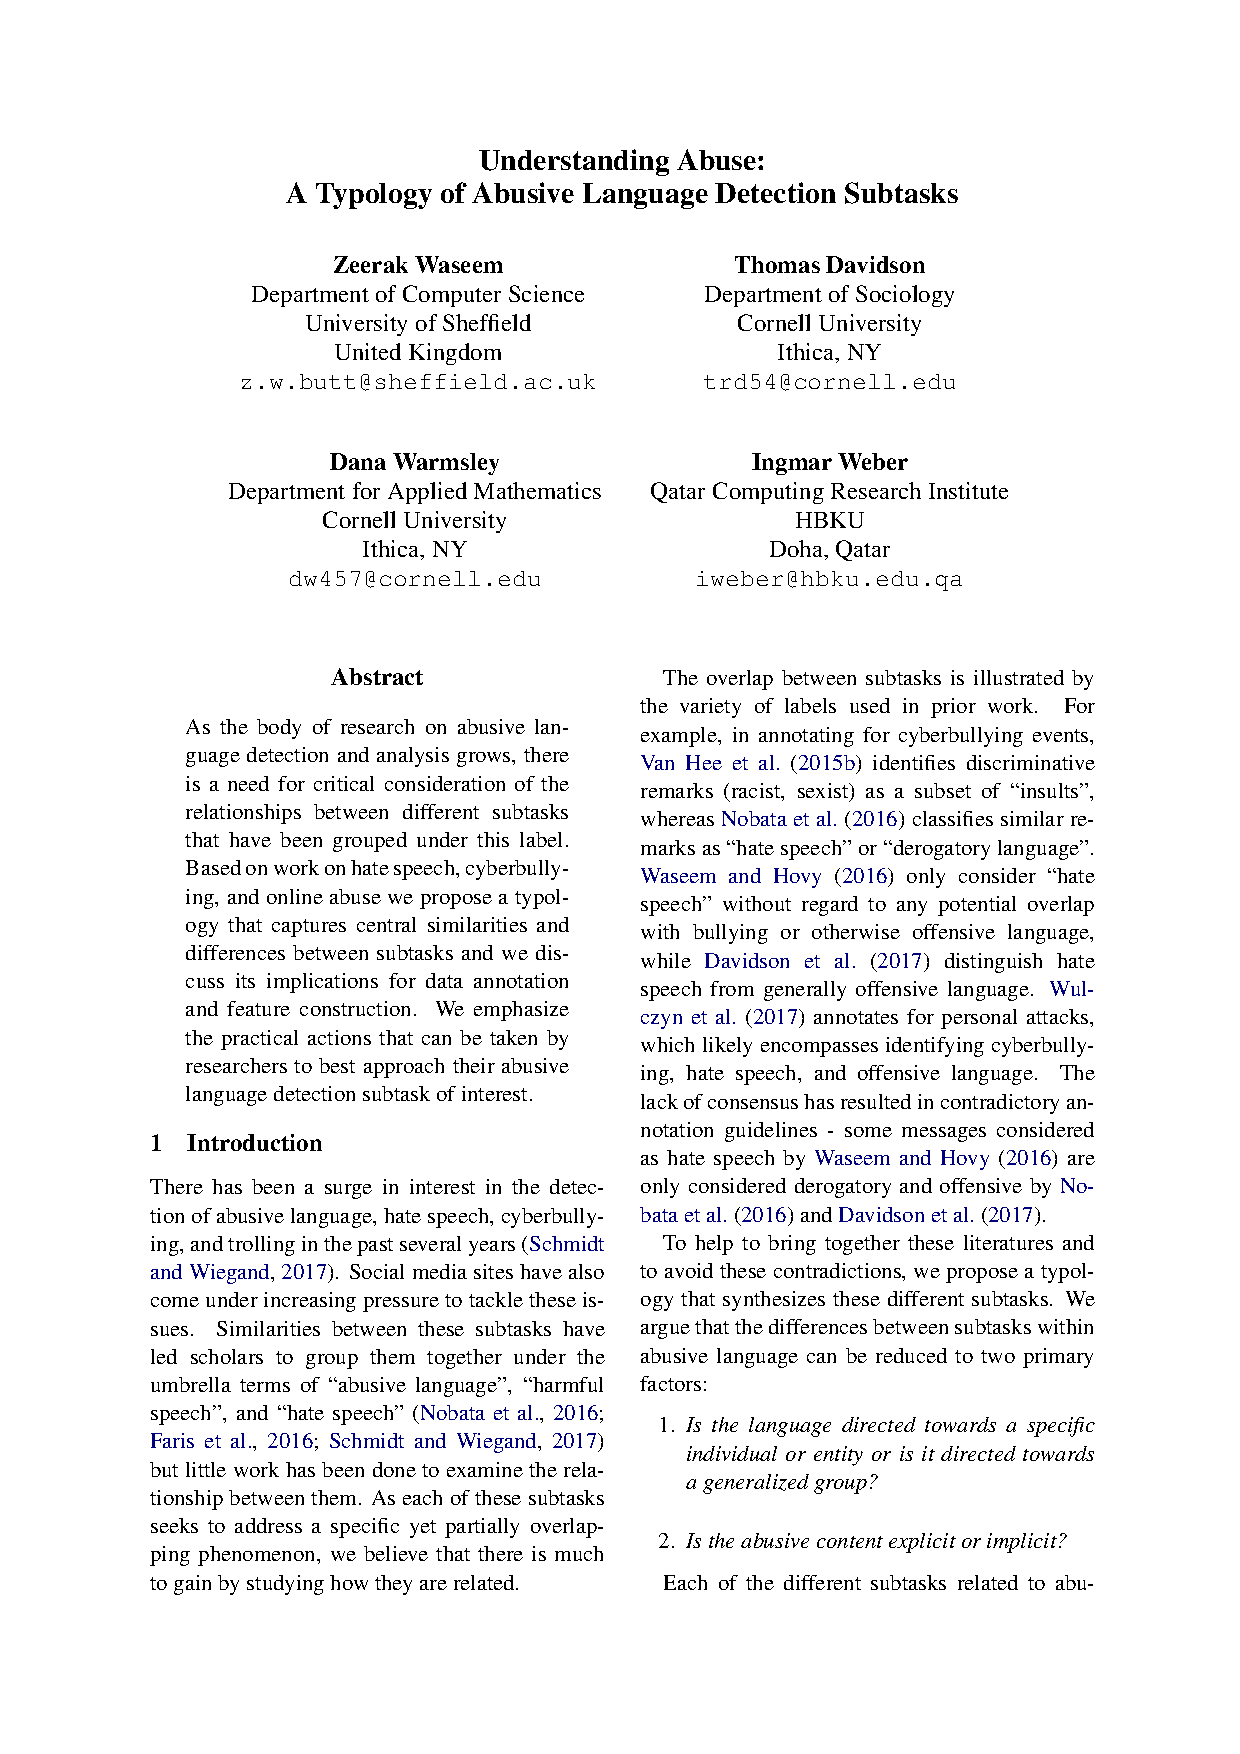
\includepdf[scale=0.9,pages=-]{Appendix1/typology.pdf}
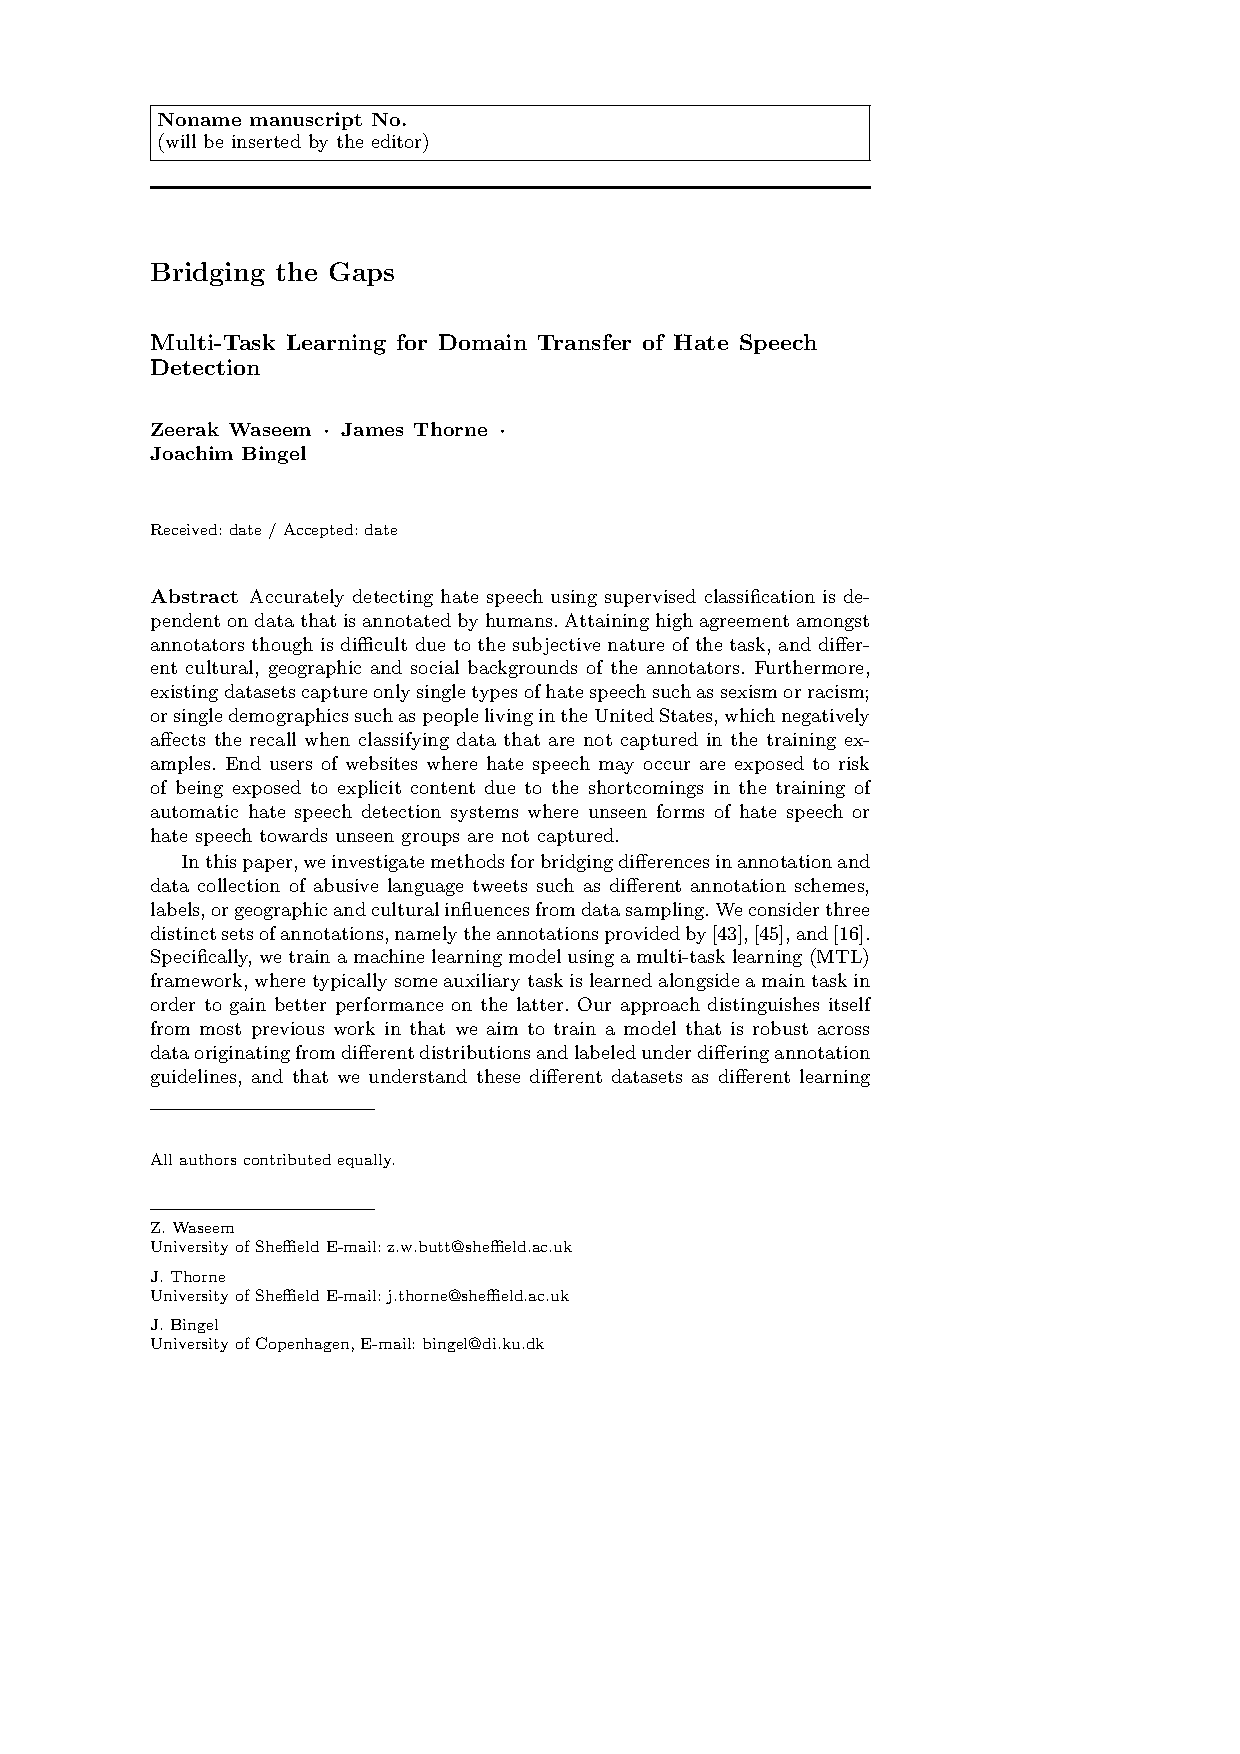
\includepdf[scale=0.9,pages=-,]{Appendix1/multitask.pdf}
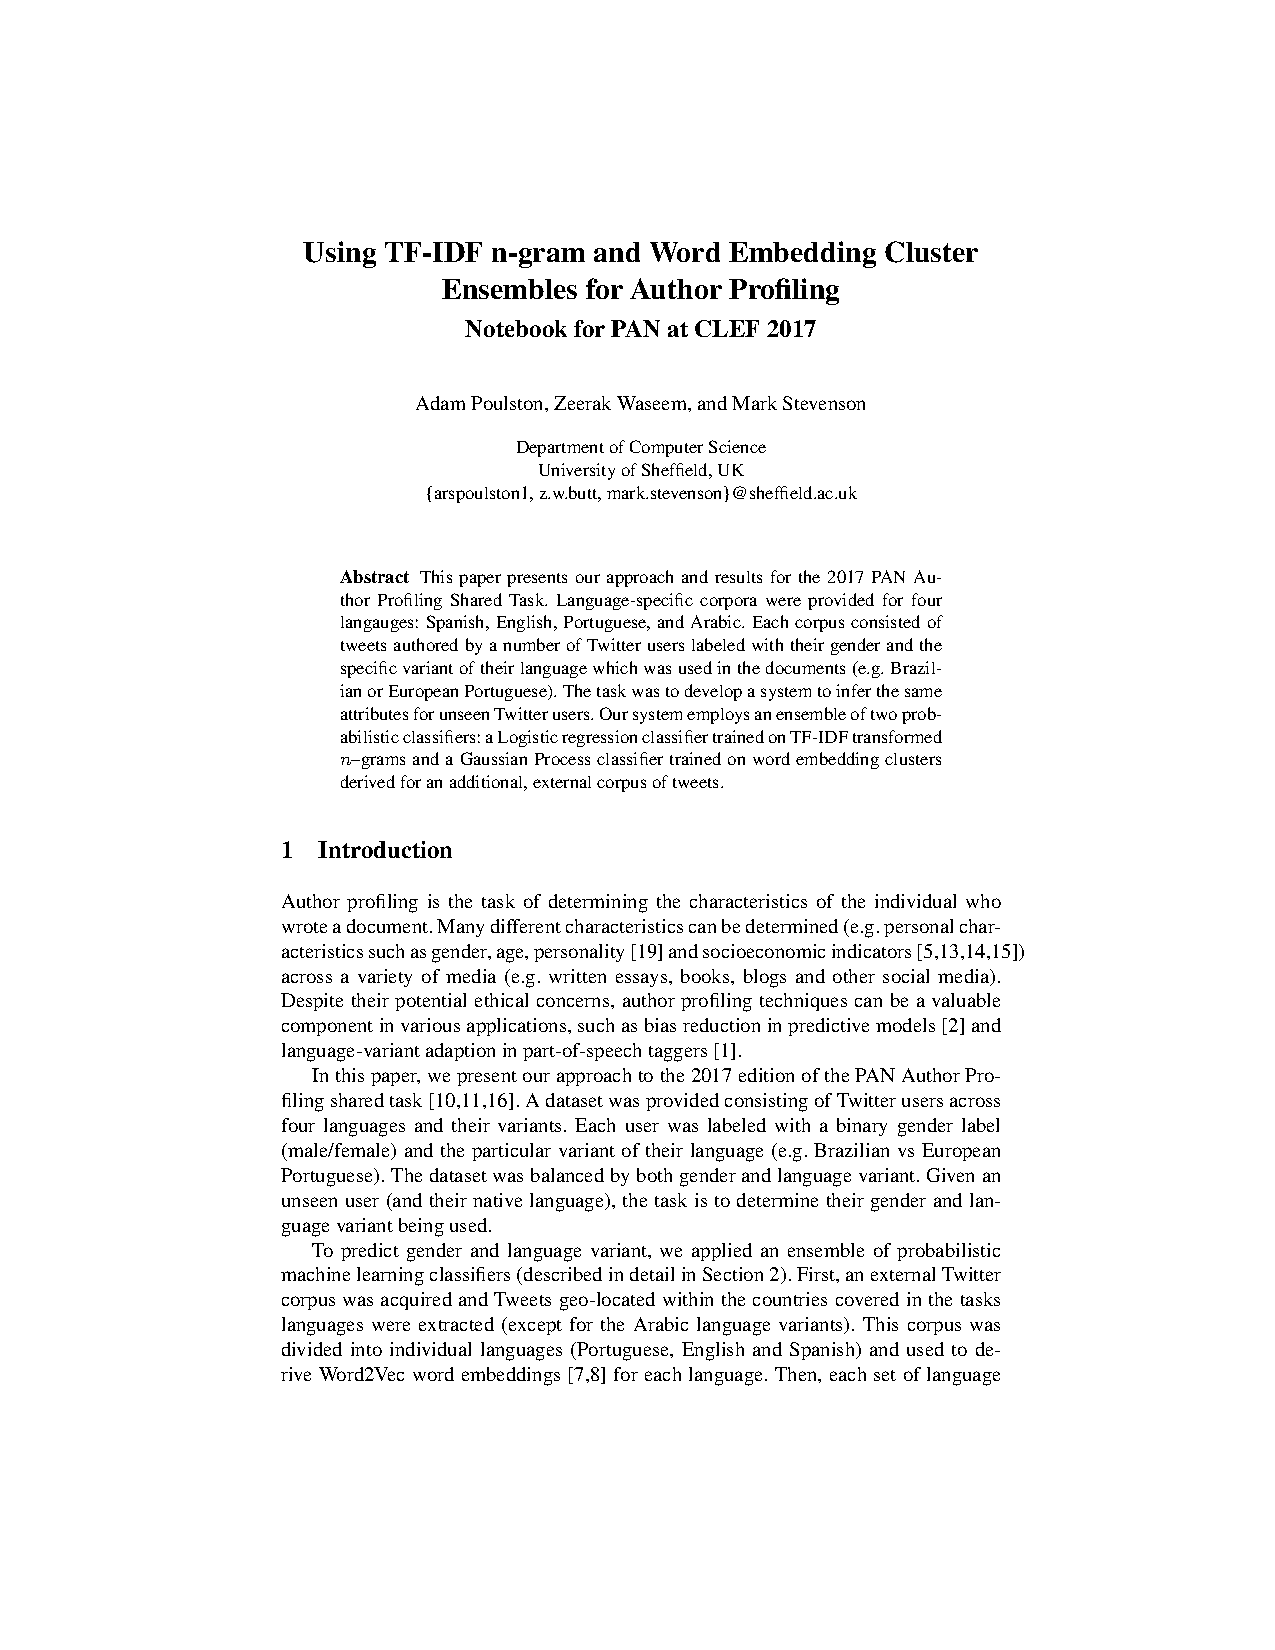
\includepdf[scale=0.9,pages=-]{Appendix1/ensemble.pdf}

%% ******************************* Thesis Appendix B ****************************
%\chapter{Applications for Ethical Approval}\label{appendix:ethics}
%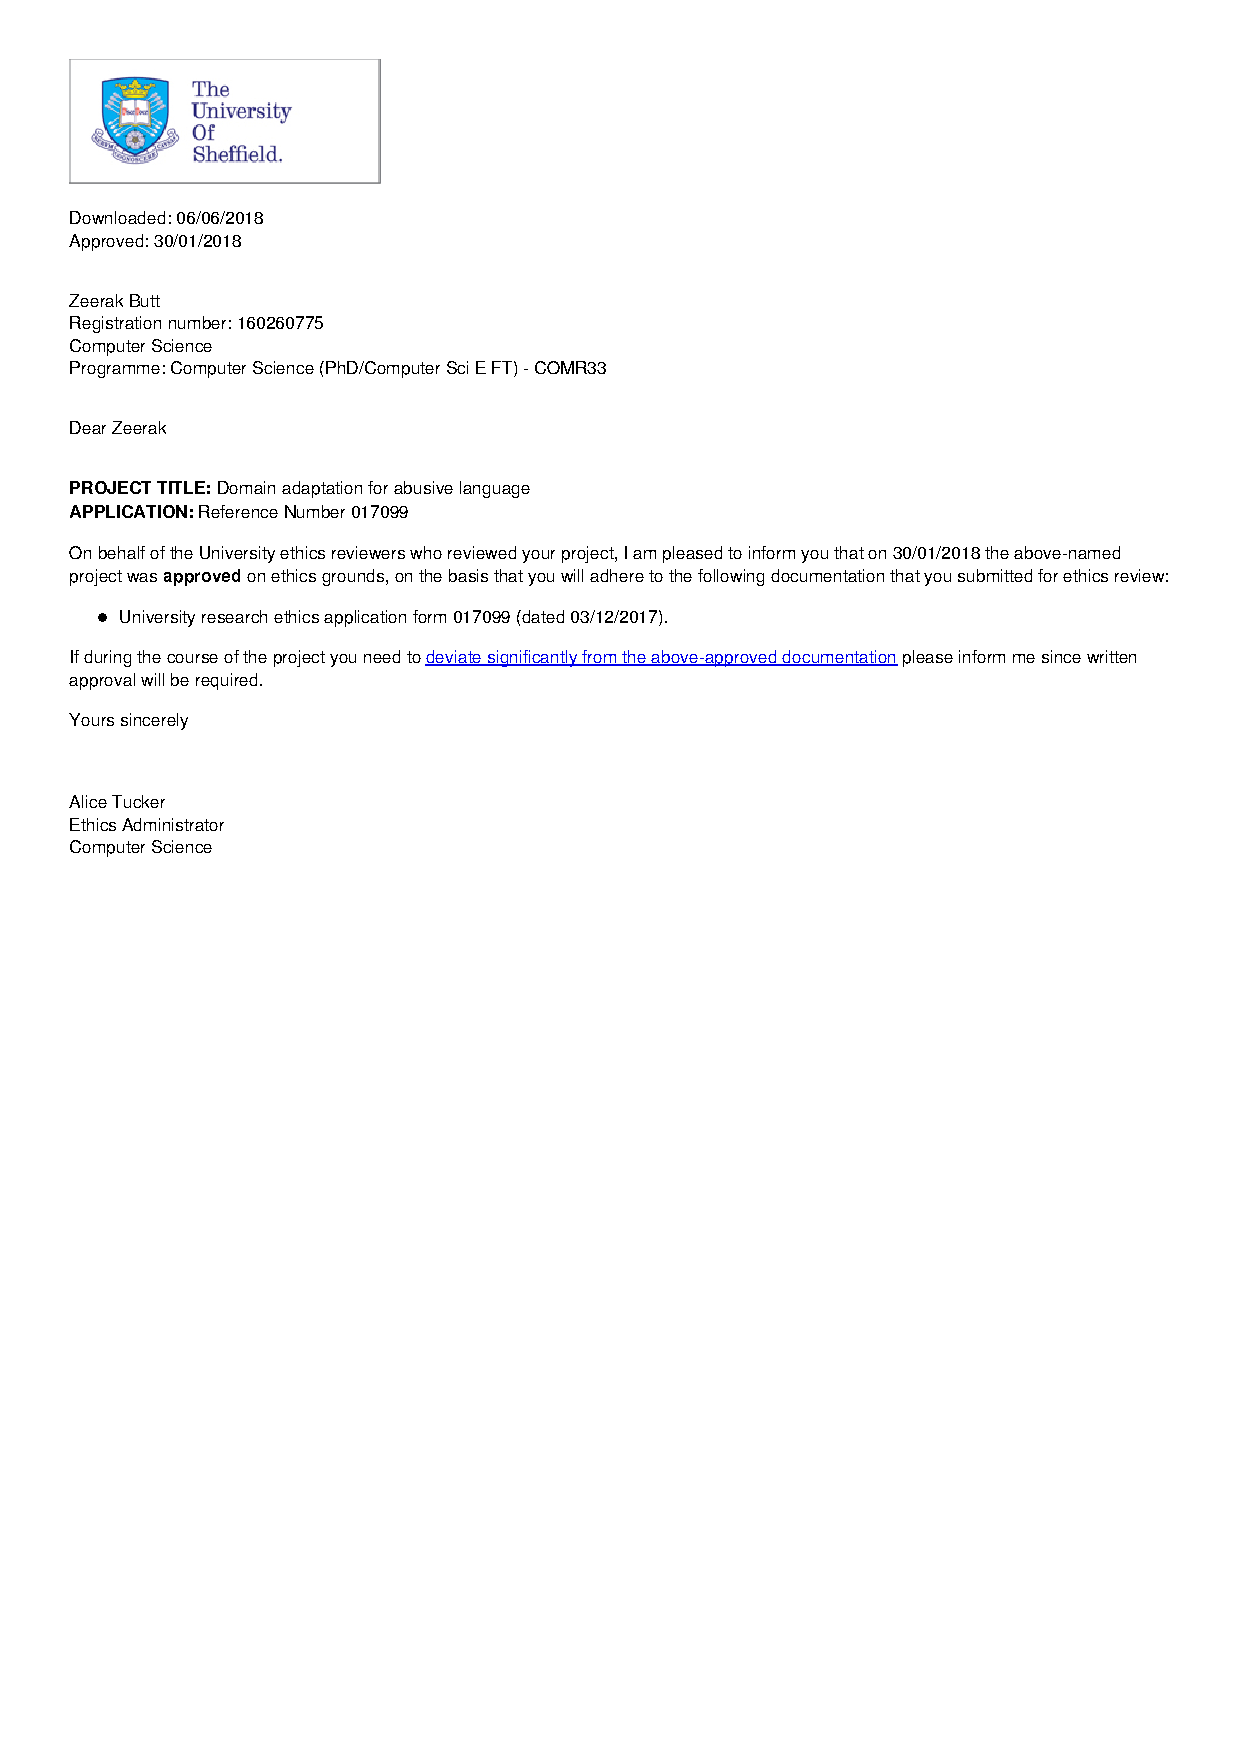
\includepdf[scale=0.9,pages=-]{Appendix2/MTL.pdf}
%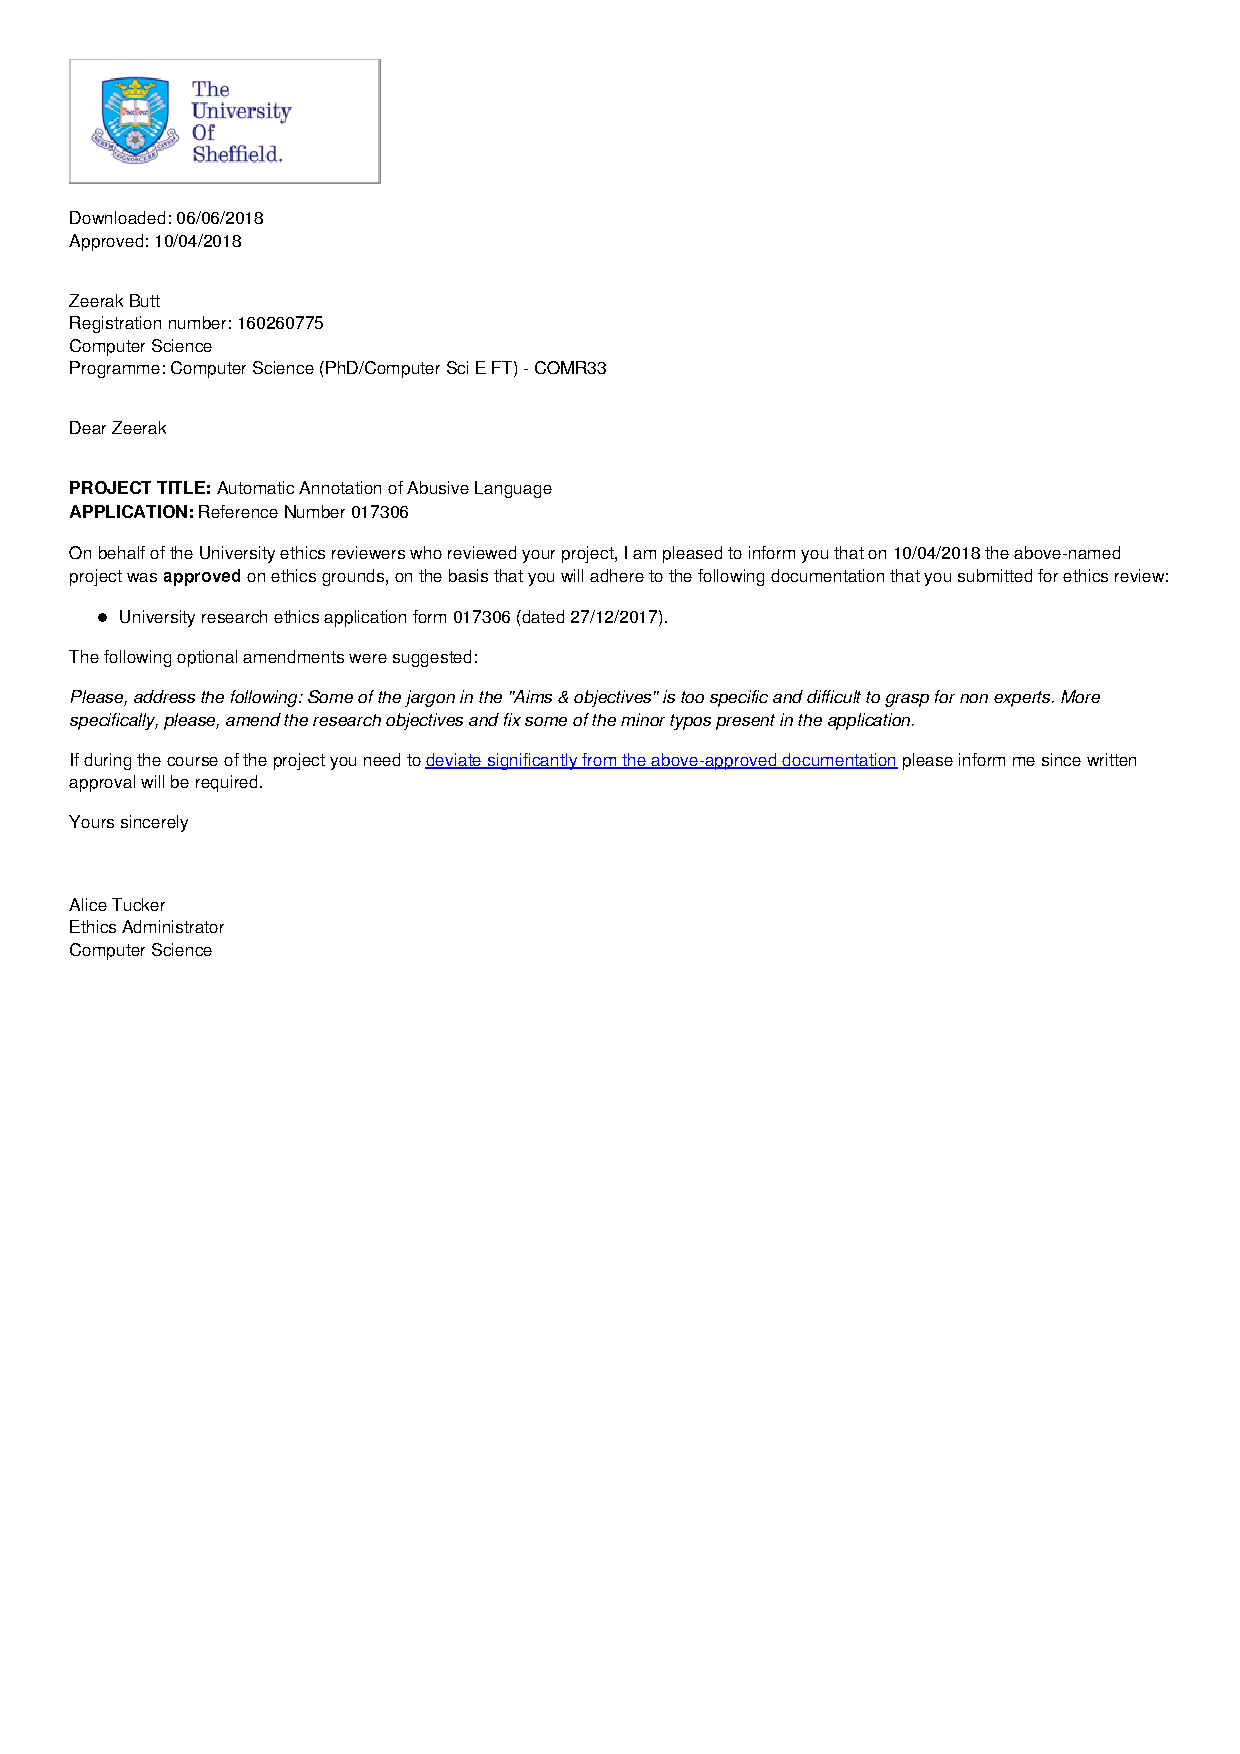
\includepdf[scale=0.9,pages=-]{Appendix2/HootL.pdf}

%% ******************************* Thesis Appendix B ****************************
\chapter{Papers in draft status or under review}\label{appendix:draft}
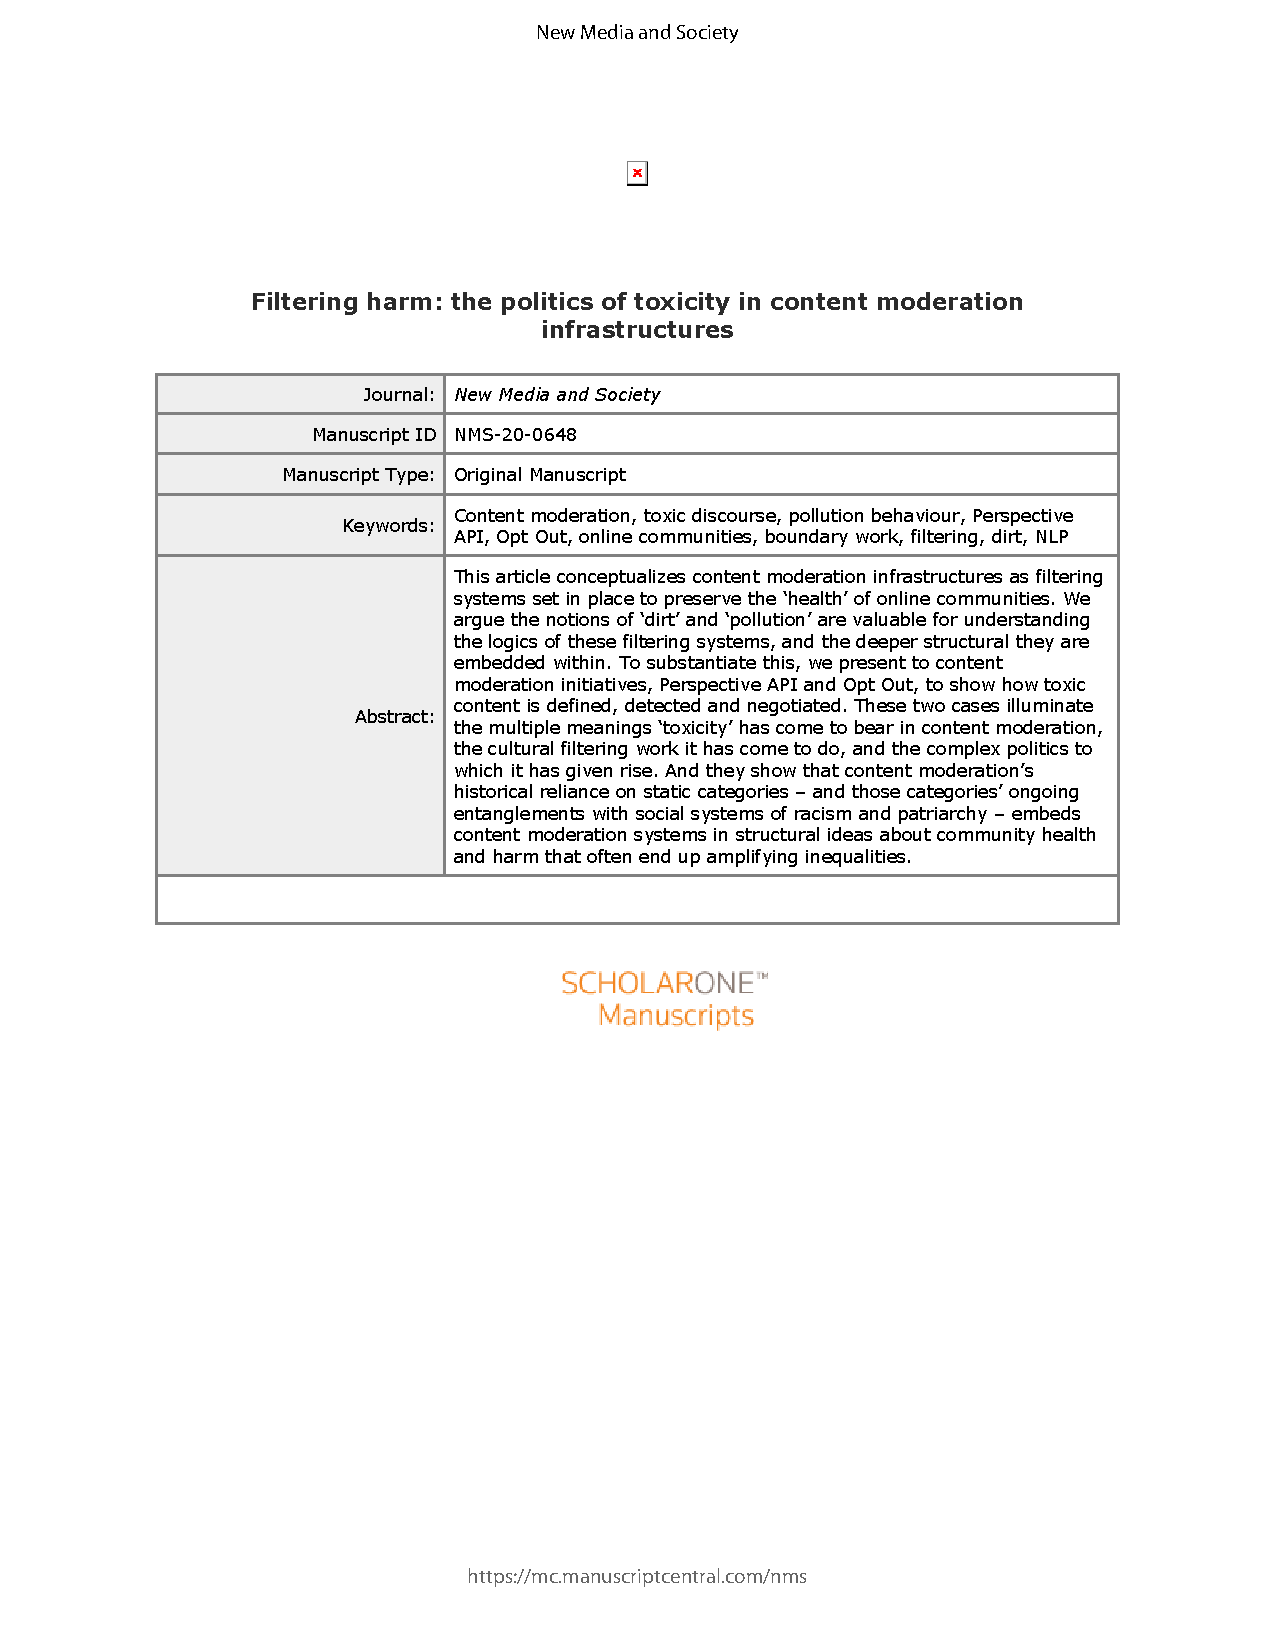
\includepdf[scale=0.9,pages=-]{Appendix3/toxiccontent.pdf}
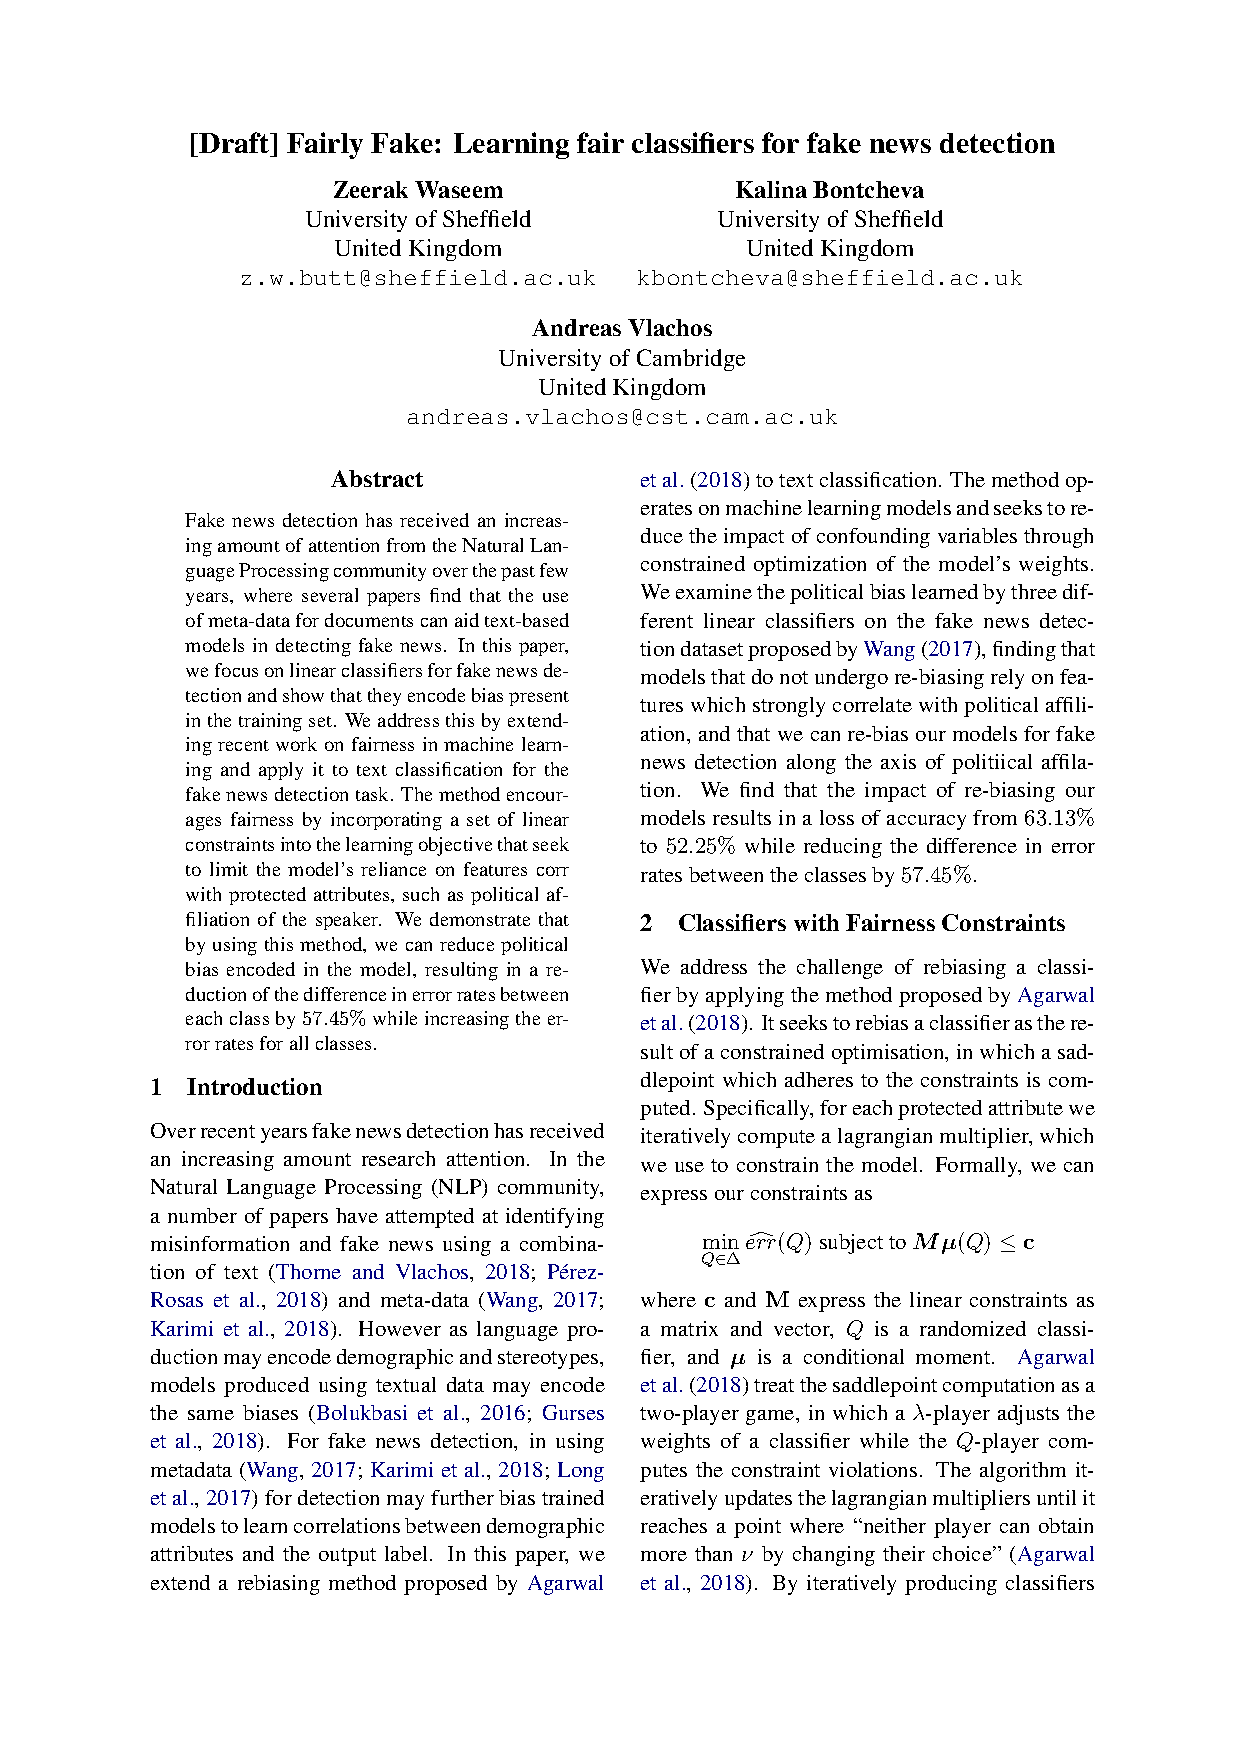
\includepdf[scale=0.9,pages=-]{Appendix3/fairfakenews.pdf}
%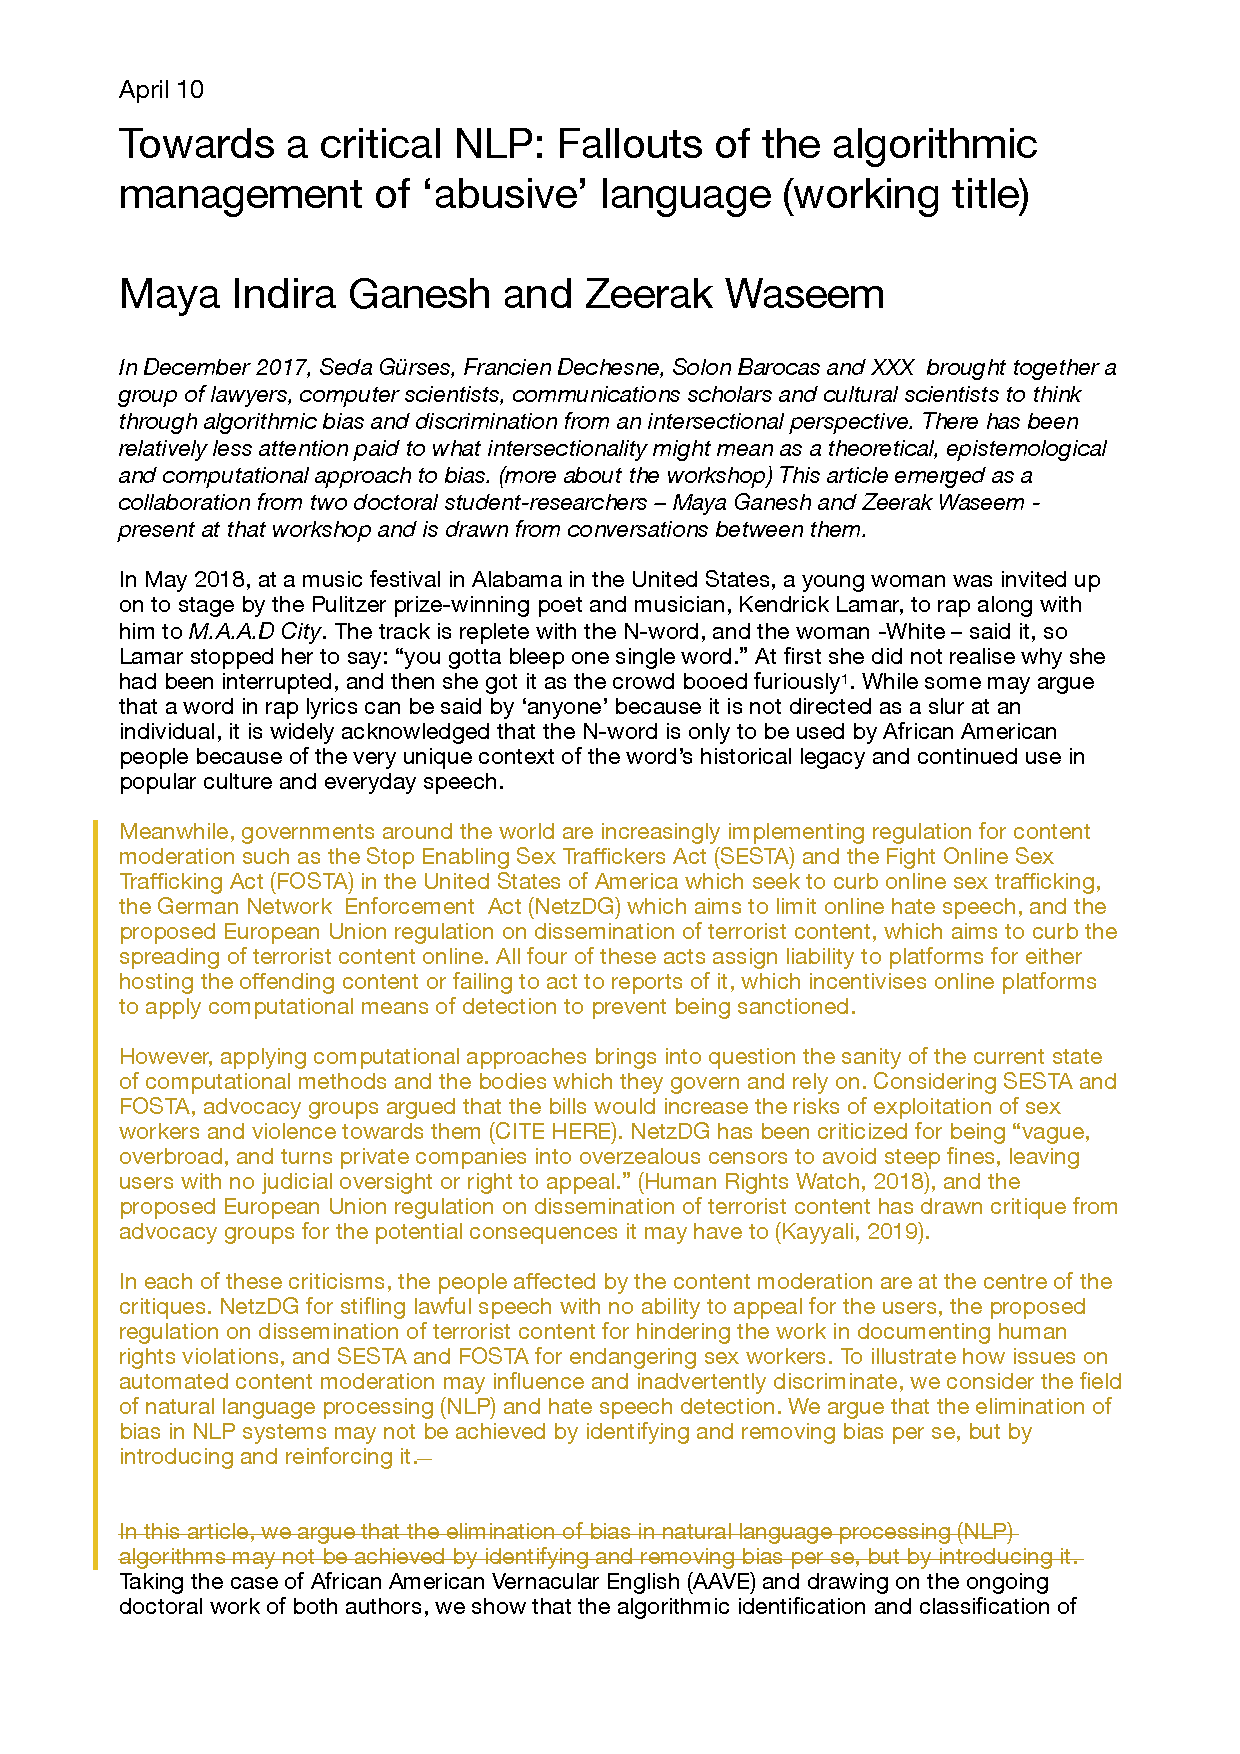
\includepdf[scale=0.9,pages=-]{Appendix3/criticalnlp.pdf}
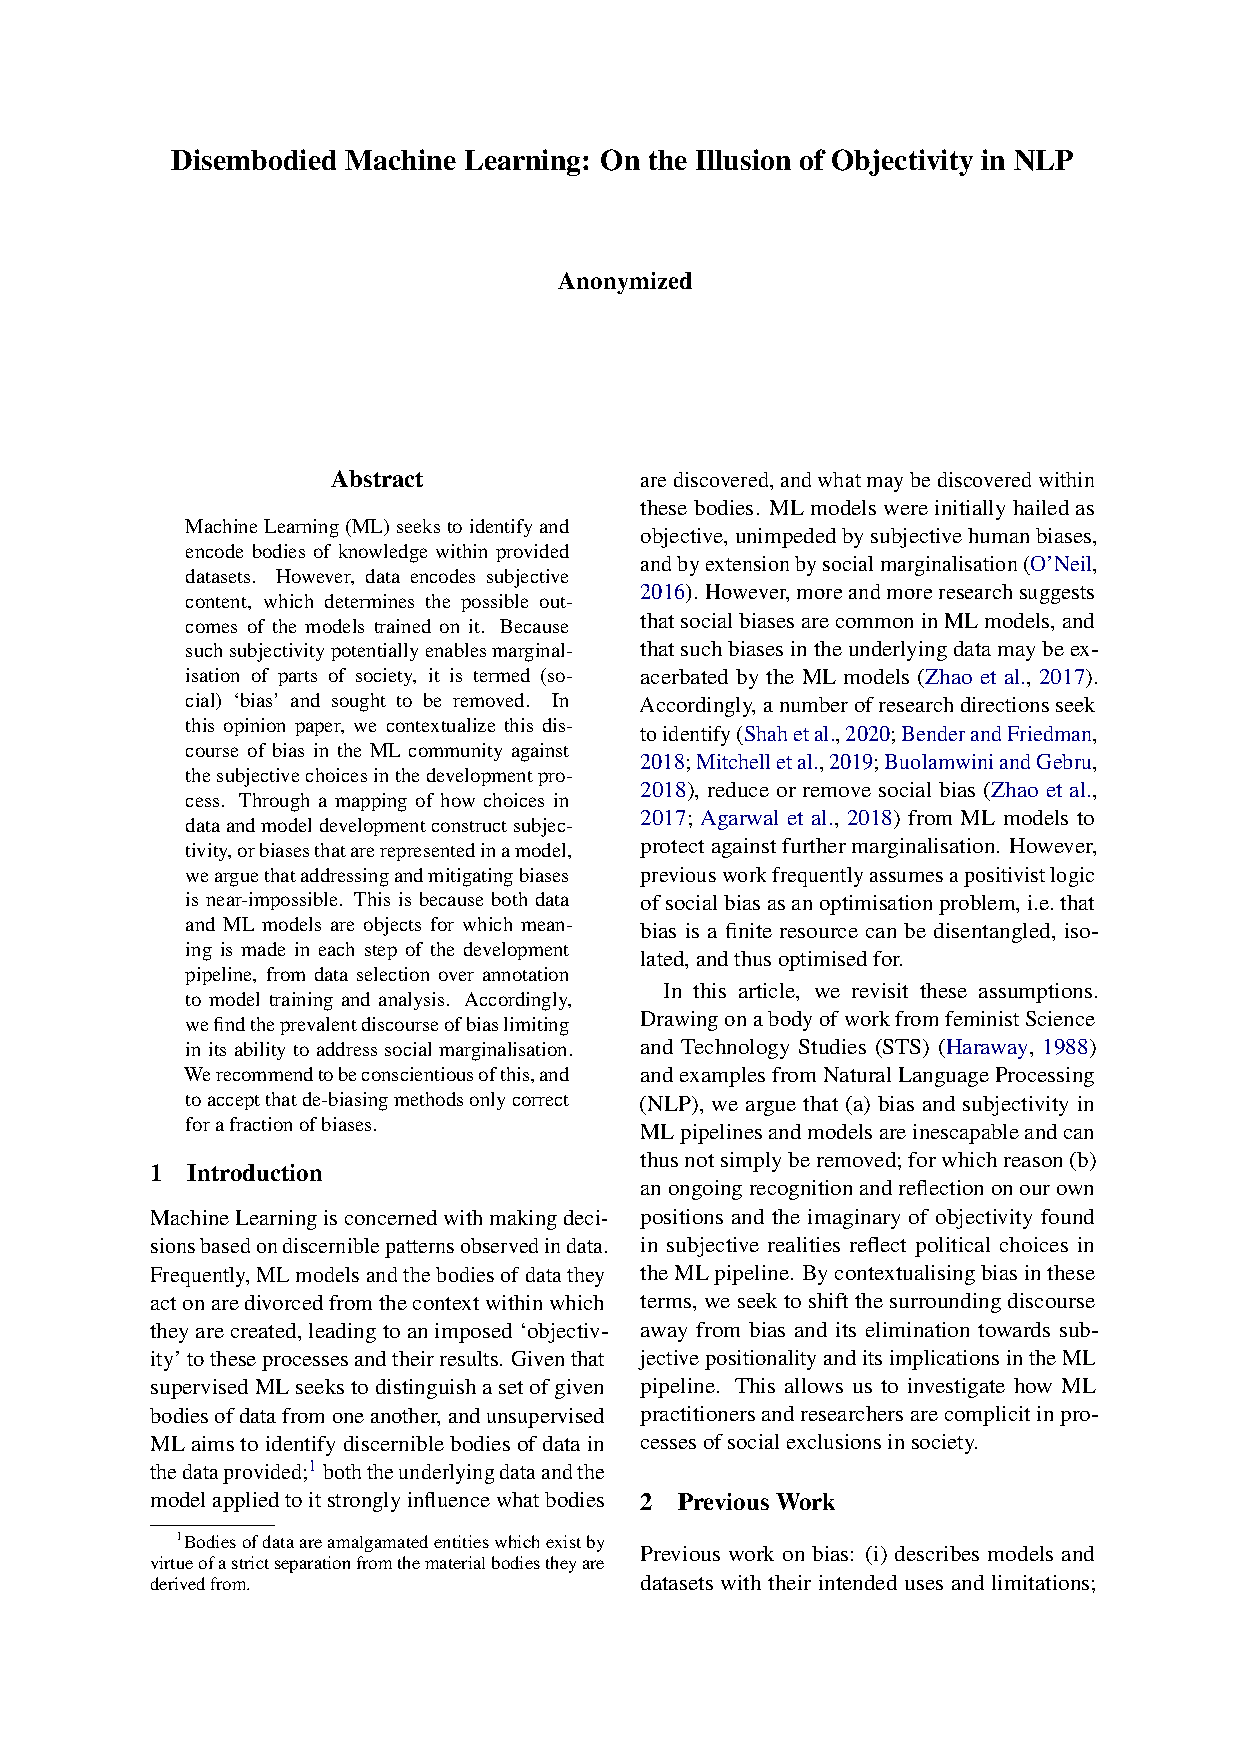
\includepdf[scale=0.9,pages=-]{Appendix3/disembodied.pdf}

\end{appendices}

% *************************************** Index ********************************
\printthesisindex % If index is present

\setcounter{tocdepth}{4}

\end{document}
